\documentclass[a4paper,twoside,openright,12pt]{memoir}

%MAXIMUM - 250 PAGES (about 50k words)
%AIM - 100-150 PAGES (40k WORDS) PLUS APPENDICES

% Memoir linespacing
\DoubleSpacing

% LaTeX packages
\usepackage{amsmath}
\usepackage{amsfonts}
\usepackage{amssymb}
%\usepackage{mathabx}
\usepackage{bigfoot}
\usepackage{bm}
\usepackage{caption}
\usepackage{color}
\usepackage{graphicx}
\usepackage{indentfirst}
\usepackage{subcaption}
\usepackage{inconsolata}
\usepackage{siunitx}
% \usepackage{chemformula}
\usepackage{microtype}

\usepackage[dvipsnames]{xcolor}
%\usepackage{deluxetable}

% remove paragraph indent
%\setlength{\parindent}{0in}


% %\usepackage[pdfauthor={Mark Hammond},pdftitle={Thesis},colorlinks=true]{hyperref}%
% %
% \hypersetup{
%   colorlinks=true,
%   citecolor=MidnightBlue,
%   urlcolor=MidnightBlue,
%   linkcolor=Black
%   %linkcolor=BrickRed
% }

%\usepackage[utf8]{inputenc}
% \usepackage[
%   safeinputenc,
%   style=phys,
%   backend=biber,
%   sorting=none,
%   minnames=10,
%   maxnames=10,
%   biblabel=brackets
% ]{biblatex}
% \addbibresource{references.bib}

%\usepackage[no-math]   {fontspec}
%\setmainfont{Minion Pro}

\usepackage{MinionPro}
%\defaultfontfeatures{Mapping=tex}
%\setmainfont{Minion Pro}
%\usepackage[italic]{mathastext}


% \usepackage{libertine}
%\usepackage{txfonts}


%\usepackage[MnSymbol]{mathspec}

%\setmainfont{Minion Pro}
%\setmathfont[range=\mathup/{num,latin,Latin,greek,Greek}]{Minion Pro}
%\setmathfont[range=\mathbfup/{num,latin,Latin,greek,Greek}]{MinionPro-Bold}
%\setmathfont[range=\mathit/{num,latin,Latin,greek,Greek}]{MinionPro-It}
%\setmathfont[range=\mathbfit/{num,latin,Latin,greek,Greek}]{MinionPro-BoldIt}

\usepackage{lipsum}
\usepackage{oxfordthesis}
\usepackage{xr}
\usepackage{xr-hyper}

\usepackage[round]{natbib}

% Title / Author / Date / Degree / etc.
\thetitle{The Atmospheric Circulation of Tidally Locked Terrestrial Exoplanets}
\theauthor{Mark Hammond}
\degreedate{Trinity Term 2019}
\degree{Doctor of Philosophy}
\college{Hertford College}
\university{University of Oxford}


\usepackage[
	pdftitle={\oxfthetitle},
	pdfauthor={\oxftheauthor},
	pdfsubject={Thesis for the Degree of \oxfdegree, \oxfdegreedate},
	pdfborder=0,
	bookmarks=true,
	bookmarksnumbered=true,
	bookmarksopen=true,
	bookmarksopenlevel=1,
	plainpages=false,
	pdfpagelabels=true,
	colorlinks=true,
    citecolor=MidnightBlue,
	  urlcolor=MidnightBlue,
		linkcolor=Black
]{hyperref}
\usepackage{memhfixc}

% Your Macros File Here
% Useful macros
\newcommand{\figref}[1]{Figure~\ref{fig:#1}}
\newcommand{\figsref}[2]{Figures~\ref{fig:#1} and~\ref{fig:#2}}
\newcommand{\figsdash}[2]{Figures~\ref{fig:#1} -- \ref{fig:#2}}
\newcommand{\Figref}[1]{Figure~\ref{fig:#1}}
\newcommand{\Figsref}[2]{Figures~\ref{fig:#1} and~\ref{fig:#2}}
\newcommand{\Figsdash}[2]{Figures~\ref{fig:#1} -- \ref{fig:#2}}
\newcommand{\Secref}[1]{Section~\ref{#1}}

%\renewcommand\secheadstyle{\setSpacing{0.95}\Large\bfseries\memRTLraggedright}

\setsecheadstyle{\large\bfseries}
\setsubsecheadstyle{\normalsize \bfseries}
\setsubsubsecheadstyle{\normalsize \bfseries}

\setlrmarginsandblock{3.5cm}{3.5cm}{*}
\setulmarginsandblock{3.5cm}{*}{1}
\checkandfixthelayout


\setcounter{tocdepth}{1}
\settocdepth{section}
% Main document

\begin{document}
\begin{SingleSpace}
\titlepage
\end{SingleSpace}

\frontmatter

% \pagestyle{plain}


%\begin{dedication}
Dedicated to whomever
\end{dedication}


\begin{abstract}
  This thesis aims to understand the global circulation of tidally locked lava planets, and how to interpret observations of them.
\end{abstract}


\cleardoublepage

\begin{acknowledgements}
  \lipsum[1]
\end{acknowledgements}



\cleardoublepage

\tableofcontents
% \listoffigures

\mainmatter


% equation spacing
\setlength{\abovedisplayskip}{-5pt}
\setlength{\belowdisplayskip}{15pt}

\setlength{\abovedisplayshortskip}{-5pt}
\setlength{\belowdisplayshortskip}{15pt}

%checkcites --unused main.aux chapters/conclusion.aux chapters/soc-lava-planets.aux chapters/new-linking-climate-55cnce.aux chapters/new-wave-mean-flow.aux chapters/new-eqm-zonal-flow.aux chapters/lava-planets.aux chapters/introduction.aux appendices.aux

% Overall

% draft -- marked up --  edited -- final markup -- final edit done -- spellchecked -- final check


% Abstract and Intro -- final edit done
% Review -- final edit done
% C3 -- final edit done
% C4 -- final edit done
% C5 -- final edit done
% C6 -- final edit done
% Conclusions -- final edit done
% Appendices -- final edit done

%%%%%%%%%%%%%%%
%TODO



%% Next week
% Print at work on Monday
% Bind on Monday
% Submit on Tues






%%%%%%%%%%%%%%%





%%%%%%%%%%%%%%%
%%% DONE

% 24/09
% Replot all GCM and check
% Edit C3 to say that jet level fluxes differ in mean vert term
% Markup abstract
% Edit C5 with both markup
% Fix URLs

% 25/09
% Edit C6 from 6.3
% Edit C7
% Edit appdx
% Edit C1
% Edit C2
% Edit abstract

% 26/09
% Edit C4
% Edit C3
% Dad C4 edits


%The atmospheric circulation of tidally locked terrestrial exoplanets.(, with applications to lava planets)


\chapter{Introduction}\label{sec:intro}
%\addcontentsline{toc}{chapter}{\nameref{sec:intro}}
% \vspace{0.5cm}
% \chapterprecishere{``Any finite number divided by infinity is as near to nothing as makes no odds, so the average population of all the planets in the Universe can be said to be zero. From this it follows that the population of the whole Universe is also zero, and that any people you may meet from time to time are merely the products of a deranged imagination.''\par\raggedleft--- \textup{Douglas Adams}, The Restaurant at the End of the Universe}

% \vspace{0.5cm}

Exoplanets orbit stars other than the Sun. Over the past two decades since the first was discovered, new types of exoplanet have been discovered unlike anything in the Solar System. Tidally locked planets, where the same side of the planet always faces its star, are among the most striking examples. The global circulation of an atmosphere that is only heated on one side is very different to anything seen in the Solar System. This thesis considers the formation and behaviour of this global circulation, and investigates a case study of an observed tidally locked terrestrial planet.

Tidally locked planets appear to be common despite their unusual behaviour. Figure \ref{fig:tide-locked-population} shows the exoplanets listed on the NASA Exoplanet Archive\footnote{\url{exoplanetarchive.ipac.caltech.edu}} at the time of writing plotted by stellar masses and semi-major axes. All the planets below the line were estimated to be tidally locked by the simple estimate in \citet{pierrehumbert2018review}. These planets are also generally more easily characterised due to their proximity to their host stars \citep{crossfield2015observations}. This may have created a detection bias, where we are more likely to find tidally locked planets. However, it means that they make up many of the best observational targets, so a theoretical understanding of them will be vital to making the most of upcoming measurements.

% \clearpage
\begin{figure}
  \centering
    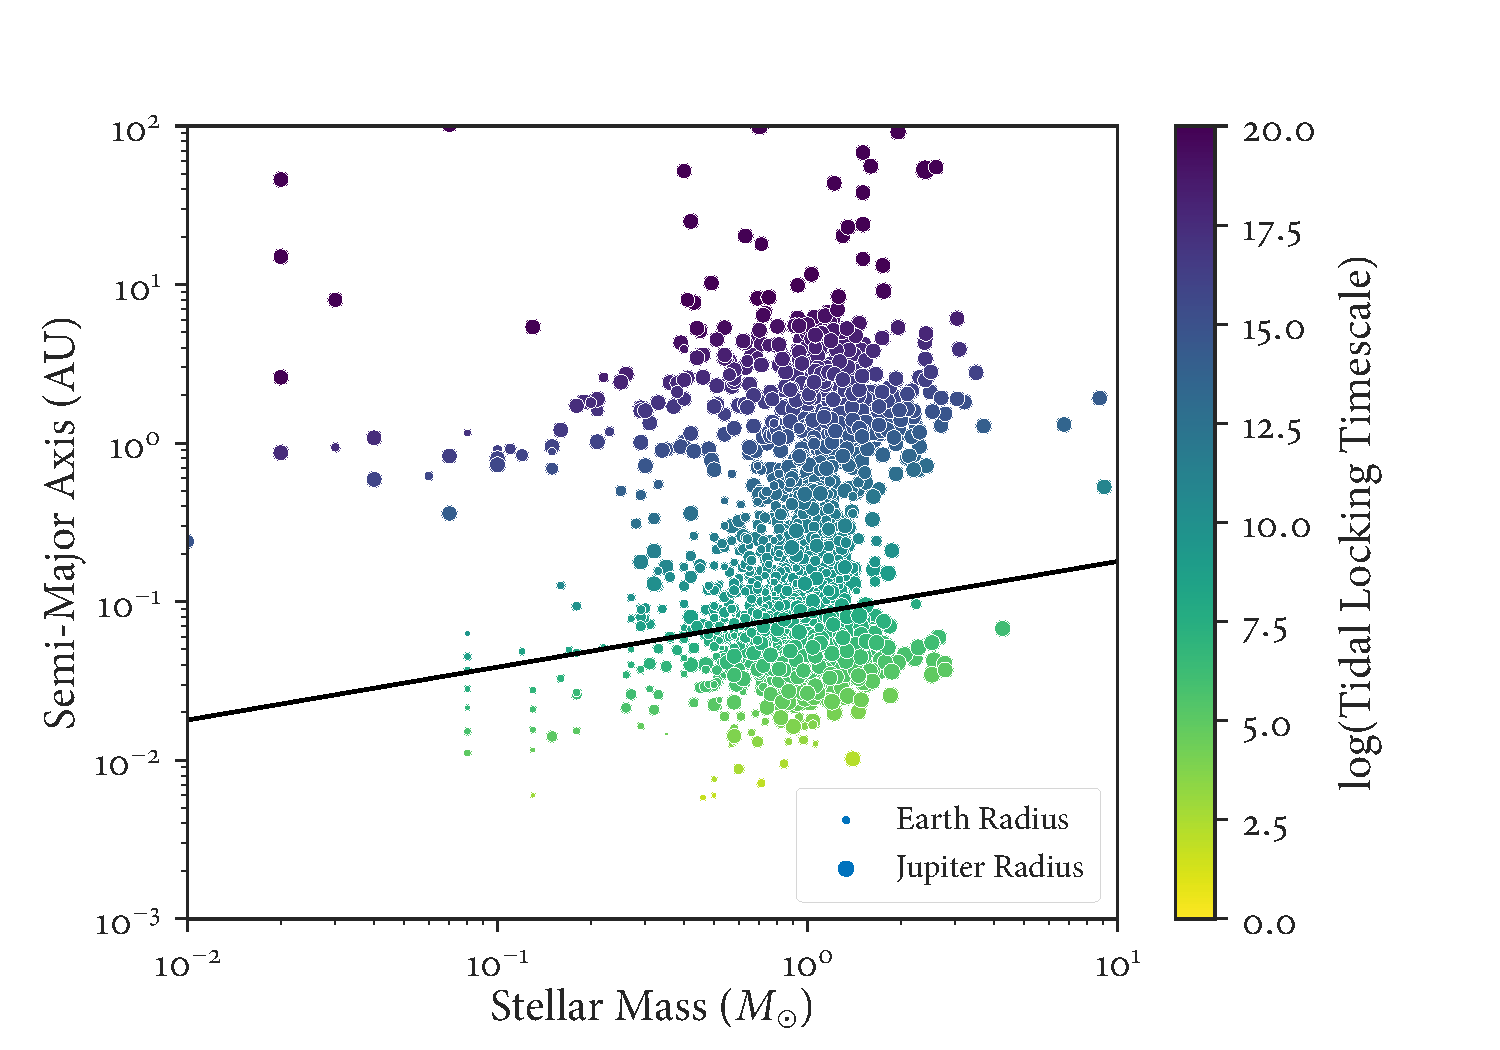
\includegraphics[width=1.0\textwidth]{figures/introduction/tide-locked-population.pdf}
    \caption{The population of known exoplanets plotted by semi-major axis and stellar mass. All the planets below the line have a timescale to reach a tidally locked state of less than 0.1 billion years, so are expected to be in this state. Chapter \ref{ch:lava-planets} explains how this timescale is calculated.}\label{fig:tide-locked-population}
\end{figure}
% \clearpage

% This thesis investigates the atmospheric circulation of tidally locked terrestrial planets.

 Current observations and simulations show that these planets have unique atmospheric dynamics, but the mechanisms for the formation of their global circulation and its effects on planetary climate are not fully understood \citep{heng2015review, pierrehumbert2018review}. The circulation governs the temperature structure of the atmosphere, affecting atmospheric stability, observations of composition, and many other important features.

This thesis has two main themes. In the first part, Chapters \ref{ch:eqm-zonal-flow} and \ref{ch:wave-mean-flow} address the theoretical circulation of terrestrial tidally locked planets and its observational consequences. In the second part, Chapters \ref{ch:linking-climate-55cnce} and \ref{ch:clouds-lava-planets} apply this theory to a case study of the ``lava planet'' 55 Cancri e, using a variety of models to interpret observations of its thermal emission.

The two themes of the thesis are reviewed in Chapter \ref{ch:lava-planets}, ``The Atmospheric Circulation of Tidally Locked Exoplanets'', which discusses relevant work on the subject of tidally locked exoplanets, focusing on the tidal locking process and the resulting atmospheric circulation. It introduces the planet 55 Cancri e, and discusses its observational characterisation to date.

In Chapter \ref{ch:eqm-zonal-flow}, ``The Gierasch-Rossow-Williams Mechanism on Tidally Locked Planets'', I propose a mechanism for the formation of the zonal flow on tidally locked planets. It shows that the meridional circulation is vital to this flow, and uses the equilibrium angular momentum fluxes predicted by the mechanism to explain the behaviour of a suite of atmospheric simulations.

Chapter \ref{ch:wave-mean-flow}, ``Wave-Mean Flow Interactions in Tidally Locked Atmospheres'', is based on \citet{hammond2018wavemean}. I linearise the shallow-water model of \citet{showman2011superrotation} about the equatorial jet discussed in Chapter \ref{ch:eqm-zonal-flow}, and show how the response to stationary forcing explains the form of the global circulation in GCM simulations. This shows that the ``hot-spot shift'' is a result of the interaction of forced stationary waves with the zonal flow, rather than simple advection of heat by the zonal flow.

Chapter \ref{ch:linking-climate-55cnce}, ``Linking the Climate and Thermal Phase Curve of 55 Cancri e'', is adapted from \citet{hammond2017climate}. It compares simulations of the atmosphere of the tidally locked planet 55 Cancri e to the observations of \citet{demory201655cnce}, to constrain the properties of the atmosphere. The observed day-night contrast can be matched with one set of parameters, and the observed hot-spot shift can be matched with another simulation. It is only possible to match the observations completely by adding an estimate of the effect of night-side cloud formation.

In Chapter \ref{ch:clouds-lava-planets}, ``Phase-Resolved Emission Spectra of Potential Climates on 55 Cancri e'', I use an improved model with more realistic radiative transfer to follow up the work in Chapter \ref{ch:linking-climate-55cnce}. The new realistic simulations still obey the scaling relations in Chapter \ref{ch:linking-climate-55cnce}, and are qualitatively similar to the simulation results in the idealised grey-gas model. I show that the simulations with surface pressures of 10 bar do not have phase shifts in their thermal emission at any wavelength, but that a simulation with a surface pressure of 100 bar does have an observable hot-spot shift. I suggest that terrestrial atmospheres with a hot-spot shift will not have a peak offset in their thermal phase curve, unless their atmospheres are sufficiently thick. The chapter concludes that the hot-spot shift observed by \citet{demory201655cnce} is evidence for an atmosphere thicker than 10 bar and with a higher molecular weight than H$_{2}$.

The conclusions in Chapter \ref{ch:conclusions} summarise the results of each chapter, and discuss their significance and the possibility of further work. The first part of the thesis shows how the global circulation of tidally locked planets is governed by their meridional circulation and the stationary waves produced by day-night forcing. I will conclude that the shallow-water models of the formation of zonal flow and a hot-spot shift on a tidally locked planet match GCM simulations, and suggest how the predictions of these models could be tested by observations. The second part of the thesis shows that the observed thermal phase curve of 55 Cancri e is evidence for a thick atmosphere with a surface pressure over 10 bar, with a mean molecular weight greater than H$_{2}$. I will conclude that this thesis has produced a consistent description of the formation of the global circulation of tidally locked terrestrial planets, and suggest future directions for modelling and observations.



% \bibliographystyle{unsrtnat}
% \bibliography{../references.bib}

\begin{SingleSpace}
\chapter{The Atmospheric Circulation of Tidally Locked Exoplanets}\label{ch:lava-planets}
%\addcontentsline{toc}{chapter}{\nameref{ch:lava-planets}}

% \vspace{0.5cm}
% \chapterprecishere{``One face is forever sunlit, and one forever dark, and only the planet's slow liberation gives the twilight zone a semblance of seasons.''\par\raggedleft--- \textup{Stanley G. Weinbaum}, The Lotus Eaters}
\end{SingleSpace}
% \vspace{0.5cm}

This chapter reviews relevant work on the global circulation of tidally locked planets. It discusses the discovery and characterisation of exoplanets, focusing on the measurements that are relevant to their atmospheric composition and dynamics. It reviews the formation of a tidally locked state, and the resulting atmospheric circulation, then introduces the ``lava planet'' 55 Cancri e.

%SECTION 1 -- EXOPLANETS
\section{Exoplanets}

Exoplanets are planets orbiting stars other than our Sun. Several thousand exoplanets have been discovered, showing a large variety of planetary types including many unlike anything in the Solar System. I will use the word ``exoplanet'' when discussing specific planets or issues relating to observations, and ``planet'' in a more general context. It is possible to characterise the atmospheres of some exoplanets, measuring their composition or even the effects of their global circulation.

Figure \ref{fig:review-planet-population} shows all the exoplanets from the NASA Exoplanet Archive\footnote{\url{exoplanetarchive.ipac.caltech.edu}} for which radii and orbital periods were available at the time of writing. It shows several distinct populations. The first divide is between the rocky planets in the lower part below approximately $R = 3 R_{E}$ and the gaseous planets above this. The division between these two classes is by no means exact \citep{perryman2018exoplanet}. In the lower left-hand corner are the terrestrial tidally locked planets considered in this thesis, including the hot ``lava planets'' discussed later. The rocky planets with longer orbital periods are more similar to the inner planets in the Solar System. At larger radii are the ``super-Earths'', and then the gaseous ``mini-Neptunes' -- again, there is no exact division between the populations. At the top of the plot are the gas giants. The hot Jupiters on the left have short orbital periods, and provide the best observations of the atmospheres of tidally locked planets.

% . Above these, in the centre of the plot, we have the rocky ``Super-Earths' with radii around $2 R_{E}$, and the larger gaseous ``Mini-Neptunes''. The exact division between these populations is not clear. At the top of the plot are the Jupiter-sized gas giants. On the left are the short-period ``hot Jupiters'', which are generally well suited for characterisation via transit observations. On the right are the cooler gas giants, which are better suited to detection by radial velocity or direct imaging techniques.

\begin{figure}
  \centering
    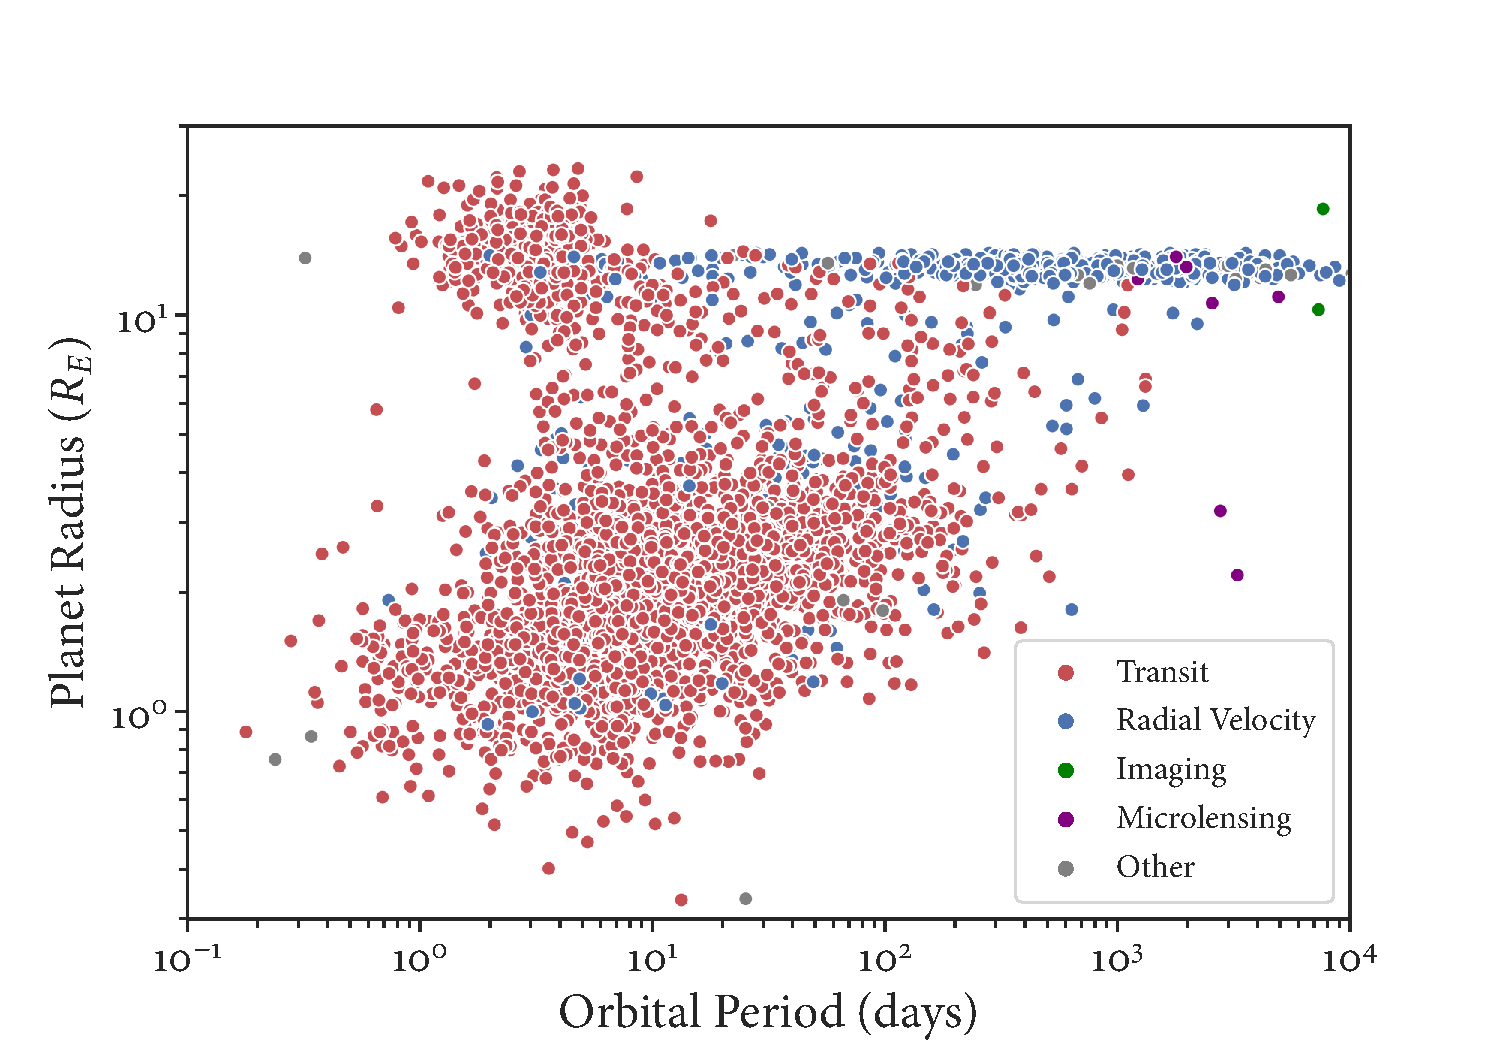
\includegraphics[width=1.0\textwidth]{figures/lit-review/planet-population.pdf}
    \caption{The population of known exoplanets plotted by planetary radius and orbital period, labelled by discovery method. The discovery methods are biased towards planets with particular properties.}\label{fig:review-planet-population}
\end{figure}


%SUBSECTION -- DISCOVERY
\subsection{Discovering Exoplanets}

Most exoplanets discovered to date have been found using either a ``radial velocity'' method or a ``transit'' method \citep{perryman2018exoplanet}. In the radial velocity (Doppler spectroscopy) method, the motion of a star around its common centre of mass with an orbiting planet is detected by measuring the Doppler-shift of emission lines of the star. The magnitude and period of this motion give the period of the planet's orbit, and a lower limit on its mass, owing to the degeneracy between the mass and the inclination in their effect on the signal.

In the transit method, an observer measures the reduction in flux from the star when the planet crosses the line of sight from the observer to the star (its ``primary transit''). The time between successive transits gives the orbital period of the planet, and the depth of the transit gives the radius of the planet at the wavelength observed. Combining the mass and period from a radial velocity measurement with the radius and period from a transit observation also gives the density and equilibrium temperature of the planet, which are vital for understanding planetary composition and important for atmospheric modelling.

Figure \ref{fig:review-planet-population} shows how different discovery methods are biased towards the detection of different types of planet. The red dots show planets discovered by the transit method, which are currently the most common due to the success of the \textit{Kepler} telescope. These planets are clustered to the left of the plot, as transits are more likely to be detected for close-in planets in short-period orbits, which reduce the flux from their star more strongly when they transit. The blue dots show planets detected by the radial velocity method, which produces stronger signals for higher-mass planets like the gas giants at the top of the plot.

The planets shown in green were detected by direct imaging, in which the light from their host star is blocked with a coronagraph and the planet is directly observed. This is currently only possible for young, large, self-luminous planets orbiting far from their star, so these planets are found to the top right of the plot. Direct imaging will become possible for more planets in the coming decade \citep{perryman2018exoplanet}.

%SUBSECTION -- CHARACTERISATION
\subsection{Characterising Exoplanets}

The atmospheres of exoplanets can be characterised with transmission and emission spectroscopy. Transmission spectroscopy measures the spectrum of light from the host star that passes through the atmosphere of the exoplanet as it transits. Measuring the depth of the transit at different wavelengths gives the radius of the planet and its atmosphere at those wavelengths, which depends on the opacity of the atmosphere. This allows the absorption spectrum of the gases in the atmosphere to be reconstructed, which can then be used to estimate the composition of the atmosphere \citep{tsiaras2016detection}.



Emission spectroscopy measures the spectrum of the thermal emission of the planet and its atmosphere. Hotter planets are better suited to this method as they emit more strongly at thermal wavelengths. The thermal emission depends on the composition of the atmosphere and its thermal structure, meaning that it can be used to reconstruct the vertical structure of the atmosphere \citep{stevenson2014thermal}.

Features of the atmospheric circulation of exoplanets are starting to be measured. The bulk wind speed of the atmosphere of an exoplanet can be measured via the Doppler-shift of absorption lines in its transmission spectrum \citep{louden2015spatially, brogi2016rotation}. Phase curve observations of the thermal emission of an exoplanet over its whole orbit have been used to infer the atmospheric circulation on hot Jupiters \citep{zellem2014hd209, parmentier2017handbook}, which I will discuss in more detail later.


%SECTION 2 -- TIDALLY LOCKED PLANETS
\section{Tidally Locked Planets}

An asynchronously rotating planet like the Earth has a different rotation period (1 day) to its orbital period (1 year). A synchronously rotating, or ``tidally locked'', planet has the same rotation period as its orbital period. This means that it always presents the same face to its host star, so it has a permanent day-side and a permanent night-side. I explained previously that planets orbiting close to their star are more likely to be detected, and are better suited to atmospheric characterisation. This section will show that these close-in planets are more likely to be tidally locked. This means that tidally locked planets should make up many of the best targets for atmospheric observations \citep{crossfield2015observations}.



%SUBSECTION -- DYNAMICS
\subsection{Formation}

All planets are affected by tidal stress due to their gravitational interaction with their host star. At the centre of mass of the planet, the gravitational force exactly balances the centrifugal force. The gravitational attraction is stronger than the centrifugal force for the part of the planet closest to the star, and the opposite is true for the part of the planet further from the star. This produces a stress that elongates the planet along the axis between it and the star. If the planet is not tidally locked, the long axis of the resulting ellipse will rotate away from this axis, and the stress will deform the planet further. This continual deformation removes rotational kinetic energy from the planet, until it reaches a tidally locked state where the long axis of the ellipsoid points towards the star permanently and no more energy is dissipated. Stable spin-orbit resonances are also possible, such as the 3:2 resonant orbit of Mercury, so not all planets affected by these stresses will reach a 1:1 tidally locked state.

The gravitational tidal stress acting on a planet is $\Sigma=2 G M_{*} / r^{3}$, where $M_{*}$ is the mass of the star and $r$ is the distance between the planet and the star \citep{pierrehumbert2018review}. The cubic dependence on $r$ makes the tidal locking timescale very sensitive to the semi-major axis. \citet{pierrehumbert2018review} estimate the time for a planet to become tidally locked to be:

\begin{equation}
  t_{\mathrm{lock}}=3.01 \times 10^{8} \frac{\rho \Omega_{0} r^{6}}{M_{*}^{2}} \frac{Q}{k_{2}},
\end{equation}

where $r$ is the mean orbital distance in AU, $\rho$ is the mean density of the planet in units of Earth density, and $\Omega$ is the angular velocity of the planet in units of Earth angular velocity. $Q$ corresponds to the effect of the dissipation of energy from tidal stresses \citep{goldreich1966q}, and $k_{2}$ is the Love number, which depends on the rigidity of the planet \citep{barnes2017tidal}. \citet{pierrehumbert2018review} use values for Earth and Venus to estimate the ratio for a generic terrestrial planet as $Q/k_{2} \approx 1000$.

 \citet{pierrehumbert2018review} use this formula to estimate that the rocky Earth-sized planet Trappist-1d would become tidally locked in 4000 years, assuming that it forms with the same initial angular velocity as Earth. By the same approximation, the super-Earth lava planet 55 Cancri e would take 6 years to reach this state. These short timescales suggest that the planets are very likely to be tidally locked. It is less clear whether planets with estimated tidal locking timescales of millions or billions of years will actually have reached this state.

\citet{leconte2015asynchronous} showed how atmospheric thermal tides oppose the gravitational tides discussed above, and slow the progress towards tidal locking. Thermal tides are caused by the thermal inertia of the atmosphere creating an excess of mass in the atmosphere  which lags behind the substellar point of an asynchronously rotating planet. The gravitational pull of the star on this mass excess produces a torque on the atmosphere, which acts on the planet in the opposite direction to the torque from the gravitational tide. Figure \ref{fig:review-leconte-tl} shows that this could inhibit tidal locking on Earth-mass planets. This effect would not be important for hot Jupiters, or the lava planets investigated in this thesis, but it is worth remembering that the simple estimate of a ``tidal locking timescale'' is not the whole story for many planets.

\begin{figure}
  \centering
  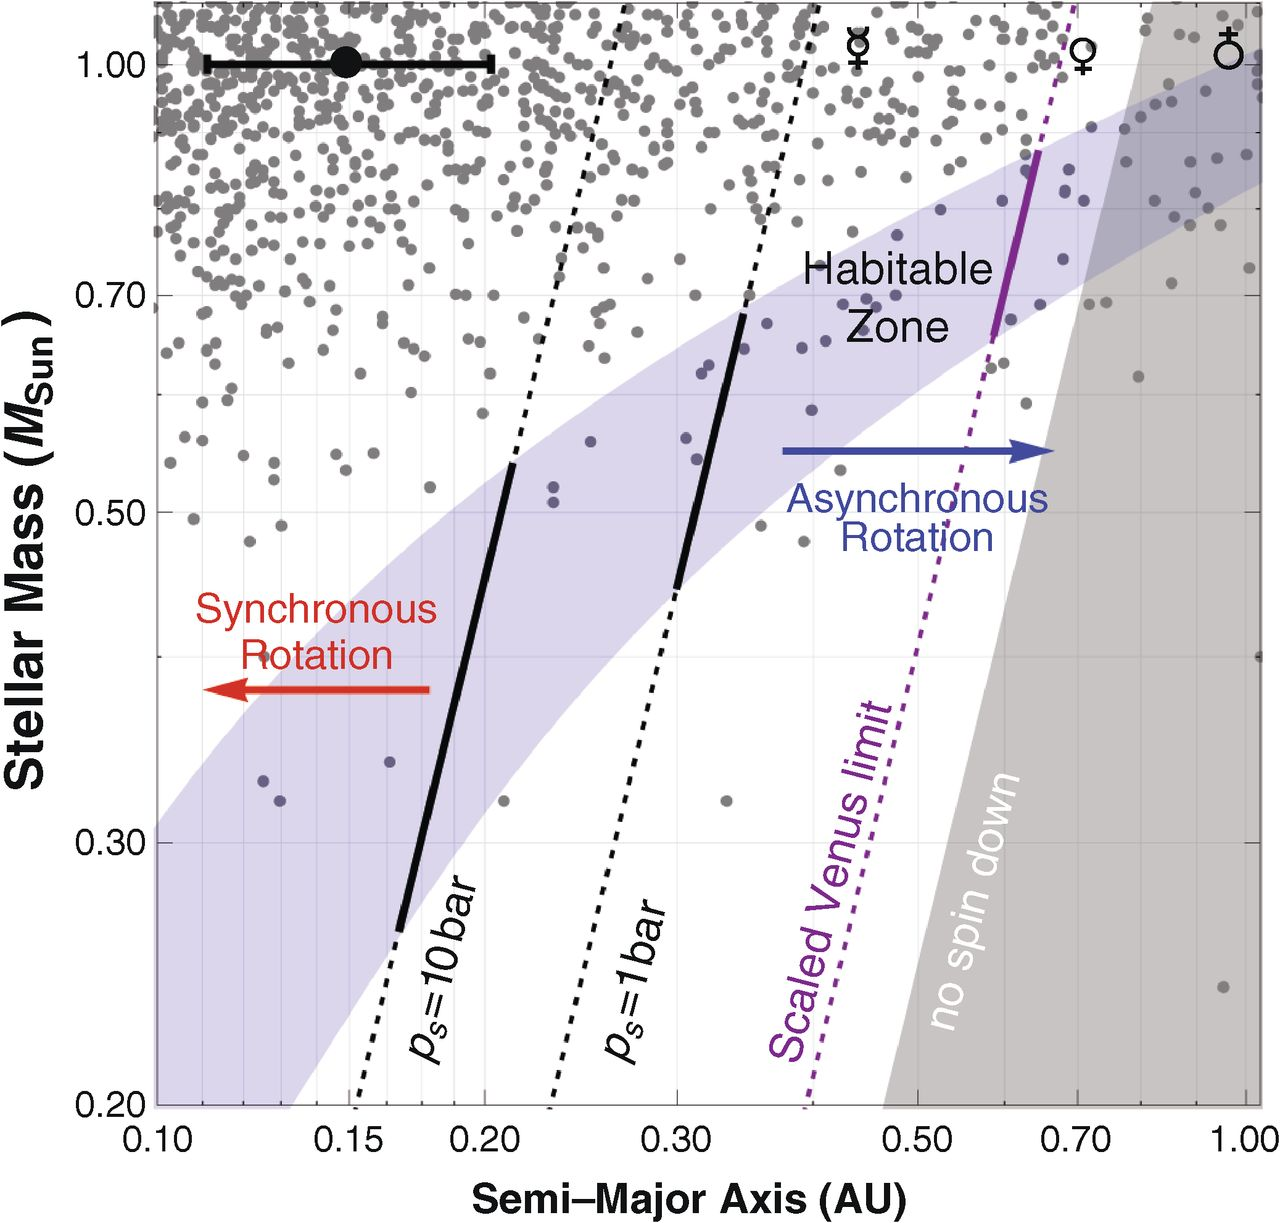
\includegraphics[width=0.6\textwidth]{figures/lit-review/leconte-tl.jpg}
\caption{A parameter space of stellar mass versus semi-major axis for discovered exoplanets, with lines showing the regions expected to have tidally locked planets with atmospheres of different thicknesses, from \citet{leconte2015asynchronous}. The thermal tide of the atmosphere may prevent Earth-like planets from become tidally locked.}\label{fig:review-leconte-tl}
\end{figure}


%SUBSECTION -- 55 Cancri system
\subsection{Lava Planets and 55 Cancri e}

Chapters \ref{ch:linking-climate-55cnce} and \ref{ch:clouds-lava-planets} investigate the atmospheric dynamics of ``lava planets''. These are hot rocky planets with a partially or fully molten surface, known as a ``magma ocean''. Lava planets are well suited to atmospheric observations due to their high temperatures and proximity to their stars, so are useful case studies for understanding the atmospheric dynamics of tidally locked planets.

55 Cancri e is the best-characterised example of a lava planet. It is a super-Earth with radius $1.95\ \mathrm{R_{E}}$ and orbital period 0.737 days \citep{crida201855cnce}. \citet{mcarthur2004detection} first detected the planet via the radial velocity method with an incorrect period of 2.808 days. \citet{dawson2010radial} showed that this period was due to spurious aliasing caused by gaps in the observations and corrected the period. It is expected to be tidally locked due to the short tidal locking timescale estimated above, and the observations of \citet{demory201655cnce}.

 % \citet{madhusudhan2012possible} used interior models constrained by mass and radius measurements of 55 Cancri e to suggest that its interior is carbon-rich. More recently, \citet{dorn2018new} suggested that it is one of a class of similar Super-Earths with a lower interior density than the Earth, with no core.

 \citet{demory201155cnce} and \citet{winn2011super} detected transits of the planet at infrared and visible wavelengths, opening the possibility of atmospheric characterisation.  \citet{demory2015variability} measured variable day-side thermal emission from 55 Cancri e over eight secondary eclipses, and suggested that this could be due to large-scale changes on the surface caused by strong tidal interactions with the star. \citet{tsiaras2016detection} reported the detection of an atmosphere with the WFC3 instrument on the Hubble Space Telescope, which appeared to be hydrogen-rich with a possible detection of HCN. The possibility of observing the composition of an atmosphere of the planet with emission spectroscopy has been explored by \citet{miguel2018observability} and \citet{ito2015theoretical}, who simulated a variety of spectra of potential atmospheres of different compositions and thicknesses.



%SUBSECTION -- PHASE CURVE
\subsection{A Thermal Phase Curve of 55 Cancri e}


\begin{figure}
  \centering
  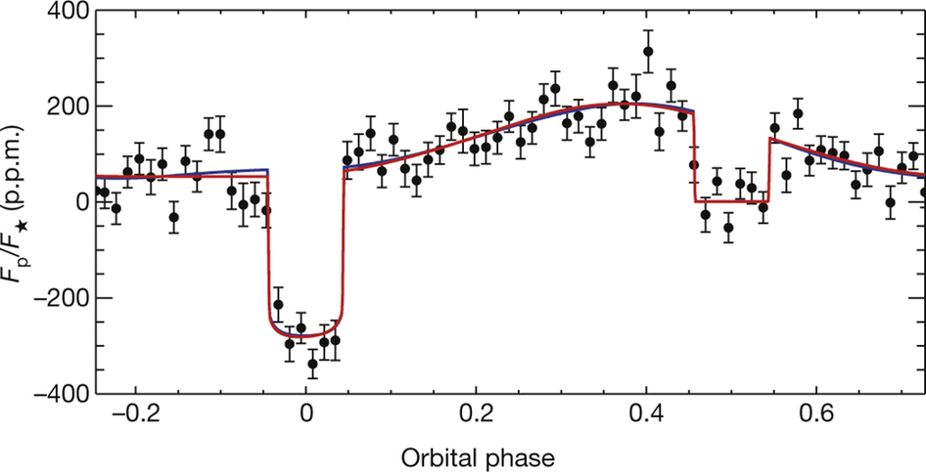
\includegraphics[width=0.7\textwidth]{figures/linking-climate-55cnce/demory-phase-curve.jpg}
\caption{The thermal phase curve observed in the \SI{4.5}{\micro\metre} \textit{Spitzer} bandpass by \citet{demory201655cnce}, showing an offset of the maximum flux from the secondary eclipse (the second dip), corresponding to a hot-spot shift possibly caused by atmospheric circulation. Reproduced from \citet{demory201655cnce} with permission.}\label{fig:review-demory-phase-curve}
\end{figure}


A ``phase curve'' is the radiation received from a planet over one complete orbit of its star. They contain information about how the emission or albedo of the planet varies with longitude, showing features such as day-night temperature differences. Phase curves measured at thermal wavelengths correspond to the radiating temperature of the planet or its atmosphere, so show features such as day-night temperature contrasts on tidally locked planets. Phase curves measured at optical wavelengths show the light from the host star reflected by the planet, so can show how the albedo of the planet varies due to heterogeneous features such as clouds \citep{parmentier2016transitions,parmentier2017handbook}. The phase curve has no latitudinal resolution, as the flux at any orbital phase only depends on the longitude at which the planet is observed. Techniques such as ``eclipse mapping'' can also retrieve latitudinal information, but require stronger emission from the planet \citep{majeau20122dmap}.

\begin{figure}
  \centering
  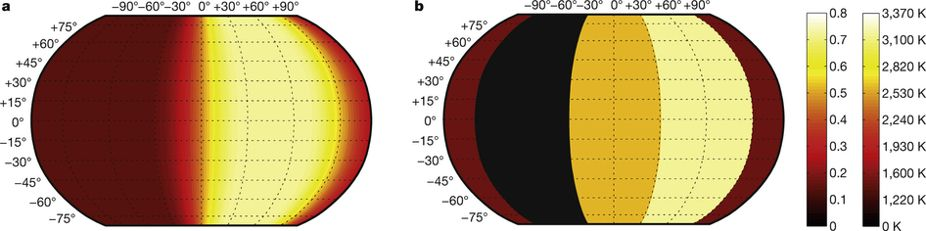
\includegraphics[width=0.95\textwidth]{figures/linking-climate-55cnce/demory-temp-maps.jpg}
\caption{The temperature map reconstructed by \citet{demory201655cnce} from the phase curve in Figure \ref{fig:demory-phase-curve}, showing a hot-spot shift of \ang{41}, a day-side temperature of \SI[separate-uncertainty = true]{2700(270)}{\kelvin}, and a night-side temperature of \SI[separate-uncertainty = true]{1380(400)}{\kelvin}. Reproduced from \citet{demory201655cnce} with permission.}\label{fig:review-demory-temp-maps}
\end{figure}

Phase curves are especially relevant to the atmospheric dynamics investigated in this thesis as the longitudinal variation of temperature on a planet can depend strongly on its global circulation. Figure \ref{fig:review-demory-phase-curve} shows the thermal phase curve of 55 Cancri e measured by \citet{demory201655cnce} using the \SI{4.5}{\micro\metre} channel of the \textit{Spitzer} space telescope. Figure \ref{fig:review-demory-temp-maps} shows the map of brightness temperature inferred from this phase curve. The phase curve implies a night-side temperature of \SI{1300}{\kelvin}, implying a significant warming of the night-side by atmospheric heat transport. It also shows a hot-spot shifted \SI{41}{\degree} east of the substellar point, which would be the hottest part without any atmospheric circulation. This hot-spot shift is similar to the phase shift in the optical phase curve measured by \citet{dragomir2012most} with the \textit{MOST} space telescope, which set an upper limit of 0.6 on its geometric albedo.

\citet{angelo201755cnce} analysed this phase curve using a similar 1D energy balance model to \citet{zhang2017dynamics}. They tuned the planetary Bond albedo, atmospheric surface pressure, heat redistribution efficiency, and greenhouse effect in this model, to match the observed phase curve. The parameters that fit best were a surface pressure of \SI{1.4}{\bar} and a heat redistribution efficiency of 1.47 (the ratio of radiative to advective timescales).

% The thermal phase curves of 55 Cancri e and other tidally locked planets motivated the work in this thesis to understand the atmospheric dynamics of tidally locked planets, and to simulate their observable consequences.



%SUBSECTION -- DYNAMICS
\section{Atmospheric Dynamics}

This section discusses current models of the dynamics of exoplanet atmospheres, and the theory of their global circulation. It introduces the concept of superrotation, which is a key part of the circulation of tidally locked planets.

\subsection{Numerical Atmospheric Models}

A General Circulation Model (GCM) is a three-dimensional fluid dynamical model of the atmosphere or the ocean of a planet, or both. They have been used to model the Earth, other planets in the Solar Systems, and are now used to simulate a wide variety of exoplanet atmospheres, often closely matching observations \citep{heng2015review, arcangeli2019climate}. GCMs typically consist of a dynamical core coupled to a representation of physical forcing such as radiative transfer or convective adjustment. The physics modelled in a GCM can range from very simple parameterisations capturing key processes \citep{held1994proposal} to highly detailed models of interacting clouds, radiative transfer, or other small-scale processes \citep{lines2018simulating, drummond2018observable}.

The GCM Exo-FMS used in this thesis based on the GFDL Flexible Modelling System\footnote{\url{gfdl.noaa.gov/fms/}} and the associated cubed-sphere dynamical core\footnote{\url{gfdl.noaa.gov/cubed-sphere-quickstart/}} \citep{ding2016convection, pierrehumbert2016dynamics, hammond2017climate, hammond2018wavemean}. Appendix \ref{ap:exo-fms} outlines the overall structure of the model, the dynamical core and associated grids, and the physics modules that can be swapped in and out of the model.

In the field of exoplanet studies, GCMs have perhaps been applied most successfully to modelling the atmospheres of hot Jupiters \citep{showman2002atmospheric, mayne2014unified, parmentier2016transitions, amundsen2016hd209, mayne2017hotjupiter}. Terrestrial planets have also been modelled to suggest potential circulation regimes or stable climate states \citep{merlis2010atmospheric, showman2012review, boutle2017proxima, noda2017circulation}. Other classes of exoplanet such as super-Earths or mini-Neptunes have been modelled in varying levels of detail \citep{carone2015regimes, charnay20153d, heng2015review}.


\subsection{Superrotation}\label{sec:superrotation}

Superrotation refers to a state where an atmosphere has more angular momentum than the solid planet below it. There are different ways of defining this mathematically -- I will use the definition of \citet{read1986super}, which defines superrotation as a positive ``superrotation index'', corresponding to an excess of atmospheric angular momentum over solid-body rotation at the equator. The local superrotation index is:

\begin{equation}
  s=\frac{m}{\Omega a^{2}}-1,
\end{equation}

where $\Omega$ is the planetary angular velocity, $a$ is the radius, and the specific angular momentum $m$ is:

\begin{equation}
 m=a \cos \phi(\Omega a \cos \phi+u),
\end{equation}

where $\phi$ is the latitude and $u$ is the local zonal velocity. An atmosphere with an ``ideal'' meridional circulation would homogenise the angular momentum of the equatorial surface in its upper branch, so the local superrotation index would be zero at all latitudes in that layer. The meridional circulation does not achieve this in reality (as on the Earth) and the superrotation index will be negative in most places \citep{read2018superrotation}. A process transporting angular momentum towards the equator, such as the stationary waves on tidally locked planets that produce an equatorial jet \citep{showman2011superrotation}, can produce an excess of angular momentum. This gives a positive local superrotation index at the equator.

The global superrotation index is a mass-weighted integral of the local superrotation index, and corresponds to a global measure of the magnitude of superrotation in the atmosphere:

\begin{equation}
  S_{m}=\frac{\iiint \rho m \mathrm{d} V}{\iiint \rho \Omega a^{2} \cos ^{2} \phi\ \mathrm{d} V}-1,
\end{equation}

where $\rho$ is the local density, and $\iiint \mathrm{d} V$ is an integral over the total volume of the atmosphere. Hide's Theorem states that the local $s$ and global $S_{m}$ cannot be positive anywhere without up-gradient angular momentum fluxes \citep{hide1969dynamics}. Superrotation is found in the atmosphere of Earth and other planets in the Solar System such as Venus and Titan \citep{laraia2015superrotation, read2018superrotation, sugimoto2019fully}. In this thesis, eastward angular momentum is transported towards the equators of tidally locked planetary atmospheres, producing a superrotating equatorial jet \citep{showman2011superrotation}.

\subsection{Dynamics of Tidally Locked Atmospheres}

The atmospheres of tidally locked planets are forced by their star in a very different way to the planets in the Solar System. The main source of atmospheric dynamics is the strong contrast in heating and cooling between the day-side and the night-side. This could be expected to drive an isotropic flow from the substellar point on the day-side to the antistellar point on the night-side, which can sometimes appear in simulations of very slowly rotating or strongly damped atmospheres \citep{pierrehumbert2018review, arcangeli2019climate}. In more realistic cases with faster rotation, the day-night forcing excites stationary waves that pump eastward momentum towards the equator, producing a superrotating jet that transports heat from the day-side to the night-side \citep{showman2011superrotation}. I will investigate the formation of this zonal flow in Chapter \ref{ch:eqm-zonal-flow}.

This equatorial superrotation was predicted by GCM simulations of terrestrial and gaseous tidally locked planets before its effects were observed \citep{joshi1997tidally, showman2002atmospheric}. These simulations predicted that the jet would shift the hottest part of the planet to the east of the substellar point, which was found to be true in thermal phase curves measured for many hot Jupiters \citep{parmentier2017handbook}. Figure \ref{fig:review-ar_mediumT_10day} shows a typical global temperature map from a simulation of a tidally locked planet, with the hot-spot shifted east of the substellar point. This shift was initially thought to be caused by pure advection of heat by the flow, but \citet{tsai2014three} showed that the eastward jet could shift the stationary waves excited by the day-night forcing eastwards, producing the hot-spot shift. \citet{perez2013atmospheric} also showed that the wave timescale is more important to this shift than the advective timescale of a hot Jupiter. I will discuss this in more detail in Chapter \ref{ch:wave-mean-flow}, and will show how a latitudinally sheared equatorial jet produces the global circulation pattern and hot-spot shift.

\begin{figure}
  \centering
  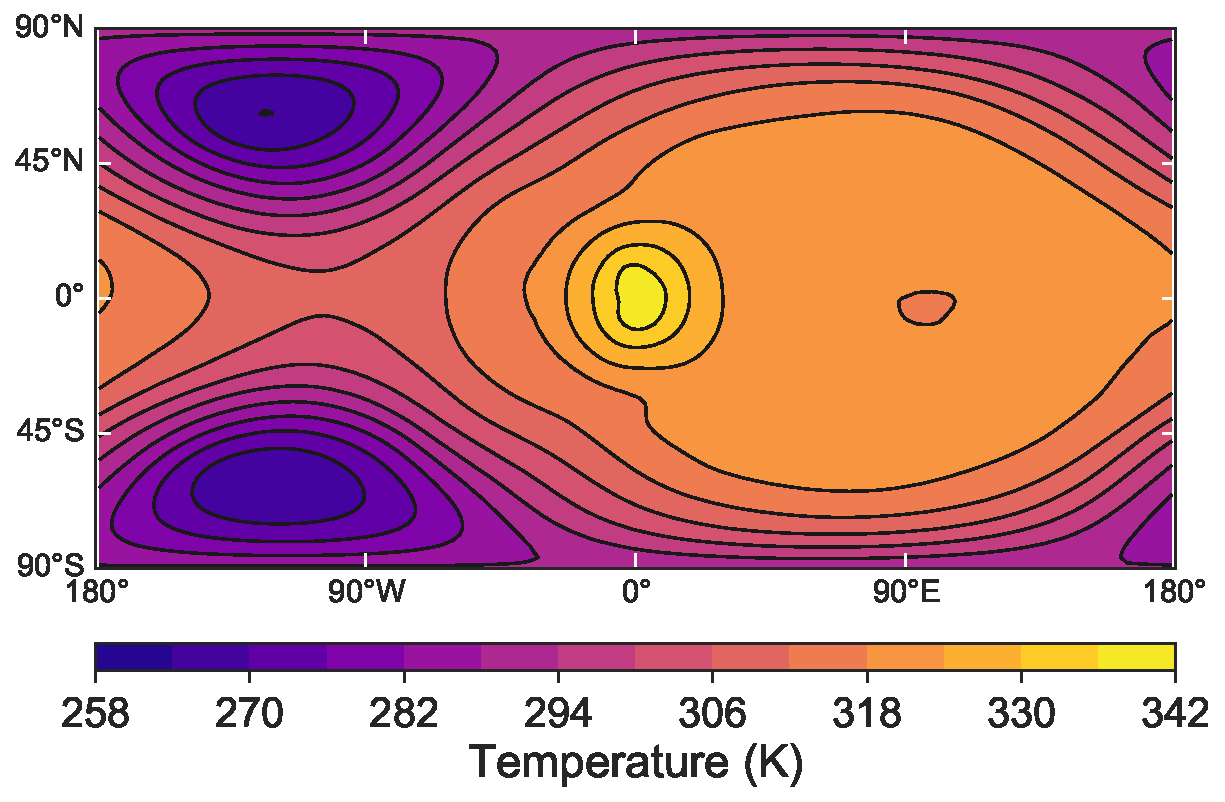
\includegraphics[width=0.65\textwidth]{figures/lit-review/ar_mediumT_10day.pdf}
\caption{The global temperature field at \SI{500}{\milli\bar} of a simulation of a tidally locked Earth-sized planet with a 10 day rotation period and a 1 bar N$_{2}$ atmosphere, showing an eastward shifted hot-spot and night-side cold stationary waves, reproduced from \citet{pierrehumbert2018review}.}\label{fig:review-ar_mediumT_10day}
\end{figure}


The formation of the superrotating jet is still not fully understood. Studies such as \citet{kataria2015atmospheric} compared real observations to the results of GCM simulations of tidally locked hot Jupiters, expecting that the global circulation formed by the GCM was reasonably accurate. However, \citet{thrastarson2010effects} suggested that simulations of the atmospheres of hot Jupiters depended strongly on initial conditions, and that the equilibrium states were not necessarily unique. \citet{liu2013atmospheric} suggested that this was not the case if a bottom drag was applied to the atmosphere, which they justified as an interaction with a deeper layer not represented in the GCM. Their simulations reached the same equilibrium state regardless of the initial conditions. However, \citet{cho2015sensitivity} demonstrated that the short timescale of this drag removed the variability otherwise present in the simulations, and concluded that while a bottom drag may remove sensitivity, it may also remove physically important processes from the atmosphere. \citet{polichtchouk2014intercomparison} further cast doubt on the results of other GCM simulations by showing significant differences between the results of different GCMs modelling the same exoplanets. More recent simulations such as \citet{mendoncca2016thor} have successfully modelled hot Jupiters without applying a bottom drag, suggesting that the earlier discrepancies may have been problems with the specific models. The question of the sensitivity to initial conditions and role of bottom drag is still not fully resolved, which motivates the investigation of the basic dynamics forming this global circulation in Chapter \ref{ch:eqm-zonal-flow}.

It is becoming possible to predict and test scaling relations of atmospheric circulation against observations of many exoplanets in a large parameter space. \citet{komacek2016daynightI}, \citet{komacek2017daynightII}, and \citet{zhang2017dynamics} used a 1D model balancing the advection of heat against radiation to model the circulation of a tidally locked planet. These models were used to explain scaling relations between the observed atmospheric circulation and the bulk composition and parameters of the atmosphere. Chapters \ref{ch:linking-climate-55cnce} and \ref{ch:clouds-lava-planets} will compare simulations of the atmospheric dynamics of the tidally locked planet 55 Cancri to observations of its temperature distribution, to constrain its potential atmospheric properties.












%%%%%%%%%%%%%%%%%%%%%%%%%%%%

%
% % 0 -- LEAD-IN PARAGRAPHS
%
% %START ELEMENT
% Perhaps the most exciting discovery from the field of exoplanet science is that other stars host planets which are very different from those in our solar system. There are similar planets to those in the solar system -- ``hot Jupiters'', high-temperature Jupiter-sized gas giants in short-period orbits, or ``Mini-Neptunes'', which show the literal-mindedness of planetary scientists. But some exoplanets have no analogues in the solar system, and ``lava planets'' are some of the best examples of these.
%
%
% %FRAMING TEXT
% This short chapter describes the class of ``lava planets'', particularly the planet 55 Cancri e, and discusses the question that this thesis aims to answers about this planet.
%
% %SIGNPOSTS
% I will describe lava planets in general, and list the known planets in this class. I will then discuss the 55 Cancri system, and the lava planet 55 Cancri e in that system.
%
% %SUMMARISE CONCLUSIONS
% I will try to show that lava planets are a potentially bountiful area for scientific work, being interesting systems that have observational advantages. I will set up the question of the atmosphere and atmospheric circulation of 55 Cancri e, and show how it relates to the broader question of the nature of the climate of tidally locked planets.
%
%
% %SECTION 1 -- EXOPLANETS
% \section{Exoplanets}
%
% Exoplanets are planets orbiting stars other than our Sun. As far as we know, there is nothing fundamental to distingush the planets in our Solar System from those elsewhere, so it is possible that this specific nomenclature may eventually disappear. I will use the word ``exoplanet''  when discussing specific planets or issues related to their distance, and ``planet'' in a more general or idealised context (such as the first sentence of this paragraph).
%
% There is no better way to date a piece of writing on exoplanets than by announcing how many have been discovered, so I will just note that we know of several thousand and anticipate many more to come. The number of exoplanets which are favourable for detailed observations is still quite small, and we can observe atmospheric details for perhaps only a few dozen planets. In fact, while the title of this thesis suggests it looks at ``lava planets'', there is really only one that is currently observable -- 55 Cancri e. Despite this, I hope to draw general conclusions about the circulation of many types of planet, and contribute to an understanding of tidally locked planets and lava planets for future observations.
%
%
% %SUBSECTION -- DISCOVERY
% \subsection{Discovering Exoplanets}
%
% This is not a thesis on discovering exoplanets, although the methods of discovery are sometimes relevant to the characterisation that is of interest. Most exoplanets discovered to date have been found using either a ``radial velocity`` method or a ``transit'' method.
%
% In the first method, the motion of a star around its common center of mass with a planet orbiting it is detected by measuring the Doppler-shift of emission lines of the star. The magnitude and period of this motion gives the period of the planet's orbit, and a limit on its mass.
%
% In the second method, a planet passing across the line of sight from an observer to the star produces a dip in the light seen by the observer. A periodic dip gives the period of the planet, and the size of the dip gives its radius. So, if a planet can be measured with both methods the observer retrieves its period, mass, radius, density, semi-major axis, and equilibrium temperature.
%
%
% %SUBSECTION -- CHARACTERISATION
% \subsection{Characterising Exoplanets}
%
% This is also not a thesis on characterising exoplanets, although I have tried to keep observations in mind throughout the simulations and theory.
%
% The atmospheres of exoplanets can be characterised through transmission and emission spectroscopy. In transmission spectroscopy, light from the host star passes through the atmosphere of the exoplanet before it reaches the observer, and the spectrum is measured. An alternative (but equivalent) view is that the planet appears to have a different radius as it transits its star at different wavelengths -- at a wavelength the atmosphere is more opaque to, the planet appears larger -- so the absorption spectrum of the gases in the atmosphere can be retrieved.
%
% In emission spectroscopy, the spectrum of the light emitted thermally by the planet and its atmosphere is measured. Hotter planets emit more light in this way, so are better suited to this method.
%
% %SECTION CONCLUSIONS
%
%
%
%
% %SECTION 2 -- LAVA PLANETS
% \section{Lava Planets}
%
% %SUBSECTION --
% \subsection{Tidally Locked Planets}
%
% A tidally locked planet, or a ``synchronously rotating'' planet, always presents the same face to the star it orbits, as its rotation period is the same as its orbital period. An asynchronously rotating planet like the Earth has a different rotation period (1 day) to its orbital period (1 year). Tidal forces slow down the rotation of such planets, until they become tidally locked. The time for a planet to become tidally locked is approximately:
%
%
% See Chapter \ref{ch:wave-mean-flow} for an investigation of the atmospheric dynamics of tidally locked planets.
%
% Tidally locked planets include Hot Jupiters, Earth-like planets like those in the Trappist-1 system, and lava planets like 55 Cancri e, discussed next.
%
% %SUBSECTION --
% \subsection{The Atmospheric Circulation of Tidally Locked Planets}
%
%
%
% %SUBSECTION --
% \subsection{Lava Planets}
%
% ``Lava Planets'' are terrestrial (rocky, not gaseous) planets orbiting very close to their parent star.
%
% %SECTION CONCLUSIONS
%
% %SECTION 3 -- 55 CANCRI E
% \section{55 Cancri e}
%
% 55 Cancri e is a tidally locked lava planet orbiting the binary star 55 Cancri, 41 light years away in the constellation of Cancer.
%
% %SUBSECTION -- 55 Cancri system
% \subsection{The 55 Cancri system}
%
% Figure X shows the 55 Cancri system.
%
% %SUBSECTION -- 55 Cancri e
% \subsection{55 Cancri e}
%
% 55 Cancri e is the closest planet to the G-star 55 Cancri A.
%
% %SUBSECTION -- PHASE CURVE
% \subsection{A Thermal Phase Curve of 55 Cancri e}
%
% A phase curve is the light measured from a planet as it orbits its star. They are particularly useful for tidally locked planets. Figure X shows a phase curve for X.
%
% A thermal phase curve refers to the light emitted by the planet itself, rather than the light it reflects from the star it orbits. For a tidally locked planet, the thermal phase curve shows the hemisphere-averaged brightness temperature of the planet as it rotates.
%
% \citet{demory201655cnce} measured a thermal phase curve of the planet 55 Cancri e.
%
%
%
% %CONCLUSIONS
%
% 55 Cancri e is currently the most easily observable terrestrial tidally locked planet. Its composition, atmosphere, and circulation provide tests of theories of planet formation and atmospheric dynamics. In this thesis, I will use it as a case study for the atmospheric dynamics of tidally locked planets.
%
% %RESTATE SECTION CONCLUSIONS
%
% %OPEN OUT CONCLUSIONS

% \bibliographystyle{unsrtnat}
% \bibliography{../references.bib}

 \begin{SingleSpace}
\chapter{The Gierasch-Rossow-Williams Mechanism on Tidally Locked Planets}\label{ch:eqm-zonal-flow}
% \vspace{0.5cm}
% \chapterprecishere{``One might as well approximate the derivatives well instead of badly''\par\raggedleft--- \textup{John P. Boyd}, Chebyshev and Fourier Spectral Methods}
\end{SingleSpace}
% \vspace{0.5cm}





%%%%%%%%%%%%%%%%%%%%%%%%%%%%
% 0 -- LEAD-IN PARAGRAPHS

%START ELEMENT

% ADD MOTIVATION FROM CHO/SHOWMAN DISPUTE

% NB PEREZ-BECKER AND SHOWMAN FORCING FIELD

The global atmospheric circulation of tidally locked planets is driven by day-side heating and night-side cooling. This forcing drives a flow from the day-side atmosphere to the night-side. The flow normally takes the form of single, or multiple, eastward zonal jets. This flow is of primary importance to the temperature distribution, observable features, and climate stability of these planets \citep{stevenson2014thermal,louden2015spatially,pierrehumbert2018review}.

%FRAMING TEXT

 \citet{showman2011superrotation} used a linear shallow-water model to represent the atmosphere of a tidally locked planet, showing that equatorward momentum transport produces the eastward jet \citep{matsuno1966quasi}. This linear model requires westward flow at high latitudes to conserve angular momentum when an eastward jet forms on the equator. However, GCM simulations often have eastward flow at all latitudes at the level of their equatorial jet, which is inconsistent with the linear model \citep{showman2015circulation,kataria2015atmospheric,pierrehumbert2018review}.

%SIGNPOSTS

This chapter uses the Gierasch-Rossow-Williams (GRW) mechanism to describe the formation of the zonal flow on tidally locked planets, and to explain the eastward flow at all latitudes seen in GCM simulations. This mechanism has been used to explain the formation of zonal flow on Venus and Titan \citep{gierasch1975meridional, rossow1979large, read2018superrotation}. The GRW mechanism combines a mean meridional circulation with an equatorward momentum transport, to produce the equatorial jet while accelerating subtropical jets at high latitudes.

I will recreate this mechanism in linear and non-linear shallow-water models, and show how the effect of the meridional circulation on a tidally locked planet can be approximated by its zonal mean only. I will show that the momentum fluxes governing the equilibrium flow in the shallow-water models are the same as those produced by GCM simulations. The balance of fluxes will predict scaling relations for the relative strengths and directions of the equatorial and high-latitude flow. I will conclude that the new mechanism requires sub-rotating flow at high latitudes -- which can be eastward or westward -- rather than the westward flow required by the linear model of \citet{showman2011superrotation}.

% I will show how combining the shallow-water model with the Gierasch-Rossow-Williams (GRW) mechanism gives a coherent description of the zonal flow in the GCM simulations. The GRW mechanism combines transport of angular momentum by a mean meridional circulation with equatorward transport by eddies, producing a superrotating flow at the equator. This means that a superrotating equatorial jet requires subrotating flow at higher latitudes, but this subrotating flow can still be westerly -- unlike the model in \citet{showman2011superrotation}, which requires easterly flow at high latitudes. This mechanism is therefore consistent with the westerly flow seen at all latitudes in some GCM simulations.
%
% The mean meridional circulation required for this mechanism is more complex on tidally locked planets, as their equator-to-pole-forcing gradient varies with longitude. However, I will show how to lowest order only the zonal mean of the forcing matters for the mean meridional circulation, so its effect can be easily approximated on a tidally locked planet. I will discuss the balance of sources of momentum transport giving zonal acceleration in GCM simulations and in a non-linear shallow-water model, and show  that the equilibrium zonal flow is governed by different balances at the equator and at high latitudes. Finally, I will use this mechanism to predict scaling relations for jet positions and speeds in both models, and will test these predictions against a suite of tests in the models.

%SUMMARISE CONCLUSIONS

% I will conclude that the formation of zonal flow on a tidally locked planet can be explained by the GRW mechanism, with equatorward momentum transport provided by the process explained in \citet{showman2011superrotation}. I will show that the balance of acceleration due to different momentum transports in this mechanism is the same in a linear shallow-water model, a non-linear shallow-water model, and a GCM. In the following chaper, I will use this understanding of the formation of zonal flow to describe its effect on the global circulation and temperature distribution.



%%%%%%%%%%%%%%%%%%%%%%%%%%%%
%SECTION 1 -- MATSUNO MODEL

\section{Linear Shallow-Water Model of a Tidally Locked Atmosphere}\label{sec:lin-sw-model}

This section reviews the linear shallow-water model used by \citet{matsuno1966quasi} to model equatorial waves in the Earth's tropics. I will show how \citet{showman2011superrotation} used this model to explain the formation of equatorial superrotation in tidally locked planetary atmospheres.

%SUBSECTION -- SW EQUATIONS
\subsection{Linear Shallow-Water Equations}

\citet{matsuno1966quasi} constructs a single-layer shallow-water model representing a single layer of fluid with a free upper surface on an equatorial beta-plane:

\begin{equation}\label{eqn:sw-eqns-1}
  \begin{gathered}
     \frac{\partial u}{\partial t} - \beta y v +\frac{\partial h}{\partial x} = 0, \\
      \frac{\partial v}{\partial t} + \beta y u + \frac{\partial h}{\partial y} = 0, \\
    \frac{\partial h}{\partial t} +c^{2}(\frac{\partial u}{\partial x} + \frac{\partial v}{\partial y}) =0, \\
  \end{gathered}
\end{equation}

where $u$ is the zonal velocity, $v$ is the meridional velocity, $h$ is the height, $t$ is time, and $c = \sqrt{gH}$ is the gravity wave speed. The ``beta-plane'' approximates the Coriolis parameter as $f=\beta y$, where $\beta$ is the ``Rossby parameter'' and $y$ is the meridional coordinate. Appendix \ref{ap:ps-methods} describes the pseudo-spectral method used to solve these equations.

Non-dimensionalising with time scale $\sqrt{1/c \beta}$ and length scale $\sqrt{c/\beta}$ (the equatorial Rossby radius of deformation $L_{R}$), and assuming all quantities have the form $f(y) e^{i( k x-\omega t)}$, the equations describing free perturbations are:

\begin{equation}\label{eqn:sw-eqns-2}
  \begin{gathered}
      - i \omega u - y v + i k_{x} h = 0, \\
      - i \omega v + y u + \frac{\partial h}{\partial y} = 0, \\
      - i \omega h + i k u + \frac{\partial v}{\partial y} = 0. \\
  \end{gathered}
\end{equation}

\citet{matsuno1966quasi} solves these equations analytically to find the dispersion relation of the free modes, and discusses the latitudinal structure of each mode. This chapter focuses on the response to stationary forcing rather than the free modes, but understanding their behaviour is important as their structures and eigenfrequencies will determine their magnitudes and positions in the forced response. The free modes could also be important to the time-variable behaviour of the atmosphere.


% Figure \ref{fig:disp-beta} shows the dispersion relation of the lower-order modes.


% \begin{figure}
%   \centering
%   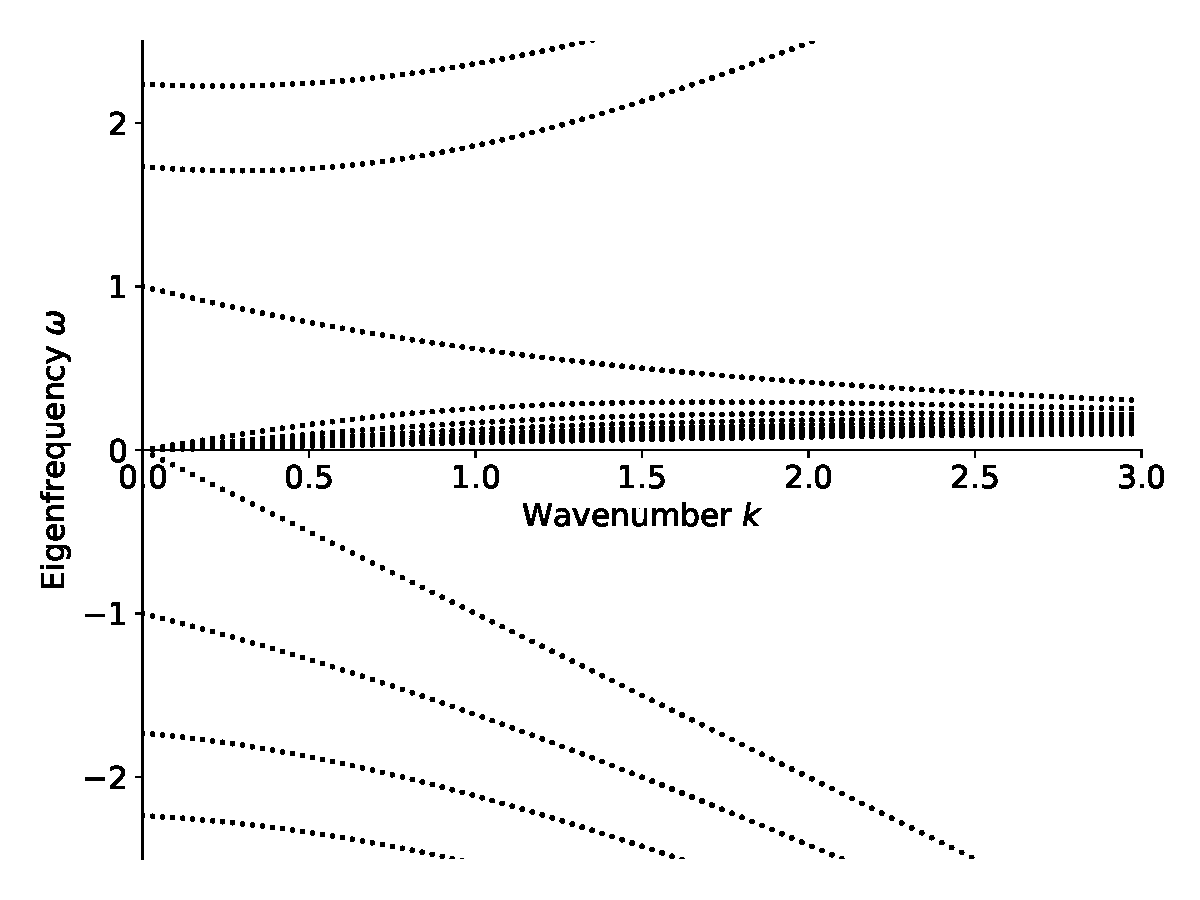
\includegraphics[width=0.7\textwidth]{figures/eqm-zonal-flow/disp-beta.pdf}
%   \caption{Dispersion relation on the beta-plane, calculated with spectral method giving the same results as the analytic solutions of \citet{matsuno1966quasi}.}
%   \label{fig:disp-beta}
% \end{figure}


The wave-1 forcing on a tidally locked planet is stationary and symmetric about the equator, so it will preferentially excite the lowest-order symmetric modes -- the Rossby and Kelvin modes. Figure \ref{fig:beta-plane-free-rossby} shows the free Rossby mode with zonal wavenumber 1. Its positive eigenvalue $\omega$ means that the free Rossby mode travels westwards (following the convention in \citet{matsuno1966quasi} for the relation between eigenvalue and direction of travel). Figure \ref{beta-plane-free-kelvin} shows the free Kelvin mode with zonal wavenumber 1. This is a special solution of the equations with zero meridional velocity, which has a negative eigenvalue so travels eastward as a free wave.

\begin{figure}
  \centering
  \begin{subfigure}[t]{0.49\textwidth}
    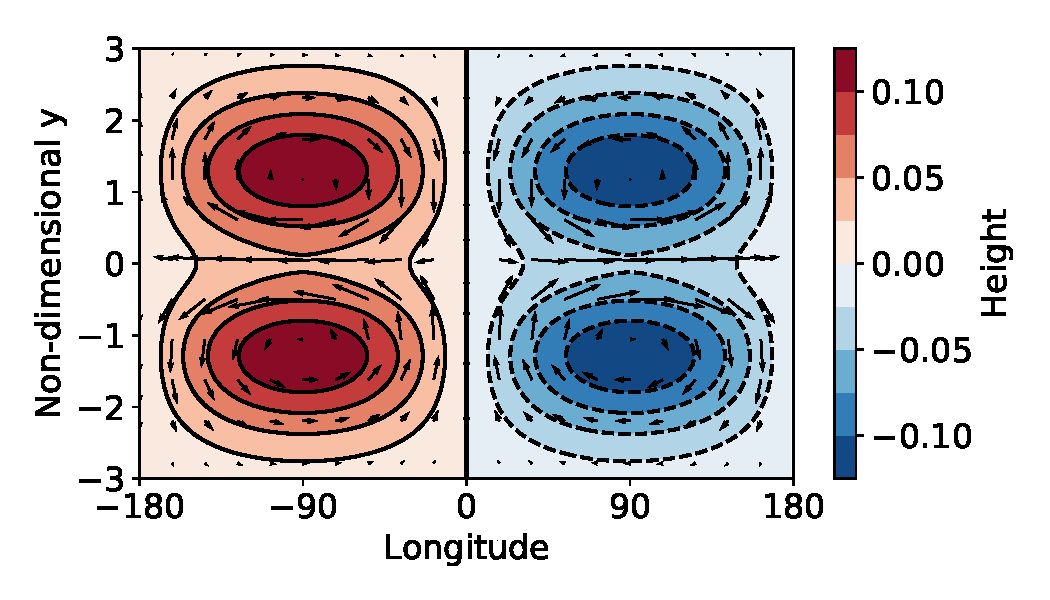
\includegraphics[width=1.0\textwidth]{figures/eqm-zonal-flow/beta-plane-free-rossby.pdf}
    \caption{Rossby wave.}
    \label{fig:beta-plane-free-rossby}
  \end{subfigure}
  %
  \begin{subfigure}[t]{0.49\textwidth}
    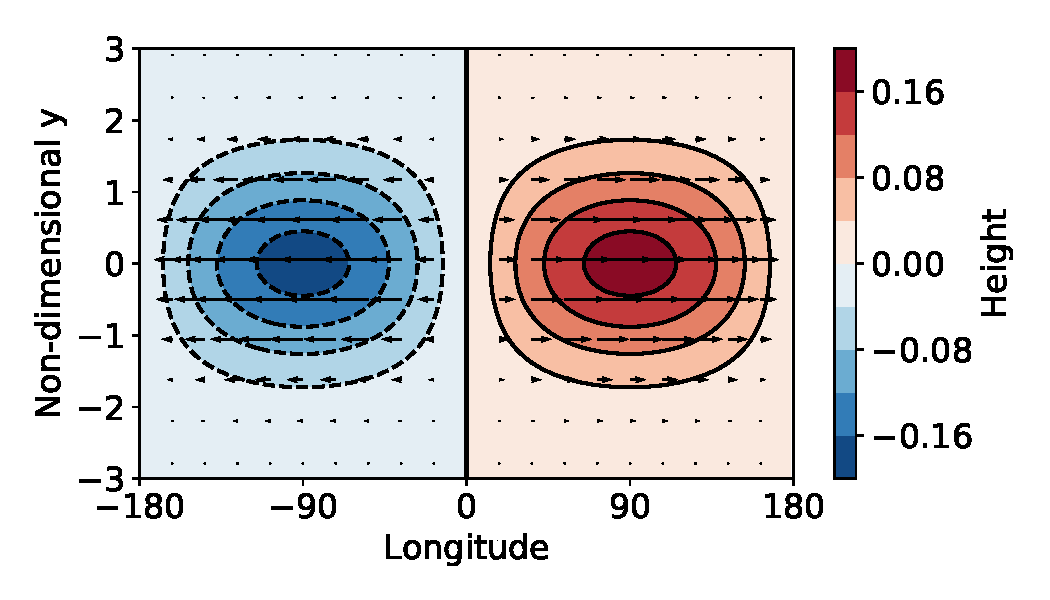
\includegraphics[width=1.0\textwidth]{figures/eqm-zonal-flow/beta-plane-free-kelvin.pdf}
    \caption{Kelvin wave.}
    \label{beta-plane-free-kelvin}
  \end{subfigure}
  \caption{The non-dimensional height and velocity fields of the lowest order free modes of a shallow-water system on an equatorial beta-plane. The response to forcing on a tidally locked planet is composed mainly of forced Rossby and Kelvin modes.}
  \label{fig:beta-plane-free-rossby-kelvin}
\end{figure}


%SUBSECTION -- RESPONSE TO FORCING
\subsection{Linear Response to Forcing}

\citet{showman2011superrotation} use this linear shallow-water model to represent the atmosphere of a tidally locked planet. A tidally locked planet is constantly heated on its day-side and cooled on its night-side, giving a stationary forcing very similar  to the forcing used in \citet{matsuno1966quasi}. This forcing $Q(x,y)$ acts on the $h$ field, giving the equations:

\begin{equation}\label{eqn:sw-eqns-forced}
  \begin{gathered}
    \alpha_{dyn} u - \beta y v +\frac{\partial h}{\partial x} = 0, \\
    \alpha_{dyn} v + \beta y u + \frac{\partial h}{\partial y} = 0, \\
    \alpha_{rad} h + c^{2}(\frac{\partial u}{\partial x} + \frac{\partial v}{\partial y}) = Q(x,y), \\
  \end{gathered}
\end{equation}

where both the dynamical and radiative damping rates $\alpha_{dyn}$ and $\alpha_{rad}$ are often set to a uniform damping $\alpha$ for a simpler solution. The boundary conditions are

\begin{equation}
  u , v , h \rightarrow 0 \quad \mathrm{for} \quad y \rightarrow \pm \infty.
\end{equation}

\citet{matsuno1966quasi} shows how the response of Equation \ref{eqn:sw-eqns-forced} to a forcing $Q(x,y) = Q_{0} \sin(x) e^{-y^{2}/2}$ and uniform damping $\alpha_{rad}=\alpha_{dyn}=\alpha$ can be found analytically as a sum of the free modes of the system.

The forced response $\chi = (u,v,h)$ is a sum of the free modes $\xi_{m}=(u_{m},v_{m},h_{m})$, weighted by coefficients $a_{m}$:

\begin{equation}
  \chi = \sum a _ { m } \xi _ { m },
\end{equation}

where the coefficients are

\begin{equation}
  a _ { m } = \frac { 1 } { \alpha - i \omega _ { m } } b _ { m },
\end{equation}

where $\omega_{m}$ is the eigenvalue of the mode $m$, and the projection of each mode onto the forcing is

\begin{equation}
  b _ { m } = \left[ \int \overline { \xi } _ { m } ( y ) \sigma ( y ) d y \right] / \left[ \int \left| \xi _ { m } ( y ) \right| ^ { 2 } d y \right].
\end{equation}

Figure \ref{fig:beta-plane-forced} shows the response to the forcing $Q(x,y) = Q_{0} \sin(x) e^{-y^{2}/2}$, where all the coefficients $a_{m}$ are zero apart from the Kelvin wave and $n=1$ Rossby wave. The Rossby wave appears west of the substellar point due to its positive eigenvalue $\omega_{m}$, and the Kelvin wave appears east of the substellar point due to its negative eigenvalue.

\begin{figure}
  \centering
  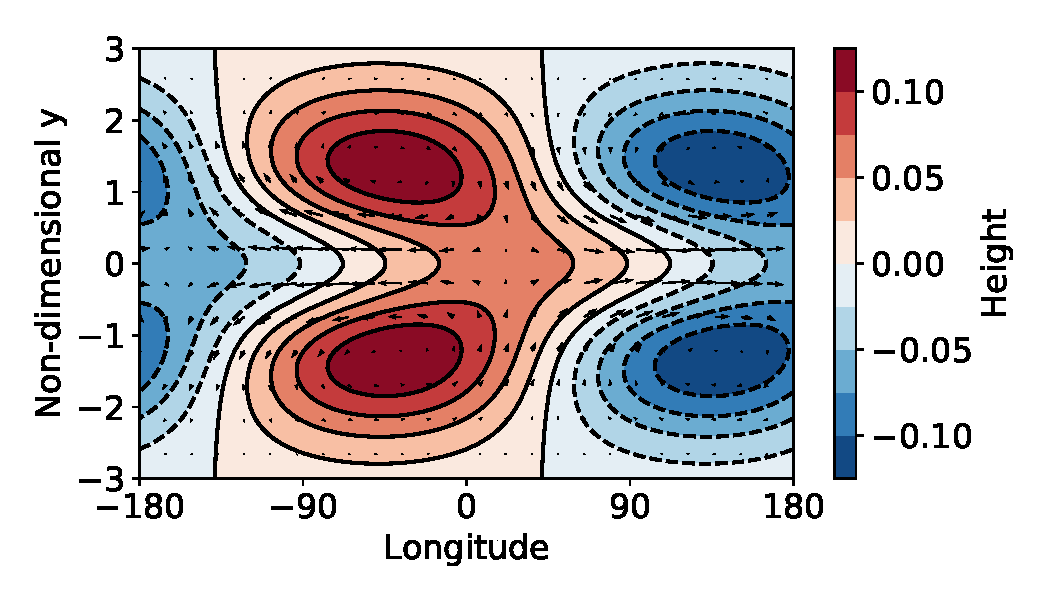
\includegraphics[width=0.65\textwidth]{figures/eqm-zonal-flow/beta-plane-forced.pdf}
  \caption{Non-dimensional response of Equation \ref{eqn:sw-eqns-forced} to forcing $Q(x,y) = Q_{0} \sin(x) e^{-y^{2}/2}$, showing the maximum of the Rossby wave west of the maximum of the forcing (the substellar point) and the maximum of the Kelvin wave east of this point.}\label{fig:beta-plane-forced}
\end{figure}


%SUBSECTION -- ACCELERATION
\subsection{Equatorial Acceleration}

The phase shift between the Rossby and Kelvin waves in the response to forcing produces an equatorward momentum transport that would be expected to produce equatorial superrotation \citep{showman2011superrotation, tsai2014three}. Zonally averaging the zonal momentum equation in Equation \ref{eqn:sw-eqns-1} gives the latitudinal acceleration profile \citep{thuburn1999zonalmean}:

\begin{equation}\label{eqn:zonal-mean-mom-no-R}
  \frac { \partial \overline { u } } { \partial t } = \underbrace { \overline { v } ^ { * } \left[ f - \frac { \partial \overline { u } } { \partial y } \right] } _ { I } \underbrace { - \frac { 1 } { \overline { h } } \frac { \partial } { \partial y } \left[ \overline { ( h v ) ^ { \prime } u ^ { \prime } } \right] } _ { I I } + \underbrace {  \frac { 1 } { \overline { h } } \overline { u ^ { \prime } Q ^ { \prime } } } _ { I I I } \underbrace { - \frac { \overline { u } ^ { * } } { \tau _ { \mathrm { drag } } } } _ { I V } - \frac { 1 } { \overline { h } } \frac { \partial \left( \overline { h ^ { \prime } u ^ { \prime } } \right) } { \partial t },
\end{equation}

where for a variable $X$, $\overline{X}^{*} = \overline{h X} / \overline{h}$. Figure \ref{fig:beta-fluxes-no-R} plots the terms in Equation \ref{eqn:zonal-mean-mom-no-R} for the response to forcing in Figure \ref{fig:beta-plane-forced}. It shows that the horizontal convergence of eastward momentum at the equator due to stationary eddies (term II) is exactly cancelled by the removal of eastward momentum from the equator by vertical momentum transport (term III). This means that the forced linear shallow-water model of \citet{matsuno1966quasi} does not accelerate at the equator, so a modification is needed to model the atmosphere of a tidally locked planet.

\begin{figure}
  \centering
  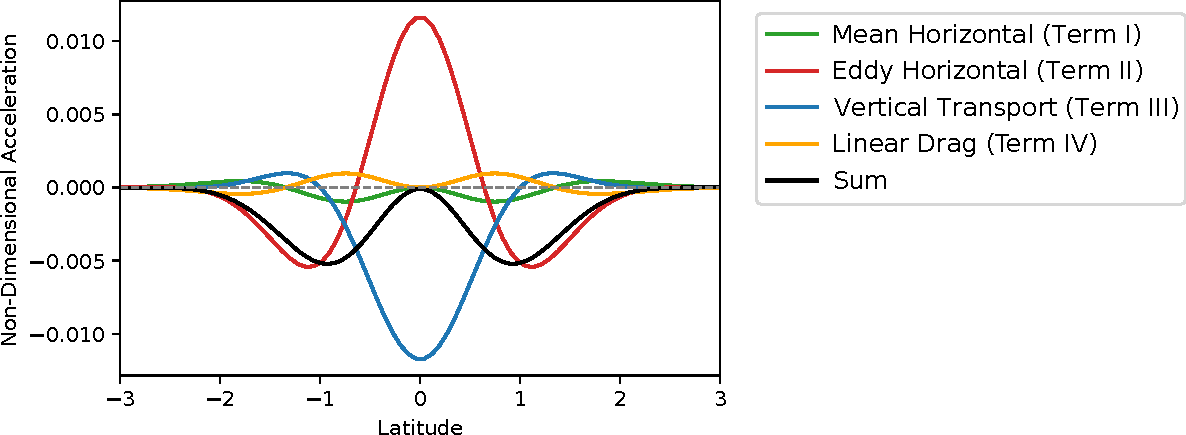
\includegraphics[width=1.0\textwidth]{figures/eqm-zonal-flow/beta-fluxes-no-R.pdf}
  \caption{Terms in the zonal-mean zonal momentum equation (Equation \ref{eqn:zonal-mean-mom-no-R}) without the correction $R$ to the momentum. The acceleration terms cancel exactly at the equator, which is why \citet{showman2010superrotation} introduced the correction $R$ to explain the formation of superrotation on tidally locked planets.}
  \label{fig:beta-fluxes-no-R}
\end{figure}

This can be explained by rewriting Equation \ref{eqn:zonal-mean-mom-no-R} in terms of the relative vorticity $\vec{\zeta}=\left(v_{x}-u_{y}\right) \hat{k}$ \citep{showman2011superrotation}:

\begin{equation}\label{eqn:zonal-mean-mom-zeta-no-R}
  \frac{\partial \overline{u}}{\partial t}=\overline{v^{\prime} \zeta^{\prime}}+\overline{v}(f+\overline{\zeta})-\frac{\overline{u}}{\tau_{\mathrm{drag}}},
\end{equation}

For forcing that is symmetric about the equator, the solutions are symmetric about the equator in $u$ and antisymmetric in $v$, so are also antisymmetric in $\zeta$. $v$ and $\zeta$ are therefore zero at the equator, so the first two terms in Equation \ref{eqn:zonal-mean-mom-zeta-no-R} are zero. This results in zero acceleration at the equator, for an atmosphere at rest with $\overline{u} = 0$.

\citet{showman2010superrotation} resolved this problem by introducing a correction $R$ to the mean vertical momentum transport. The correction represents the effect of advection between the active upper layer and quiescent lower layer \citep{shell2004superrotation}. \citet{showman2010superrotation} explain:

\textit{``Air moving out of the upper layer ($Q<0$) does not locally affect the upper layer’s specific angular momentum or wind speed, hence $R=0$ for that case. But air transported into the upper layer carries lower‐layer momentum with it and thus alters the local specific angular momentum and zonal wind in the upper layer.''}

Following \citet{shell2004superrotation}, they impose conservation of momentum between the stationary lower layer and the active upper layer, resulting in the correction:

\begin{equation}
  \mathbf{R}(\lambda, \phi, t)=\left\{\begin{array}{ll}{-\frac{Q \mathbf{v}}{h},} & {Q>0} \\ {0,} & {Q<0}\end{array}\right.
\end{equation}

\citet{shell2004superrotation} consider an axisymmetric planet where the air is rising at the equator and falling at the poles. In the tidally locked case, the air is rising at the substellar point and falling at the antistellar point. Figure \ref{fig:beta-plane-forced} shows that this term produces a net westerly acceleration at the equator. On the day-side where $Q>0$, the equatorial winds are mostly easterly, so $R$ is non-zero and positive, giving a westerly acceleration. On the night-side, $Q<0$ so there is no effect from $R$. This asymmetry in $R$ produces a net westerly acceleration at the equator.

Including the correction $R$, the zonal-mean momentum equation becomes:

\begin{equation}\label{eqn:zonal-mean-mom}
  \frac { \partial \overline { u } } { \partial t } = \underbrace { \overline { v } ^ { * } \left[ f - \frac { \partial \overline { u } } { \partial y } \right] } _ { I } \underbrace { - \frac { 1 } { \overline { h } } \frac { \partial } { \partial y } \left[ \overline { ( h v ) ^ { \prime } u ^ { \prime } } \right] } _ { I I } +\underbrace{\left[\frac{1}{\overline{h}} \overline{u^{\prime} Q^{\prime}}+\overline{R_{u}}^{*}\right]}_{\text { III }} \underbrace { - \frac { \overline { u } ^ { * } } { \tau _ { \mathrm { drag } } } } _ { I V } - \frac { 1 } { \overline { h } } \frac { \partial \left( \overline { h ^ { \prime } u ^ { \prime } } \right) } { \partial t },
\end{equation}

and in vorticity form, it is:

\begin{equation}\label{eqn:zonal-mean-mom-zeta-no-R}
\frac{\partial \overline{u}}{\partial t}=\overline{v^{\prime} \zeta^{\prime}}+\overline{v}(f+\overline{\zeta})-\frac{\overline{u}}{\tau_{\mathrm{drag}}}+\overline{R_{u}}.
\end{equation}

\begin{figure}[t]
  \centering
  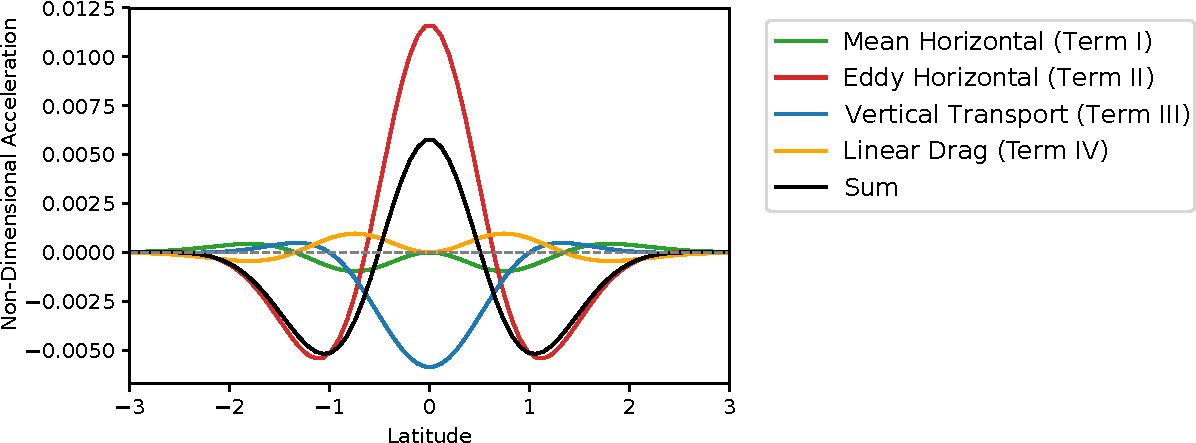
\includegraphics[width=1.0\textwidth]{figures/eqm-zonal-flow/beta-fluxes.pdf}
  \caption{Terms in the zonal-mean zonal momentum equation (Equation \ref{eqn:zonal-mean-mom}) with the correction $R$ to the momentum. The correction reduces the ``Vertical Transport'' term in Figure \ref{fig:beta-fluxes-no-R}, giving a net eastward acceleration at the equator.}
  \label{fig:beta-fluxes-with-R}
\end{figure}

Therefore, there is a positive acceleration on the equator unlike in Equation \ref{eqn:zonal-mean-mom-zeta-no-R}. Figure \ref{fig:beta-fluxes-with-R} shows the net positive acceleration at the equator due to the reduced ``Vertical Transport'' term (Term III in Equation \ref{eqn:zonal-mean-mom}). This explains the formation of eastward equatorial flow in the atmospheres of tidally locked planets. However, Figure \ref{fig:beta-fluxes-with-R} shows that this eastward equatorial flow requires westward flow at high latitudes, which is inconsistent with some GCM simulations. The next section will introduce the GRW mechanism to resolve this problem.



%
% %SUBSECTION -- SR and SBR
% \subsection{Super- and Sub-Rotation}\label{sec:super-sub-rotation}
%
% It is important to define the concept of ``superrotation'' precisely, to make the proposed effect of the meridional circulation clear. \citet{read2018superrotation} defines superrotation using the ``superrotation index'', which is a relative angular momentum excess compared to solid-body rotation at the equator \citep{read1986super}. The specific angular momentum $m$ is:
%
% \begin{equation}
%   m=a \cos \phi(\Omega a \cos \phi+u),
% \end{equation}
%
% and the local superrotation index is:
%
% \begin{equation}
%   s=\frac{m}{\Omega a^{2}}-1
% \end{equation}
%
% This provides a measure of the local momentum excess provided by momentum fluxes in the atmosphere -- generally, equatorward fluxes which produce a positive superrotation index. The global superrotation index is a mass-weighted integral of the local quantity:
%
% \begin{equation}
%   S_{m}=\frac{\iiint \rho m \mathrm{d} V}{\iiint \rho \Omega a^{2} \cos ^{2} \phi \mathrm{d} V}-1.
% \end{equation}
%
% \citet{read2018superrotation} highlights that $s$ and $S_{m}$ cannot exceed zero without up-gradient fluxes of angular momentum, a condition referred to as Hide's Theorem \citep{hide1969dynamics}. On a tidally locked planet, these are provided by the stationary horizontal eddy momentum fluxes discussed previously and shown in Figure \ref{fig:beta-fluxes-with-R}.
%
% The distinction between superrotating and subrotating flow, versus westerly and easterly flow, is vital to the conclusions of this chapter. The fluxes shown in Figure \ref{fig:beta-fluxes-with-R} operates on a background flow of zero. Therefore, any westerly flow at the equator requires easterly flow at high latitudes to conserve angular momentum. The GRW mechanism used in this chapter applies this system to a non-zero background flow, with a meridional circulation and westerly subtropical jet. Then, the equatorward momentum transport produces westerly superrotating flow at the equator -- but, it does not necessarily need to be compensated by easterly flow as before. Instead, it must be compensated by more subrotating flow (lower $s$) at higher latitudes. This subrotating flow can still be westerly, leading to the westerly flow at all latitudes seen in some GCM simulations.


%%%%%%%%%%%%%%%%%%%%%%%%%%%%
%SECTION 2 -- MERIDIONAL CIRCULATION
\section{Linear Model of the GRW Mechanism}

The meridional circulation of an atmosphere is driven by a difference in forcing between its equator and pole. On the Earth, it consists of multiple overturning cells that are approximately zonally uniform. The instellation on tidally locked planets is not zonally uniform so the meridional circulation should vary with longitude. Some studies have measured aspects of the meridional circulation of tidally locked planets in simulations of hot Jupiters and sub-Neptunes \citep{charnay20153d, showman2015circulation, mendoncca2018revisiting}. These studies did not consider the effect of the meridional circulation on the zonal flow, which I will discuss here.

The previous section showed that the linear shallow-water model of \citet{showman2010superrotation} explains the formation of equatorial superrotation, but requires westward flow at high latitudes to conserve angular momentum. This is not consistent with many GCM simulations that have eastward flow at all latitudes at the level of their equatorial jet \citep{kataria2015atmospheric,showman2015circulation,pierrehumbert2018review}. The shallow-water model is also not consistent with the evolution of angular momentum seen in GCM simulations. It predicts that the jet layer must lose angular momentum, as the only exchange of momentum out of the layer is a net loss to the lower layer via term III in Equation \ref{eqn:zonal-mean-mom}. Many simulations of tidally locked planets have positive net angular momentum at the level of their jet (and in total in their atmosphere) so contradict the linear model \citep{heng2015review, pierrehumbert2018review}.

Both of these problems could be resolved by a process that adds eastward acceleration to the jet layer at high latitudes. This section will suggest that the meridional circulation is this process, forming eastward subtropical jets via the ``Gierasch-Rossow-Williams'' mechanism that also produces the equatorial jet. I will demonstrate this mechanism in a linear and non-linear shallow-water models and an idealised GCM.


% This section will show how the predicted zonal flow in the linear shallow-water model of \citet{showman2011superrotation} can be inconsistent with GCM simulations. It will then introduce the GRW mechanism to resolve this problem, and modify the linear model to represent the effect of this mechanism. The following sections will demonstrate the mechanism in a non-linear shallow-water model and an idealised GCM.


% In this section, I will show that the linear shallow-water model of \citet{showman2011superrotation} is not consistent with some aspects of the zonal flow produced in GCM simulations of tidally locked planets. The shallow-water model requires easterly flow at high latitudes if there is to be westerly equatorial superrotation, but some GCM simulations have westerly flow at all latitudes at the level of their jet.

% I will introduce the Gierasch-Rossow-Williams (GRW) mechanism as a way to reconcile these differences. This mechanism combines the momentum transport of a meridional circulation with the equatorward momentum transport of the \citet{showman2011superrotation} mechanism (it was originally used to explain the superrotation of the atmosphere of Venus). I will show that the zonal mean meridional circulation can be considered to only depend on the zonal mean of the forcing, avoiding the difficult question of its longitudinal variation.
%
% The GRW mechanism then allows for westerly flow at all latitudes, as it pumps westerly momentum into the atmosphere from the surface and transports it to high latitudes. I will demonstrate this mechanism at work in a linear shallow-water model, a non-linear shallow-water model, and the GCM Exo-FMS. I will show that it requires subrotating (not superrotating) flow at high latitudes -- but this subrotating flow can still be westerly.


% %SUBSECTION -- PROBLEM WITH ACCELERATION AND MOMENTUM
% \subsection{Angular Momentum in the Shallow-Water Model}



%SUBSECTION -- PROPOSED MECHANISM
\subsection{The GRW Mechanism on a Tidally Locked Planet}\label{sec:grw-on-tl}

% In this section, I will introduce the GRW mechanism and show how it can be applied to a tidally locked planet. I will demonstrate that the zonal-mean meridional circulation -- a vital part of the mechanism -- can be approximated as only due to the zonal mean of the forcing, avoiding the complicated longitudinal variation of the meridional circulation.

The ``Gierasch-Rossow-Williams'' (GRW) mechanism was developed by \citet{gierasch1975meridional} and \citet{rossow1979large} to describe the formation of zonal flow in the atmosphere of Venus \citep{read2018superrotation}. Figure \ref{fig:gierasch} shows the GRW mechanism with the momentum fluxes particular to a tidally locked planet.
%
% In the mechanism, a mean meridional circulation has a westerly drag applied to the easterly flow in its lower branch. The westerly angular momentum added to the lower branch is then conveyed to the whole atmosphere by the meridional circulation. This circulation produces ``subtropical'' jets at high latitudes to conserve angular momentum as the upper branch travels towards the poles

The solid arrows in Figure \ref{fig:gierasch} show the momentum transport of the mean meridional circulation. I will explain later why this is treated as a zonal-mean process when it varies with longitude in reality. Hot air rises at the equator and travels towards the poles, accelerating eastward to conserve angular momentum. It falls at the poles, and then returns to the equator, accelerating westward to conserve momentum again. Drag from the surface applies a westerly torque to this lower branch, adding prograde eastward momentum to the entire atmosphere. The net effect of this mean meridional circulation is to produce eastward subtropical jets at high latitudes, and a total positive eastward atmospheric angular momentum. The ideal mechanism applies to a planet with a global Hadley cell, avoiding the multiple cells and jets seen on Earth.

The dashed lines in Figure \ref{fig:gierasch} show the momentum transport due to the wavenumber-1 ``eddy'' stationary wave response to day-night forcing \citep{showman2011superrotation}. The horizontal momentum flux in Figure \ref{fig:beta-fluxes-with-R} transports angular momentum towards the equator. This produces the eastward equatorial jet and applies a westward acceleration at high latitudes, which is opposed by the eastward acceleration at high latitudes due to the meridional circulation. I will show later that the horizontal and vertical transports balance at the equator in equilibrium, and the horizontal eddy transport balances the mean meridional transport at high latitudes.

This mechanism can resolve the problems introduced at the start of this section. The atmosphere and jet layer gain positive net angular momentum from the drag on the lower branch of the mean meridional circulation. The jet layer can have eastward flow at all latitudes, as the due to the westward acceleration at high latitudes in Figure \ref{fig:beta-fluxes-with-R} is opposed by the eastward acceleration from the meridional circulation. Instead of requiring westward flow at high latitudes to balance the eastward flow at the equator, this mechanism requires subrotating flow at high latitudes to balance the superrotating flow at the equator -- but, the subrotating flow can still be eastward.

\begin{figure}
  \centering
  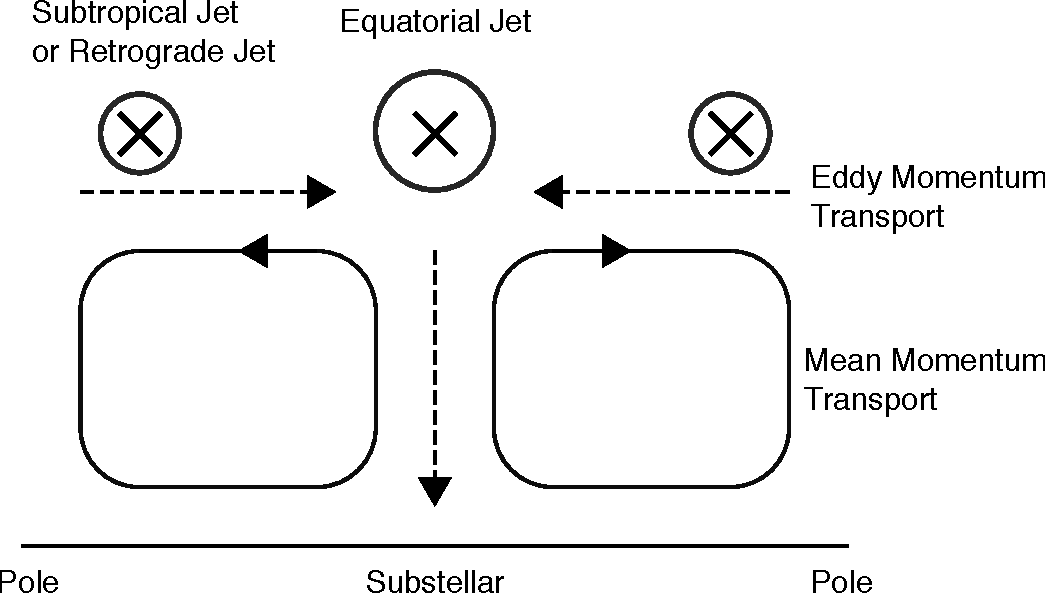
\includegraphics[width=0.75\textwidth]{figures/eqm-zonal-flow/gierasch-tl.pdf}
  \caption{The Gierasch-Rossow-Williams (GRW) mechanism \citep{read2018superrotation}, applied to the atmosphere of a tidally locked terrestrial planet. The solid line shows the mean momentum transport, which produces subtropical jets at high latitudes. The dashed lines show the horizontal and vertical momentum transports, which accelerate and decelerate the equatorial superrotation respectively.}
  \label{fig:gierasch}
\end{figure}


%%%%%%



% Figure \ref{fig:gierasch} shows the GRW mechanism \citep{read2018superrotation} as applied to the atmosphere of a tidally locked planet. The solid lines show the mean meridional circulation, which transports air up from the equator and poleward in the jet layer. It accelerates in this upper branch to conserve angular momentum as it travels poleward, creating westerly subtropical jets. The equatorward lower branch accelerates westward for the same reason and is dragged by the surface. This produces a net eastward torque on the atmosphere, which is conveyed to the upper layer by the meridional circulation. This results in a net positive angular momentum in both the jet layer and in the whole atmosphere.

% The dashed lines show the momentum transport terms due to the stationary wave response in a tidally locked planet \citep{showman2011superrotation}. These transport angular momentum equatorward in the jet layer, and downward at the equator. Later, I will show how they balance each other at the equator, and the transport from the mean meridional circulation at higher latitudes. This will explain how the number of zonal jets and their relative strength depends on the planetary parameters.

The idealised GRW mechanism in Figure \ref{fig:gierasch} assumes that the meridional circulation has the same zonal-mean effect on a tidally locked planet as on an asynchronously rotating planet like Venus. This ignores the longitudinal variation in this circulation due to the longitudinal variation in the equator-pole temperature gradient. In reality, the meridional circulation will be strongest at the substellar longitude, and negligible or even reversed on the night-side \citep{charnay20153d}. However, I will show that in the linear limit only the zonal mean of the meridional circulation is relevant to the momentum transport and jet formation discussed above.


%
% This provides an idealised picture of the momentum transports that produce the zonal flow on a tidally locked planet. However, it only applies to the zonal mean flow, and the zonal mean of the meridional circulation. In reality, the meridional circulation on a tidally locked planet will vary greatly with longitude. \citet{charnay20153d} suggests an ``anti-Hadley'' circulation of cells in the opposite direction to Hadley cells on the night-side of a tidally locked planet.
%
% This may make it difficult to apply the GRW mechanism in this case, as it relies on the zonal mean of the meridional circulation. However, I will show here that in the linear limit the meridional circulation on a tidally locked planet has a zonal mean that only depends on the zonal mean of the instellation -- so, the details of its longitudinal variation do not matter to the mechanism.
%
% LINEAR LIMIT INTRO
%
% Now, I will show that in the linear limit the meridional circulation is only governed by the zonal mean of the forcing (the zeroth-order term in Figure \ref{fig:decomp-forcing}).

\citet{held1980nonlinear} show that the properties of the meridional circulation 0-- zonal and meridional velocities, meridional momentum flux etc. -- are linear with response to the forcing. This holds separately at every longitude. The linearity of any property $X$ with respect to the forcing $Q(\phi,\lambda)$ means that for axisymmetric forcing, the zonal mean of $X$ has the property:

\begin{equation}
  \overline{X} \sim \overline{Q} =Q_{0}\cos{\phi}.
\end{equation}

For the same forcing on a tidally locked planet, the forcing is $ Q(\phi,\lambda)=Q_{0}\cos{\phi}\sin{\lambda}$ on the day-side, plus a uniform relaxation on the night-side. So, the zonal mean is:

\begin{equation}
  \overline{X} \sim \overline{Q} =Q_{0}\cos{\phi}\overline{\sin\lambda},
\end{equation}

where the mean of the $\sin \lambda$ is only taken over the day-side, giving:

\begin{equation}
  \overline{X} \sim Q_{0}\cos{\phi},
\end{equation}

The zonal mean of the meridional circulation therefore depends on the zonal mean of the forcing, when the local meridional circulation depends linearly on the local forcing. It is therefore possible to consider the zonal-mean effect of the meridional circulation on a tidally locked planet as entirely due to the wave-0 (zonal mean) component of the forcing. It is possible that non-linear effects from high forcing magnitudes or interactions with the zonal flow will make this assumption invalid.

% The accuracy of this approximation will be tested by how well it describes the results of GCM simulations later in this chapter.



%SUBSECTION -- LINEAR
\subsection{Demonstration in a Linear Shallow-Water Model}\label{sec:lin-sw-grw-results}

This section demonstrates the GRW mechanism on a tidally locked planet in a modified version of the linear shallow-water model of \citet{showman2011superrotation}. The model is modified by adding a zonally uniform meridional velocity $\overline{V}(y) = V_{0} \sin{y/y_{0}} e^{-y^{2}/y_{0}^{2}}$ to represent the poleward branches of the meridional circulation. The meridional scale is $y_{0}=\sqrt{2}$ as before and in \citet{matsuno1966quasi}, and the scale of the velocity is $V_{0} = 0.02$, chosen to produce an appropriate acceleration magnitude for this demonstration.


% Figure \ref{fig:beta-fluxes-plus-merid} shows the zonal-mean zonal acceleration in this linear model, when a zonally uniform background meridional velocity $\overline{V}(y) = V_{0} \sin{y/y_{0}} e^{-y^{2}/2}$ is imposed.



\begin{figure}
  \centering
  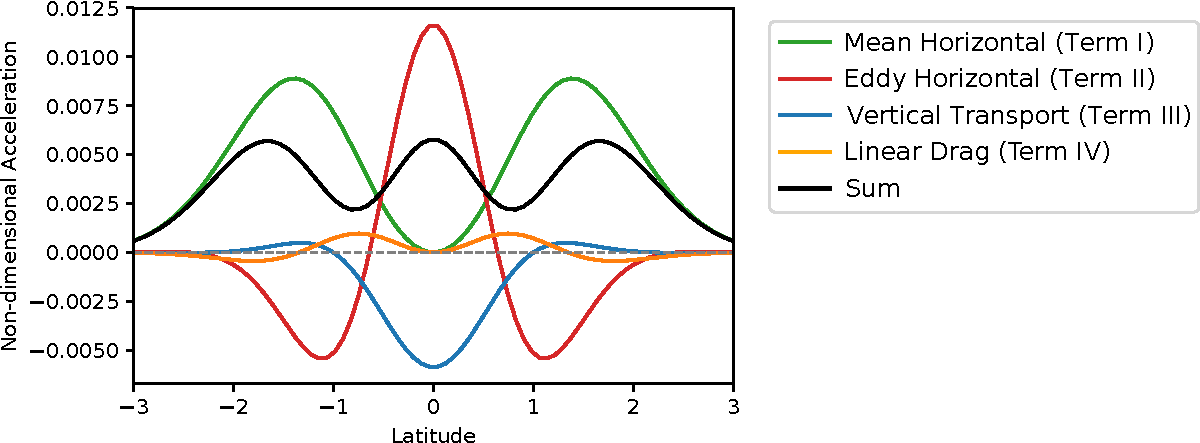
\includegraphics[width=1.0\textwidth]{figures/eqm-zonal-flow/beta-fluxes-plus-merid.pdf}
  \caption{Acceleration terms in the zonal-mean zonal momentum equation (Equation \ref{eqn:zonal-mean-mom}), with an imposed uniform zonal-mean meridional velocity $\overline{V}(y) = V_{0} \sin{y/y_{0}} e^{-y^{2}/y_{0}^{2}}$, showing prograde westerly acceleration at all latitudes.}
  \label{fig:beta-fluxes-plus-merid}
\end{figure}

% Figure \ref{fig:beta-fluxes-with-R} showed how the linear shallow-water model in \citet{showman2011superrotation} predicts equatorial superrotation, but requires easterly acceleration at high latitudes. In this chapter, I have intoduced the idea that a meridional circulation can produce westerly acceleration at high latitudes, resulting in westerly flow at all latitudes. This can be demonstrated simply in a modified version of the linear shallow-water model.

The imposed meridional velocity affects Term I in Equation \ref{eqn:zonal-mean-mom}, producing a westerly acceleration at high latitudes around the peak of the imposed meridional flow $\overline{V}(y)$. This opposes the easterly acceleration due to horizontal momentum transport from stationary eddies in the previous linear model, producing westerly prograde acceleration at all latitudes if the meridional velocity is large enough. In the GRW mechanism, this reflects the fact that the equatorward momentum transport from stationary eddies is moving momentum from a region that is already accelerated eastward by the meridional circulation.

So, rather than requiring easterly flow above a certain latitude as in the linear model of \citet{showman2011superrotation}, this model requires sub-rotating flow above a certain latitude -- but, the flow can still be eastward. Next, I will use a non-linear shallow-water model and a GCM to demonstrate the mechanism without needing to impose the meridional circulation, as it will emerge naturally from the forcing in the models.

 % An additional problem is that the forcing in the idealised linear shallow-water model of \citet{showman2011superrotation} has zero zonal mean, which suggests that there is no meridional circulation at all.



%%%%%%%%%%%%%%%%%%%%%%%%%%%%
%SECTION 3 -- NONLINEAR MODEL
\section{Non-Linear Model of the GRW Mechanism}\label{sec:nonlin-shallow}

This section demonstrates the GRW mechanism in a non-linear time-stepped shallow-water model. The meridional circulation and the acceleration at high latitudes will emerge naturally from the forcing field, unlike in the linear model where the meridional velocity was imposed. I will show that the equilibrium zonal flow is governed by the balance of momentum fluxes predicted by the GRW mechanism.



%%%%%%


 %I will show the effect of the realistic radiative-equilbrium forcing field introduced earlier, and the effects of its wave-0 and wave-1 forcing components.

  % The balance of momentum fluxes for steady-state zonal flow is the same in this non-linear model as in the GCM and in the linear shallow-water model, suggesting that the GRW mechanism is a robust description of the formation of this zonal flow.

%SUBSECTION --
\subsection{Non-Linear Shallow-Water Model}

The GFDL Spectral Dynamical Core\footnote{\url{gfdl.noaa.gov/idealized-spectral-models-quickstart/}} solves the equations describing the fluid dynamics of a model atmosphere by representing the solution as a series of spherical harmonic functions \citep{polvani2004numerically}. In this section, it is configured to solve the non-linear shallow-water equations in a single layer \citep{showman2011superrotation}. The non-linear shallow-water equations in this model\footnote{\url{gfdl.noaa.gov/wp-content/uploads/files/user_files/pjp/shallow.pdf}} retain the terms that are discarded by the linear shallow-water equations in the previous section. The model is forced by relaxation to a radiative equilibrium height field $h_{eq}$, where a tendency $\Delta h$ is applied to the height field $h$ at every timestep:

\begin{equation}
  \Delta h = \Delta t (h - h_{eq}) / \tau_{rad} ,
\end{equation}

where $\Delta t$ is the timestep and $\tau_{rad}$ is the thermal damping timescale. The only other forcing is the correction $R$ to the zonal momentum \citep{shell2004superrotation}. The model could apply dynamical damping to the velocity fields of the shallow-water layer, but I chose not to use this damping in order to match the GCM simulations better. Section \ref{sec:gcm-sim-grw} will show that dynamical damping is not part of the balance of forces on the jet in the GCM.

I ran three simulations in the model which were forced by relaxation to different radiative equilibrium height fields $h_{eq}$. The models were run for 100 days, and the results taken over the last 10 days after a steady state had formed.  All the tests in this section have $h_{0} = \SI{10}{\kilo\metre}$, $\Delta h = \SI{1}{\kilo\metre}$, and a thermal damping time $\tau_{rad}=$ 0.1 days. Figures \ref{fig:nonlin-test-A}, \ref{fig:nonlin-test-B}, and \ref{fig:nonlin-test-C} show the height fields and zonal-mean zonal and meridional velocities of each test.




% he non-zero wave-0 component shows that there is a non-zero zonal-mean forcing on the atmosphere which will produce a mean meridional circulation. The wave-1 component is the forcing considered by \citet{showman2011superrotation}, which produces the equatorial superrotation.

%TODO: WAVE 1 AND 0 COMPONENTS HAVE SIMILAR OR SAME MAGNITUDE



%SUBSECTION --
\subsection{Test A: Sinusoidal Forcing}



\begin{figure}
  \centering
  \begin{subfigure}[t]{0.52\textwidth}
    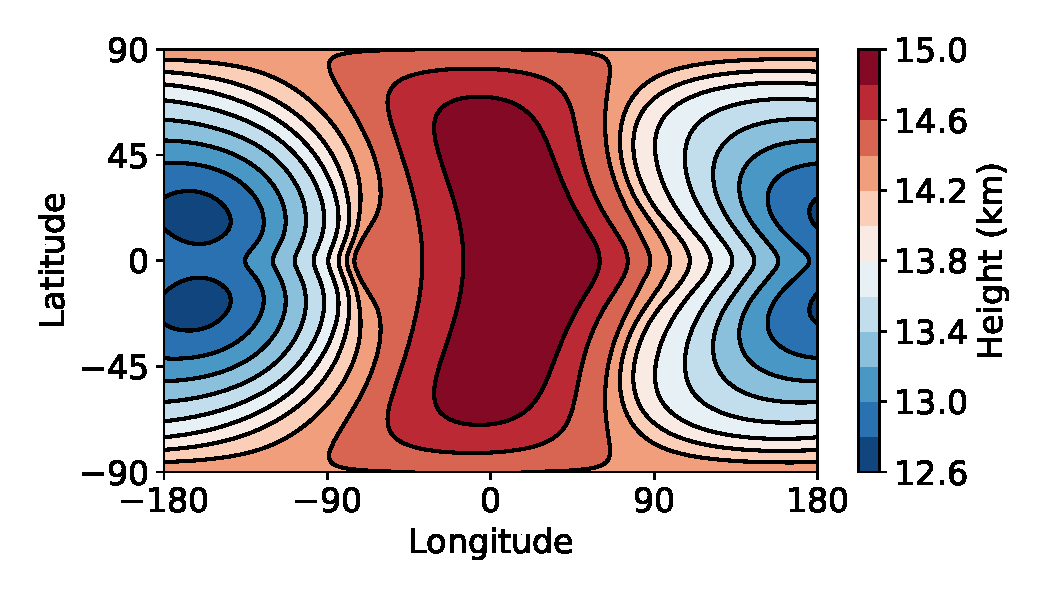
\includegraphics[width=1.0\textwidth]{figures/eqm-zonal-flow/test-A-h.pdf}
    \caption{Equilibrium height field.}
    \label{fig:test-A-h}
  \end{subfigure}
  %
  \begin{subfigure}[t]{0.47\textwidth}
    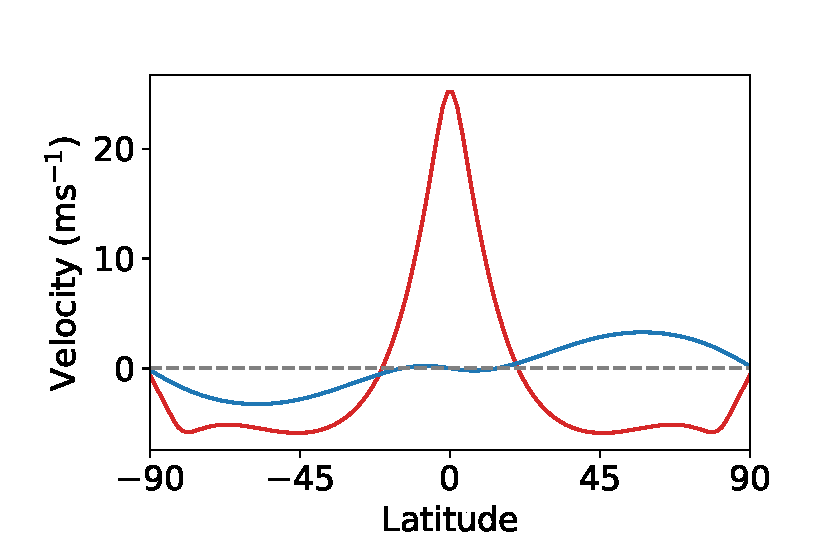
\includegraphics[width=1.0\textwidth]{figures/eqm-zonal-flow/test-A-u-v.pdf}
    \caption{$\overline{U}(y)$ (red) and $\overline{V}(y)$ (blue).}
    \label{fig:test-A-u-v}
  \end{subfigure}
  \caption{Test A with sinusoidal day-night forcing, showing the equilibrium height field, the zonal-mean zonal velocity $\overline{U}(y)$ (red), and the zonal-mean meridional velocity $\overline{V}(y)$ (blue). The height field shows the stationary wave response that produces an eastward equatorial jet and westward flow at high latitudes.}
  \label{fig:nonlin-test-A}

  \centering
  \begin{subfigure}[t]{0.52\textwidth}
    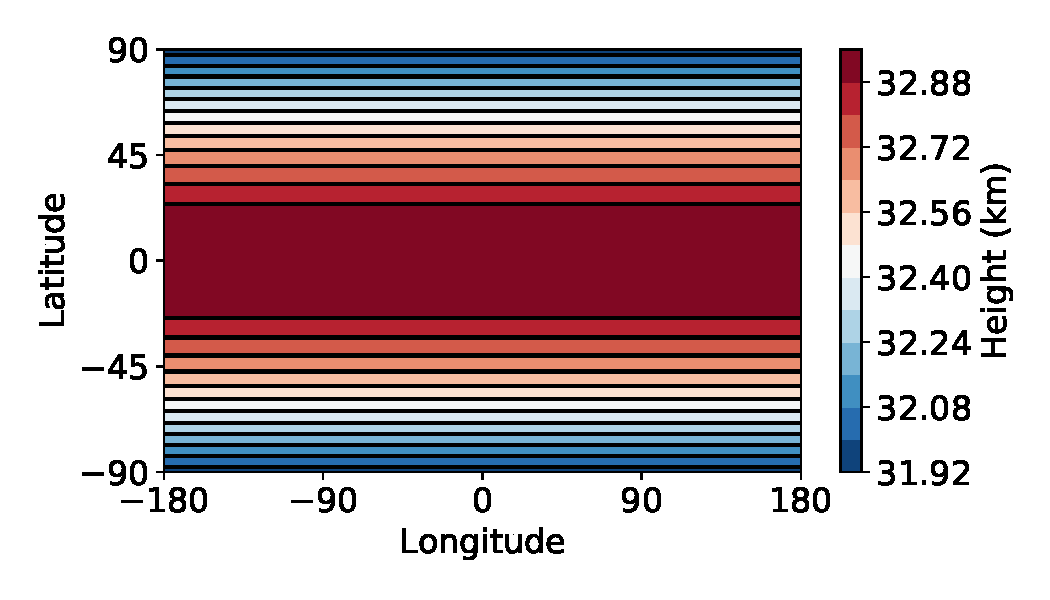
\includegraphics[width=1.0\textwidth]{figures/eqm-zonal-flow/test-B-h.pdf}
    \caption{Equilibrium height field.}
    \label{fig:test-B-h}
  \end{subfigure}
  %
  \begin{subfigure}[t]{0.47\textwidth}
    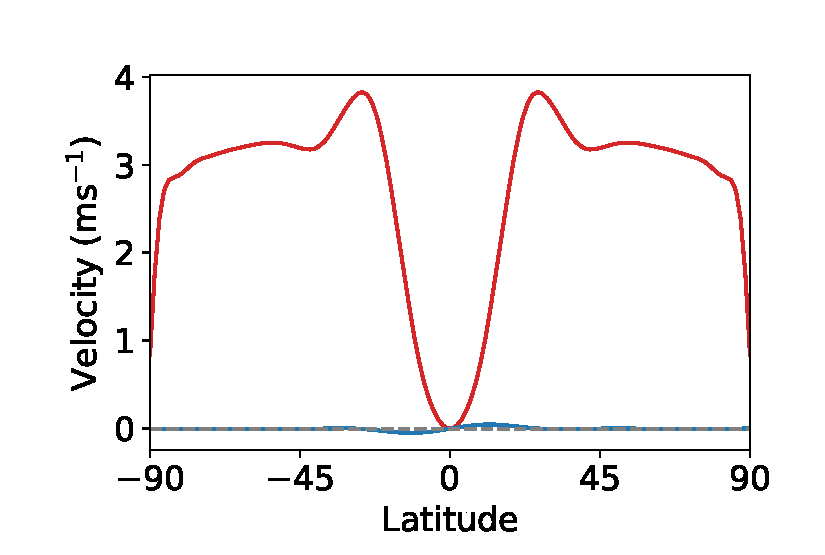
\includegraphics[width=1.0\textwidth]{figures/eqm-zonal-flow/test-B-u-v.pdf}
    \caption{$\overline{U}(y)$ (red) and $\overline{V}(y)$ (blue).}
    \label{fig:test-B-u-v}
  \end{subfigure}
  \caption{Test B with axisymmetric forcing, showing the axisymmetric height field and the meridional velocity that produces eastward subtropical jets.}
  \label{fig:nonlin-test-B}

  \centering
  \begin{subfigure}[t]{0.52\textwidth}
    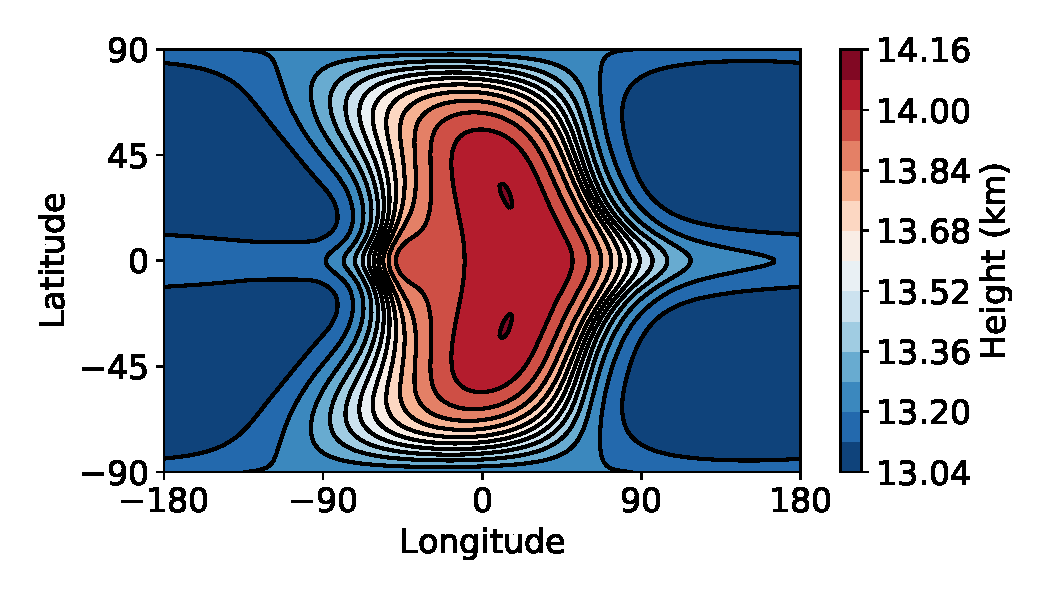
\includegraphics[width=1.0\textwidth]{figures/eqm-zonal-flow/test-C-h.pdf}
    \caption{Equilibrium height field.}
    \label{fig:test-C-h}
  \end{subfigure}
  %
  \begin{subfigure}[t]{0.47\textwidth}
    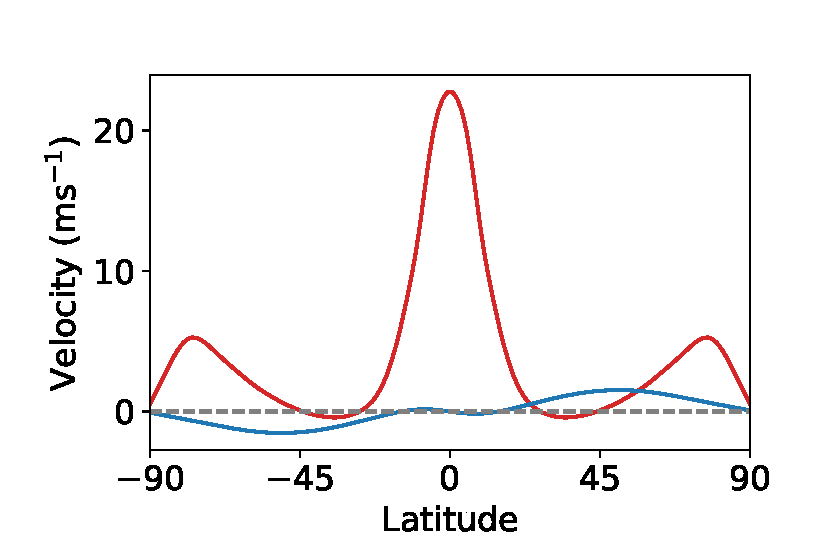
\includegraphics[width=1.0\textwidth]{figures/eqm-zonal-flow/test-C-u-v.pdf}
    \caption{$\overline{U}(y)$ (red) and $\overline{V}(y)$ (blue).}
    \label{fig:test-C-u-v}
  \end{subfigure}
  \caption{Test C with realistic forcing, showing the stationary wave response and the meridional velocity, which together produce eastward flow at all latitudes by the GRW mechanism.}
  \label{fig:nonlin-test-C}
\end{figure}


Test A was forced by relaxation to a radiative-equilibrium height field that varies sinusoidally with longitude:

\begin{equation}
  h_{eq} = h_{0} + \Delta h \sin \lambda \cos\phi.
\end{equation}

This is the same as the forcing field used in the linear model of \citet{matsuno1966quasi} and the non-linear model of \citet{showman2011superrotation}. It is a simple representation of day-side heating and night-side cooling, but does not produce a mean meridional circulation as it has zero zonal mean.

Figure \ref{fig:test-A-h} shows the resulting height field in equilibrium, which is similar to the non-linear simulations in Figure 8 of \citet{showman2011superrotation}. The model is forced in the same way as the linear response in Figure \ref{fig:beta-plane-forced}, but the non-linearity produces a day-night asymmetry in this case. The stationary waves created by the forcing transport eastward momentum towards the equator, producing an eastward equatorial jet and westward flow at high latitudes shown in Figure \ref{fig:test-A-u-v}. Note that there is some meridional velocity due to the small day-night asymmetry from the non-linear terms, but it is not strong enough to produce eastward subtropical jets. The stationary waves are partly shifted eastwards by this zonal-mean zonal velocity. As shown in Section \ref{sec:lin-sw-model}, the sinusoidal forcing must produce westward flow at high latitudes to balance the eastward flow at the equator, so is inconsistent with GCM simulations that can have eastward flow at all latitudes at the level of the jet \citep{showman2015circulation,kataria2015atmospheric,pierrehumbert2018review}.


%SUBSECTION --
\subsection{Test B: Axisymmetric Forcing}

The GRW mechanism requires a meridional circulation that produces eastward flow at the level of the jet at high latitudes. \citet{shell2004superrotation} model the meridional circulation of the Earth in a non-linear shallow-water model with an axisymmetric forcing with an equator-pole gradient. This produces a meridional velocity and eastward subtropical jets. The single-layer model does not represent the lower branch of the circulation, which would produce westward zonal flow. This will be represented in the GCM simulations later, where the westward surface flow will be a source of eastward atmosphere angular momentum due to Rayleigh drag.

Test B uses a simplified axisymmetric field to qualitatively reproduce the Earth-like circulation in \citet{shell2004superrotation}, and to show that a forcing field with a non-zero zonal mean produces an acceleration at high latitudes. The axisymmetric field is:

\begin{equation}
  h_{eq} = h_{0} + \Delta h \cos\phi / \pi.
\end{equation}

Figure \ref{fig:test-B-h} shows the axisymmetric height field in equilibrium, with a small equator-pole height gradient due to the forcing. The height gradient produces the meridional velocity shown in Figure \ref{fig:test-B-u-v}, that results in eastward zonal subtropical jets. Note that there is zero zonal flow at the equator. The next test will show how these subtropical jets are modified by equatorward momentum transport from the stationary wave forcing in Test A.


%%%

% This is equivalent to the wave-0 component of the ``realistic'' radiative-equilibrium field in Section \ref{sec:grw-on-tl}. It produces the same type of meridional circulation as the non-linear model in \citet{shell2004superrotation}. This Hadley circulation adds momentum to the layer represented by the shallow-water model, producing westerly zonal flow at high latitudes to conserve angular momentum. In a real atmosphere, momentum would be conserved by the formation of easterly flow in the lower branch of the circulation (although as shown earlier, this is dragged by the surface, resulting in net positive westerly momentum after all).

%SUBSECTION --
\subsection{Test C: Realistic Forcing}

Test C uses a more realistic forcing field to show how the GRW mechanism can produce eastward flow at all latitudes. The forcing field in Test A is not realistic because the night-side should cool uniformly, rather than preferentially at the antistellar point. A more realistic radiative-equilibrium field is:

\begin{equation}
  h_{eq}=\begin{cases}
  h_{0} + \Delta h \sin \lambda \cos\phi & ( |\lambda | < \pi / 2 ) \\
  h_{0} & ( |\lambda | > \pi / 2 )
\end{cases}
\end{equation}


\citet{perez2013atmospheric} used a similar height field in a model of a tidally locked planetary atmosphere. Unlike the field in Test A, the field in Test C has a non-zero zonal mean. The zonal mean of this forcing is the same as the axisymmetric forcing in Test B, so it should produce a similar meridional circulation. The day-side component of this realistic field is the same as the day-side of Test A, so it should give similar stationary waves and equatorward momentum transport. Together, these components drive the GRW mechanism -- the zonal-mean forcing field produces eastward zonal flow at high latitudes, then the stationary waves transport eastward momentum towards the equator. The forcing fields of Tests A and B are essentially the lowest-order Fourier components of Test C, where Test B is the zeroth-order component and Test A is the first-order component.

Figure \ref{fig:test-C-h} shows the equilibrium height field of Test C, which is similar to the height field of Test A. The stationary waves are weaker on the night-side than the day-side, which may be due to the uniform forcing on the night-side. Figure \ref{fig:test-C-u-v} shows the key result of this section -- eastward zonal flow at all latitudes, as predicted by the GRW mechanism. This is a result of the meridional circulation producing acceleration at high latitudes, which is too strong to be reversed by the equatorward momentum transport that creates the equatorial jet.

The GRW mechanism modifies the requirement of \citet{showman2011superrotation} of westward flow at high latitudes to a requirement of subrotating flow at high latitudes (see \ref{sec:superrotation} for the definition of subrotation). The next section will investigate the balance of sources of acceleration at different latitudes in Test C.




%
% \begin{figure}
%   \centering
%   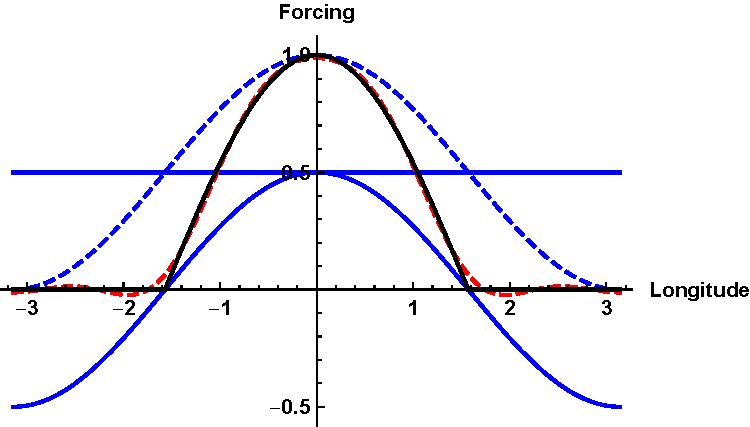
\includegraphics[width=0.7\textwidth]{figures/eqm-zonal-flow/fourier.pdf}
%   \caption{The Fourier series of the realistic forcing.}
%   \label{fig:decomp-forcing}
% \end{figure}



%
%
% The black line in Figure \ref{fig:decomp-forcing} shows the longitudinal form of this radiative equilibrium field on the equator. The red dashed line shows an approximation by a fifth-order Fourier series. The blue dashed line shows the sum of the wave-0 and wave-1 Fourier components (the solid blue lines), which approximates the real field and crucially has a non-zero zonal mean. The first-order term corresponds to the radiative equilibrium field in \citet{showman2011superrotation} -- adding the zeroth-order term adds a non-zero zonal mean.


\subsection{Equilibrium Zonal Flow}

The mechanism in Figure \ref{fig:gierasch} predicts the balance of momentum fluxes that determine the equilibrium state of the zonal flow. At the equator, the horizontal momentum transport from the stationary waves should balance the vertical momentum transport from rising and subsiding air at the substellar and antistellar points. At high latitudes, the horizontal momentum transport from the stationary waves should be balanced by the eastward acceleration of the poleward branch of the meridional circulation. This section will test this prediction in the non-linear shallow-water model.

The zonal-mean momentum equation in a spherical geometry is \citep{showman2011superrotation}:

\begin{equation}\label{eqn:zonal-mean-mom-sphere}
  \begin{split}
    \frac{\partial \overline{u}}{\partial t}=\underbrace{\overline{v}^{*}\left[f-\frac{1}{a \cos \phi} \frac{\partial(\overline{u} \cos \phi)}{\partial \phi}\right]}_{\mathrm{I}}
    \underbrace{-\frac{1}{\overline{h} a \cos ^{2} \phi} \frac{\partial}{\partial \phi}\left[\overline{(h v)^{\prime} u^{\prime}} \cos ^{2} \phi\right]}_{\mathrm{II}} \\
    +\underbrace{\left[\frac{1}{\overline{h}} \overline{u^{\prime} Q^{\prime}}+\overline{R_{u}}^{*}\right]}_{\text { III }} \underbrace{-\frac{\overline{u}^{*}}{\tau_{\mathrm{drag}}}}_{\mathrm{IV}}-\frac{1}{\overline{h}} \frac{\partial\left(\overline{h^{\prime} u^{\prime}}\right)}{\partial t},
  \end{split}
\end{equation}


where $\phi$ is longitude, and all other variables are the same as before. Figure \ref{fig:test-C-accn} shows each of these terms for the steady-state flow in Test C. The ``Mean horizontal'' term is Term I, which produces an acceleration at high latitudes due to the mean meridional velocity. This is primarily balanced by the ``Eddy Horizontal'' flux of Term II, which produces a westward acceleration at high latitudes as it transports eastward momentum towards the equator. This is the balance predicted by Figure \ref{fig:gierasch} and shown in the linear model in Section \ref{sec:lin-sw-grw-results}. There is also a westward acceleration at high latitudes from the ``Vertical Transport'' flux of Term III, as the eastward flow subsides in the descending branch of the meridional circulation. At the equator, the balance is between eastward acceleration due to the ``Eddy Horizontal'' transport from the stationary waves, and westward acceleration due to the ``Vertical Transport'' term discussed in Section \ref{sec:lin-sw-model}. Term I is zero at the equator as there is zero meridional velocity. This agrees with the mechanism in Figure \ref{fig:gierasch} and Section \ref{sec:lin-sw-grw-results}.

\begin{figure}
  \centering
  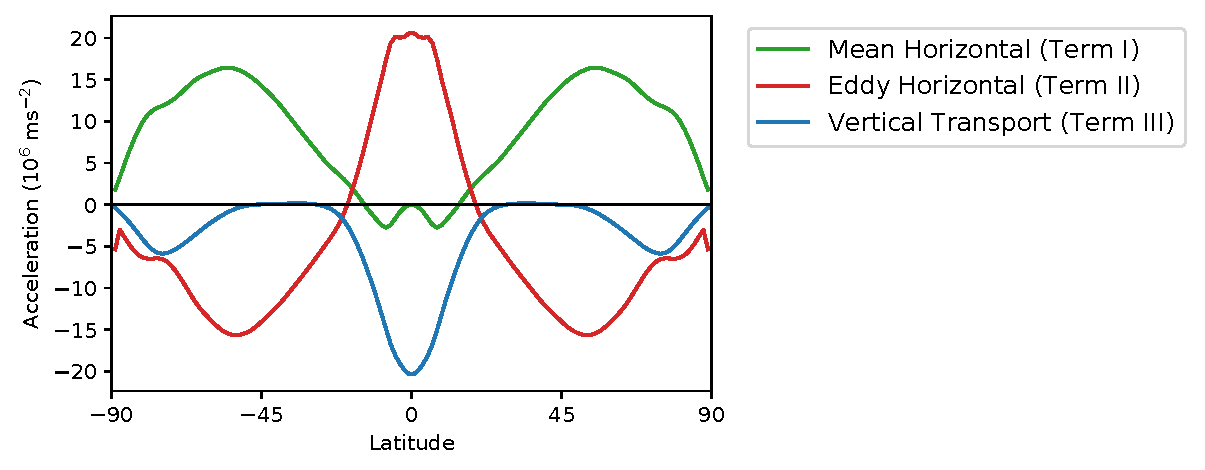
\includegraphics[width=1.0\textwidth]{figures/eqm-zonal-flow/nonlin-balance.pdf}
  \caption{The terms in the zonal-mean zonal momentum equation (Equation \ref{eqn:zonal-mean-mom-sphere}) for Test C with realistic forcing in the non-linear shallow-water model, showing how equilibrium is achieved at the equator and at high latitudes. Note the same balance of forces as in Figures \ref{fig:beta-fluxes-plus-merid} and \ref{fig:accn-terms-jet-level}.}\label{fig:test-C-accn}
\end{figure}


These non-linear shallow-water simulations have shown how the sinusoidal day-night forcing produces an equatorward momentum transport, how a non-zero zonal-mean forcing produces a meridional circulation, and how a realistic forcing combines these processes to drive the GRW mechanism. The realistic forcing field in Test C produces eastward flow at all latitudes, matching the GCM simulations that could not be explained by the model with sinusoidal day-night forcing. The balance of momentum fluxes at the equator and at high latitudes matched the balance predicted by the GRW mechanism. In the next section, I will show this is also the case in idealised GCM simulations of the atmosphere of a tidally locked planet.


% At the equator, the horizontal stationary momentum flux (Term II) balances the vertical stationary momentum flux (Term III). At high latitudes, the horizontal mean momentum flux (Term I) balances the horizontal stationary momentum flux (Term II).


%
% In the next section, I will apply  the GRW mechanism to predict scaling relations for the zonal flow in the non-linear shallow-water model and the GCM.





% \begin{figure}
%   \centering
%   \begin{subfigure}[t]{0.32\textwidth}
%     \includegraphics[width=1.0\textwidth]{figures/eqm-zonal-flow/test-1-accn.pdf}
%     \caption{1}
%     \label{fig:test-1-accn}
%   \end{subfigure}
%   %
%   \begin{subfigure}[t]{0.32\textwidth}
%     \includegraphics[width=1.0\textwidth]{figures/eqm-zonal-flow/test-2-accn.pdf}
%     \caption{2}
%     \label{fig:test-2-accn}
%   \end{subfigure}
%   %
%   \begin{subfigure}[t]{0.32\textwidth}
%     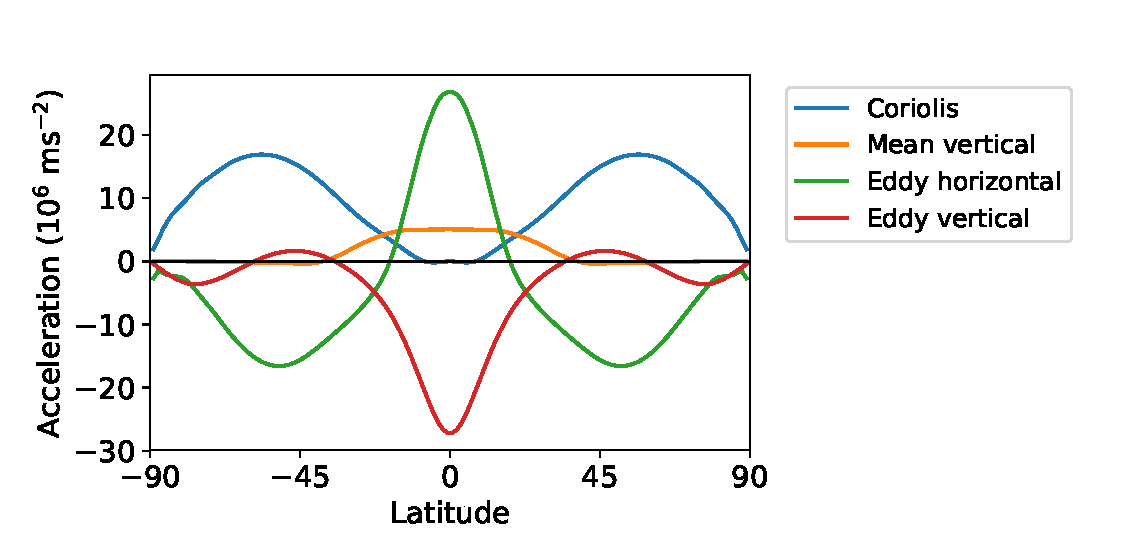
\includegraphics[width=1.0\textwidth]{figures/eqm-zonal-flow/test-3-accn.pdf}
%     \caption{3}
%     \label{fig:test-3-accn}
%   \end{subfigure}
%   \caption{Accelerations.}
%   \label{fig:nonlin-tests-accn}
% \end{figure}


%SECTION CONCLUSIONS

\section{GCM Simulations of the GRW Mechanism}\label{sec:gcm-sim-grw}

This section shows the formation of zonal flow in the GCM Exo-FMS. I will compare an idealised simulation of a tidally locked planet to a simulation of an asynchronously rotating planet, and show that the balance of momentum fluxes in the GCM is same as the shallow-water models in the previous section. The next section will use this mechanism to predict the scaling behaviour of the zonal flow in a suite of tests in the non-linear shallow-water model and the GCM.

Test 1 is a tidally locked planet with a pure $N_{2}$ atmosphere with radius  $1.0\ R_{E}$, rotation rate $\Omega_{E}/10$, surface pressure $\SI{1}{\bar}$, longwave optical thickness $1.0$, shortwave optical thickness $0.0$, and instellation $\SI{1000}{\watt\per\metre\squared}$. This test is an idealised, general example of a tidally locked terrestrial planet orbiting an M-dwarf, using Exo-FMS with semi-grey radiative transfer and dry convective adjustment.

Figure \ref{fig:default-gcm-temp} shows the equilibrium global circulation of Test 1, time-averaged from 1000 to 2000 days of the simulation. The global temperature and wind fields show the typical superrotating jet and hot-spot shift seen on tidally locked planets \citep{showman2012review, pierrehumbert2018review}. The zonal-mean zonal wind is dominated by a single equatorial jet, which is shown in Chapter \ref{ch:wave-mean-flow} to produce the hot-spot shift by shifting the stationary planetary waves eastward. Note that there is prograde eastward flow at all latitudes of the jet in this test, which is the situation that this chapter aims to explain.

Test 2 is an asynchronously rotating planet with otherwise the same properties as Test 1. Its instellation is zonally uniform but has the same zonal-mean instellation as Test 1. I will show that this produces the same meridional circulation on the first day of the test when the response to forcing is small and linear. Figure \ref{fig:default-gcm-axi-example} shows the global circulation of the equilibrium state of Test 2, time-averaged from 1000 to 2000 days of the simulation. This atmosphere has an zonally uniform temperature field, and two subtropical jets produced by its meridional circulation. Its ``Hadley'' cells are global due to its 10 day rotation period, unlike the more rapidly rotating Earth with its multiple cells.

 These two tests will show how the meridional circulation on a tidally locked planet produces subtropical jets before the stationary waves from the day-night forcing produce equatorial acceleration, as described by the GRW mechanism. \citet{norton2006tropical} used similar simulations to these two tests to show the formation of superrotation by tropical heating on the Earth.

\begin{figure}
  \centering
  \begin{subfigure}[t]{0.48\textwidth}
    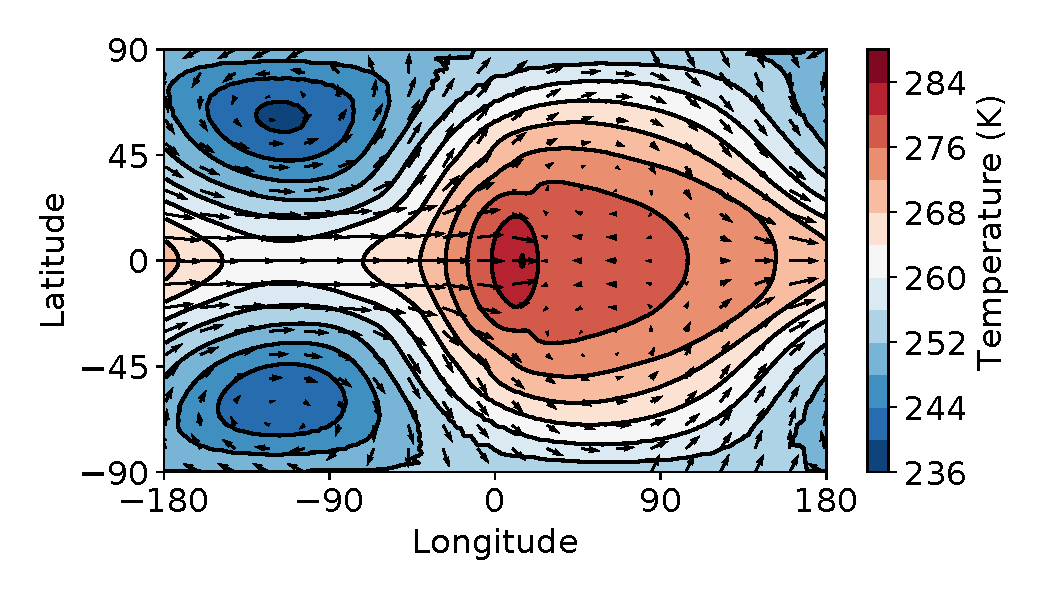
\includegraphics[width=1.0\textwidth]{figures/eqm-zonal-flow/default-gcm-temp.pdf}
    \caption{Temperature and velocity fields.}\label{fig:default-gcm-temp}
  \end{subfigure}
\quad
  \begin{subfigure}[t]{0.48\textwidth}
    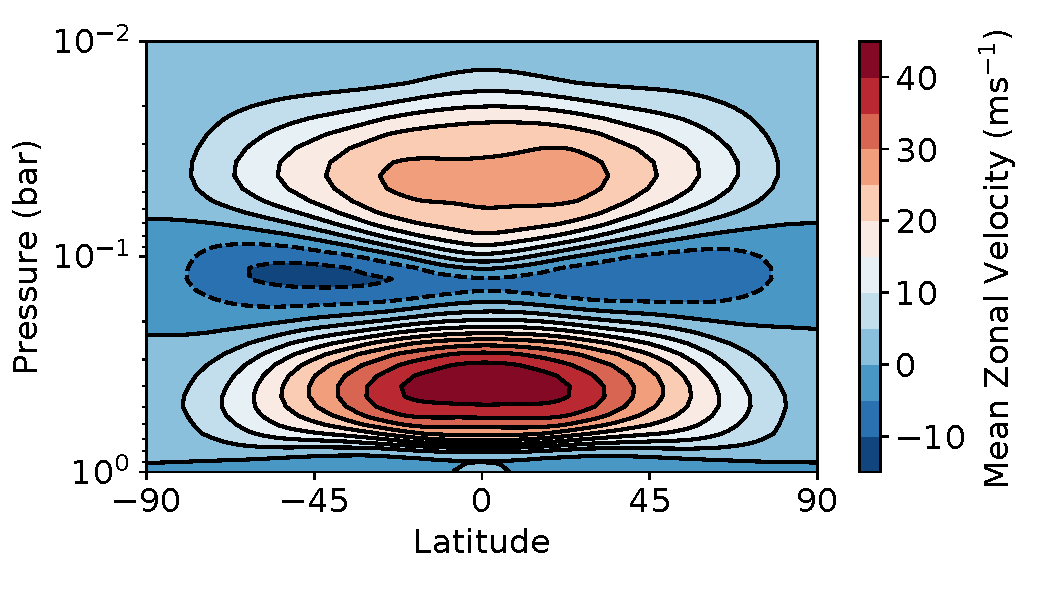
\includegraphics[width=1.0\textwidth]{figures/eqm-zonal-flow/default-gcm-zonal-flow.pdf}
    \caption{Zonal-mean zonal velocity.}\label{default-gcm-zonal-flow}
  \end{subfigure}
  \caption{The global circulation of Test 1, time-averaged from 1000 to 2000 days of the simulation. The temperature field is at the half-surface pressure level. This is a typical tidally locked Earth-sized planet, with prograde zonal flow at all latitudes at the level of maximum jet flow.}\label{fig:default-gcm-example}
\end{figure}


\begin{figure}
  \centering
  \begin{subfigure}[t]{0.48\textwidth}
    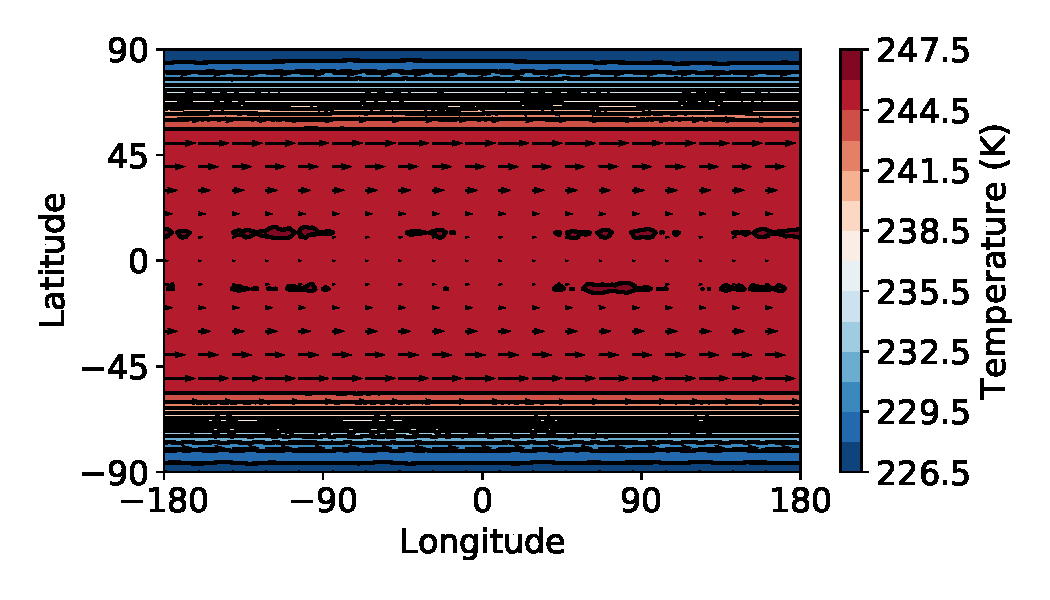
\includegraphics[width=1.0\textwidth]{figures/eqm-zonal-flow/default-gcm-axi-temp.pdf}
    \caption{Temperature and velocity fields.}\label{fig:default-gcm-axi-temp}
  \end{subfigure}
\quad
  \begin{subfigure}[t]{0.48\textwidth}
    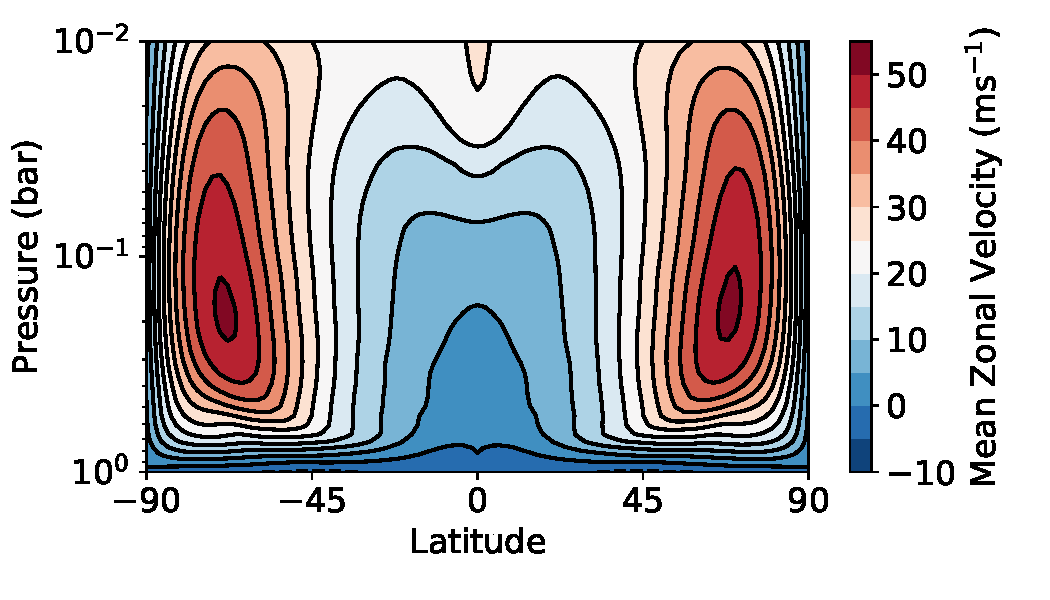
\includegraphics[width=1.0\textwidth]{figures/eqm-zonal-flow/default-gcm-axi-zonal-flow.pdf}
    \caption{Zonal-mean zonal velocity.}\label{default-gcm-axi-zonal-flow}
  \end{subfigure}
  \caption{The global circulation of Test 2, time-averaged from 1000 to 2000 days of the simulation. The temperature field is at the half-surface pressure level. This is an idealised asynchronously rotating Earth-sized planet, with subtropical jets formed by the mean meridional circulation.}\label{fig:default-gcm-axi-example}
\end{figure}


\subsection{Initial Meridional Circulation}

Section \ref{sec:grw-on-tl} suggested that the meridional circulation on a tidally locked planet primarily depends on the zonal mean of the instellation. This means that the longitudinal variation of the instellation and circulation does not greatly affect the GRW mechanism. Figure \ref{fig:day-1-tide-axi} shows that this is true for the early stages of Tests 1 and 2, when the response to forcing is small and linear. The first column shows the zonal velocity in the first day at the surface of each test, where Test 1 has diverging flow from the substellar point and Test 2 has weak surface westerlies forming as part of a meridional circulation.

The second column shows the zonal-mean zonal velocity on the first day. The two tests have almost exactly the same zonal-mean zonal velocity, despite their different longitudinal variation. The third column shows that they also have almost the same streamfunction. This supports the argument in Section \ref{sec:grw-on-tl} that only the zonal mean of the forcing (the same in Tests 1 and 2) affects the zonal-mean meridional circulation in the linear limit of weak forcing. The meridional circulation only enters the zonal-mean zonal momentum equation \citep{showman2011superrotation} as a zonal-mean quantity, so the GRW mechanism can be applied to the zonal-mean circulation without considering the actual longitudinal variation of the instellation. In reality, as each test spins up the assumption of linearity will become less accurate as the perturbations increase and the zonal flow affects the meridional circulation.

These tests support the use of the GRW mechanism to explain the formation of zonal flow on tidally locked planets. They show that the meridional circulation primarily affects the zonal flow through its zonal mean only. The next section will show how the equatorward momentum transport on tidally locked planets modifies the subtropical jets and produces equatorial superrotation.



%
% It shows the time-mean results of the first day of spin-up of these simulations from rest, where the response to the applied forcing is still small and linear. The leftmost panels show the highly different zonal winds at the surface of the tidally locked Test 1, and the surface of the axisymmetric Test 2. However, the next panels are the zonal mean zonal-wind of each test, showing the identical subtropical jets beginning to be formed by the mean meridional circulation in each case. These are the same due to the linearity demonstrated above -- the mean meridional circulation only depends on the zonal mean of the forcing, which is the same in Tests 1 and 2. The final panels show the same effect -- each test has the same zonal-mean mass streamfunction, as the meridional circulation is the same.
%
% This means that the effect of the mean meridional circulation on the zonal mean momentum equation (through term I in Equation \ref{eqn:zonal-mean-mom}) is the same in the tidally locked Test 1 as in the axisymmetric Test 2.


\begin{figure}
  \centering

  \begin{subfigure}[t]{0.31\textwidth}
    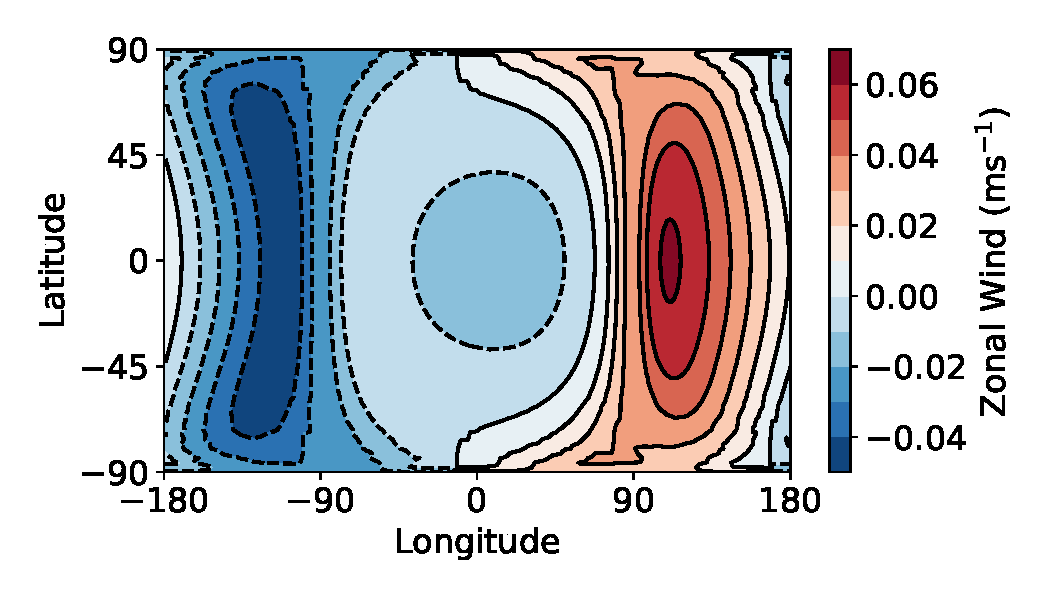
\includegraphics[width=\textwidth]{figures/eqm-zonal-flow/zonal-wind-map-tide-day1.pdf}
    \caption{1: Surface zonal velocity.}
  \end{subfigure}
\enskip
  \begin{subfigure}[t]{0.31\textwidth}
    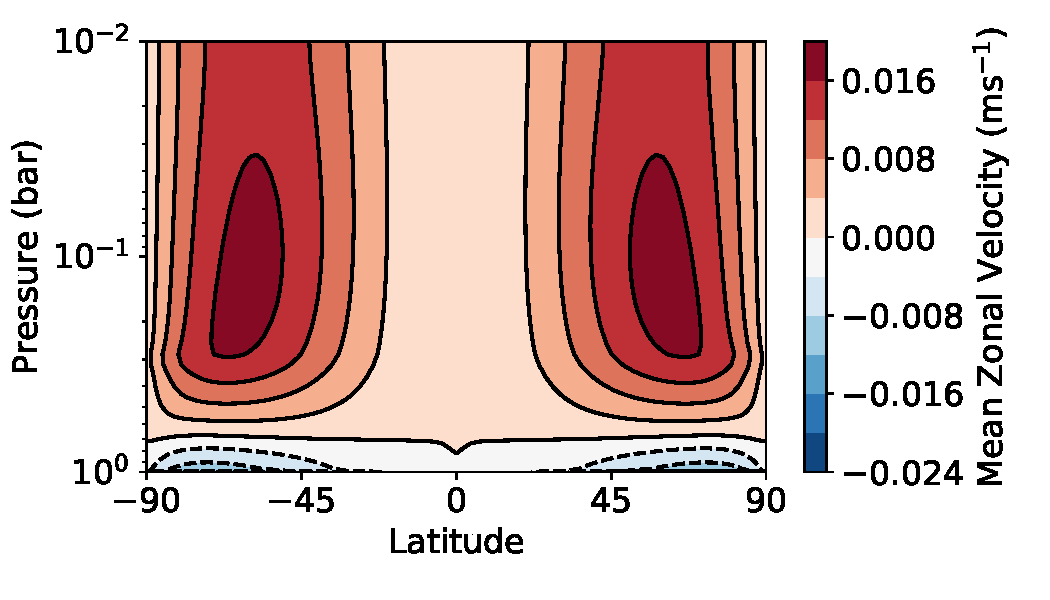
\includegraphics[width=\textwidth]{figures/eqm-zonal-flow/zonal-wind-tide-day1.pdf}
    \caption{1: Zonal velocity.}
  \end{subfigure}
\enskip
  \begin{subfigure}[t]{0.31\textwidth}
    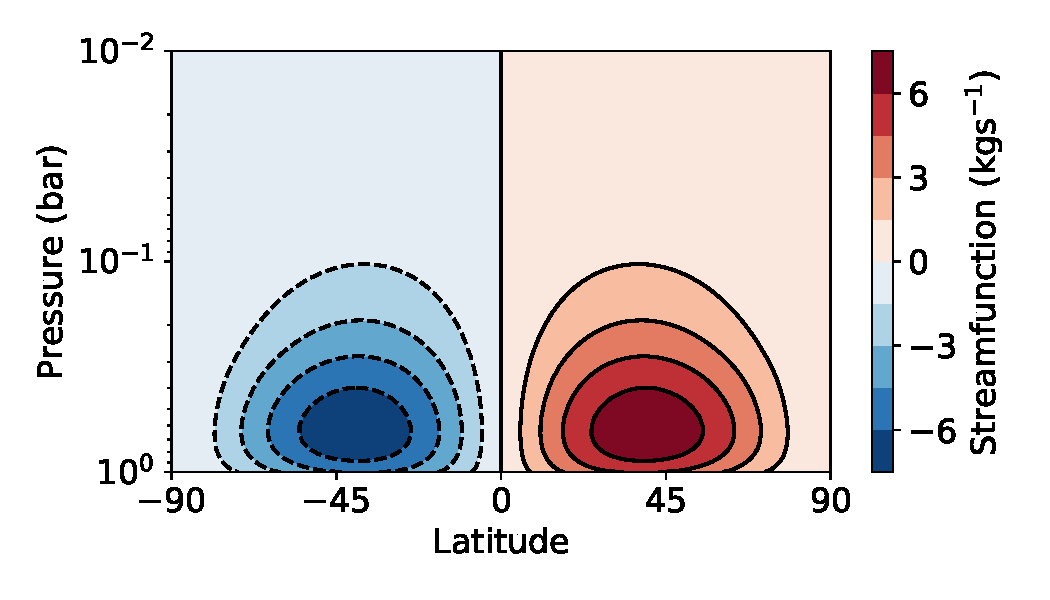
\includegraphics[width=\textwidth]{figures/eqm-zonal-flow/streamfunction-tide-day1.pdf}
    \caption{1: Mass streamfunction.}
  \end{subfigure}
  \\
  \begin{subfigure}[t]{0.31\textwidth}
    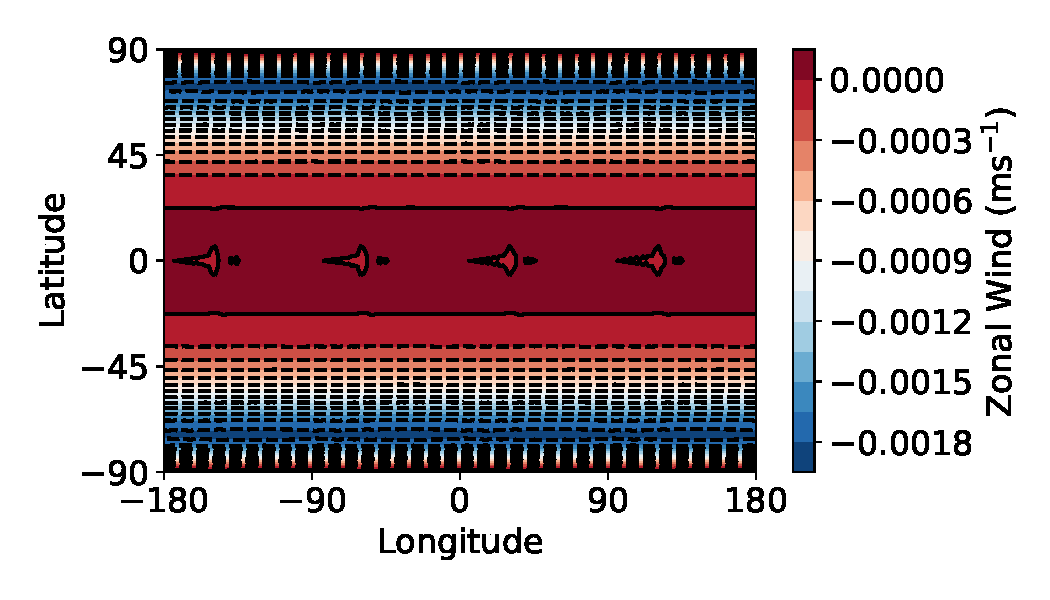
\includegraphics[width=\textwidth]{figures/eqm-zonal-flow/zonal-wind-map-axi-day1.pdf}
    \caption{2: Surface zonal velocity.}
  \end{subfigure}
\enskip
  \begin{subfigure}[t]{0.31\textwidth}
    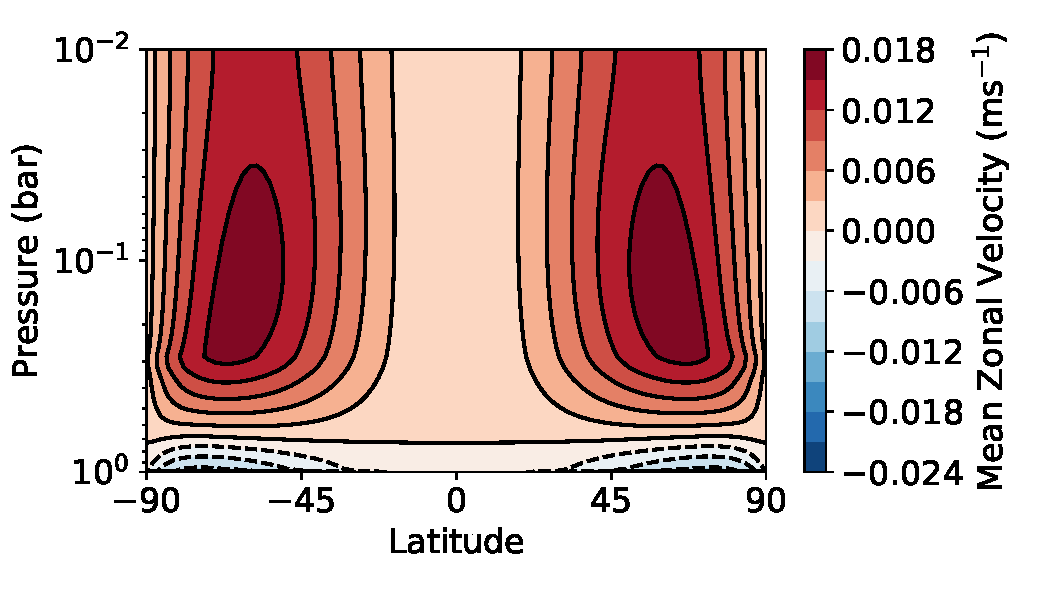
\includegraphics[width=\textwidth]{figures/eqm-zonal-flow/zonal-wind-axi-day1.pdf}
    \caption{2: Zonal velocity.}
  \end{subfigure}
\enskip
  \begin{subfigure}[t]{0.31\textwidth}
    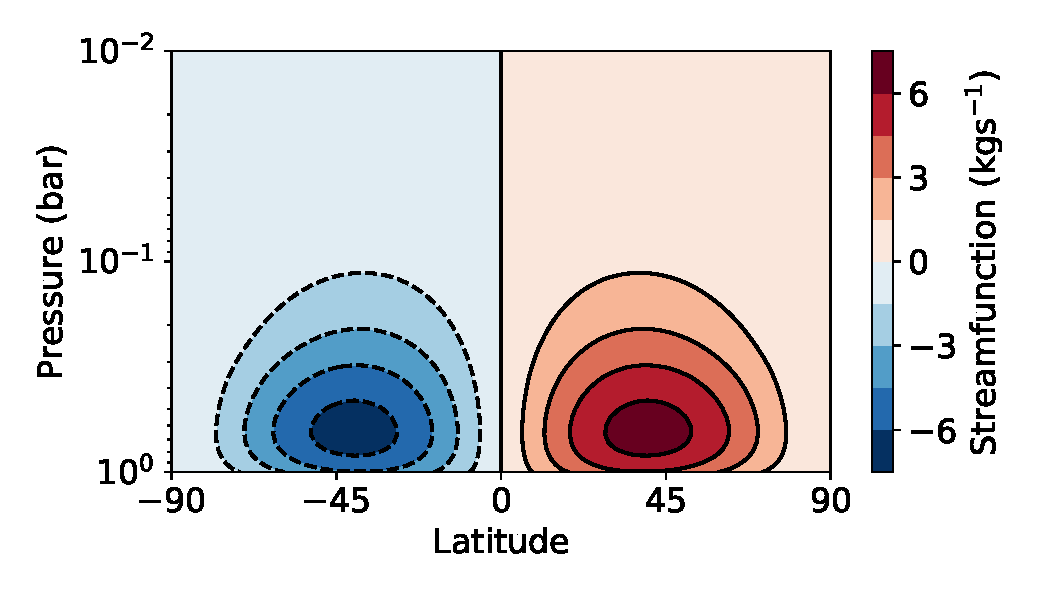
\includegraphics[width=\textwidth]{figures/eqm-zonal-flow/streamfunction-axi-day1.pdf}
    \caption{2: Mass streamfunction.}
  \end{subfigure}
  \caption{Time-mean results from Tests 1 and 2, for the first day after initialisation from rest. The top row shows the tidally locked planet Test 1, and the bottom row shows Test 2, a planet with axisymmetric forcing with the same zonal mean. The zonal mean zonal velocity and mean mass streamfunction are the same in both cases, despite the large differences in the longitudinal distribution of the forcing.}\label{fig:day-1-tide-axi}
\end{figure}



% Following REF(ZG), I impose a background flow $\overline{U}(\phi)$ based on the vorticity profile X.

% Then I linearise the equations X about this flow and calculate the response to forcing X with the method X in Appendix X, then calculate the resulting zonal acceleration from Equation X.

% Figure X shows the solution with an imposed jet X that gives zero zonal acceleration at the equator, with and without the background flow from a mean meridional circulation X. It shows that with the mean meridional circulation, the flow can be prograde at all latitudes (although must be sub-rotating at high latitudes).
%
% Figure X shows a strong meridional circulation with dominant subtropical jets. The pattern matches the circulation in Noda, with two peaks off the equator.




%SUBSECTION -- DEMONSTRATION OF MECHANISM
\subsection{Demonstration of GRW Mechanism}


This section shows the formation of zonal flow in Tests 1 and 2, demonstrating how the GRW mechanism adds angular momentum to the atmosphere in Test 1 and creates eastward flow at all latitudes. The total atmospheric angular momentum is \citep{lebonnois2012momentum}:

\begin{equation}
  M=\int_{V} u a \cos \theta d m
\end{equation}

where $\int_{V}$ is the integral of mass over the whole atmosphere, $u$ is the local zonal velocity, $a$ is the planetary radius, and $\theta$ is the latitude.

Figure \ref{fig:global-m} shows the total atmospheric angular momentum in Test 1 as it spins up from rest. The only source or sink of angular momentum apart from numerical error is the linear Rayleigh drag applied to the winds in the boundary layer near the surface. It gains angular momentum as the surface drags the winds in the boundary layer, then reaches equilibrium when there is sufficient eastward wind and westward torque for no net effect. The total angular momentum varies over a period of hundreds of days, with fluctuations that are small compared to the large variability in the angular momentum of similar simulations of superrotation on Venus \citep{lebonnois2012momentum}.

% Test 1 reaches equilibrium at a greater total angular momentum than Test 2, which may be due to the equatorward momentum transport reducing the eastward momentum transported to the surface by the meridional circulation, so allowing a greater eastward flow in the upper branch before the boundary layer winds reach zero net drag.

Figure \ref{jet-layer-m} shows the angular momentum in Test 1 in the model level of the maximum zonal-mean zonal flow. The angular momentum in this level increases as the model spins up, then reaches a positive value at equilibrium. This contradicts the shallow-water model in \citet{showman2011superrotation} which loses angular momentum from the level of the jet. The positive net angular momentum is explained by the GRW mechanism, which transports angular momentum from the surface to the atmosphere, and to the upper branch of the meridional circulation.

\begin{figure}
  \centering
  \begin{subfigure}[t]{0.48\textwidth}
    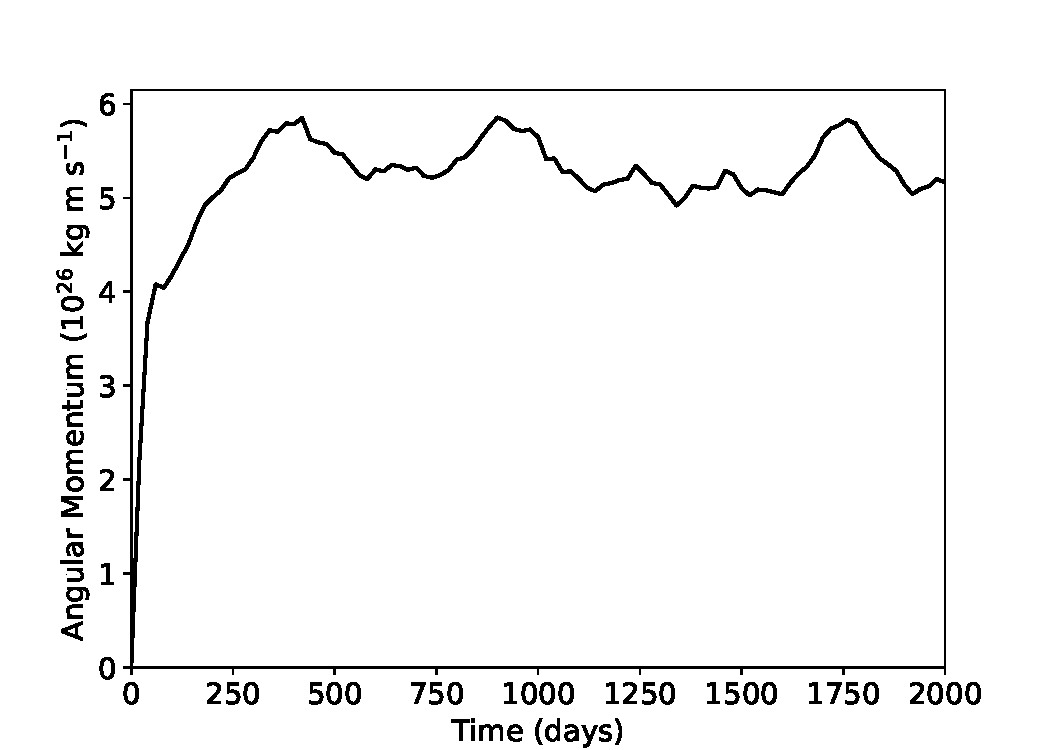
\includegraphics[width=1.0\textwidth]{figures/eqm-zonal-flow/global-m.pdf}
    \caption{Total angular momentum.}\label{fig:global-m}
  \end{subfigure}
\quad
  \begin{subfigure}[t]{0.48\textwidth}
    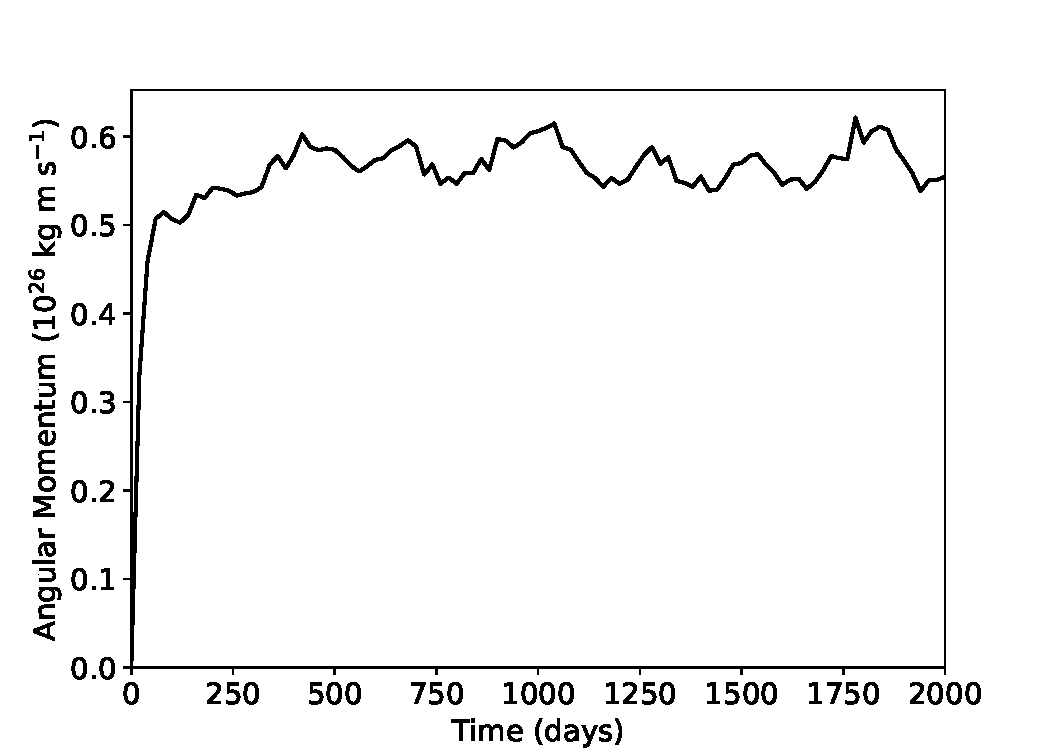
\includegraphics[width=1.0\textwidth]{figures/eqm-zonal-flow/jet-layer-m.pdf}
    \caption{Angular momentum in the jet layer.}\label{jet-layer-m}
  \end{subfigure}
  \caption{The spin-up in Test 1 of angular momentum globally and at the pressure level where the jet is strongest, showing how both regions gain momentum over time then equilibrate.}\label{fig:global-jet-layer-m-spinup}
\end{figure}

Figures \ref{fig:test-1-spinup} and \ref{fig:test-2-spinup} show the development of the zonal flow in Tests 1 and 2. Figure \ref{fig:test-2-spinup} shows the evolution of the flow in Test 2, where subtropical jets form immediately due to the mean meridional circulation, then strengthen and reach equilibrium. Figure \ref{fig:test-1-spinup} shows that the same subtropical jets form initially in Test 1, but then the stationary waves transport angular momentum towards the equator \citep{showman2011superrotation}. Test 1 reaches an equilibrium state with a single equatorial jet and eastward flow at high latitudes due to acceleration from the meridional circulation.



% The first row of Figure \ref{fig:test-1-2-spinup} shows the development of the zonal-mean zonal wind as it spins up from rest in the axisymmetric case, Test 2. The forcing gradient between the equator and the pole results in a mean meridional circulation that rapidly produces subtropical jets, which strengthen with time until they reach equilibrium. Note that there is no eastward flow at the equator, and the superrotation index is negative everywhere as there is no process to transport momentum equatorward.
%
% The second row of Figure \ref{fig:test-1-2-spinup} shows the development of the zonal-mean zonal wind as it spins up from rest in the tidally locked case, Test 1. The first panel shows that exactly the same subtropical jets form at the start of the spin-up as in the axisymmetric case, due to the linear response as explained previously. In the next panel, the stationary waves induced by the stationary forcing transport momentum towards the equator, producing eastward superrotating flow there. This weakens the subtropical jets, but they are still present at high latitudes. In the final panel, the equatorward transport has produced a strong single equatorial jet, with no distinct subtropical jets present. The balance between these the equatorward transport and the mean meridional circulation determines the relative strength of the equatorial and subtropical jets, which I will investigate in more detail later.

\begin{figure}
  \centering
  \begin{subfigure}[t]{0.31\textwidth}
    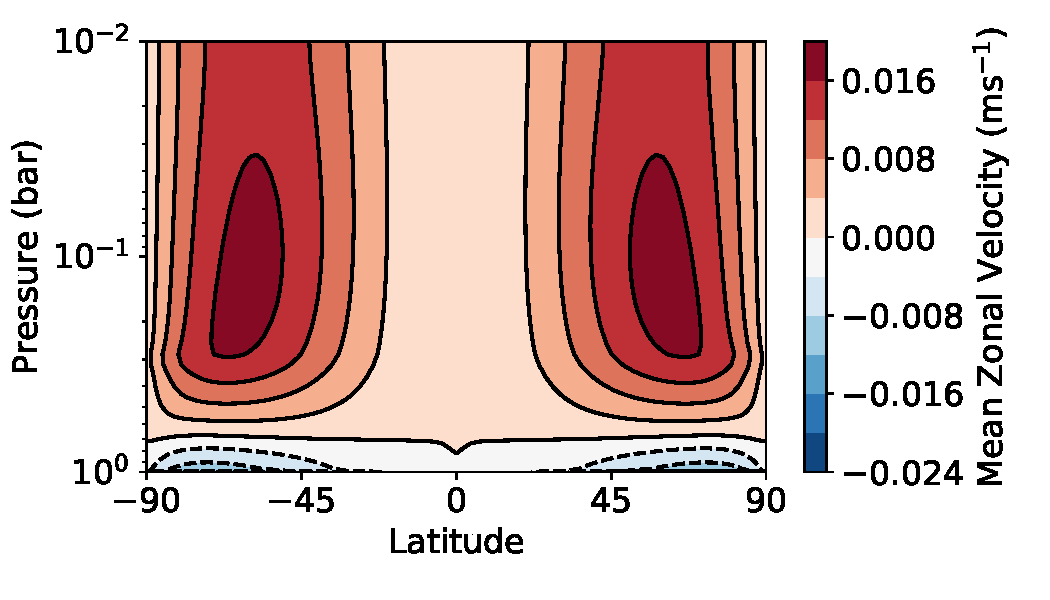
\includegraphics[width=\textwidth]{figures/eqm-zonal-flow/zonal-wind-tide-day1.pdf}
    \caption{Day 1.}
  \end{subfigure}
\enskip
  \begin{subfigure}[t]{0.31\textwidth}
    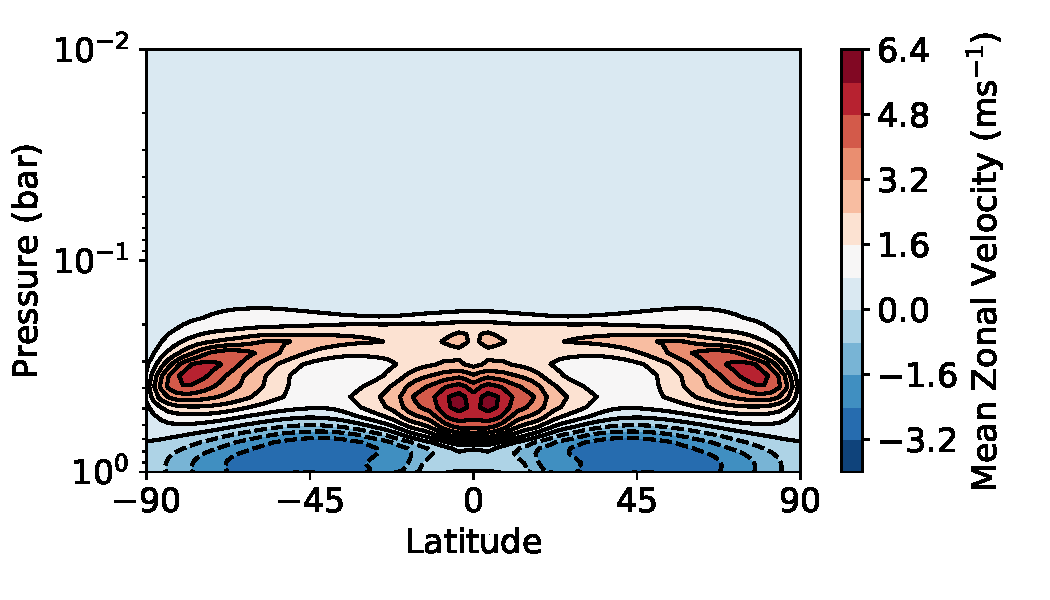
\includegraphics[width=\textwidth]{figures/eqm-zonal-flow/tl-zonal-u-5day.pdf}
    \caption{Day 5.}
  \end{subfigure}
\enskip
  \begin{subfigure}[t]{0.31\textwidth}
    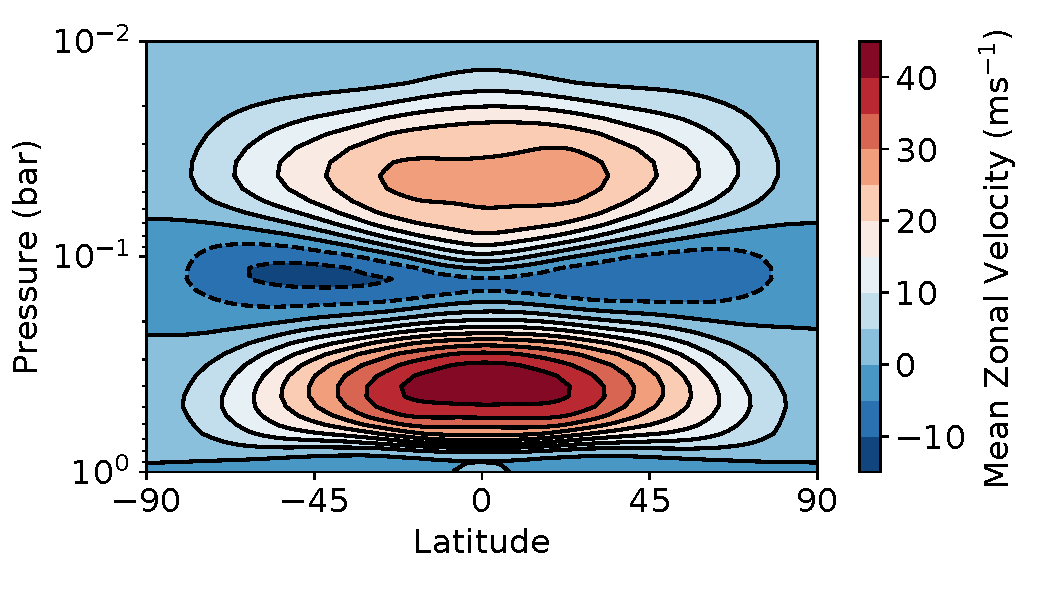
\includegraphics[width=1.0\textwidth]{figures/eqm-zonal-flow/default-gcm-zonal-flow.pdf}
    \caption{1000 to 2000 days.}
  \end{subfigure}
  \caption{The zonal-mean zonal velocity of the tidally locked planet in Test 1 as it spins up from rest, forming subtropical jets before the equatorward momentum transport produces the equatorial jet. The time-mean fields on day 1, on day 5, and from day 1000 to 2000 are plotted.}\label{fig:test-1-spinup}
\end{figure}


\begin{figure}
  \centering
  \begin{subfigure}[t]{0.31\textwidth}
    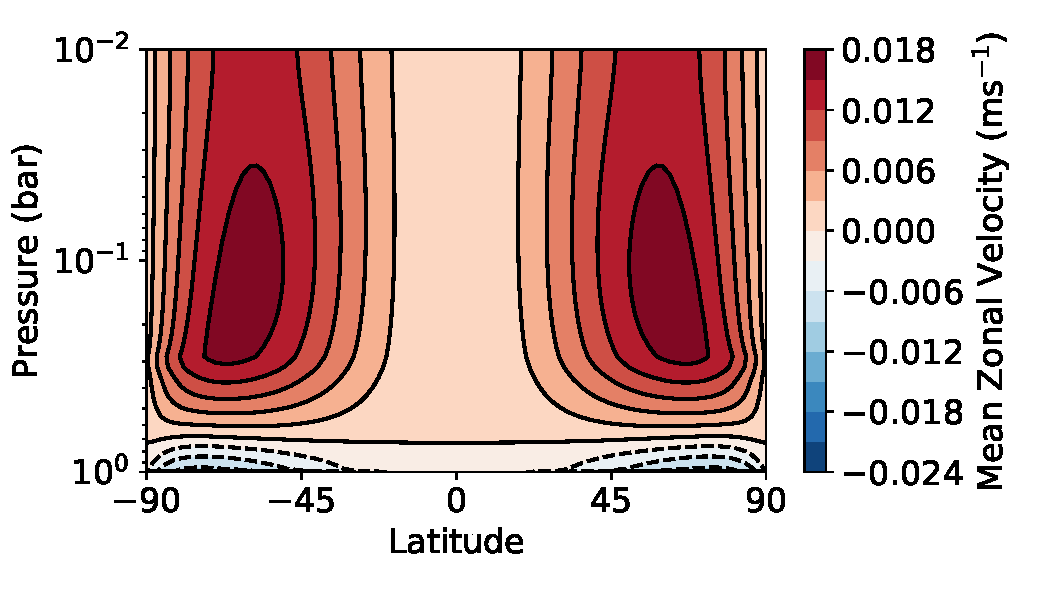
\includegraphics[width=\textwidth]{figures/eqm-zonal-flow/zonal-wind-axi-day1.pdf}
    \caption{Day 1.}
  \end{subfigure}
\enskip
  \begin{subfigure}[t]{0.31\textwidth}
    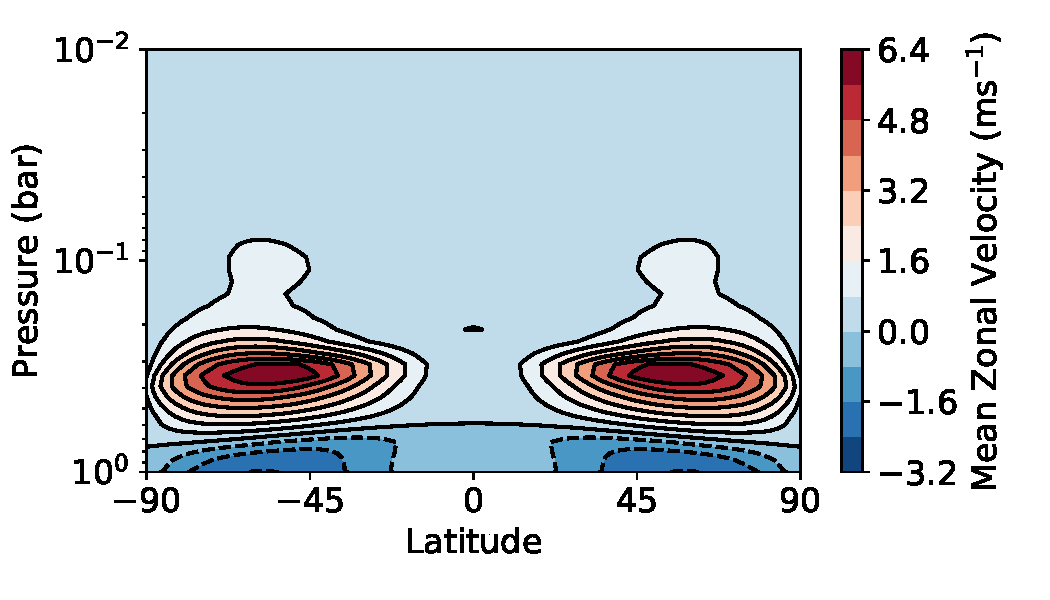
\includegraphics[width=\textwidth]{figures/eqm-zonal-flow/axi-zonal-u-5day.pdf}
    \caption{Day 5.}
  \end{subfigure}
\enskip
  \begin{subfigure}[t]{0.31\textwidth}
    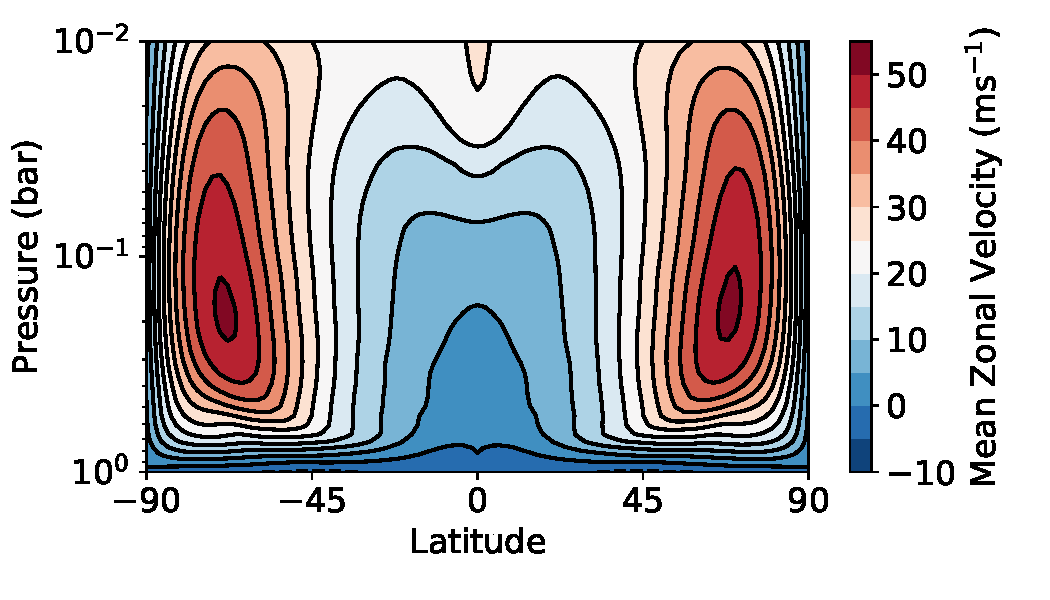
\includegraphics[width=1.0\textwidth]{figures/eqm-zonal-flow/default-gcm-axi-zonal-flow.pdf}
    \caption{1000 to 2000 days.}
  \end{subfigure}
  \caption{The zonal-mean zonal velocity of the axisymmetrically forced planet in Test 2 as it spins up from rest, forming subtropical jets. The time-mean fields on day 1, on day 5, and from day 1000 to 2000 are plotted.}\label{fig:test-2-spinup}
\end{figure}



%
% Figure \ref{fig:default-gcm-velocity-drag} shows the time-mean zonal-mean zonal velocity and the resulting drag for Test 1 from 500 to 1500 days (the same as the final panel of \ref{fig:test-1-2-spinup}). The second panel shows the effect of the linear Rayleigh drag applied in the boundary layer, which decays linearly with pressure away from the surface to zero at $70 \%$ of the surface pressure. There is a positive westerly acceleration due to drag at the surface due to the surface easterlies formed by the mean meridional circulation. This drag pumps prograde momentum into the atmosphere, which is responsible for the increase in angular momentum during spin-up shown by Figure \ref{fig:global-jet-layer-m-spinup}.



\subsection{Zonal Momentum Fluxes}

This section shows that the GRW mechanism explains the equilibrium zonal momentum budget in Test 1. The steady-state zonal-mean momentum equation is \citep{lutsko2018response}:

\begin{equation}\label{eqn:zonal-mean-mom-gcm}
  \begin{split}
    \frac{\partial \overline{u}}{\partial t} = \underbrace{f[\overline{v}]-\frac{[\overline{v}]}{a \cos \phi} \frac{\partial}{\partial \phi}([\overline{u}] \cos \phi)}_{Ia}
    \underbrace{-[\overline{\omega}] \frac{\partial[\overline{u}]}{\partial p}}_{Ib} \\
    \underbrace{-\frac{1}{a \cos ^{2} \phi} \frac{\partial}{\partial \phi}\left(\left[\overline{u}^{\prime} \overline{v}^{\prime}\right] \cos ^{2} \phi\right)}_{IIa}
    \underbrace{-\frac{\partial}{\partial p}\left[\overline{u}^{\prime} \overline{\omega}^{\prime}\right]}_{IIb}
    \underbrace{+\left[\overline{F_{x}}\right]}_{III} \end{split}
\end{equation}

where $\omega$ is the vertical velocity, and all other variables are the same as before. Terms Ia and Ib are the mean horizontal and vertical momentum transport due to the mean meridional circulation. Term IIa is the eddy horizontal momentum transport from the stationary wave response to the stellar forcing, and Term IIb is the eddy vertical momentum transport due to vertical motion. This vertical motion is mostly due to air rising at the substellar point and subsiding on the night-side. Term III is the forcing applied to the zonal winds, which in this case is the Rayleigh drag in the boundary layer near the surface.

Figure \ref{fig:default-gcm-accelerations} shows each of the momentum transport terms in Equation \ref{eqn:zonal-mean-mom-gcm}. Term Ia is plotted in Figure \ref{fig:mean-horiz}, which shows how the mean meridional circulation produces an acceleration in the midlatitudes in its poleward branch and has no effect at the equator. There is a westward acceleration at the surface due to the lower branch of the mean meridional circulation. This produces the westward surface flow that results in an eastward torque on the atmosphere from the Rayleigh drag in the boundary layer.

Figure \ref{fig:mean-vert} shows Term Ib, where the primary effect is the ascending branch of the mean meridional circulation moving the equatorial jet upwards, as shown by the deceleration below the centre of the jet and the acceleration above the centre of the jet. This term has zero effect where there is zero vertical gradient in the mean zonal flow, so it does not affect the maximum zonal flow at the centre of the jet, and is not as important as the other terms to the equilibrium state.

Figure \ref{fig:stat-horiz} plots Term IIa, and shows how the stationary waves excited by the stellar forcing transport eastward momentum horizontally towards the equator. This produces an acceleration at the equator and a deceleration at higher latitudes. Term IIb in Figure \ref{fig:stat-vert} shows how the vertical momentum transport decelerates the jet. It moves stationary air up on the day-side, reducing the specific westerly angular momentum of the jet. There is an additional deceleration on the jet from the subsiding air on the night-side moving eastward angular momentum down and out of the jet layer. This produces eastward flow at the surface, which results in a westward drag that opposes the eastward drag on the lower branch of the meridional circulation, resulting eventually in equilibrium.


Figure \ref{fig:accn-terms-jet-level} shows each term in Figure \ref{fig:default-gcm-accelerations} at \SI{0.3}{\bar}, near the centre of the jet. It shows that the Terms Ia and IIa balance at high latitudes, and that Term IIb balances Term IIa at the equator, as shown in the linear model in Figure \ref{fig:beta-fluxes-plus-merid}. Terms Ia and IIa become weak at very high latitudes, unlike the shallow-water model in Figure \ref{fig:test-C-accn} where both terms are strong almost until the pole. This is because the meridional circulation does not extend all the way to the pole in the GCM, unlike in the idealised shallow-water model. The balance of fluxes governing the equilibrium flow is still the same in both models.

\begin{figure}
  \centering
  \begin{subfigure}[t]{0.48\textwidth}
    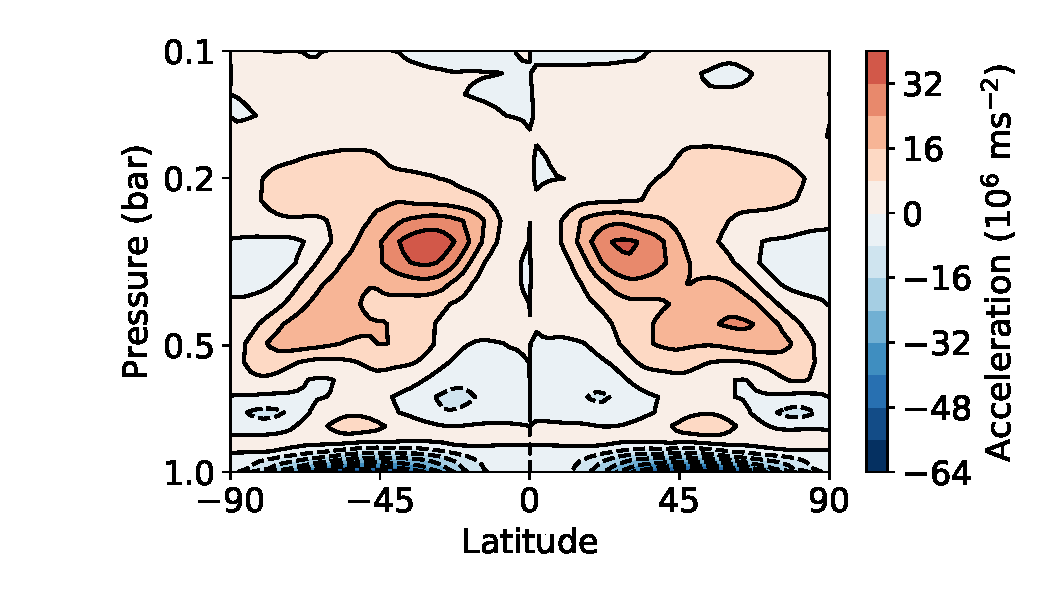
\includegraphics[width=\textwidth]{figures/eqm-zonal-flow/0_flux.pdf}
    \caption{Term Ia, Mean Horizontal.}\label{fig:mean-horiz}
  \end{subfigure}
\quad
  \begin{subfigure}[t]{0.48\textwidth}
    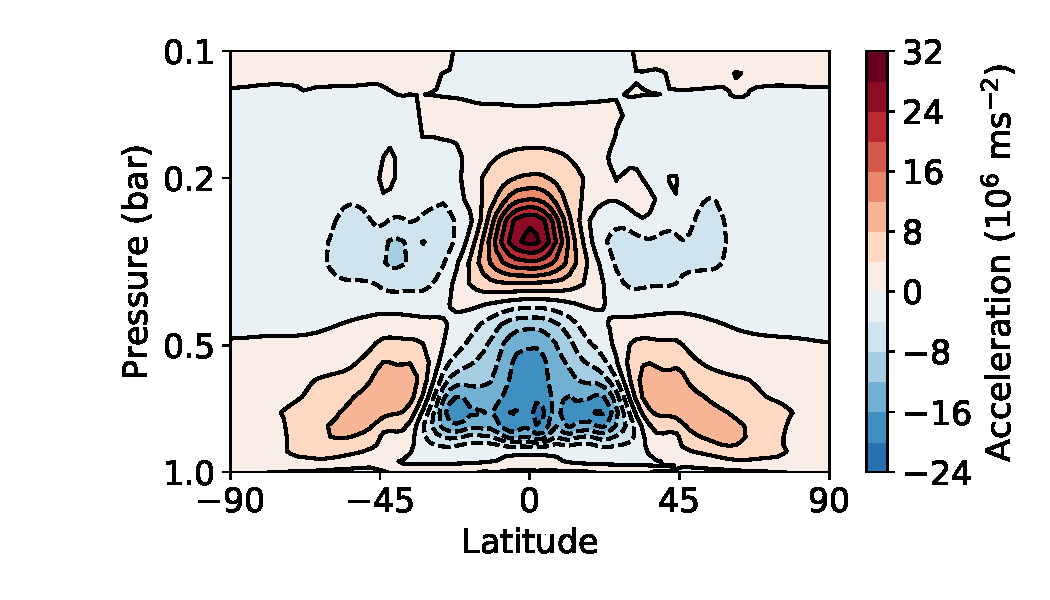
\includegraphics[width=\textwidth]{figures/eqm-zonal-flow/1_flux.pdf}
    \caption{Term Ib, Mean Vertical.}\label{fig:mean-vert}
  \end{subfigure}
  \\
  \begin{subfigure}[t]{0.48\textwidth}
    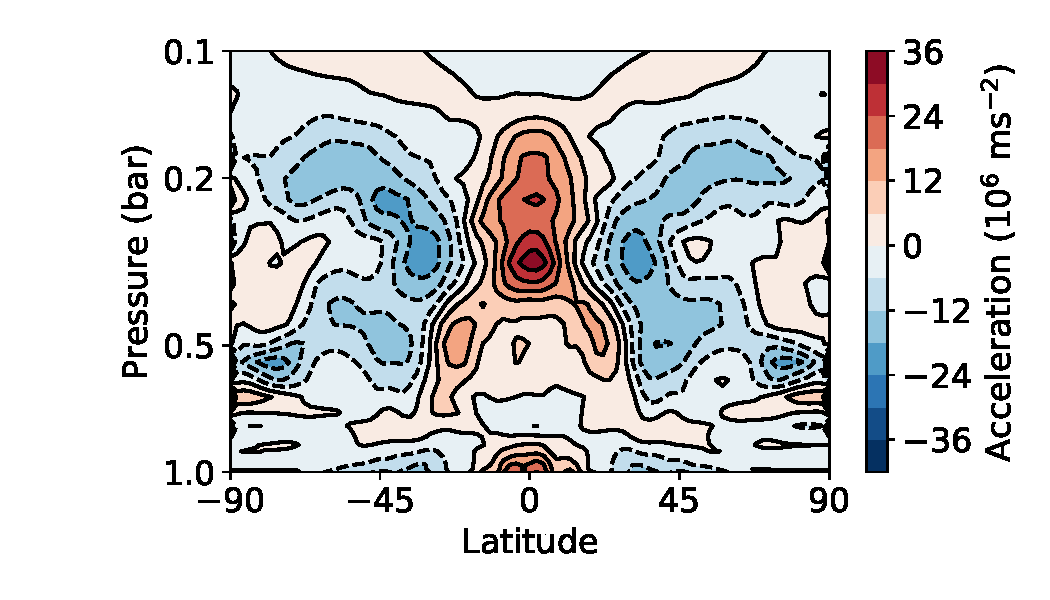
\includegraphics[width=\textwidth]{figures/eqm-zonal-flow/2_flux.pdf}
    \caption{Term IIa, Eddy Horizontal.}\label{fig:stat-horiz}
  \end{subfigure}
\quad
  \begin{subfigure}[t]{0.48\textwidth}
    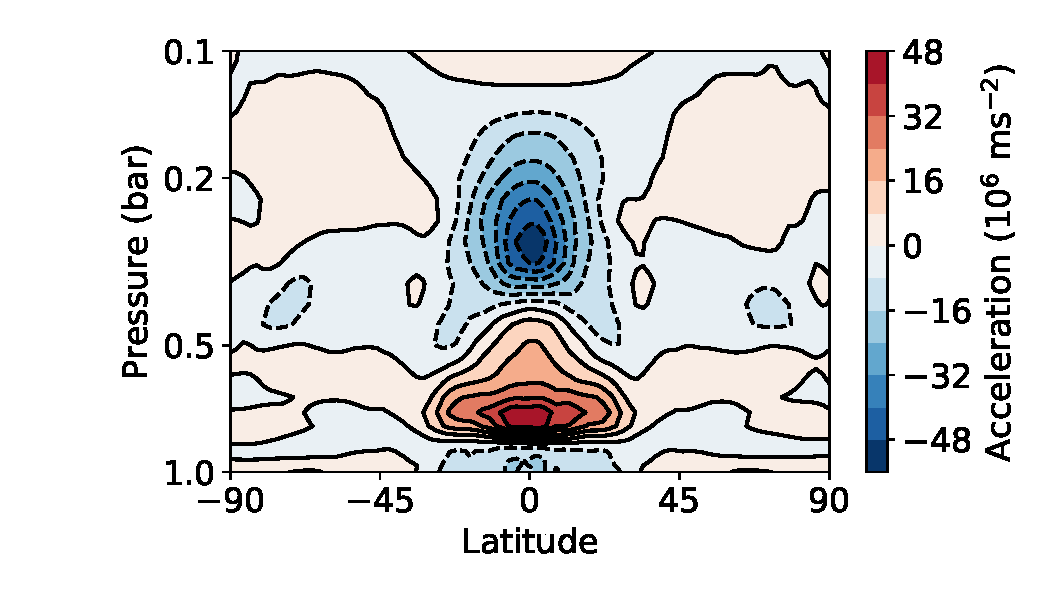
\includegraphics[width=\textwidth]{figures/eqm-zonal-flow/3_flux.pdf}
    \caption{Term IIb, Eddy Vertical.}\label{fig:stat-vert}
  \end{subfigure}
  \caption{The sources of zonal acceleration in Equation \ref{eqn:zonal-mean-mom-gcm}, showing how different terms accelerate and decelerate zonal flow at the equator and at high latitudes. Figure \ref{fig:accn-terms-jet-level} plots these terms at \SI{0.3}{\bar}. }\label{fig:default-gcm-accelerations}
\end{figure}


The ``Mean Vertical'' acceleration of Term Ib is also different to the shallow-water models. It contributes to the eastward acceleration at the equator, opposing Term IIb. This appears to be different to the fluxes in the shallow-water models, where the mean vertical acceleration has no effect. However, Figure \ref{fig:mean-vert} showed that the mean vertical acceleration has a negligible net effect on the strength of the jet, with an acceleration above its centre but a deceleration below its centre. This means that it has no net effect on the strength of the jet, so does not need to be considered when comparing to the single-layer shallow-water models. The balance of acceleration terms in Figure \ref{fig:accn-terms-jet-level} for the GCM is therefore qualitatively the same as the balance of terms in Figure \ref{fig:test-C-accn} for the non-linear shallow-water model, matching the GRW mechanism.

%
% Comparing this to Figure \ref{fig:test-3-accn} shows that the same balance applies in Test C in the non-linear shallow-water model as in Test 1 in the GCM. I suggest that this agreement between the non-linear shallow-water model and the GCM shows that the shallow-water model captures the mechanism forming the zonal flow profile in the GCM. This shows that the important processes in the atmosphere can be split up into the wave-1 day-night forcing, and the wave-0 zonal-mean forcing due to the asymmetry between the day-side cooling and uniform night-side cooling. In the next section, I will use a non-linear shallow-water model to reproduce this process, and show that the same balance of acceleration terms applies.



% \begin{figure}
%   \centering
%   \begin{subfigure}[t]{0.48\textwidth}
%     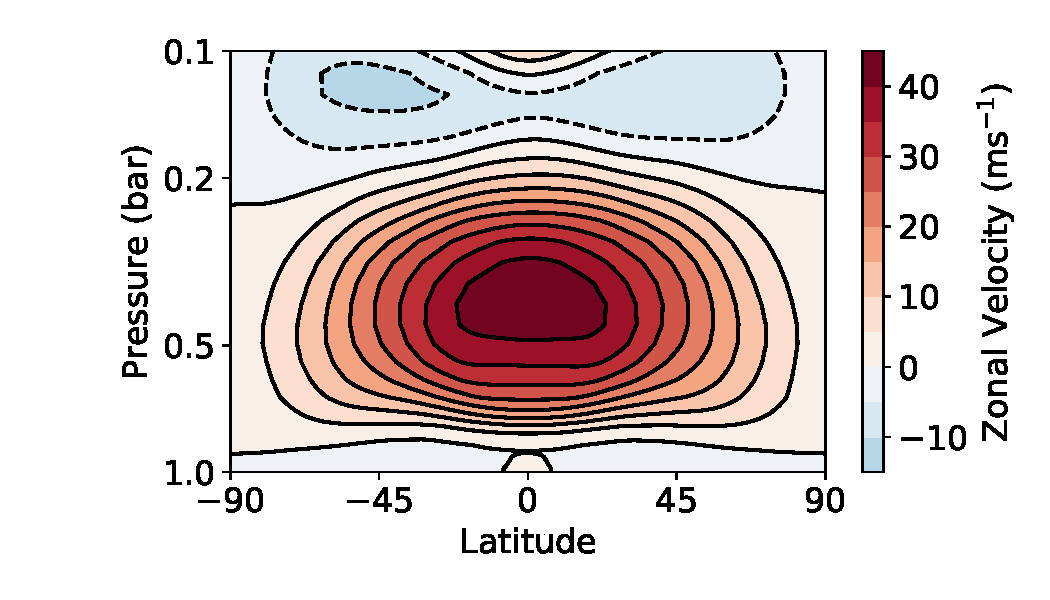
\includegraphics[width=\textwidth]{figures/eqm-zonal-flow/5_flux.pdf}
%     \caption{Zonal-mean zonal velocity.}
%   \end{subfigure}
% \quad
%   \begin{subfigure}[t]{0.48\textwidth}
%     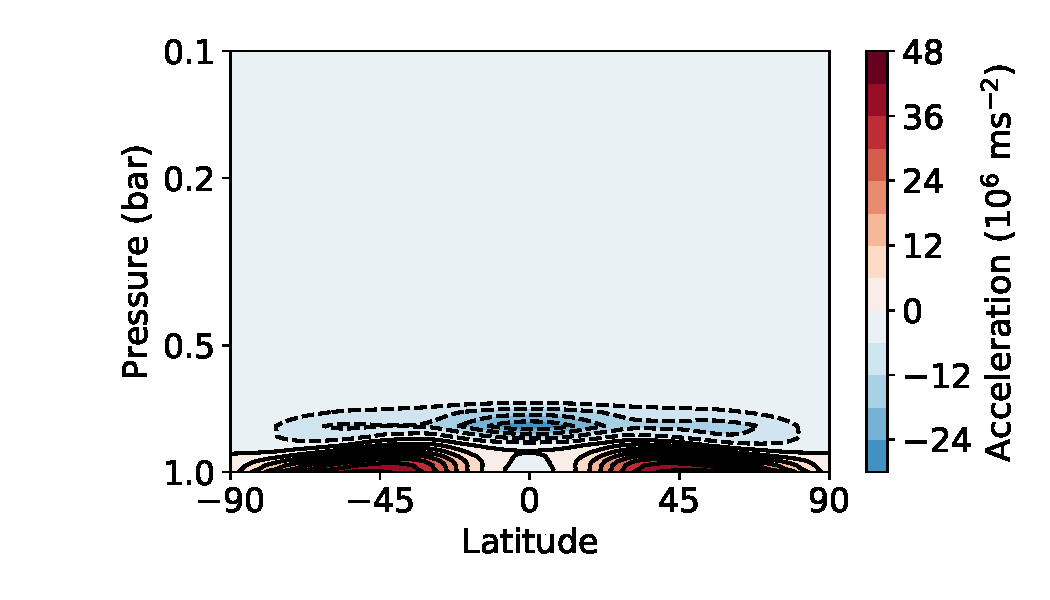
\includegraphics[width=\textwidth]{figures/eqm-zonal-flow/4_flux.pdf}
%     \caption{Acceleration due to Rayleigh drag.}
%   \end{subfigure}
%   \caption{Zonal velocity and drag}
%   \label{fig:default-gcm-velocity-drag}
% \end{figure}



\begin{figure}
  \centering
  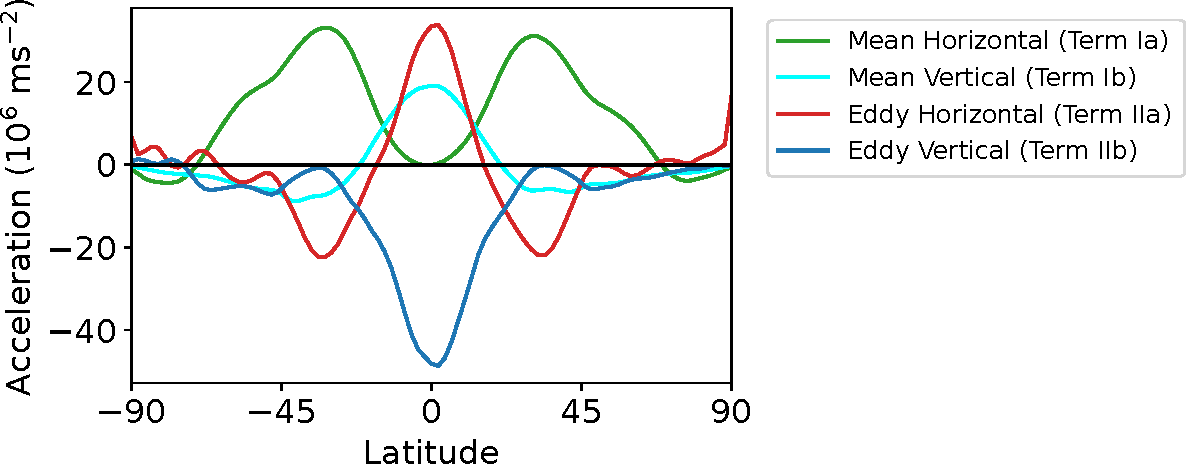
\includegraphics[width=0.9\textwidth]{figures/eqm-zonal-flow/accn-terms-jet-level.pdf}
  \caption{Acceleration terms in the zonal-mean zonal momentum equation at \SI{0.3}{\bar} in Test 1 in Exo-FMS, showing how Terms Ia and IIa in Equation \ref{eqn:zonal-mean-mom-gcm} balance at high latitudes, and that Term IIb balances Terms IIa and Ib at the equator. This matches the shallow-water models in Figures \ref{fig:beta-fluxes-plus-merid} and \ref{fig:test-C-accn}, except for the presence of Term Ib, which is explained in the text.}\label{fig:accn-terms-jet-level}
\end{figure}


%SECTION CONCLUSIONS



%%%%%%%%%%%%%%%%%%%%%%%%%%%%
%SECTION 4 -- SCALING REGIMES
\section{Scaling Behaviour of Zonal Jets on Tidally Locked Planets}

In this section, I will use the ideas developed so far to predict how the strengths and positions of the zonal jets in the atmospheres of tidally locked planets could scale with planetary parameters. \citet{perez2013atmospheric} use a similar non-linear model to derive scaling relations for the global height field and associated day-night contrast. This section will focus on the scaling behaviour of the strength and position of the jets formed on tidally locked planets.


%SUBSECTION -- NONLINEAR MODEL
\subsection{Non-Linear Model Scaling Relations}\label{sec:nonline-scaling-relations}

Equation \ref{eqn:zonal-mean-mom-sphere} shows how each source of acceleration scales with the planetary parameters. Term II drives the equatorial jet, suggesting that the jet speed should scale like $\frac{1}{\overline{h}} \frac{\partial}{\partial y}\left[\overline{(h v)^{\prime} u^{\prime}}\right] \sim u^{\prime} v^{\prime} \sim Q^{2}\alpha^{2}$. Term I in Equation \ref{eqn:zonal-mean-mom-sphere} drives the subtropical jets, suggesting that they should scale like $\overline{v}^{\star}\left[f-\frac{\partial \overline{u}}{\partial y}\right] \sim v^{\prime} f \sim Q\alpha f$.

Figure \ref{fig:u_Q_scaling} shows the scaling of the zonal-mean equatorial and subtropical jet speeds with the forcing strength $\delta h$. Each test has the same parameters as Test C in Section \ref{sec:nonlin-shallow}, except for the magnitude of the forcing. The figure shows that for low forcing values, the equatorial jet does scale quadratically with the forcing (as identified by \citet{showman2011superrotation}), and the subtropical jets scale linearly. For forcing values higher than $\Delta h / h_{0} = 0.01$, the jets increases more slowly than linearity, as non-linear effect become more important. For realistic forcing values of order 0.01 \citep{showman2011superrotation}, the jets still obey this linear scaling trend.

% This test shows that the accelerations of the jets scale as expected in the linear limit, and that the magnitude of forcing required for an approximately linear response is still consistent with that in \citet{showman2011superrotation}.

This predicts that increasing the forcing (instellation) on a tidally locked planet will increase both the equatorial and subtropical jet speeds, and will increase the equatorial jet speed relative to the subtropical jets. In addition, the equatorial acceleration comes at the expense of the subtropical jets due to the equatorward momentum transport, so for very strong forcing the subtropical jets may be replaced by easterly flow.

% Figure \ref{fig:u_Q_scaling} shows the scaling of the zonal-mean equatorial and subtropical jet speeds with damping $\alpha$. Equation \ref{eqn:zonal-mean-mom-sphere} suggests that the equatorial jet should scale quadratically with $\alpha$, and that the subtropical jets should scale linearly. As with the forcing, these behaviour holds up to a value X where the jets increase more slowly with the damping rate. Still realistic X.

% In the next section, I will consider similar scaling relations in the GCM.


\begin{figure}
  \centering
    \includegraphics[width=0.8\textwidth]{figures/eqm-zonal-flow/u_Q_scaling.pdf}
  \caption{The equatorial and subtropical jet speeds in the non-linear shallow-water model, versus the magnitude $Q = \delta h /h_{0}$ of the realistic forcing field in Test C, where $h_{0} =$ \SI{1e4}{\metre}. The lines show fits of the predicted quadratic scaling of the equatorial jet, and linear scaling of the subtropic jets.}
  \label{fig:u_Q_scaling}
\end{figure}

% \begin{figure}
%   \centering
%   \begin{subfigure}[t]{0.49\textwidth}
%     \includegraphics[width=1.0\textwidth]{figures/eqm-zonal-flow/u_Q_scaling.pdf}
%     \caption{Effect of forcing magnitude $Q$.}
%     \label{fig:u_Q_scaling}
%   \end{subfigure}
%   %
%   \begin{subfigure}[t]{0.49\textwidth}
%     \includegraphics[width=1.0\textwidth]{figures/eqm-zonal-flow/u_alpha_scaling.pdf}
%     \caption{Effect of radiative damping $\alpha$.}
%     \label{fig:u_alpha_scaling}
%   \end{subfigure}
%   \caption{The scaling of the equatorial and subtropical jet speeds in the non-linear shallow-water model, for cases with realistic forcing with variable values of forcing magnitude $Q$ and radiative damping $\alpha$.}
%   \label{fig:nonlin-scaling}
% \end{figure}


%SUBSECTION -- GCM
\subsection{Qualitative GCM Scaling Relations}\label{fig:gcm-qual-scaling}

This section will qualitatively apply the scaling relations from the non-linear shallow-water model to a suite of GCM simulations. Figure \ref{fig:gcm-suite-jets} shows the zonal-mean zonal velocity of nine GCM simulations with different rotation rates and instellation values, adapted from \citet{pierrehumbert2018review}. These tests have a range of zonal flow patterns, with one, two, or three jets of varying strengths and positions, which can be explained with the scaling relations of the previous section.

 Increasing the instellation in the GCM increases the forcing $Q$, and raises the damping rate $\alpha$ due to the higher temperature. I showed previously that increasing the forcing $Q$ and damping $\alpha$ in the shallow-water model increases the strength of all the zonal jets, and increases the strength of the equatorial jet relative to the subtropical jets. This explains why the GCM tests with higher instellation have strong, single equatorial jets, with all the ``hot'' tests having one single jet centred on the equator. The ``hot, 2 day'' test has easterly flow at high latitudes, as the high forcing increases the prograde momentum transport towards the equator.

The GRW mechanism predicts that increasing the rotation rate of the planet should strengthen the subtropical jets, and move them to lower latitudes. This is confirmed by the GCM tests, and is shown most clearly by the ``cold'' cases, where increasing the rotation rate gives faster jets than are closer together. In the ``hot'' simulations, the subtropical jets merge with the equatorial jet and there appears to only be one jet. The GRW mechanism therefore explains the qualitative behaviour of this suite of simulations, and provides an understanding of why GCM simulations of the atmospheres of tidally locked terrestrial planets can have one, two, or three zonal jets of varying strengths.


\begin{figure}
  \centering
  \begin{subfigure}[b]{0.32\textwidth}
    \includegraphics[width=\textwidth]{figures/eqm-zonal-flow/wind-hot-10.pdf}
    \caption{Hot, 10 days.}
  \end{subfigure}
  \begin{subfigure}[b]{0.32\textwidth}
    \includegraphics[width=\textwidth]{figures/eqm-zonal-flow/wind-med-10.pdf}
    \caption{Medium, 10 days.}
  \end{subfigure}
  \begin{subfigure}[b]{0.32\textwidth}
    \includegraphics[width=\textwidth]{figures/eqm-zonal-flow/wind-cold-10.pdf}
    \caption{Cold, 10 days.}
  \end{subfigure}
    \\
    \begin{subfigure}[b]{0.32\textwidth}
      \includegraphics[width=\textwidth]{figures/eqm-zonal-flow/wind-hot-5.pdf}
      \caption{Hot, 5 days.}
    \end{subfigure}
    \begin{subfigure}[b]{0.32\textwidth}
      \includegraphics[width=\textwidth]{figures/eqm-zonal-flow/wind-med-5.pdf}
      \caption{Medium, 5 days.}
    \end{subfigure}
    \begin{subfigure}[b]{0.32\textwidth}
      \includegraphics[width=\textwidth]{figures/eqm-zonal-flow/wind-cold-5.pdf}
      \caption{Cold, 5 days.}
    \end{subfigure}
     \\
     \begin{subfigure}[b]{0.32\textwidth}
       \includegraphics[width=\textwidth]{figures/eqm-zonal-flow/wind-hot-2.pdf}
       \caption{Hot, 2 days.}
     \end{subfigure}
     \begin{subfigure}[b]{0.32\textwidth}
       \includegraphics[width=\textwidth]{figures/eqm-zonal-flow/wind-med-2.pdf}
       \caption{Medium, 2 days.}
     \end{subfigure}
     \begin{subfigure}[b]{0.32\textwidth}
       \includegraphics[width=\textwidth]{figures/eqm-zonal-flow/wind-cold-2.pdf}
       \caption{Cold, 2 days.}
     \end{subfigure}
  \caption{Time-mean zonal-mean zonal flow of a suite of tests in the GCM Exo-FMS, showing how the equatorial and subtropical jet speeds and positions depend on instellation and rotation rate. Reproduced with data from \citet{pierrehumbert2018review}.}
  \label{fig:gcm-suite-jets}
\end{figure}

% %SUBSECTION -- GCM
% \subsection{GCM Quantitative Scaling Relations}\label{fig:gcm-quant-scaling}
%
% TO DO


%SECTION CONCLUSIONS



%%%%%%%%%%%%%%%%%%%%%%%%%%%%
%DISCUSSION
\section{Discussion}

This section discusses some complicating aspects of applying the GRW mechanism to real tidally locked planets. The GRW mechanism in Figure \ref{fig:gierasch} assumes that the meridional circulation is global, transporting air from the equator to the pole. This is not the case for a rapidly rotating planet like the Earth, which contains multiple cells of meridional circulation. If a tidally locked planet rotated rapidly enough to limit the meridional extent of these cells, the GRW mechanism might only operate below a certain latitude. This may be the case in the more rapidly rotating tests in Figure \ref{fig:gcm-qual-scaling}, where the subtropical jets are closer to the equator and there is easterly flow at high latitudes. However, these tests show that a global meridional circulation is not strictly necessary for the GRW mechanism to function. A limited meridional circulation still receives westerly angular momentum from the surface and conveys it to the jet layer. The subtropical jets will be closer to the equator, and the behaviour at high latitudes may be different.

The meridional circulation is more complicated on tidally locked gas giants like hot Jupiters, which do not have a surface to bound the meridional circulation and apply drag to its lower branch. \citet{heng2011atmospheric} and \citet{mendoncca2018revisiting} showed that the meridional circulation of a hot Jupiter has a direct Hadley-cell like circulation above a certain pressure level, with indirect cells below it, which is similar to some models of Venus \citep{sugimoto2019fully}. The equatorial superrotation in these hot Jupiter simulations is still in the same region as the direct cells, so the GRW mechanism may still describe the formation of the zonal flow. Hot Jupiter simulations still often apply drag to their lower boundary \citep{liu2013atmospheric}, which could add angular momentum to the atmosphere and produce a meridional circulation. The deep atmosphere may fulfil the same role as a surface if there is no explicit bottom drag, providing a reservoir for retrograde flow deep down.
 %
 % It is possible that the transition between the direct and indirect corresponds to the level of heating. The direct cells then behave as in the terrestrial case. In gas giants, they may act the same as the surface in the terrestrial case, linking the upper level flow to the deep atmosphere or an imposed surface. The drag from this surface can then act the same as the drag from a terrestrial surface, although it is applied via the indirect cells.

Finally, this chapter has not considered an important mechanism discussed in detail for hot Jupiters by \citet{showman2015circulation} -- the formation of westerly midlatitude jets by baroclinic instability. This can transport enough westerly momentum away from the equator to reduce the strength of the equatorial jet, and even to reverse its direction. This could be added to the GRW mechanism as another source of horizontal transport of zonal momentum in the layer of the jet. \citet{laraia2015superrotation} considered a similar situation on non-tidally locked planets, estimating the effect of both equatorward momentum transport due to equatorial waves, and transport away from the equator due to baroclinic instability. This additional transport is only important for more rapidly rotating planets, and so is not important for planets such as those simulated earlier with 10 day periods. However, in a full consideration of the formation of zonal flow on tidally locked planets it cannot be ignored, especially for hot Jupiters or more rapidly rotating terrestrial planets. It may be possible to classify planets into different regimes, where either the meridional circulation, stationary wave forcing, or baroclinic instability dominates the formation of zonal jets \citep{showman2015circulation}.

%%%%%%%%%%%%%%%%%%%%%%%%%%%%
% %BALANCE
% \section{Equatorial Momentum Balance}
%
% How does a zonal flow affect the acceleration terms at the equator?
%
% If any deceleration terms monotonically decrease with mean zonal flow, the linear model underpredicts the equilibrium speed.
%
% The two terms that can do this are the drag, and the R. Drag doesn't act on the jet (could it act indirectly, through transport -- it sort of does, via dragging the air transported down by the stationary vertical eddy term).
%
% The other term R depends on total u in SP2011. But, the stationary eddy term in the linear model depends on eddy u. The stationary mean term must be zero in the linear model. So that leaves the mean R term, eddy R term, and the eddy terms in the linear model.
%
% Compare these to the vertical eddy and mean terms in the GCM (which include R). In the GCM, the mean term moves the jet up, with little actual effect on column momentum (as it isn't moving air into a dragged region?). The vertical term provides a large deceleration as it moves air down into a dragged region.
%
% So, for zero mean flow all the acceleration terms are the same.
%
% For mean flow, the eddy terms are the same (modified by resonance and Doppler-shift). All the mean term does is move the jet up, with only a small net deceleration due to delta U of omega column.
%
% So the jet is dragged by the mean vertical delta U, and Rayleigh drag from downward eddy transport into boundary layer.
%
%
% MAIN POINT: vertical mean transport only has effect of delta U between surface (BL) and top of omega column (above jet)? This increases with U, but is only a fraction of it in the shallow-water model. Delta U either due to surface easterlies, or residual westerlies above jet core.
%
% Can we go one step further and suggest that only the subsiding air matters, so only the subsiding part of the vertical eddy term matters in the vertical?

% \section{Effect on hot Jupiters}
%
% Kataria, Drummond get opposite high latitude flow. Possibly caused by surface drag in Kataria (and all MITgcm).
%
% Set up ExoFMS hot Jupiter (WASP19b?). Run with and without drag, compare high latitude jets.


%%%%%%%%%%%%%%%%%%%%%%%%%%%%
%CONCLUSIONS
\section{Conclusions}

This chapter has shown how the Gierasch-Rossow-Williams mechanism describes the formation of the zonal flow at all latitudes in the atmospheres of tidally locked terrestrial planets. I demonstrated this mechanism in a linear shallow-water model, a non-linear shallow-water model, and the GCM Exo-FMS. All these models predicted that equilibrium was produced by the same balance of sources of acceleration in the zonal-mean zonal momentum equations. This mechanism correctly predicted how the zonal flow at the equator and at high latitudes scaled with forcing in the non-linear shallow-water model. It also explained the qualitative scaling behaviour of the strength and position of the zonal jets formed in a suite of idealised GCM simulations.

Further work should consider the role of this mechanism in the formation of zonal flow in the atmospheres of hot Jupiters, which have observable features that depend on their zonal flow \citep{showman2015circulation}. The role of the surface drag in the GRW mechanism suggests that the presence of drag in a hot Jupiter GCM may be vital to the form and strength of its equilibrium zonal flow \citep{cho2015sensitivity}. Understanding the formation process in detail would also help to understand the approximations that are possible in accurate simulations \citep{mayne2019limits}, and to predict the scaling behaviour of observable features such as the jet speed or hot-spot shift \citep{zellem2014hd209, louden2015spatially}.

In conclusion, the GRW mechanism can explain the formation and equilibration of the zonal flow on terrestrial tidally locked planets. It allows for eastward flow at all latitudes, unlike the shallow-water model of \citet{showman2011superrotation} that does not match some GCM simulations. The next chapter will investigate the effect of this zonal flow on the global circulation and observable temperature distribution of the atmospheres of tidally locked planets.

%%%%%



%RESTATE SECTION CONCLUSIONS

%OPEN OUT CONCLUSIONS


% \bibliographystyle{unsrtnat}
% \bibliography{../references.bib}

\begin{SingleSpace}
\chapter{Wave-Mean Flow Interactions in Tidally Locked Atmospheres}\label{ch:wave-mean-flow}
% \vspace{0.5cm}
% \chapterprecishere{``I scarcely need remark that I look upon Laplace's process as a mere sport with symbols, and upon Laplace's conclusion as a grievous error.''\par\raggedleft--- \textupGeorge Biddell Airy}
% \chapterprecishere{``One might as well approximate the derivatives well instead of badly''\par\raggedleft--- \textup{John P. Boyd}, Chebyshev and Fourier Spectral Methods}
\end{SingleSpace}
% \vspace{0.5cm}

\noindent
 \vspace*{-0.5cm}
\textit{Most of the results in this chapter are published in \citet{hammond2018wavemean}.}
 \vspace*{0.5cm}

%0 -- LEAD-IN PARAGRAPHS

%START ELEMENT
% Tidally locked planetary atmospheres have such a different spatial energy input to planets like the Earth that it is not obvious that conventional Earth-like atmospheric dynamics should be able to describe them. However, the planetary-scale day-night forcing difference makes the global circulation highly susceptible to a simple shallow-water model, compared to the higher order effects controlling the Earth's atmosphere.

Strong zonal eastward jets are seen in simulations of tidally locked planetary atmospheres, and their effects on the temperature distribution in the atmosphere have been observed on many planets \citep{parmentier2017handbook}. This chapter shows how a shallow-water model linearised around a zonal jet $\overline{U}(y)$ reproduces the global circulation of simulated tidally locked planets. This zonal flow creates their distinctive global circulation pattern, and controls their temperature distribution. I will show that the eastward hot-spot shift, which has been observed on many planets, is due to a Doppler-shift of the stationary waves excited by the day-night forcing difference \citep{tsai2014three}.

%SIGNPOSTS
Sections \ref{sec:shallow-water} and \ref{sec:shear-flow-beta-plane} will show how the zonal flow discussed in Chapter \ref{ch:eqm-zonal-flow} affects the free and forced modes in the linear shallow-water model of \citet{showman2011superrotation}. In Section \ref{sec:shear-flow-beta-plane}, I will linearise the shallow-water model about a shear zonal flow $\overline{U}(y)$ and its associated geostrophic height perturbation $\overline{H}(y)$. This differs from \citet{showman2011superrotation}, who used zero background flow $\overline{U}(y)=0$ and a uniform background height $\overline{H}(y) = H_{0}$. It also differs from \citet{tsai2014three}, who used a uniform background flow $\overline{U}(y)=U_{0}$ and a uniform background height $\overline{H}(y) = H_{0}$.  Chapter \ref{ch:eqm-zonal-flow} justifies the eastward flow $\overline{U}(y)$ imposed at all latitudes, which would otherwise contradict the predicted acceleration in \citet{showman2011superrotation}.

 In Section \ref{sec:shear-flow-sphere}, I will construct the same linear model on a sphere rather than on a beta-plane, for direct comparison with GCM simulations and real planets. I will then use this model to predict how the observable features of the global circulation qualitatively scale with different planetary parameters. Finally, I will discuss the mechanism behind the observable ``hot-spot shift'' on tidally locked planets. I will conclude that the shallow-water model linearised about the jet $\overline{U}(y)$ and its height perturbation $\overline{H}(y)$, matches the results of GCM simulations and explains the form of the global circulation and temperature distribution.


%%%%%%%%%%%%%%%%%%%%%%%%%%%%%%%%%%%%
%SECTION 1 -- LINEAR SHALLOW-WATER AND UNIFORM FLOW
\section{Linear Shallow-Water Model in Zonal Flow}\label{sec:shallow-water}

Chapter \ref{ch:eqm-zonal-flow} introduced the linear shallow-water equations and the stationary wave response to the day-night forcing on a tidally locked planet. This chapter shows how the zonal flow produced by this response affects the stationary waves themselves. In this section, I will linearise the equations about a uniform eastward zonal flow $\overline{U}(y) = U_{0}$, and show how the flow Doppler-shifts the maximum of the forced response eastwards \citep{tsai2014three}.

%The uniform flow is easier to consider first, as it still has an analytic solution.


%SUBSECTION -- UNIFORM FLOW
% \subsection{Uniform Background Flow}

The linear shallow-water equations in zero background flow (as used in Section \ref{ch:eqm-zonal-flow}) are:

 \begin{equation}\label{eqn:sw-eqns-1}
   \begin{gathered}
      \frac{\partial u}{\partial t} - \beta y v +\frac{\partial h}{\partial x} = 0, \\
       \frac{\partial v}{\partial t} + \beta y u + \frac{\partial h}{\partial y} = 0, \\
     \frac{\partial h}{\partial t} +c^{2}(\frac{\partial u}{\partial x} + \frac{\partial v}{\partial y}) = Q(x,y). \\
   \end{gathered}
 \end{equation}

 where $u$ and $v$ are the zonal and meridional velocities, $h$ is the height, and $c = \sqrt{gH}$ is the gravity wave speed \citep{matsuno1966quasi}. As before, these are non-dimensionalised with time scale $\sqrt{1/c \beta}$ and length scale $\sqrt{c/\beta}$, and all quantities will be assumed to have the form $f(y) e^{i( k x-\omega t)}$.

 %Now, we want to see the effect of a uniform eastward flow on these solutions, to approximate the effect of a zonal jet.

Linearising about the background flow $U(x,y) = U_{0}$, as an approximation to a zonal equatorial jet, gives the following equations \citep{tsai2014three}:

 \begin{equation}\label{eqn:sw-eqns-U0}
   \begin{gathered}
      \frac{\partial u}{\partial t} + U_{0} \frac{\partial u}{\partial x} - \beta y v +\frac{\partial h}{\partial x} = 0, \\
       \frac{\partial v}{\partial t} + U_{0} \frac{\partial v}{\partial x} + \beta y u + \frac{\partial h}{\partial y} = 0, \\
     \frac{\partial h}{\partial t} + U_{0} \frac{\partial h}{\partial x} +c^{2}(\frac{\partial u}{\partial x} + \frac{\partial v}{\partial y}) = Q(x,y). \\
   \end{gathered}
 \end{equation}

 These correspond to Equation \ref{eqn:sw-eqns-1} in a moving frame, with the time derivative $\partial/\partial t$ replaced by the material derivative $\partial/\partial t + U_{0} \partial / \partial x$ (hence the Doppler shift analogy). With explicit damping $\partial / \partial t = \alpha$ and zonal derivatives $\partial / \partial x = i k_{x}$, these become:

 \begin{equation}\label{eqn:sw-eqns-forced-U0}
   \begin{gathered}
     (\alpha_{dyn} + i k_{x} U_{0}) u - \beta y v +  i k_{x}h = 0, \\
     (\alpha_{dyn} + i k_{x} U_{0}) v + \beta y u + \frac{\partial h}{\partial y} = 0, \\
     (\alpha_{rad} + i k_{x} U_{0}) h + c^{2} i k_{x}u + \frac{\partial v}{\partial y}) = Q(x,y), \\
   \end{gathered}
 \end{equation}

 for a forcing $Q(x,y) = Q_{0} \sin(x) e^{-y^{2}/2}$, and a uniform background flow $\overline{U}(y) = U_{0}$. Chapter \ref{ch:eqm-zonal-flow} showed how the forced response $\chi = (u,v,h)$ is a sum of the free modes $\xi_{m}=(u_{m},v_{m},h_{m})$, weighted by coefficients $a_{m}$:

\begin{equation}
  \chi = \sum a _ { m } \xi _ { m }.
\end{equation}

The solutions are now the same as before, except that the complex coefficient $a_{m}$ (which determines the position of each mode in the forced response) is affected by the background flow:

\begin{equation}\label{eqn:am-U0}
  a _ { m } = \frac { 1 } { \alpha - i (\omega _ { m } - U_{0}k_{x})} b _ { m}.
\end{equation}

As $U_{0}$ increases, the imaginary part of the denominator increases. The relative magnitudes of the components of the denominator of $a_{m}$ set the position of each mode $m$, as shown in Figure \ref{fig:U0-shift-demo}.

Figure \ref{fig:alpha-dominates-shift} shows how for a large damping $\alpha$, $a_{m}$ is mostly real and positive, and the mode has its maximum close to the maximum of the forcing -- at the substellar point. For a large background flow $U_{0}$, Figure \ref{fig:flow-dominates-shift} shows that $a_{m}$ is mostly imaginary and positive, so the maximum of the mode is close to \ang{+90} -- this gives the hot-spot shift later on. Figure \ref{fig:eigenvalue-dominates-shift} shows the standard forced solution of \citet{matsuno1966quasi}, with zero background flow and relatively weak damping. In this case, the eigenvalues of each mode sets the position of that mode  -- the lowest-order Rossby mode is close to \ang{-90}, and the Kelvin mode is slightly to the east of the substellar point.

Equation \ref{eqn:am-U0} gives an estimate of the parameters needed for a significant eastward hot-spot shift. The denominator of $a_{m}$ must have a positive imaginary part for the forced response to appear east of the substellar point. This imaginary part must also have a greater magnitude than the real part $\alpha$. So, for the system with $\alpha = 0.2$, and the dominant lowest-order Rossby mode having $\omega_{m} \approx 0.254$, an eastward hot-spot shift requires $U_{0} > 0.254$ and $U_{0}-0.254 > 0.2$. This means that a significant hot-spot shift requires a zonal flow of $U_{0}$ with a non-dimensional magnitude $\sim 1$.


\begin{figure}
  \centering
  \begin{subfigure}[t]{0.30\textwidth}
    \includegraphics[width=1.0\textwidth]{figures/wave-mean-flow/beta-damping.pdf}
    \caption{Zero background flow and damping $\alpha = 1.0$.}
    \label{fig:alpha-dominates-shift}
  \end{subfigure}
  \quad
  \begin{subfigure}[t]{0.30\textwidth}
    \includegraphics[width=1.0\textwidth]{figures/wave-mean-flow/beta-eigenvalue.pdf}
    \caption{Zero background flow and damping $\alpha = 0.2$.}
    \label{fig:eigenvalue-dominates-shift}
  \end{subfigure}
  \quad
  \begin{subfigure}[t]{0.30\textwidth}
    \includegraphics[width=1.0\textwidth]{figures/wave-mean-flow/beta-flow.pdf}
    \caption{Background flow $U_{0}=0.5$ and damping $\alpha = 0.2$.}
    \label{fig:flow-dominates-shift}
  \end{subfigure}
  \caption{The linear responses to a forcing  with magnitude $Q_{0}=1.0$ and $\alpha=0.2$ unless specified. The positions of the various modes depends on the terms in the denominator of Equation \ref{eqn:am-U0}.}
  \label{fig:U0-shift-demo}
\end{figure}



% %SUBSECTION -- SHEAR FLOW
% \subsection{Shear Background Flow}

%For the forced response to be similar to the results of GCM simulations like those in Figure \ref{fig:example-gcm-results}, the strength of the height perturbation $\overline{H}(y)=-y\overline{U}(y)$ from the jet $\overline{U}(y)$ must be comparable to the strength of the height perturbation $\alpha_{rad}Q(y)$ from the forcing $Q(y)$.


%SECTION CONCLUSIONS


%%%%%%%%%%%%%%%%%%%%%%%%%%%%%%%%%%%%
%SECTION 2 -- SHEAR FLOW ON BETA-PLANE
\section{Free Modes in Shear Flow on the Beta-Plane}\label{sec:shear-flow-beta-plane}

% In this section, I discuss the main result of this chapter -- the forced response of the shallow-water equations linearized around a zonally uniform shear flow $\overline{U}(y)$ and height $\overline{H}(y)$. I will show that the form of this forced response matches the results of GCM simulations, and suggest that the equatorial jet is therefore vital in controlling the global temperature structure and circulation pattern.

This section investigates the free modes of the shallow-water equations linearised about a shear background flow $\overline{U}(y)$ and the associated geostrophically balanced height perturbation $\overline{H}(y)$. I will show how the flow affects these free modes, which will be important later in understanding the response to forcing in a shear flow.

% The background flow $\overline{U}(y)$ and height $\overline{H}(y)$ satisfy the second line of Equation \ref{eqn:sw-eqns-R}, so are geostrophically balanced with $\overline{H}_{y}(y)=-y\overline{U}(y)$. For our Gaussian jet $\overline{U}(y)=U_{0}e^{-y^{2}/2}$, the height perturbation is therefore $\overline{H}(y)=U_{0}e^{-y^{2}/2}$ \citep{hammond2018wavemean}.

The shallow-water systems in this section have a forcing magnitude $Q_{0}=1$ and equal radiative and dynamical damping rates $\alpha_{rad}=\alpha_{dyn} = 0.2$ \citep{matsuno1966quasi}. Section \ref{sec:effect-damping-rate} will show the effect of varying these damping rates. The tests in this section show the effect of a zonal flow with a maximum non-dimensional speed between 0 and 1, which was shown previously to be the speed required for a significant zonal shift of the stationary waves. The value of $Q_{0}=1$ in the forcing $Q(y)=Q_{0}\sin(x)e^{-y^{2}/2}$ was chosen to be the same as \citet{matsuno1966quasi} and \citet{showman2011superrotation}, and also to produce stationary waves with similar magnitudes to the strength of the imposed zonal jet.

% In Section XX I will use a different forcing value, to satisfy this condition in a spherical geometry with a different balance between jet velocity and jet height.
%
% In this section, I will discuss the effect of a background shear flow on the free modes of the shallow-water equations. This will be useful to understand the effect of the background flow on the forced response, in the next section.

Section \ref{sec:shallow-water} showed how an exact solution for the response to a forcing can be written as a sum of the free modes of the system. An exact solution is not possible when the system is linearised about a background flow $\overline{U}(y)$ and $\overline{H}(y)$, but it is still useful to interpret the approximate solution in terms of the fundamental free modes. I will write the free solutions to the shallow-water equations as complex functions of latitude $A(y)$, and the forced solutions as functions of both latitude and longitude in the form $A(y) e^{i \delta(y) x}$. The function $\delta(y)$ determines the longitudinal structure of the forced response, and is equivalent to the phase shift $(\omega_{m} - k_{x} \overline{U})$ derived earlier for a uniform background flow.

The response to forcing can still be interpreted as a sum of the free modes of the system. The free modes of this system linearised about a shear flow have a different latitudinal structure $u(y),v(y),h(y)$ and different eigenvalues $\omega_{m}$, so will have different longitudinal positions in the forced response. Linearised around the background flow $\overline{U}(y)$ and height $\overline{H}(y)$, the shallow-water equations are:

\begin{equation}\label{eqn:shear-sw-equations}
    \begin{gathered}
      \frac{\partial u}{\partial t} +  \alpha_{dyn} u + \frac{\partial \overline{U}(y)u}{\partial x} +(\frac{\partial \overline{U}(y)}{\partial y} - y)v + \frac{\partial h}{\partial x} = 0, \\
      \frac{\partial v}{\partial t} +  \alpha_{dyn} v + \frac{\partial \overline{U}(y)v}{\partial x} + y u + \frac{\partial h}{\partial y} = 0, \\
      \frac{\partial \overline{H}' u}{\partial x} + \overline{H}'\frac{\partial v}{\partial y} - y\overline{U}(y) v +\frac{\partial h}{\partial t} +  \alpha_{rad} h + \frac{\partial \overline{U}(y) h}{\partial x} = Q(y), \\
        \overline{H}' = 1+\overline{H}(y).
    \end{gathered}
\end{equation}


The free modes of Equation \ref{eqn:shear-sw-equations} are found by setting $Q(y)=0$ and $\partial /\partial t = -i \omega$, and writing $u,v,h$ in the form $A(y) e^{i(k_{x}x - \omega t)}$. Casting the resulting equations in a matrix form gives:


  \begin{equation}\label{eqn:free-sw-shear}
    \begin{gathered}
      \begin{pmatrix}
      \alpha_{dyn} + i k_{x}\overline{U}(y) & \frac{\partial\overline{U}(y)}{\partial y}-y & i k_{x} \\
      y & \alpha_{dyn} + i k_{x}\overline{U}(y) & \frac{\partial}{\partial y} \\
      i k_{x} \overline{H}' & -y \overline{U}(y) + \overline{H}' \frac{\partial}{\partial y} & \alpha_{rad} + k_{x}\overline{U}(y)
      \end{pmatrix}
      \begin{pmatrix}
      u \\
      v \\
      h
      \end{pmatrix}
      =
      i \omega
      \begin{pmatrix}
      u \\
      v \\
      h
      \end{pmatrix}, \\
        \overline{H}' = 1+\overline{H}(y).
    \end{gathered}
  \end{equation}

% I solved both the free and forced systems of equations using the method in Appendix X, expanding the solutions in terms of the parabolic cylinder functions. This method identifies the exact free and forced solutions in the case where $\overline{U}(y)=0$, and finds the solutions with non-zero $\overline{U}(y)$ to better than 1 part in 10,000 when 30 basis modes are used in the calculation. In Appendix X, I show the accuracy of this method in more detail.

The background state of $\overline{U}(y)$ and $\overline{H}(y)$ must satisfy Equation \ref{eqn:shear-sw-equations} by itself. On the beta-plane, this means that the shear flow $\overline{U}(y)$ is geostrophically balanced by the height perturbation $\overline{H}(y)$. The second line of Equation \ref{eqn:shear-sw-equations} requires that for a background flow $\overline{U}(y)$, the background state is:

\begin{equation}\label{eqn:sw-eqns-1}
  \begin{gathered}
\overline{U}(y) =  U_{0} e^{-y^{2}/2} \\
\overline{V}(y) =  0 \\
\overline{H}(y) =  U_{0} e^{-y^{2}/2} \\
  \end{gathered}
\end{equation}

In this model, the perturbations in the forced system apply to a single shallow-water layer of height $H_{0}$ (which is non-dimensionalised to unity). The vertically varying heating profile in a planetary atmosphere technically excites a continuum of vertical modes, each defining a shallow-water system of different $H_{0}$. However, \citet{tsai2014three} showed that almost all the energy is confined to the lowest-order vertical mode in this forced shallow-water system, so this approximation by a single layer is reasonable.

 % Appendix \ref{sec:app-beta} shows the accuracy of this method, demonstrating that the pseudo-spectral method identifies the exact solution in the case with no background jet, and that the solution with a background flow changes by less than 1 part in 10,000 for any modes past $n=30$. The pseudo-spectral method finds $N_{m}$ solutions (the number of modes used in the calculation) for the eigenvalue equation governing the free modes. Many of these are spurious, but we can distinguish them from the physical modes by inspecting their eigenvalues. The pseudo-spectral method only produces a single solution for the forced linear system, which is simpler to interpret.



\begin{figure}
  \centering
  \includegraphics[width=0.55\textwidth]{figures/wave-mean-flow/shear-flow-eval-shift.pdf}
  \caption{The eigenvalues of the free modes of Equation \ref{eqn:free-sw-shear}, showing how eastward flow makes the eigenvalues more positive, corresponding to an eastward shift in the response to forcing.}
  \label{fig:shear-flow-eval-shift}

\vspace*{1.2cm}

  \begin{subfigure}[b]{0.32\textwidth}
    \includegraphics[width=\textwidth]{figures/wave-mean-flow/free-u-shear-kelvin.pdf}
    \caption{Zonal velocity.}
    \label{fig:free-u-shear-kelvin}
  \end{subfigure}
  %
  \begin{subfigure}[b]{0.32\textwidth}
    \includegraphics[width=\textwidth]{figures/wave-mean-flow/free-v-shear-kelvin.pdf}
    \caption{Meridional velocity.}
    \label{fig:free-v-shear-kelvin}
  \end{subfigure}
  %
  \begin{subfigure}[b]{0.32\textwidth}
    \includegraphics[width=\textwidth]{figures/wave-mean-flow/free-h-shear-kelvin.pdf}
    \caption{Height.}
    \label{fig:free-h-shear-kelvin}
  \end{subfigure}
  %
  \caption{The meridional structure of the free Kelvin mode, with and without a background shear flow \citep{hammond2018wavemean}. The flow introduces a non-zero meridional velocity.}
  \label{fig:free-shear-meridional-kelvin}

\vspace*{1.2cm}

%


  \begin{subfigure}[b]{0.32\textwidth}
    \includegraphics[width=\textwidth]{figures/wave-mean-flow/free-u-shear.pdf}
    \caption{Zonal velocity.}
    \label{fig:free-u-shear}
  \end{subfigure}
  %
  \begin{subfigure}[b]{0.32\textwidth}
    \includegraphics[width=\textwidth]{figures/wave-mean-flow/free-v-shear.pdf}
    \caption{Meridional velocity.}
    \label{fig:free-v-shear}
  \end{subfigure}
  %
  \begin{subfigure}[b]{0.32\textwidth}
    \includegraphics[width=\textwidth]{figures/wave-mean-flow/free-h-shear.pdf}
    \caption{Height.}
    \label{fig:free-h-shear}
  \end{subfigure}
  %
  \caption{The meridional structure of the free Rossby mode, with and without a background shear flow \citep{hammond2018wavemean}. The shear affects the meridional structure, effectively changing the $y$ coordinate \citep{boyd1978sheari}.}
  \label{fig:free-shear-meridional}
\end{figure}

% The shear affects the meridional structure, effectively changing the $y$ coordinate \citep{hammond2018wavemean}


% \newpage
%%%%%%%%



\subsection{Free Mode Eigenvalues}

Appendix \ref{ap:ps-methods} describes the methods used to find the free modes of the shallow-water system defined by Equation \ref{eqn:free-sw-shear} for a background flow $\overline{U}(y)=U_{0}e^{-y^{2}/2}$ \citep{hammond2018wavemean}. Figure \ref{fig:shear-flow-eval-shift} shows the real parts of the eigenvalues of the lowest-order (i.e. largest magnitude) modes excited by the symmetric, stationary forcing. These are the free Kelvin mode and the symmetric free Rossby modes of Equation \ref{eqn:free-sw-shear} \citep{matsuno1966quasi}. The value and sign of these eigenvalues determine the position of the free mode in the forced response, as discussed in Section \ref{sec:shallow-water}.

%Note that an exact forced solution in terms of a series of free modes is now not possible as the flow is not uniform, but it is still very useful to interpret the forced response in this way.

As the magnitude $U_{0}$ of the equatorial jet $\overline{U}(y)$ increases in Figure \ref{fig:shear-flow-eval-shift}, all the eigenvalues of the free modes become more positive. This corresponds to an eastward shift in their position in the forced response up to a maximum of \ang{+90} east, as in Equation \ref{eqn:am-U0}. The Kelvin mode has a positive eigenvalue for $U_{0}=0$, so is already east of the substellar point. This eigenvalue becomes larger as $U_{0}$ increases, so the Kelvin mode moves further east in the forced response.

The Rossby modes of different order $m$ shift by different amounts. \citet{tsai2014three} showed that in a uniform background flow, the $n=1$ Rossby mode is shifted eastwards towards \ang{+90}, producing the hot-spot shift (reproduced in Figure \ref{fig:U0-shift-demo}). In fact, Figure \ref{fig:shear-flow-eval-shift} shows that in this non-uniform flow $\overline{U}(y)$, the $n=1$ Rossby mode eigenvalue becomes less negative but does not become positive for $U_{0}=1.0$. This means that it is shifted east from its original position in the forced response, but is not shifted past the substellar point.

The higher order Rossby modes are shifted further past the substellar point by the flow $\overline{U}(y)$, as shown by their positive eigenvalues for high enough flow speed $U_{0}$. The modes of higher order are shifted further, but contribute less strongly to the forced response \citep{matsuno1966quasi}. Therefore, the response to forcing calculated below will be interpreted in terms of the free modes up to the $n=5$ symmetric Rossby mode, as the contribution of the higher-order modes is negligible.

The background shear flow also changes the latitudinal structure of each free mode. Figures \ref{fig:free-shear-meridional-kelvin} and \ref{fig:free-shear-meridional} show the lowest-order free solutions of Equation \ref{eqn:free-sw-shear}. These Kelvin and Rossby modes are slightly different to the free modes in zero background flow \citep{matsuno1966quasi}. The shear flow changes these solutions by adding higher order meridional structure, as discussed in more detail in \citet{boyd1978sheari}. In summary, the free modes respond to a shear zonal flow in a qualitatively similar way to the uniform zonal flow in Section \ref{sec:shallow-water}, but the details of their structure and shifts vary depending on the mode $m$.



%%%%%%%%

%
% That is not to say that the $n=1$ mode is never responsible for the hot-spot shift -- later, we will show that in a spherical geometry the $n=1$ mode shifts close to \ang{90} eastwards. It is also possible in the beta-plane system for different input parameters (flow speed, damping rates) to shift the $n=1$ Rossby mode past the substellar point. But, our free mode expansion has shown that the $n=1$ Rossby mode is not the only important mode, and that the higher-order modes are also important to the forced response.

\subsection{Unstable Modes}

 The eigenvalues of the free modes of this system come in pairs, if there is no damping. They have equal and opposite positive and negative imaginary parts. The modes with positive imaginary parts will grow unstably \citep{wang2014instability, ribstein2014instability}. For non-zero damping, the imaginary parts will become more negative, making some free modes stable for large enough damping.

Technically, these unstable modes mean that any linear initial value problem in this system is not well posed, as it will eventually be dominated by the most unstable modes rather than the stationary response discussed elsewhere. However, the non-linear shallow-water calculations and GCM simulations in other chapters show that the linear stationary response still appears to dominate. This suggests that in reality the unstable modes are strongly damped or reach equilibrium due to nonlinear effects. The free modes could cause time-variable behaviour in the atmospheres of tidally locked planets \citep{armstrong2017variability,pierrehumbert2018review}.


%%%%%%%%%%%%%%%%%%%%%%%%%%%%%%%%%%%%
%SECTION 3 -- FORCED SHEAR FLOW ON BETA-PLANE
\section{Forced Response in Shear Flow on the Beta-Plane}\label{sec:shear-flow-beta-plane}


\begin{figure}[t]
  \centering
    \includegraphics[width=0.7\textwidth]{figures/wave-mean-flow/example-gcm-results.pdf}
    \caption{The time-mean height field from a simulation of a tidally locked planet in the GCM Exo-FMS, showing the typical eastward equatorial jet, shifted hot-spot, and night-side stationary Rossby waves.}
    \label{fig:example-gcm-results}
\end{figure}

This section shows the effect of a background shear flow on the response to forcing in this linear model, which is the main result of this chapter. I will show the forced solutions with and without a background shear flow, discuss the form of the global circulation, and compare the shallow-water solutions to GCM simulations.

Figure \ref{fig:example-gcm-results} shows a GCM simulation of a tidally locked planet, with the features typical to such atmospheres. This planet is an idealised example of a terrestrial planet orbiting an M-dwarf, with radius $1.0\ R_{E}$ and orbital period of 10 Earth days. It has an $N_{2}$ atmosphere with surface pressure \SI{1}{\bar}. In the semi-grey radiative transfer scheme, it has a longwave optical thickness of $1$ and a shortwave optical thickness of $0$. The large-scale features of the global circulation are not sensitive to these parameters, and similar circulation patterns are seen in simulations of very different types of tidally locked planet \citep{showman2012review, heng2015review}.


%SUBSECTION --
\subsection{Response to Forcing}\label{sec:forcing-response}

The stationary response to steady forcing of Equation \ref{eqn:shear-sw-equations} is found by setting $Q(y)=Q_{0}e^{-y^{2}/2}$ \citep{matsuno1966quasi} and $\partial / \partial t = 0 $, giving the linear system of equations:


\begin{equation}\label{eqn:forced-sw-shear}
  \begin{gathered}
    \begin{pmatrix}
    \alpha_{dyn} + i k_{x}\overline{U}(y) & \frac{\partial\overline{U}(y)}{\partial y}-y & i k_{x} \\
    y & \alpha_{dyn} + i k_{x}\overline{U}(y) & \frac{\partial}{\partial y} \\
    i k_{x}\overline{H}' & -y \overline{U}(y) + \overline{H}' \frac{\partial}{\partial y} & \alpha_{rad} + k_{x}\overline{U}(y)
    \end{pmatrix}
    \begin{pmatrix}
    u \\
    v \\
    h
    \end{pmatrix}
    =
    \begin{pmatrix}
    0 \\
    0 \\
    Q(y)
    \end{pmatrix}, \\
      \overline{H}' = 1+\overline{H}(y).
  \end{gathered}
\end{equation}

 The eastward zonal flow is $\overline{U}(y) = U_{0} e^{-y^{2}/2}$, where $U_{0}$ is a free parameter. The equatorial Rossby radius of the planet sets the meridional scale of the beta-plane system, and by extension the scale of the forcing and width of the jet. This means that this beta-plane solution is limited to planets where the equatorial Rossby radius is comparable to the planetary radius and the width of the jet. These conditions are met on many realistic tidally locked planets, making the beta-plane solution a useful approximation \citep{pierrehumbert2018review}. I will extend the solution to a spherical geometry without these limitations later in this chapter.

For the stationary solutions in this section, the non-dimensional damping rate is $\alpha = 0.2$ \citep{matsuno1966quasi} and the non-dimensional forcing magnitude is $Q_{0} = 1.0$. The magnitude of the zonal flow $U_{0}$ is varied between $0$ and $1$, as it was shown earlier that $U_{0} \sim 1$ is required for a significant hot-spot shift. As in Section \ref{sec:shear-flow-beta-plane}, the geostrophically balanced background state is $\overline{U}(y) =  U_{0} e^{-y^{2}/2}$ and $\overline{H}(y) =  U_{0} e^{-y^{2}/2}$. Solving Equation \ref{eqn:forced-sw-shear} with the method described in Appendix \ref{ap:ps-methods} gives the $u$, $v$, and $h$ fields that satisfy these equations.

\begin{figure}
  \centering
  \begin{subfigure}[t]{0.48\textwidth}
    \includegraphics[width=\textwidth]{figures/wave-mean-flow/ps-no-flow.png}
    \caption{The response to forcing in zero background flow \citep{matsuno1966quasi}.}
    \label{fig:ps-no-flow}
  \end{subfigure}
\quad
  \begin{subfigure}[t]{0.48\textwidth}
    \includegraphics[width=\textwidth]{figures/wave-mean-flow/ps-shear-flow.png}
    \caption{The response to forcing in background flow $\overline{U}(y) =  U_{0} e^{-y^{2}/2}$, $U_{0}=1.0$.}
    \label{fig:ps-shear-flow}
  \end{subfigure}
  \caption{The effect of a background shear flow $\overline{U}(y)$ on the forced solutions of Equation \ref{eqn:forced-sw-shear}. The eastward flow Doppler-shifts the maximum of the response eastwards, producing the hot-spot shift seen in GCM simulations \citep{tsai2014three}.}
  \label{fig:ps-flow}
\end{figure}

Figure \ref{fig:ps-flow} shows the effect of the shear flow $\overline{U}(y)$ on the response to day-night forcing. This is the main result of this chapter, as it shows how the flow produces the global circulation pattern on a tidally locked planet in Figure \ref{fig:example-gcm-results}. The first plot, Figure \ref{fig:ps-no-flow}, shows the response to forcing in zero background flow. This is exactly the same as the linear solutions in \citet{matsuno1966quasi} and \citet{showman2011superrotation}, which were used in Chapter \ref{ch:eqm-zonal-flow} to calculate the initial acceleration of these atmospheres. This linear solution does not match the height field and velocities in Figure \ref{fig:example-gcm-results}. In particular, the ``hot-spot'' and cold (low height) Rossby waves are in different places in the shallow-water solution and in the GCM simulation.

The second plot, Figure \ref{fig:ps-shear-flow}, shows the response to forcing in the shear flow $\overline{U}(y)$ and height field $\overline{H}(y)$, which models the equilibrium state of the atmosphere. This qualitatively matches the GCM simulations in Figure \ref{fig:example-gcm-results}, with the ``hot-spot'' shifted east and the cold Rossby waves in the same places. I suggest that the solution in zero background flow in \citet{showman2011superrotation} predicts the initial acceleration of the atmosphere, which forms a zonal jet that modifies the response to day-night forcing, producing the global circulation pattern and the hot-spot shift as in \citet{tsai2014three}.

% This is consistent with \citet{tsai2014three}, who showed how a uniform background flow Doppler-shifts the forced waves eastwards, creating the hot-spot shift.

% See Chapter \ref{ch:eqm-zonal-flow} for a discussion of how the momentum fluxes in a tidally locked planetary atmosphere reach equilibrium, in the same way in shallow-water models and GCMs. The background flow $\overline{U}(y)$ imposed here approximates the zonal flow profile that gives equilibrium.




%SUBSECTION --
\subsection{Effect of Damping}\label{sec:effect-damping-rate}

The linear shallow-water model has several free parameters. I discussed the choice of the forcing strength $Q_{0}$ and jet speed $U_{0}$ earlier. The strengths of the free parameters $\alpha_{rad}$ and $\alpha_{dyn}$, the radiative and dynamical damping rates, affect the magnitude and form of the response to forcing. I previously showed that a very strong $\alpha_{rad}$ gives a response to forcing centred at the substellar point, but that for realistic radiative damping rates \citep{showman2011superrotation} the solution is similar to that in Figure \ref{fig:ps-flow}. The solution in Figure \ref{fig:ps-flow} assumed that $\alpha_{rad}$ and $\alpha_{dyn}$ were equal, which allows an analytic solution but is not physically justified.

The linear radiative damping $\alpha_{rad}$ has a realistic physical basis, but the linear dynamical damping $\alpha_{dyn}$ does not. It could be considered an approximation to effects like eddy viscosity, magnetohydrodynamic damping, or the effect of nonlinear terms \citep{heng2014analytical}. This section tests the effect of varying this damping rate, motivated by the uncertainty in the realism of a linear dynamical damping.

\begin{figure}
  \centering
  \begin{subfigure}[t]{0.48\textwidth}
    \includegraphics[width=\textwidth]{figures/wave-mean-flow/zero-alpha-dyn-zero-flow.png}
    \caption{Forced response in zero flow, with zero dynamical damping.}
    \label{fig:zero-alpha-dyn-zero-flow}
  \end{subfigure}
\quad
  \begin{subfigure}[t]{0.48\textwidth}
    \includegraphics[width=\textwidth]{figures/wave-mean-flow/zero-alpha-dyn-1-flow.png}
    \caption{Forced response in shear flow $\overline{U}(y) =  U_{0} e^{-y^{2}/2}$, $U_{0}=1.0$.}
    \label{fig:zero-alpha-dyn-1-flow}
  \end{subfigure}
  \caption{The forced response in zero background flow and a shear background flow, for dynamical damping $\alpha_{dyn}=0$. These plots have the same form as those in Figure \ref{fig:ps-flow}, showing that the dynamical damping is not critical.}
  \label{fig:zero-alpha-dyn-flow}
\end{figure}

Figure \ref{fig:zero-alpha-dyn-flow} shows the response to forcing when the dynamical damping rate $\alpha_{dyn}$ is set to zero, with the same parameters as the solutions in Figure \ref{fig:ps-flow} otherwise. The first panel shows the solution in zero background flow, where the Kelvin response (the peak on the equator, in the previous plot) is now much weaker than the Rossby response (off the equator). The second panel shows the response to forcing in the shear background flow $\overline{U}(y) = U_{0} e^{-y^{2}/2}$ and associated height field $\overline{H}(y)$. This response is similar to the previous case with strong dynamical damping, showing that this damping is not a crucial part of the mechanism.

%This suggests that the uncertainty about the realism of this damping is not a problem for using the shallow-water model to explain the circulation of real planets.

% The solution has a similar form to that in Figure \ref{fig:ps-flow}, and importantly has a similar maximum on the equator, showing that the lack of equatorial response in the first panel is not an issue when a jet has formed.

% This presents problems for the acceleration mechanism discussed in Chapter \ref{ch:eqm-zonal-flow}, but in the GCM and in the non-linear shallow-water model in that chapter, there is always some Kelvin response -- so the dynamical damping represents some process at work in these.

The qualitative form of the forced solution does not depend strongly on the choice of the parameters $\alpha_{rad}$ and $\alpha_{dyn}$. The dynamical damping $\alpha_{dyn}$ does not have a clear physical basis, but is not strictly necessary to include to match the GCM simulations -- however, it is useful to include for a simpler solution that is closer to the analytic result in \citet{matsuno1966quasi}.



%SUBSECTION --
\subsection{Hot-Spot Shift Mechanism}


\begin{figure}
  \centering
  \begin{subfigure}[t]{0.48\textwidth}
    \includegraphics[width=\textwidth]{figures/wave-mean-flow/expl-non-shifted-matsuno.png}
    \caption{Zero background flow, $\overline{U}(y) = 0$. }
    \label{fig:expl-non-shifted-matsuno}
  \end{subfigure}
  %
  \begin{subfigure}[t]{0.48\textwidth}
    \includegraphics[width=\textwidth]{figures/wave-mean-flow/expl-shifted-matsuno.png}
    \caption{Uniform background flow, $\overline{U}(y) = \overline{U}_{0}$.}
    \label{fig:expl-shifted-matsuno}
  \end{subfigure}
\\
  \begin{subfigure}[t]{0.48\textwidth}
    \includegraphics[width=\textwidth]{figures/wave-mean-flow/expl-phibar.png}
    \caption{Height field $\overline{H}(y)$ balancing $\overline{U}_{0}$.}
    \label{fig:expl-phibar}
  \end{subfigure}
  %
  \begin{subfigure}[t]{0.48\textwidth}
    \includegraphics[width=\textwidth]{figures/wave-mean-flow/expl-plot-total.png}
    \caption{Sum of panels (b) and (c).}
    \label{fig:expl-plot-total}
  \end{subfigure}
  \caption{Height fields of various responses to forcing, showing how the sum of the Doppler-shifted height field and the height field due to the zonal jet produces the distinctive pattern in Figures \ref{fig:example-gcm-results} and \ref{fig:ps-flow}.}
  \label{fig:first-order-solutions}
\end{figure}

I have shown that the shallow-water response to forcing in a shear flow $\overline{U}(y)$ qualitatively matches a GCM simulation of a tidally locked planet. This section shows how the flow modifies the global circulation.

Figure \ref{fig:first-order-solutions} explains how the solution in a shear flow is built up from two main effects. The first panel shows the response to forcing in zero flow, with the same solution as \citet{matsuno1966quasi}. The second panel shows the response to forcing in a uniform flow $U_{0}$ (the same as the last panel of Figure \ref{fig:U0-shift-demo}). This flow shifts the Rossby and Kelvin modes eastwards, as explained in Section \ref{sec:shear-flow-beta-plane} \citep{tsai2014three}. The third panel shows the zonally uniform height perturbation $\overline{H}(y)$ that geostrophically balances the zonal flow.

The fourth panel shows the sum of the second and third panels. East of the substellar point, the on-equator maximum and off-equator maxima combine to form a large, meridionally continuous ``hot-spot''. West of the substellar point, the equatorial maximum and off-equator minima combine to increase the meridional height gradient. This preserves the off-equator cold Rossby lobes, unlike on the day-side where the hot Rossby lobes are subsumed into the hot-spot. Both of these features are in the same place as in the GCM simulations in Figure \ref{fig:example-gcm-results}.

This combination of effects also explains the velocities in Figure \ref{fig:example-gcm-results}. On the equator west of the substellar point, the eastward Rossby wave velocities combine with the eastward zonal jet to give strong eastward flow. East of the substellar point, the westward Rossby wave velocities on the equator oppose the jet, leading to the region of weak zonal flow east of the substellar point in Figure \ref{fig:example-gcm-results}. This simple model of the global circulation as the sum of the wave-0 jet and the wave-1 forced response will be used later to show how the observable temperature distribution scales with planetary parameters.




%
% What is the relevance of these forced solutions for the atmospheres of tidally locked planets, and interpreting observations of them?
%
% It is possible to match up the shifted eigenvalues of the free modes in Section X to the total forced response in Section X to understand the change in global temperature structure produced by the equatorial jet.

%SECTION CONCLUSIONS



%%%%%%%%%%%%%%%%%%%%%%%%%%%%%%%%%%%%
%SECTION 4 -- SHEAR FLOW IN SPHERICAL
\section{Forced Response in Shear Flow on a Sphere}\label{sec:shear-flow-sphere}

The forced linear system on a beta-plane is useful for an intuitive understanding of the wave-mean flow interactions, as it is closely linked to the simple analytic equatorial wave solutions of \citet{matsuno1966quasi}. The beta-plane is less useful for direct comparison with real planets or GCM simulations, as the assumption of a linear Coriolis parameter is inaccurate at high latitudes. It also does not directly represent the latitudinal direction or the effect of rotation rate, as the y-coordinate is non-dimensionalised to the equatorial Rossby radius. The system is therefore only appropriate for tidally locked planets where this radius is similar to the planetary radius.

This section shows the response to forcing for a shallow-water system in a spherical geometry. This represents the same physical system as the earlier beta-plane model, but is more directly comparable to GCM simulations, as it does not require that the equatorial Rossby radius is comparable to the planetary radius.

The shallow-water equations on a sphere, linearised about a zonally uniform background flow $\overline{U}(\phi)$ and height $\overline{H}(\phi)$ are \citep{dunkerton1990laplace, iga2005spherical}:

% original
% \begin{equation}\label{eqn:spherical-sw-eqns}
%   \begin{aligned}
%     {\frac{\partial u^{\prime}}{\partial t}+\frac{\partial\left(\overline{U} u^{\prime}\right)}{a \cos \theta \partial \lambda}+v^{\prime} \frac{\partial \overline{U}}{a \partial \theta}-\frac{\overline{U} v^{\prime} \tan \theta}{a}=2 \Omega v^{\prime} \sin \theta-\frac{g \partial h^{\prime}}{a \cos \theta \partial \lambda}}, \\
%      {\frac{\partial v^{\prime}}{\partial t}+\frac{\partial\left(\overline{U} v^{\prime}\right)}{a \cos \theta \partial \lambda}+\frac{2 \overline{U} u^{\prime} \tan \theta}{a}=-2 \Omega u^{\prime} \sin \theta-\frac{g \partial h^{\prime}}{a \partial \theta}}, \\
%      {\frac{\partial h^{\prime}}{\partial t}+v^{\prime} \frac{\partial \overline{H}}{a \partial \theta}+\overline{U} \frac{\partial h^{\prime}}{a \cos \theta \partial \lambda}+\overline{H} \nabla \cdot \mathbf{v}^{\prime}=F},
%   \end{aligned}
% \end{equation}

\begin{equation}\label{eqn:spherical-sw-eqns}
  \begin{aligned}
    {\frac{\partial u^{\prime}}{\partial t}+\frac{\partial\left(\overline{U} u^{\prime}\right)}{a \cos \theta \partial \lambda}+v^{\prime} \frac{\partial \overline{U}}{a \partial \theta}-\frac{\overline{U} v^{\prime} \tan \theta}{a}=2 \Omega v^{\prime} \sin \theta-\frac{g \partial h^{\prime}}{a \cos \theta \partial \lambda}}, \\
     {\frac{\partial v^{\prime}}{\partial t}+\frac{\partial\left(\overline{U} v^{\prime}\right)}{a \cos \theta \partial \lambda}+\frac{2 \overline{U} u^{\prime} \tan \theta}{a}=-2 \Omega u^{\prime} \sin \theta-\frac{g \partial h^{\prime}}{a \partial \theta}}, \\
     {\frac{\partial h^{\prime}}{\partial t}+v^{\prime} \frac{\partial \overline{H}}{a \partial \theta}+\overline{U} \frac{\partial h^{\prime}}{a \cos \theta \partial \lambda}+\overline{H} \nabla_{H} \cdot \mathbf{v}^{\prime}=0},
  \end{aligned}
\end{equation}

where $h$ is the height of the layer, $\boldsymbol{v} = (u,v)$ is the velocity, $\theta$ is latitude, $\lambda$ is longitude, $t$ is time, $a$ is radius, $g$ is gravity, and $\Omega$ is angular velocity. The forcing due to the day-night instellation is $F = F_{0} \cos \theta \sin \lambda$. Overbars denote zonal-mean quantities, which are the background zonal flow and the associated height field, and dashes denote perturbations to this background state.

The background state is stationary and in gradient wind balance, satisfying the meridional momentum equation in Equation \ref{eqn:spherical-sw-eqns}, which gives a different condition to the background height on the beta-plane:

\begin{equation}\label{eqn:gradient-wind-balance}
  \frac{1}{a} \frac{\partial}{\partial \theta}\left(\overline{H}+h_{g}\right)=-\left(2 \Omega \overline{U} \sin \theta+\frac{\overline{U}^{2}}{a} \tan \theta\right).
\end{equation}

The perturbed variables are wavelike in longitude and are uniformly damped, so are proportional to $e ^{i (m \lambda-\sigma t)}$, where $\sigma = i \alpha$. All variables are non-dimensionalised with velocity scale $2 \Omega a$, height scale $(2 \Omega a)^{2}/g$ and time scale $1/(2\Omega)$, and denoted as such by an asterisk. This gives the following non-dimensional shallow-water equations:

\begin{equation}\label{spherical-sw-eqns-nondim}
  \begin{aligned}
    \alpha^{*} u_{m}^{*}+i m \frac{\overline{U}^{*} u_{m}^{*}}{\cos \theta}+v_{m}^{*} \frac{\partial \overline{U}^{*}}{\partial \theta}-\overline{U}^{*} v_{m}^{*} \tan \theta &=v_{m}^{*} \sin \theta-\frac{i m h_{m}^{*}}{\cos \theta}, \\
    \alpha^{*} v_{m}^{*}+i m \frac{\overline{U}^{*} v_{m}^{*}}{\cos \theta}+2 \overline{U}^{*} u_{m}^{*} \tan \theta &=-u_{m}^{*} \sin \theta-\frac{\partial h_{m}^{*}}{\partial \theta}, \\
    \alpha^{*} h_{m}^{*}+i m \overline{U}^{*} \frac{h_{m}^{*}}{\cos \theta} &=-\frac{\epsilon^{*}}{\cos \theta}\left[i m u_{m}^{*}+\frac{\partial}{\partial \theta}\left(\cos \theta v_{m}^{*}\right)\right],
  \end{aligned}
\end{equation}

where $\epsilon \equiv(2 \Omega a)^{2} / g H$ is Lamb's parameter, which in this system determines the strength of the effect of the rotation of the planet \citep{longuet1968tidal}. This parameter was not present in the beta-plane system, where the effect of the rotation rate on the system was non-dimensionalised out by setting the meridional coordinate to the equatorial Rossby radius. I will show the effect of varying the rotation rate later in this section.

Appendix \ref{ap:ps-methods} shows how these coupled equations can be combined into a version of Laplace's tidal equation for the variable $\mu = \sin \theta$ \citep{dunkerton1990laplace}, modified to include the effect of the background shear flow:

\begin{equation}\label{eqn:tidal-eqn-U}
  \frac{\partial^{2} \phi_{m}^{*}}{\partial \mu^{2}}-B\left(\sigma^{*}, \mu\right) \frac{\partial \phi_{m}^{*}}{\partial \mu}-A\left(\sigma^{*}, \mu\right) \phi_{m}^{*}=\frac{F(\theta,x)}{i \sigma},
\end{equation}

where

\begin{equation}
  \begin{aligned} A\left(\sigma^{*}, \mu\right) \equiv & \frac{1}{1-\mu^{2}}\left[m(m+1)-m \mu \frac{1}{\Delta^{*}} \frac{\partial \Delta^{*}}{\partial \mu}+\epsilon \Delta^{*}\right.\\
  &+\frac{m}{\Delta^{*} \hat{\sigma}^{*}}\left(f_{1}^{*} \frac{\partial \Delta^{*}}{\partial \mu}-\Delta * \frac{\partial f_{1}^{*}}{\partial \mu}\right) ], \\
  B\left(\sigma^{*}, \mu\right) & \equiv \frac{1}{\Delta^{*}} \frac{\partial \Delta^{*}}{\partial \mu}+\frac{2 \mu(m+1)}{\left(1-\mu^{2}\right)}, \\ \Delta^{*} & \equiv f_{1}^{*} \overline{\zeta}^{*}-\hat{\sigma}^{* 2}.
 \end{aligned}
\end{equation}

% %SUBSECTION --
% \subsection{Solution to the Forced Tidal Equations}

Appendix \ref{ap:ps-methods} shows how Equation \ref{eqn:tidal-eqn-U} is solved with the Chebyshev pseudo-spectral collocation method used in \citet{wang2016hough} to find the eigenfunctions of Laplace's tidal equation on a sphere \citep{longuet1968tidal, dunkerton1990laplace}.

The free parameters of the system are the forcing strength $F_{0}$, damping rate $\alpha$, rotation rate $\Omega$, radius $a$, gravity $g$, and background height $H_{0}$. The background flow is set by the jet speed $U_{0}$ and jet width $L_{jet}$, for a flow profile $\overline{U} = U_{0} \exp(-\mu^{2}/L_{jet}) \cos \theta$ where $\mu = \sin \theta$. The default parameters of $F_{0} = 0.3$, $\alpha = 0.6$, $\Omega = 1.0$, $a = 1.0$, $g = 2.0$, $H_{0} = 1.0$, $U_{0} = 0.75$, and $L_{jet} = \sqrt{3}$ were based on the GCM simulation in Figure \ref{fig:example-gcm-results}.

Figure \ref{fig:spherical-solutions} shows the effect of the background zonal flow $\overline{U}$ on the response to day-night forcing in a spherical geometry. The background flow Doppler-shifts the maximum of the wave response eastwards, as was the case in Figure \ref{fig:ps-flow} on the beta-plane, and adds a zonally uniform height perturbation centred on the equator. The resulting response to forcing is qualitatively similar to the simulation in Figure \ref{fig:example-gcm-results}.


\begin{figure}
  \centering
  \begin{subfigure}[t]{0.48\textwidth}
    \includegraphics[width=\textwidth]{figures/wave-mean-flow/new-sphere-non-shifted.pdf}
    \caption{The forced solution with zero background flow, similar to the beta-plane solution in \citet{matsuno1966quasi} .}
    \label{fig:non-shifted-sphere}
  \end{subfigure}
\quad
  \begin{subfigure}[t]{0.48\textwidth}
    \includegraphics[width=\textwidth]{figures/wave-mean-flow/new-sphere-shifted.pdf}
    \caption{The forced solution with background flow $U_{0} \exp(-\mu^{2}/L_{jet}) \cos \theta$, $U_{0}=0.75$, matching the simulations in Figure \ref{fig:example-gcm-results}.}
    \label{fig:shifted-sphere}
  \end{subfigure}
  \caption{The effect of a background shear flow $\overline{U}(\phi)$ on the forced solutions of Equation \ref{eqn:spherical-sw-eqns}, matching the form of the beta-plane solutions in Figure \ref{fig:ps-flow}.}
  \label{fig:spherical-solutions}
\end{figure}


%SECTION CONCLUSIONS



%%%%%%%%%%%%%%%%%%%%%%%%%%%%%%%%%%%%

%SECTION 5 -- SCALING RELATIONS
\section{Scaling Relations}\label{sec:sw-scaling-relations}

The previous section showed how the global circulation on a tidally locked planet is a combination of a wave-0 jet and a wave-1 response to day-night forcing. This section considers how each of these components depend on planetary parameters, to predict how the global circulation and temperature distribution scales with these parameters. \citet{komacek2016daynightI} and \citet{zhang2017dynamics} produced 1D scaling relations based on a balance of advective and radiative timescales on the equator to predict how observables such as hot-spot shift and day-night contrast scale with planetary parameters. This section derives similar 1D scaling relations using the shallow-water model, discusses the 2D scaling of the global circulation, and compares these predictions to GCM simulations.

%SUBSECTION -- 1D SCALING
\subsection{1D Scaling Relations}\label{sec:1d-scaling}

Reducing the 2D shallow-water system to a 1D system on the equator gives an analytically solvable system, which provides simple predictions of the observable hot-spot shift and day-night contrast. Setting $\phi = 0$ and retaining only the damping and advection terms, the third line of Equation \ref{eqn:shear-sw-equations},

\begin{equation}
      \frac{\partial \overline{H}' u}{\partial x} + \overline{H}'\frac{\partial v}{\partial y} - y\overline{U}(y) v +\frac{\partial h}{\partial t} +  \alpha_{rad} h + \frac{\partial \overline{U}(y) h}{\partial x} = Q(y),
\end{equation}

becomes

\begin{equation}
   \frac { \partial  h  } { \partial t } + \alpha h + \frac { \partial  U_{0} h } { \partial x } = Q_{0}.
\end{equation}

The stationary wave-1 response is found by setting $\partial/ \partial t = 0 $ and $\partial/ \partial x =i k_{x}$:

\begin{equation}\label{eqn:on-equator-height}
-\alpha h (y=0) + i k_{x} { U }_{0} h (y=0) = Q_{0}.
\end{equation}

So, the on-equator height perturbation $h (x,y=0)=h (y=0)e^{i k_{x}x}$ is:

\begin{equation}\label{eqn:phi-curve}
  h (x,y=0)=\frac{Q_{0}}{\alpha^{2}+k_{x}^{2}U_{0}^{2}}(-\alpha \cos(k_{x}x)+k_{x}U_{0}\sin{k_{x}x}).
\end{equation}

This is a sinusoidal height perturbation on the equator, with magnitude

\begin{equation}\label{eqn:1d-scaling-hss}
  h_{0}=\frac{\alpha+k_{x}U_{0}}{\alpha^{2}+k_{x}^{2}U^{2}}Q_{0}.
\end{equation}

The hot-spot shift $x_{0}$ is at the maximum of this sinusoidal curve, where $\partial h / \partial x = 0$:

\begin{equation}\label{eqn:x0}
  x_{0}=\frac{1}{k_{x}}\tan^{-1}(k_{x}\frac{U_{0}}{\alpha}).
\end{equation}

This is the same as the simplest approximation of the hot-spot shift calculated by \citet{zhang2017dynamics}, $\lambda_{s}=\tan^{-1}(\frac{\tau_{rad}}{\tau_{adv}})$, (where $\tau_{rad}$ corresponds to $1/\alpha$ and $\tau_{adv}$ corresponds to $k_{x}/U_{0}$). Equation \ref{eqn:x0} predicts that the hot-spot shift varies between \ang{0} and \ang{90} east of the substellar point. There are two similar ways to interpret this physically. First, the size of the shift can be seen as a balance between the jet transporting heat eastwards according to the advective timescale $\tau_{adv}$, and the heat radiating away according to the radiative timescale $\tau_{rad}$ \citep{komacek2016daynightI, zhang2017dynamics, hammond2017climate}. Or, as discussed above, they can instead be seen as a balance of the flow $U_{0}$ shifting the stationary waves \ang{90} out of phase with the forcing, versus the damping $\alpha_{rad}$ bringing them in phase with the forcing \citep{tsai2014three, hammond2018wavemean}. Section \ref{sec:shift-mechanism} discusses these two mechanisms in more detail.


%SUBSECTION -- 2D SCALING
\subsection{2D Scaling Relations}\label{sec:2d-scaling}

% Varying the parameters of spherical shallow-water system shows their effect on the global circulation of the planet.

\begin{figure}
  \centering
  \begin{subfigure}[t]{0.48\textwidth}
    \includegraphics[width=\textwidth]{figures/wave-mean-flow/spherical-low-F.pdf}
    \caption{$F_{0} = 0.1$, giving a weak wave-1 component and  a more zonally uniform field.}
    \label{fig:spherical-low-F}
  \end{subfigure}
  \quad
  \begin{subfigure}[t]{0.48\textwidth}
    \includegraphics[width=\textwidth]{figures/wave-mean-flow/spherical-high-F.pdf}
    \caption{$F_{0} = 1.0$, giving a strong wave-1 component and a less zonally uniform field.}
    \label{fig:spherical-high-F}
  \end{subfigure}
  \caption{Spherical solutions with low and high forcing $F_{0}$, showing how this affects the strength of the wave-1 component relative to the unchanged wave-0 jet component, affecting the longitudinal variation and day-night contrast.}
  \label{fig:spherical-F-effect}
\end{figure}

This section shows how the forcing strength, damping rate, and rotation rate affect the global circulation in the linear shallow-water model on a sphere. The spherical shallow-water model is better suited to this than the beta-plane model, as it includes the effect of rotation rate. In the next section, I will show how this qualitatively explains the global circulation of a suite of GCM tests.

Figure \ref{fig:spherical-F-effect} shows the effect of varying the forcing magnitude $F_{0}$ in a system with all other parameters the same as those in Figure \ref{fig:shifted-sphere}. The case with low $F_{0}$ has a weak wave-1 height field due to the day-night forcing compared to its wave-0 height field due to the jet, so the global height field is very zonally uniform. In contrast, the case with high $F_{0}$ has a much stronger wave-1 height field so varies greatly with longitude. The hot-spot shifts are the same in both cases, as the Doppler-shift is not affected. If the atmosphere is in hydrostatic equilibrium, the height field corresponds to the temperature field, so is directly observable through the thermally emitted phase curve. The phase curve of the case with high $F_{0}$ would have a much larger magnitude than weakly forced case, but their phase shifts would be the same. Chapter \ref{ch:linking-climate-55cnce} investigates the behaviour of thermal phase curves in more detail for the planet 55 Cancri e.

Figure \ref{fig:spherical-damp-effect} shows the effect of varying the damping rate $\alpha$ in the same system. The case with low damping is similar to the case with high forcing, as it also increases the strength of the wave-1 field relative to the zonally uniform field. The case with high damping has a weak wave-1 response, and a smaller hot-spot shift as the high damping rate brings the maximum more closely into phase with the forcing. The weakly damped case would have a phase curve with a large amplitude and large phase shift, while the strongly damped case would have a small amplitude and a small phase shift.

Figure \ref{fig:spherical-omega-effect} shows the effect of the rotation rate $\Omega$. $\Omega$ scales the magnitude of the zonally uniform height perturbation due to the jet, due to the $f$ dependence in Equation \ref{eqn:gradient-wind-balance}. This means that $\Omega$ has the same leading-order effect as $F_{0}$, scaling the magnitude of the zonally uniform height perturbation relative to the wave-1 forced response. The case with low $\Omega$ would have a phase curve with a large amplitude and large phase shift, while the case with high $\Omega$ would have a smaller amplitude.




\begin{figure}
  \centering
  \begin{subfigure}[t]{0.48\textwidth}
    \includegraphics[width=\textwidth]{figures/wave-mean-flow/spherical-low-damp.pdf}
    \caption{$\alpha = 0.2$, giving a strong wave-1 component and a large hot-spot shift.}
    \label{fig:spherical-low-damp}
  \end{subfigure}
  \quad
  \begin{subfigure}[t]{0.48\textwidth}
    \includegraphics[width=\textwidth]{figures/wave-mean-flow/spherical-high-damp.pdf}
    \caption{$\alpha = 2.0$, giving a weak wave-1 component and a smaller hot-spot shift.}
    \label{fig:spherical-high-damp}
  \end{subfigure}
  \caption{Spherical solutions with low and high damping $\alpha$, showing how this affects the strength of the wave-1 component and the magnitude of the Doppler-shift of the wave components.}
  \label{fig:spherical-damp-effect}
\end{figure}


\begin{figure}
  \centering
  \begin{subfigure}[t]{0.48\textwidth}
    \includegraphics[width=\textwidth]{figures/wave-mean-flow/spherical-low-omega.pdf}
    \caption{$\Omega = 0.3$, giving a weak wave-0 component and a large day-night contrast.}
    \label{fig:spherical-low-omega}
  \end{subfigure}
  \quad
  \begin{subfigure}[t]{0.48\textwidth}
    \includegraphics[width=\textwidth]{figures/wave-mean-flow/spherical-high-omega.pdf}
    \caption{$\Omega = 3.0$, giving a strong wave-0 component and a small day-night contrast.}
    \label{fig:spherical-high-omega}
  \end{subfigure}
  \caption{Spherical solutions with low and high rotation rate $\Omega$, showing how this affects the magnitude of the wave-0 height perturbation $\overline{H}(\phi)$ balancing the imposed shear flow $\overline{U}(\phi)$.}
  \label{fig:spherical-omega-effect}
\end{figure}

%SUBSECTION -- GCM SCALING
\subsection{GCM Scaling Relations}

These shallow-water solutions predict how the GCM should respond to changes in its input parameters. Figure \ref{fig:gcm-suite-temperature} shows a suite of tests in Exo-FMS that vary the instellation and rotation rate of the test plotted in Figure \ref{fig:example-gcm-results}. The instellation corresponds to the forcing strength in the shallow-water model, and also indirectly affects the radiative damping rate via the atmospheric equilibrium temperature.

Changing the forcing, damping, and rotation rate has the same qualitative effects in these GCM tests as in the shallow-water model. Increasing the forcing makes the atmospheres hotter, giving larger day-night temperature differences (matching the shallow-water solutions with high forcing). The colder tests are more zonally uniform, as their jets dominate the global height field. The more rapidly rotating tests are also more zonally uniform, as this increases the zonally uniform height perturbation of the jet, due to its dependence on $\Omega$ in Equation \ref{eqn:gradient-wind-balance}. This is especially clear in the ``cold'' tests, where the more rapidly rotating tests are very zonally uniform.

In the shallow-water model, an increased damping rate gave a smaller hot-spot shift, as it brought the wave response into phase with the forcing. In the GCM, the colder tests have a low damping rate so all have hot-spots shifted further east. The hotter tests have higher damping rates so have smaller hot-spot shifts -- this is especially clear in the 2 day cases. Chapter \ref{ch:linking-climate-55cnce} also shows the effect of damping, where varying the mean molecular weight of the atmosphere affects the damping rate and changes the hot-spot shift.


\begin{figure}
  \centering
  \begin{subfigure}[b]{0.32\textwidth}
    \includegraphics[width=\textwidth]{figures/wave-mean-flow/ar_lowT_10day.pdf}
    \caption{\SI{272}{\watt\per\metre\squared}, 10 days.}
    \label{fig:spherical-low-omega}
  \end{subfigure}
  \begin{subfigure}[b]{0.32\textwidth}
    \includegraphics[width=\textwidth]{figures/wave-mean-flow/ar_mediumT_10day.pdf}
    \caption{\SI{1376}{\watt\per\metre\squared}, 10 days.}
    \label{fig:spherical-low-omega}
  \end{subfigure}
  \begin{subfigure}[b]{0.32\textwidth}
    \includegraphics[width=\textwidth]{figures/wave-mean-flow/ar_highT_10day.pdf}
    \caption{\SI{4320}{\watt\per\metre\squared}, 10 days.}
    \label{fig:spherical-high-omega}
    \end{subfigure}
    \\
    \begin{subfigure}[b]{0.32\textwidth}
      \includegraphics[width=\textwidth]{figures/wave-mean-flow/ar_lowT_5day.pdf}
    \caption{\SI{272}{\watt\per\metre\squared}, 5 days.}
      \label{fig:spherical-low-omega}
    \end{subfigure}
    \begin{subfigure}[b]{0.32\textwidth}
      \includegraphics[width=\textwidth]{figures/wave-mean-flow/ar_mediumT_5day.pdf}
      \caption{\SI{1376}{\watt\per\metre\squared}, 5 days.}
      \label{fig:spherical-low-omega}
    \end{subfigure}
    \begin{subfigure}[b]{0.32\textwidth}
      \includegraphics[width=\textwidth]{figures/wave-mean-flow/ar_highT_5day.pdf}
      \caption{\SI{4320}{\watt\per\metre\squared}, 5 days.}
      \label{fig:spherical-high-omega}
      \end{subfigure}
     \\
      \begin{subfigure}[b]{0.32\textwidth}
        \includegraphics[width=\textwidth]{figures/wave-mean-flow/ar_lowT_2day.pdf}
        \caption{\SI{272}{\watt\per\metre\squared}, 2 days.}
        \label{fig:spherical-low-omega}
      \end{subfigure}
      \begin{subfigure}[b]{0.32\textwidth}
        \includegraphics[width=\textwidth]{figures/wave-mean-flow/ar_mediumT_2day.pdf}
        \caption{\SI{1376}{\watt\per\metre\squared}, 2 days.}
        \label{fig:spherical-low-omega}
      \end{subfigure}
      \begin{subfigure}[b]{0.32\textwidth}
        \includegraphics[width=\textwidth]{figures/wave-mean-flow/ar_highT_2day.pdf}
        \caption{\SI{4320}{\watt\per\metre\squared}, 2 days.}
        \label{fig:spherical-high-omega}
        \end{subfigure}
  \caption{The temperature at the \SI{500}{\milli\bar} level from a suite of simulations of tidally locked planets with 1 bar atmospheres in the GCM Exo-FMS, with different stellar constants and rotation periods. All other parameters are the same as those in Figure \ref{fig:example-gcm-results}. Reproduced with data from \citet{pierrehumbert2018review}.}
  \label{fig:gcm-suite-temperature}
\end{figure}



%SECTION CONCLUSIONS

%%%%%%%%%%%%%%%%%%%%%%%%%%%%%%%%%%%%
%DISCUSSION
\section{Discussion}\label{sec:shift-mechanism}

%  %SUBSECTION -- WAVES V ADVECTION
% \subsection{Hot-Spot Shift Mechanism}

Section \ref{sec:1d-scaling} showed how the hot-spot shift can be interpreted either as caused by advection of heat by the equatorial jet, or caused by a Doppler-shift of the stationary waves excited by the day-night forcing. These mechanisms are similar on some level, giving the same scaling behaviour on the equator as shown previously. However, they are physically different ideas and should have different effects. If advection by the jet produces the shift then the temperature and tracer fields in GCM simulations should be closely coupled. But, if the temperature field is instead set by the stationary wave pattern, it could be different to the distribution of tracers advected by the flow. Comparing temperature distributions to cloud distributions via thermal and optical phase curves could help distinguish these mechanisms.

This chapter suggests that the Doppler-shift of the waves is the appropriate mechanism, as it explains the global temperature and velocity distribution of the GCM simulations. Figure \ref{fig:eddy-gcm-results} shows eddy fields (i.e. with the zonal mean subtracted at every latitude) from the GCM simulation of a tidally locked planet shown in Figure \ref{fig:example-gcm-results}. This preserves the dominant wave-1 component forced by the day-night heating. Comparing Figure \ref{fig:eddy-gcm-results} with Figure \ref{fig:first-order-solutions} or Figure \ref{fig:spherical-solutions} shows how the wave solutions match the GCM results. The cold, anticlockwise Rossby waves are shifted to \ang{-90} in the GCM, matching the shifted pattern in Figure \ref{fig:expl-shifted-matsuno} rather than the non-shifted pattern in Figure \ref{fig:expl-non-shifted-matsuno}. The wave-based mechanism also explains the weak zonal flow east of the substellar point in the GCM simulation in Figure \ref{fig:example-gcm-results} --  the mean eastward zonal jet cancels with the local westward flow due to the waves shown in Figure \ref{fig:eddy-gcm-results}

This Doppler-shift mechanism was first put forward for tidally locked planets by \citet{tsai2014three}, for a zonally uniform flow. This chapter generalised the mechanism to the case of a zonally varying flow and an associated height perturbation, which was needed to fully match the global circulation in the GCM simulations. Advection of heat by the jet will still have some effect on the circulation, but the wave-based picture matches the circulation well enough that any advection effects appear to be minor. I have compared the shallow model to GCM simulations of a particular idealised planetary atmosphere, but very similar flow and wave patterns are seen in other studies of a variety of planets  \citep{charnay20153d, heng2015review, kataria2014atmospheric, mayne2017hotjupiter, boutle2017proxima}.

A compelling result of studying GFD on exoplanets is the possibility of plotting trends in atmospheric behaviour for classes of similar planets, as this is not possible with the individual data points of disparate Solar System planets. \citet{komacek2017daynightII} showed that the fractional day-night contrast $A = (T_{day}-T_{night})/T_{day}$ of many observed hot Jupiters increases with planetary equilibrium temperature. This is consistent with the discussion in Section \ref{sec:2d-scaling}, which shows in Figure \ref{fig:spherical-F-effect} how increased forcing gives a stronger wave-1 response than the wave-0 jet height field, giving a larger day-night contrast.

 \citet{komacek2017daynightII} also showed that the hot-spot shift on hot Jupiters decreases with increasing equilibrium temperature. This is consistent with Section \ref{sec:2d-scaling}, which predicted a decreased hot-spot shift at higher temperatures due to increased radiative damping. It is also consistent with the GCM simulations in Figure \ref{fig:gcm-suite-temperature}, where the tests with higher temperature had smaller hot-spot shifts. \citet{komacek2017daynightII} explained this trend as an increased damping rate giving a smaller shift as it dominates the heat transport via advection. This chapter instead explains the trend as due to the increased damping moving the stationary wave response into phase with the forcing, due to Equation \ref{eqn:am-U0}. As the number and quality of these observations increase, it will become possible to test the predictions of different descriptions of global circulation, such as the advection-based versus wave-based mechanisms discussed here.



\begin{figure}
  \centering
  \begin{subfigure}[b]{0.47\textwidth}
    \includegraphics[width=\textwidth]{figures/wave-mean-flow/decomp-temp-10day-12.pdf}
    \caption{Eddy temperature and velocities.}
    \label{fig:spherical-low-omega}
  \end{subfigure}
  \quad
  \begin{subfigure}[b]{0.47\textwidth}
    \includegraphics[width=\textwidth]{figures/wave-mean-flow/decomp-sf-10day-12.pdf}
    \caption{Eddy streamfunction and velocities.}
    \label{fig:spherical-low-omega}
  \end{subfigure}
\caption{The time-mean eddy temperature, velocity, and streamfunction fields (where the zonal mean at that latitude is subtracted from each point) on the half-surface pressure level of the GCM simulation shown in Figure \ref{fig:example-gcm-results}. These plots match the ``eddy'' shallow-water response in Figure \ref{fig:first-order-solutions}, before the zonally uniform jet is added.}\label{fig:eddy-gcm-results}
\end{figure}
%
% %SUBSECTION -- Comparing Prediction to Observations
% \subsection{Comparing Predictions to Observations}\label{sec:compare-obs}
%
% A compelling result of studying GFD on exoplanets is the possbility of plotting trends in atmospheric behaviour for classes of planet, in a way that is not possible with the individual data points of disparate Solar System planets. This makes it possible to test scaling relations such as those in this chapter, or in studies such as \citet{komacek2017daynightII} and \citet{zhang2017dynamics}. In this section, I compare the scaling relations from the linear shallow-water model in Section \ref{sec:sw-scaling-relations} to observed trends in day-night contrast and hot-spot shift for hot Jupiters with different equilibrium temperatures.
%
% Figure \ref{fig:komacek-obs-dnc} shows that the fractional day-night contrast $A = (T_{day}-T_{night})/T_{day}$ increases with planetary equilibrium temperature. This is consistent with the discussion in Section \ref{sec:2d-scaling}, which shows in Figure \ref{fig:spherical-F-effect} how increased forcing gives a stronger wave-1 response than the wave-0 jet height field, giving a larger day-night contrast. The damping rate will also increase at higher temperatures, which is predicted by Figure \ref{fig:spherical-damp-effect} to decrease the day-night contrast, but this effect appears to be weaker than the effect of the forcing. The observations are also consistent with the scaling behaviour of the GCM simulations in Figure \ref{fig:gcm-suite-temperature}, where increased forcing gives an increased day-night contrast. \citet{komacek2017daynightII} explained this trend with a balance of radiative versus advective timescales, using a different mechanism to the wave-based approach in this chapter, as discussed in the previous section.
%
% Figure \ref{fig:komacek-obs-hss} shows an observed decrease in hot-spot shift with increasing equilibrum temperature. This is consistent with Section \ref{sec:2d-scaling}, which predicts no effect on hot-spot shift from increased forcing, but a decreased hot-spot shift at higher temperatures due to increased radiative damping. It is also consistent with the GCM simulations in Figure \ref{fig:gcm-suite-temperature}, where the tests with higher temperature had smaller hot-spot shifts. \citet{komacek2017daynightII} explained this trend as an increased damping rate giving a smaller shift as it dominates the heat transport via advection. This chapter instead explains the trend as due to the increased damping moving the stationary wave response into phase with the forcing, due to Equation \ref{eqn:am-U0}.
%
% As the number and quality of these observations increase, it will become possible to test theories of global circulation in more detaill. The richness of possible behaviour due to variations in the atmospheric dynamics alone makes them vital to understand. Many mechanisms such as cloud formation, recombination of molecules, and magnetic effects have been invoked to explain observations of these planets. While this will be important in many cases, I suggest that much of the scaling behaviour will be explained by the variabile dynamical behaviour of the atmospheres.
%
% \begin{figure}
%   \centering
%   \begin{subfigure}[b]{0.45\textwidth}
%     \includegraphics[width=\textwidth]{figures/wave-mean-flow/komacek-obs-dnc.png}
%     \caption{Observed day-night contrast versus planetary equilibrium temperature.}
%     \label{fig:komacek-obs-dnc}
%   \end{subfigure}
%   \begin{subfigure}[b]{0.45\textwidth}
%     \includegraphics[width=\textwidth]{figures/wave-mean-flow/komacek-obs-hss.png}
%     \caption{Observed hot-spot shift versus planetary equilibrium temperature.}
%     \label{fig:komacek-obs-hss}
%   \end{subfigure}
% \caption{Observed day-night contrast and hot-spot shift versus planetary equilibrium temperature showing an increased contrast and decreased shift at higher temperatures, from \citet{komacek2017daynightII}.}\label{fig:komacek-obs}
% \end{figure}

% TO DO!
% %SUBSECTION --
% \subsection{Combining with Zonal Flow Theory}
%
% %SUBSECTION -- GCM SCALING
% \subsection{Observational Scaling Relations}
%
% The aim of these models is to explain the observed features of the circulation of tidally locked planets, in particular the hot-spot shift and day-night contrast.
%
% Figure X, after Figure X in \citet{komacek2017daynightII}, shows how the day-night contrast on tidally locked planets depends on equilibrium temperature.
%
% \citet{komacek2017daynightII} explained this trend with a decreasing radiative timescale. This chapter suggests an increased damping and stronger wave-1 response.
%
% Increasing hot-spot shift with temperature due to increased forcing?
%
% GCM prediction of scaling?
%
% \begin{table}[]
% \begin{tabular}{lllll}
% Planet & Wavelength & Hot-spot shift & Day-night contrast & Reference \\
% HD     & 1          & 40             & 0.5                & cite      \\
% H      &            &                &                    &           \\
%        &            &                &                    &           \\
%        &            &                &                    &           \\
%        &            &                &                    &           \\
%        &            &                &                    &           \\
%        &            &                &                    &           \\
%        &            &                &                    &           \\
%        &            &                &                    &
% \end{tabular}
% \end{table}


%%%%%%%%%%%%%%%%%%%%%%%%%%%%%%%%%%%%
%CONCLUSION
\section{Conclusions}

This chapter showed how the zonal flow discussed in Chapter \ref{ch:eqm-zonal-flow} produces the hot-spot shift and global circulation pattern of the atmospheres of tidally locked planets. I used a shallow-water model linearised about an equatorial jet $\overline{U}(y)$ to show how the flow Doppler-shifts the stationary waves excited by the day-night forcing. These waves combine with the zonally uniform jet to give the distinctive circulation pattern produced by GCM simulations.

Varying the parameters of the shallow-water model showed how the global circulation and temperature distribution scales with planetary parameters. This predicted scaling relations for observables such as day-night temperature contrast increasing with temperature, and hot-spot shift decreasing with temperature. These predictions are similar to the advection-based scaling of \citet{komacek2017daynightII} and \citet{zhang2017dynamics}, but have a different physical mechanism. I suggest that the wave-based mechanism is a better description of the global circulation and hot spot shift than the advection-based mechanism. Further observations could test the predictions of these mechanisms to find which is a better model.

The next step will be to the linear model to predict the equilibrium flow speeds and global temperature fields of tidally locked planets. The model could also be used to find the free modes in their atmospheres, then to compare these to the travelling waves and instabilities seen in simulations and observations \citep{pierrehumbert2018review, armstrong2017variability}.

This chapter showed how the interaction between the equatorial jet and the stationary waves excited by the instellation produces the global circulation and temperature distribution in the atmosphere of a tidally locked planet. The rest of this thesis will apply this theory to a case study of the planet 55 Cancri e, comparing simple models and numerical simulations to observations of its temperature distribution.

% We calculated the free modes of the beta-plane model in a shear flow, and found some unstable modes when the shear was strong enough, which could correspond to this variability.


%RESTATE SECTION CONCLUSIONS

%OPEN OUT CONCLUSIONS



% \bibliographystyle{unsrtnat}
% \bibliography{../references.bib}

\begin{SingleSpace}
\chapter{Linking the Climate and Thermal Phase Curve of 55 Cancri e}\label{ch:linking-climate-55cnce}
% \vspace{0.5cm}
% \chapterprecishere{``One face is forever sunlit, and one forever dark, and only the planet's slow liberation gives the twilight zone a semblance of seasons.''\par\raggedleft--- \textup{Stanley G. Weinbaum}, The Lotus Eaters}
\end{SingleSpace}
% \vspace{0.5cm}

\noindent
 \vspace*{-0.5cm}
\textit{Most of the results in this chapter are published in \citet{hammond2017climate}.}
 \vspace*{0.5cm}

% 0 -- LEAD-IN PARAGRAPHS

%START ELEMENT

% Now that I have introduced lava planets and 55 Cancri e in Chapter \ref{ch:lava-planets}, laid out a theory of their circulation in Chapters \ref{ch:wave-mean-flow} and X, and discussed the numerical model I used to simulate them in Chapter \ref{ch:sim-exofms}, I can move to the central question of this thesis. Namely, how to interpret the thermal emission phase curve of a tidally locked lava planet? The remaining chapters of my thesis will investigate this in increasing detail.

%FRAMING TEXT



The first thermal phase curve of a terrestrial exoplanet was measured by \citet{demory201655cnce} using the \textit{Spitzer} space telescope to observe the thermal emission of the ``lava planet'' 55 Cancri e. This followed the measurement of transits in the visible \citep{winn2011super} and infrared
\citep{demory201155cnce}. It was the first observation directly linked to the global circulation of a terrestrial planet outside our solar system, and provides an opportunity to test the theory of atmospheric circulation of terrestrial tidally locked planets that was developed in the previous chapters.

This chapter aims to recreate the observed thermal phase curve of 55 Cancri e with simulations of an idealised atmosphere. I will use the GCM Exo-FMS to model a range of potential atmospheres, with parameters based on analytic predictions of how the phase curve depends on bulk atmospheric properties. The simulations will show that the observed phase curve could be explained by an atmosphere with specific properties. This chapter builds on studies such as \citet{cowan2011statistics}, \citet{menou2012magnetic}, \citet{komacek2016daynightI}, and \citet{zhang2017dynamics}, which all explored the effect of atmospheric properties on the observable global circulation of tidally locked planets.

%SIGNPOSTS

Section \ref{sec:obs-55cnce} gives an overview of observations of 55 Cancri e to date, including the thermal phase curve \citep{demory201655cnce}. Section \ref{sec:scaling-relations} discusses the general circulation of tidally locked planets, and introduces scaling relations from \citet{zhang2017dynamics} that will be used to interpret the phase curve and GCM simulations. Section \ref{sec:sim-lava-planet} discusses the configuration of the simulations of 55 Cancri e in Exo-FMS. Section \ref{sec:results-linking} shows the results of these simulations, focusing on their global temperature distribution and vertical structure. These simulations are post-processed to produce observations in Section \ref{sec:simulated-obs}. Section \ref{sec:discussion} discusses the constraints that this modelling can place on the likely atmospheric composition of this planet.

%SUMMARISE CONCLUSIONS

The model atmosphere that fitted the observations best, ``Test 4'', had a surface pressure of \SI{5}{\bar} and a mean molecular weight of \SI{4.6}{\gram\per\mole}. The phase curve of this test matched the day-side magnitude and phase of the observations, but the simulated night-side thermal emission was too high. Diagnostic estimates of cloud formation suggested that the night-side could be cold enough for SiO clouds to form high on the night-side, reducing the brightness temperature and matching the observations better. The simulations ruled out some atmospheric compositions. An H$_{2}$ atmosphere could not fit the observations as it gave too small a day-night contrast in the simulations and scaling relations. An atmosphere with a very low surface pressure on the order of 1 bar would also not be possible, as it could not reproduce the observed hot-spot shift.

This chapter concludes that an atmosphere could explain the observed phase curve of 55 Cancri e, given a sufficiently high mean molecular weight and high surface pressure. The simulations require a process such as night-side cloud formation to lower the brightness temperature of their night-side, if they are to match the observations. These conclusions highlight the need for further measurements of the atmosphere of 55 Cancri e and other tidally locked planets.

 % This process could be cloud formation from silicates outgassed from the day-side magma ocean.

%


%%%%%%%%%%%%%%%%%%%%%%%%%%%%%%%%%%%%
\newpage
%SECTION 1 -- PHASE CURVE
\section{Observations of 55 Cancri e}\label{sec:obs-55cnce}

This section discusses observations of the planet 55 Cancri e, and considers its possible atmospheric states and composition. I will show the thermal phase curve observed by \citet{demory201655cnce}, and introduce theoretical scaling relations used to interpret the phase curves of tidally locked exoplanets.

%SUBSECTION --
\subsection{55 Cancri e}

55 Cancri e is a ``lava planet'', a rocky super-Earth with radius $1.875\ \mathrm{R_{E}}$ orbiting close to its host star 55 Cancri A \citep{crida201855cnce}. It is expected to be tidally locked due to its proximity to its star \citep{pierrehumbert2018review}, which is supported by the large day-night contrast shown by its thermal phase curve \citep{demory201655cnce}. Transits of 55 Cancri e in the visible \citep{winn2011super} and infrared \citep{demory201155cnce} presented the possibility of characterisation. 55 Cancri e is particularly amenable to observations for a terrestrial planet, owing to its high equilibrium temperature of approximately \SI{2500}{\kelvin} and its large radius \citep{tinetti2016ariel}.


%SUBSECTION --
\subsection{Thermal phase curve}

\begin{figure}
  \centering
    \includegraphics[width=0.9\textwidth]{figures/linking-climate-55cnce/phase-curve-diagram.pdf}
    \caption{A schematic of the phase curve observed of the flux from a planet as it orbits its star. Position 1 is the secondary eclipse, 2 is the phase of the maximum thermal emission, and 3 is the phase of minimum thermal emission.}
    \label{fig:phase-curve-diagram}
\end{figure}

A phase curve is a measurement of the flux from a planet and its star over one orbital period (or averaged over many orbital periods). A ``thermal phase curve'' is the flux at a thermal wavelength, corresponding to the emission of the atmosphere, which is determined by its temperature structure.

Figure \ref{fig:phase-curve-diagram} shows an idealised thermal phase curve of a tidally locked planet, and highlights the key features. At \ang{90}, the planet passes in front of the star, for its transit or ``primary eclipse'', causing a large dip in flux from the system. At \ang{270}, the planet passes behind the star for its ``secondary eclipse'', causing a small dip in flux. The flux above $F/F_{S}=1$ is due to the planet, and is approximately sinusoidal because of the day-side heating and night-side cooling of the planet. The difference in thermal emission between the maximum and minimum of the planet's flux gives the difference in brightness temperature between the day-side and the night-side -- marked on Figure \ref{fig:phase-curve-diagram} as the ``day-night contrast''.

The final key feature is the hot-spot shift, the offset between the peak of the thermal emission and the position of the secondary eclipse. This corresponds to a shift of the hottest part of the planet away from the substellar point. Position 1 in Figure \ref{fig:phase-curve-diagram} is the secondary eclipse, when the observer looks directly at the substellar point (or would, if the star was not in the way). On a bare rock planet, the substellar point (marked by a dot) and the centre of the hottest hemisphere (marked by an asterisk) would coincide, and there would be no phase offset. If a process redistributes heat around the planet, the hottest hemisphere does not have to coincide with the substellar point. Chapter \ref{ch:wave-mean-flow} shows how an atmosphere on a tidally locked planet can have a hot-spot shifted east of the substellar point. Figure \ref{fig:phase-curve-diagram} shows how the observer looks directly at this eastward shifted hot-spot (at position 2) before the secondary eclipse (position 1). So, the maximum flux is measured before the secondary eclipse, and the difference in orbital phase between these two points gives the longitudinal offset between the substellar point and the hottest part of the planet (or just the ``hot-spot'').

Phase curves at optical wavelengths give similar information about the albedo of the planet, showing how features such as clouds affect the reflection of stellar light from the planet at different locations \citep{parmentier2016transitions}. \citet{dragomir2012most} measured an optical phase curve for 55 Cancri e with a similar form to the thermal phase curve in \citet{demory201655cnce}. This raised the possibility that the reflectance and emission are coupled in some way, such as by temperature-dependent clouds.

Figure \ref{fig:demory-phase-curve} shows the thermal phase curve measured by \citet{demory201655cnce} in the \SI{4.5}{\micro\metre} channel of the \textit{Spitzer} telescope \textit{IRAC}\footnote{Infrared Array Camera}. The phase curve has a hot-spot shift of \ang{41}, a day-side temperature of \SI[separate-uncertainty = true]{2700(270)}{\kelvin}, and a night-side temperature of \SI[separate-uncertainty = true]{1380(400)}{\kelvin}. Figure \ref{fig:demory-temp-maps} shows maps of brightness temperature reconstructed from the phase curve. Note that this phase curve is plotted by orbital phase, while the simulated curves later in this chapter are plotted by planetary longitude, meaning that they are reversed along the x-axis.

The combination of this large hot-spot shift and large day-night temperature contrast presents a puzzle. 1D analytic models of circulation on tidally locked planets suggest that a large hot-spot shift implies a strong heat redistribution from day-side to night-side \citep{zhang2017dynamics}. But in the same models, a large day-night contrast implies weak heat redistribution. So, the solutions of \citet{zhang2017dynamics} cannot easily match both of these results.

\citet{angelo201755cnce} reanalysed the phase curve and suggested a hot-spot shift of \ang{34}, a day-side temperature of \SI[separate-uncertainty = true]{2700(160)}{\kelvin}, and a night-side temperature of \SI[separate-uncertainty = true]{1600(140)}{\kelvin}. These are both smaller than the hot-spot shift and day-night contrast reconstructed by \citet{demory201655cnce}, although the two studies are still within error of each other. They are also more consistent with the GCM simulations in this chapter and the predictions of \citet{zhang2017dynamics}, as the smaller hot-spot shift and day-night contrast require a less extreme atmospheric circulation.


\begin{figure}
  \centering
  \includegraphics[width=0.7\textwidth]{figures/linking-climate-55cnce/demory-phase-curve.jpg}
\caption{The thermal phase curve observed at \SI{4.5}{\micro\metre} by \citet{demory201655cnce}, showing an offset of the maximum flux from the secondary eclipse, corresponding to a hot-spot shift. Reproduced from \citet{demory201655cnce} with permission.}\label{fig:demory-phase-curve}
\end{figure}

\begin{figure}
  \centering
  \includegraphics[width=0.95\textwidth]{figures/linking-climate-55cnce/demory-temp-maps.jpg}
\caption{The temperature map reconstructed by \citet{demory201655cnce} from the phase curve in Figure \ref{fig:demory-phase-curve}, showing a hot-spot shift of \ang{41}, a day-side temperature of \SI[separate-uncertainty = true]{2700(270)}{\kelvin}, and a night-side temperature of \SI[separate-uncertainty = true]{1380(400)}{\kelvin}. Reproduced from \citet{demory201655cnce} with permission.}\label{fig:demory-temp-maps}
\end{figure}

%SUBSECTION --
\subsection{Atmospheric Composition}

It is not clear what sort of atmosphere, if any, to expect on a planet like 55 Cancri e. An atmosphere like a hot Jupiter with a low molecular weight seems unlikely, given the planet's proximity to its star and correspondingly high temperatures and high-energy radiation, which would cause atmospheric escape of lighter components \citep{demory201655cnce}. \citet{gillon2012improved} used the observational mass and radius to suggest that there is an atmosphere composed of high molecular weight volatiles.

\citet{tsiaras2016detection} reported the detection of an atmosphere due to spectroscopic deviations from a bare-rock planet, using observations in the near-infrared with the WFC3 camera of the Hubble Space Telescope (HST). In this chapter, I avoid direct questions of atmospheric composition or origin, focusing on what bulk properties -- surface pressure, mean molecular weight, and longwave optical thickness -- could be consistent with the observed thermal phase curve.
%
% %SUBSECTION --
% \subsection*{Atmospheric Circulation}
%
% This chapter simulates possible atmospheres on 55 Cancri e to test if the features of the observed thermal phase curve -- particularly the hot-spot shift and day-night contrast -- are consistent with an atmosphere circulating heat around the planet. Previous similar studies have simulated hot Jupiters and compared their phase curve to observations \citep{showman2015circulation} \citep{mayne2017hotjupiter}. These simulations have proved very useful in understanding their global circulation and behaviour at different temperatures, so it is a natural next step to apply them to observations of a terrestrial planet.
%
% \citet{zhang2017dynamics} suggested scaling relations to predict how the observable hot-spot shift and day-night contrast depend on the properties of the atmosphere of a tidally locked planet. I will use these to predict a likely parameter space that could fit the observations, and to analyse the GCM simulations. Chapter \ref{ch:wave-mean-flow} showed how some of the scaling relations are identical to the shallow-water scaling relations derived in that chapter for the equator of a tidally locked planet. \citet{komacek2016daynightI} tested similar scaling relations against a suite of simulations of hot Jupiters, and found the predictions to be consistent with the behaviour of the GCM. This supports the use of similar scaling relations to interpret the global circulation of the similar tidally locked planet 55 Cancri e.

%SECTION CONCLUSIONS

% Aim of this chapter is to test whether the thermal phase curve is consistent with an atmosphere, and if so what it suggests about the atmosphere.




%%%%%%%%%%%%%%%%%%%%%%%%%%%%%%%%%%%%
%SECTION 2 -- SCALING
\section{Simplified Scaling Theory}\label{sec:scaling-relations}

The section applies scaling relations from the idealised 1D atmospheric models of \citet{zhang2017dynamics} to understand how the atmospheric properties affect the observed phase curve. The relations predict the effect of the bulk properties of the atmosphere on the main features of the phase curve -- the hot-spot shift and day-night contrast. I will describe these scaling relations and show how they were used to select a parameter space of atmospheres that could fit the observed phase curve.

%SUBSECTION --
\subsection{1D Circulation Model}\label{sec:zhang-model}

\citet{zhang2017dynamics} model the circulation on a tidally locked planet with a 1D differential equation on the equator where heat transport is determined by a balance of the radiative timescale and advective timescale \citep{komacek2016daynightI}. The resulting scaling relations are similar to those derived from the shallow-water system in Chapter \ref{ch:wave-mean-flow}. The important timescales in these relations are the radiative timescale $\tau_{\mathrm{rad}}$, the wave timescale $\tau_{\text { wave }}$, and the advective timescale $\tau_{\mathrm{adv}}$. The radiative timescale is the typical timescale of changes due to radiative forcing:

\begin{equation}
  \tau_{\mathrm{rad}} \sim \frac{p_{\tau=1}}{\mu g} \frac{c_{p}}{4 \sigma T^{3}},
\end{equation}

where $p_{\tau=1}$ is the pressure at which the optical thickness is unity, $\mu$ is the mean molecular weight, $T$ is the equilibrium temperature of the planet, and $c_{p}$ is the atmospheric molar heat capacity. The wave timescale is the time for planetary-scale equatorial waves to propagate horizontally:

\begin{equation}
  \tau_{\text { wave }}=L / N H,
\end{equation}

where $L$ is the radius of the planet, $N$ is the buoyancy frequency of the atmosphere, and $H$ is the atmospheric scale height. The advective timescale is the time for the mean zonal flow (the equatorial jet) to advect air around the planet:

\begin{equation}
  \tau_{\mathrm{adv}}=L / U_{\mathrm{eq}}.
\end{equation}

Here, $U_{\mathrm{eq}}$ is the ``wind speed that would result
from acceleration of the wind from day to night due to the day-night pressure gradient if the day-night temperature difference
were in radiative equilibrium and if the Rossby number exceeds
unity'' \citep{zhang2017dynamics}:

\begin{equation}
  U_{\mathrm{eq}}=\left(R \Delta T_{\mathrm{eq}} \Delta \ln p / 2 \mu\right)^{1 / 2},
\end{equation}

where $\Delta T_{\mathrm{eq}}$ is the day-night temperature difference, and ``$ \Delta \ln p$ is the difference in log
pressure between some deep pressure where the day-night
temperature difference is small (10 bars in the theory and
simulations from \citet{komacek2016daynightI}) and some
smaller pressure of interest in the observable atmosphere'' \citep{zhang2017dynamics}.

%The usefulness of this simple model led to the work in Chapters \ref{ch:eqm-zonal-flow} and \ref{ch:wave-mean-flow}, to predict the jet speed and global temperature distribution using a linear shallow-water model.


%SUBSECTION --
\subsection{Hot-Spot Shift}\label{sec:hot-spot-shift}

The hot-spot shift is an observable consequence of the atmospheric circulation on a tidally locked planet. \citet{zhang2017dynamics} predict the longitude of the maximum temperature $\lambda_{m}$ (i.e. the hot-spot shift) to be given by:

\begin{equation}\label{eqn:zhang-hss}
  \sin \left(\lambda_{s}-\lambda_{m}\right) e^{\lambda_{m} / \xi}=\frac{\eta}{\xi \cos \lambda_{s}},
\end{equation}

where

\begin{equation}
  \eta=\frac{\xi}{1+\xi^{2}} \frac{e^{\frac{\pi}{2 \xi}}+e^{\frac{3 \pi}{2 \xi}}}{e^{\frac{2 \pi}{\xi}}-1},
\end{equation}

for $\xi=\tau_{\mathrm{rad}} / \tau_{\mathrm{adv}}$ and $\lambda_{s}=\tan ^{-1} \xi$. When $\lambda_{m}$ is small in this expression, $\lambda_{m} \approx \lambda_{s}$ and it reduces to the same expression as in Chapter \ref{ch:wave-mean-flow}, $\lambda_{m}=\tan ^{-1} (\tau_{\mathrm{rad}} / \tau_{\mathrm{adv}})$. This expression assumes that the hot-spot shift depends on a balance of eastward heat transport versus radiation to space. It does not represent the effect of the stationary waves that are so important to the global temperature distribution, so does not apply in regimes where these dominate or in regions away from the equator \citep{perez2013atmospheric, hammond2018wavemean}.

%SUBSECTION --
\subsection{Day-Night Contrast}\label{sec:day-night-contrast}

The day-night contrast on a tidally locked planet refers to the fractional difference between the temperature difference between the day-side and the night-side, compared to the temperature difference that would be expected in radiative equilibrium.

\citet{zhang2017dynamics} use the 1D model to predict the day-night contrast to be:

\begin{equation}\label{eqn:zhang-dnc}
  A=\frac{\Delta T}{\Delta T_{\mathrm{eq}}} \sim 1-\frac{2}{\alpha+\sqrt{\alpha^{2}+4 \gamma^{2}}}
\end{equation}

where the non-dimensional parameters $\alpha$ and $\gamma$ are

\begin{equation}
  \begin{gathered}
\alpha=1+\frac{\left(\Omega+\frac{1}{\tau_{\text { drag }}}\right) \tau_{\text { wave }}^{2}}{\tau_{\text { rad }} \Delta \ln p} \\
\gamma=\frac{\tau_{\text { wave }}^{2}}{\tau_{\text { rad }} \tau_{\text { adv }, \text { eq }} \Delta \ln p}
\end{gathered}
\end{equation}

A short radiative timescale $\tau_{\text { rad }}$ gives a large day-night contrast $A$. This is because the heated air on the day-side radiates away its energy faster than it can be transported to the night-side by jet advection or wave transport \citep{zhang2017dynamics, hammond2017climate}. From the alternative point of view of a global circulation governed by stationary waves, this is because the high radiative damping rate brings the forced wave response into phase with the forcing and strengthens it, as discussed in Chapter \ref{ch:wave-mean-flow} \citep{hammond2018wavemean}. Section \ref{sec:discussion} compares these mechanisms in more detail.

% It is not clear whether these are two different views of the same process, or really are two different processes. It may be that the first description does not properly capture the effect of wave dynamics and the second picture does not represent the effect of advection. In reality, the different mechanisms may be more appropriate for different types of planet.


%SUBSECTION --
\subsection{Parameter Space of Simulations}\label{sec:param-space}

Figure \ref{fig:param_map} shows a parameter space in atmospheric surface pressure and mean molecular weight, predicted by the 1D scaling relations to be potentially consistent with the observed thermal phase curve. The red line shows the region in which Equation \ref{eqn:zhang-hss} predicts the hot-spot shift is greater than \ang{20}. The blue line shows the region in which the day-night contrast is predicted to be greater than 80\% by Equation \ref{eqn:zhang-dnc}. The region shaded in green between these lines shows the parameter space that could support both a significant hot-spot shift and day-night contrast. The next section uses this parameter space to select a suite of GCM simulations to compare to the observed phase curve.

\begin{figure}
  \centering
  \includegraphics[width=0.75\textwidth]{figures/linking-climate-55cnce/param_map_edited.eps}
\caption{The atmospheric parameter space under consideration, where the green region is predicted by the relations of \citet{zhang2017dynamics} to support both a significant hot-spot shift and day-night contrast. The black points show the parameters of the GCM tests. The hot-spot shift and day-night contrast were calculated with a bulk wind speed of \SI{1000}{\metre\per\second} and a mean temperature \SI{2000}{\kelvin}. The two lines correspond to a hot-spot shift of \ang{20} and a day-night contrast of 80\%.}\label{fig:param_map}
\end{figure}

%SECTION CONCLUSIONS

%%% UP TO HERE


%%%%%%%%%%%%%%%%%%%%%%%%%%%%%%%%%%%%
%SECTION 3 -- SIMULATIONS
\section{Exo-FMS Configuration}\label{sec:sim-lava-planet}

This section describes how the GCM Exo-FMS was configured to simulate a suite of idealised atmospheres on 55 Cancri e. The parameters of the simulations were selected using the scaling relations discussed above, to investigate the atmospheric parameter space that could be consistent with the observations.

% %SUBSECTION --
% \subsection{Exo-FMS Setup}\label{sec:exofms-setup}

Appendix \ref{ap:exo-fms} describes the structure and components of Exo-FMS in detail. It is based on the Flexible Modelling System structure and associated latitude-longitude dynamical core from the Geophysical Fluid Dynamics Laboratory (GFDL). Similar models based on the FMS structure have been used to investigate other terrestrial and tidally locked planets \citep{merlis2010atmospheric, heng2011atmospheric, koll2015phasecurves, koll2016temperature}. The general results of simulations of these tidally locked planets are not sensitive to the choice of model, as shown by the similar results of studies using different 3D atmospheric models \citep{carone2014connecting, kataria2014atmospheric, charnay20153d}.

The simulations were all configured with a radius $r_{p} = 1.91\ R_{Earth}$, orbital period $P = 0.737\ \mathrm{days}$, surface gravity $g =$ \SI{21.7}{\metre\per\second\squared} \citep{demory201655cnce}, incoming stellar flux \SI[scientific-notation=true]{3.55e6}{\watt\per\metre\squared} \citep{von201155}, and zero surface and atmospheric albedo. The model itself used a 144 by 96 by 40 grid, with vertical levels set by a hybrid sigma-pressure system, where the top pressure level was approximately $10^{-5}p_{s}$ for surface pressure p\textsubscript{s}. A dry convective adjustment scheme was applied to every column, with instantaneous adjustment to a dry adiabat where the profile was convectively unstable. The radiative transfer was modelled with a two-stream semi-grey scheme with variable longwave optical depth that scaled linearly with pressure, and zero shortwave optical depth. The default longwave optical depth of 10 was chosen to approximate the observed day-side temperature.

This optical depth was also consistent with the surface temperature achieved by a 10 bar $\mathrm{H_2}$ atmosphere, using a one-dimensional radiative-convective model with two-stream radiative transfer calculated using the $\mathrm{H_2}$ collisional opacity \citep{pierrehumbert2011hydrogen}. This corresponds to an opacity $\kappa$ of \SI{22.4}{\cm\squared\per\kg}, which I used in all the tests apart from those where the opacity was explicitly varied. In reality, $\kappa$ could be different, and would not scale linearly with pressure -- a more realistic representation such as that in Chapter \ref{ch:clouds-lava-planets} would be needed to interpret future observations.

The simulations were initialised from rest with every atmospheric column on a dry adiabat from a specified surface temperature, up to a given pressure level where the profile was set to an isothermal stratosphere. The simulation results were not sensitive to the initial conditions, owing to the short radiative timescale of the atmosphere. The atmosphere reached radiative equilibrium when the outgoing longwave radiation and top-of-atmosphere temperatures stopped evolving. Dynamical equilibrium was reached when the maximum zonal winds and total angular momentum stabilised. All the results presented are averaged over the final 10 days of simulation runs of at least 50 Earth days, after the model reached equilibrium.


% %SUBSECTION --
% \subsection{Suite of Tests}\label{sec:test-suite}

The suite of GCM tests listed in Table \ref{tab:gcm-test-suite} were chosen to cover the region that Figure \ref{fig:param_map} predicted to fit the observations, according to the scaling relations in Section \ref{sec:scaling-relations},. Some simulations test the effect of a particular parameter in more detail, such as Tests 3, 4, and 5, which test the effect of changing the surface pressure $p_{s}$. The next section will discuss the simulations and show the effect of the surface pressure, mean molecular weight, and longwave optical depth on the global circulation and thermal phase curve.


\begin{table}[]
\begin{tabular}{l|llll|ll}
\textbf{Test} & \textbf{Composition} & $p_{s}$ & $\mu$  & $\tau_{\infty}$ & \textbf{Hot-Spot Shift} & \textbf{Day-Night Contrast} \\
\hline
 1    & H\textsubscript{2}  & 10   & 2.0  & 8 & \SI[retain-explicit-plus]{+45}{\degree} & \SI{100}{\kelvin}  \\
 2    & N\textsubscript{2}  & 10   & 28.0  & 8 & \ang{0} & \SI{750}{\kelvin}  \\
 3    & H\textsubscript{2} + N\textsubscript{2}  & 10   & 4.6  & 8 &  \SI[retain-explicit-plus]{+30}{\degree} & \SI{200}{\kelvin}  \\
 4    & H\textsubscript{2} + N\textsubscript{2}  & 5   & 4.6  & 8 &  \SI[retain-explicit-plus]{+25}{\degree} & \SI{250}{\kelvin}  \\
 5    & H\textsubscript{2} + N\textsubscript{2}  & 3   & 4.6  & 8 &  \SI[retain-explicit-plus]{+15}{\degree} & \SI{300}{\kelvin}  \\
 6    & H\textsubscript{2} + N\textsubscript{2}  & 10   & 15.0 & 8 & \ang{0}& \SI{1500}{\kelvin}  \\
 7    & H\textsubscript{2} + N\textsubscript{2}  & 5   & 15.0  & 8 & \ang{0}& \SI{550}{\kelvin}  \\
 8    & H\textsubscript{2} + N\textsubscript{2}  & 3   & 15.0  & 8 & \ang{0}& \SI{600}{\kelvin}  \\
 9    & H\textsubscript{2} + N\textsubscript{2}  & 5   & 14.6  & 2 &  \SI[retain-explicit-plus]{+20}{\degree} & \SI{200}{\kelvin}  \\
 10    & H\textsubscript{2} + N\textsubscript{2}  & 5   & 4.6  & 4 &  \SI[retain-explicit-plus]{+20}{\degree} & \SI{250}{\kelvin}  \\
11    & H\textsubscript{2} + N\textsubscript{2}  & 5   & 4.6  & 8 &  \SI[retain-explicit-plus]{+25}{\degree} & \SI{250}{\kelvin}
\end{tabular}
\caption{The suite of GCM simulations, testing the effect of varying the atmospheric mean molecular weight $\mu$, surface pressure $p_{s}$, and optical thickness $\tau_{\infty}$. The hot-spot shifts are rounded to the nearest \ang{5}, and the day-night contrasts to the nearest \SI{50}{\kelvin}. The observed phase curve has a hot-spot shift of \SI[separate-uncertainty = true,retain-explicit-plus]{+41(12)}{}$^\circ$ and a day-night contrast of \SI[separate-uncertainty = true]{1300(670)}{\kelvin}. Test 4 is the ``best-fit'' test discussed in Section \ref{sec:discussion}.}\label{tab:gcm-test-suite}
\end{table}


%SECTION CONCLUSIONS



%%%%%%%%%%%%%%%%%%%%%%%%%%%%%%%%%%%%
%SECTION 4 -- RESULTS
\section{Simulation Results}\label{sec:results-linking}

This section discusses the results of the simulations in Exo-FMS. I will show the effect of varying the mean molecular weight, surface pressure, and optical thickness of the atmosphere, and compare the results to the theory in Section \ref{sec:scaling-relations}. The simulations generally follow the scaling relations discussed above, but none of them exactly match the temperature distribution inferred from the observed phase curve.

%SUBSECTION --
\subsection{Effect of Mean Molecular Weight}\label{sec:mmw_effect}

The first set of tests investigate the effect of the mean molecular weight $\mu$ on the global circulation and thermal phase curve. I selected a range of molecular weights from \SI{2.0}{\gram\per\mol} (H\textsubscript{2}) to \SI{28.0}{\gram\per\mol} (N\textsubscript{2}) from the parameter space in Section \ref{sec:param-space}.

Test 1 is a pure H\textsubscript{2} atmosphere with $\mu =$ \SI{2.0}{\gram\per\mol}, surface pressure $p_{s} = 10\ \mathrm{bar}$ and optical thickness $\tau_{\infty}= 8.0$. Section \ref{sec:scaling-relations} predicts that this atmosphere will have a large hot-spot shift but a small day-night contrast, due to its high specific heat capacity, giving a long radiative timescale. Figure \ref{fig:Tlevels-maps} confirms this prediction, showing that it has a large hot-spot shift in the second plot showing the mid-atmosphere, with the hottest hemisphere centred at about \ang{45}. \citet{kataria2014atmospheric} also showed that a lower molecular weight atmosphere had a larger hot-spot shift in simulations of the atmosphere of a super-Earth. Figure \ref{fig:Tlevels-maps} also shows that the day-night contrast is small, because of the highly efficient heat redistribution. The surface air temperature in the first plot does not show such a large hot-spot shift, as it is closely coupled to the incoming stellar flux. The third plot shows the brightness temperature, which is calculated directly from the outgoing longwave radiation of the semi-grey radiative transfer scheme. This corresponds to a very low pressure due to the high longwave optical depth of the atmosphere, meaning that the brightness temperature is almost homogeneous as it probes the upper atmosphere where the heat circulation is very efficient.

Test 2 is a pure N\textsubscript{2} atmosphere with $\mu =$ \SI{28.0}{\gram\per\mol}, surface pressure $p_{s} = 10\ \mathrm{bar}$ and optical thickness $\tau_{\infty}= 8.0$. Section \ref{sec:scaling-relations} predicts that this atmosphere will have a large day-night contrast but a small hot-spot shift, due to its low specific heat capacity, giving a short radiative timescale. Figures \ref{fig:Tlevels-maps} and \ref{fig:pressure_variation} confirm this prediction, showing a large difference in day-side and night-side temperature at all pressure levels, and in the brightness temperature. The hot-spot is centred on the substellar point, also confirming the prediction of a small or zero hot-spot shift.

These two extremes of $\mu$ behave as predicted by Section \ref{sec:scaling-relations}, suggesting that an intermediate value of $\mu$ may fit the observations better. Test 3 is a mixture of H\textsubscript{2} and N\textsubscript{2}, with $\mu =$ \SI{4.6}{\gram\per\mole}, surface pressure $p_{s} = 10\ \mathrm{bar}$ and optical thickness $\tau_{\infty}= 8.0$. Figure \ref{fig:Tlevels-maps} shows that at the half-surface-pressure level, and in the brightness temperature, there is a significant hot-spot shift and day-night contrast (although not as large as that observed by \citet{demory201655cnce}). I will simulate the thermal phase curves of these tests later for a more direct comparison to the observations.

The rest of this chapter will show the effect of the surface pressure and longwave optical thickness on the global circulation and simulated phase curve. Of these first three tests, Tests 1 and 2 reproduce the observed hot-spot shift or day-night contrast respectively -- but not both. Test 3 has a significant hot-spot shift and day-night contrast, but neither is as large as the observations. All these tests qualitatively match the predictions of the scaling relations in Section \ref{sec:scaling-relations}.

\begin{figure}
  \begin{subfigure}[t]{0.32\textwidth}
    \includegraphics[width=\textwidth]{figures/linking-climate-55cnce/H210bar_surfp.eps}
    \caption{Test 1 surface.}
    \label{fig:free-u-shear}
  \end{subfigure}
\enskip
  \begin{subfigure}[t]{0.32\textwidth}
    \includegraphics[width=\textwidth]{figures/linking-climate-55cnce/H210bar_halfp.eps}
    \caption{Test 1 mid-atmosphere.}
    \label{fig:free-v-shear}
  \end{subfigure}
\enskip
  \begin{subfigure}[t]{0.32\textwidth}
    \includegraphics[width=\textwidth]{figures/linking-climate-55cnce/H210bar_brightT.eps}
    \caption{Test 1 brightness.}
    \label{fig:free-h-shear}
  \end{subfigure}
  \\
  \begin{subfigure}[t]{0.32\textwidth}
    \includegraphics[width=\textwidth]{figures/linking-climate-55cnce/N2_surfp.eps}
    \caption{Test 2 surface.}
    \label{fig:free-u-shear}
  \end{subfigure}
\enskip
  \begin{subfigure}[t]{0.32\textwidth}
    \includegraphics[width=\textwidth]{figures/linking-climate-55cnce/N2_halfp.eps}
    \caption{Test 2 mid-atmosphere.}
    \label{fig:free-v-shear}
  \end{subfigure}
\enskip
  \begin{subfigure}[t]{0.32\textwidth}
    \includegraphics[width=\textwidth]{figures/linking-climate-55cnce/N2_brightT.eps}
    \caption{Test 2 brightness.}
    \label{fig:free-h-shear}
  \end{subfigure}
  \\
  \begin{subfigure}[t]{0.32\textwidth}
    \includegraphics[width=\textwidth]{figures/linking-climate-55cnce/10sh_surfp.eps}
    \caption{Test 3 surface.}
    \label{fig:free-u-shear}
  \end{subfigure}
\enskip
  \begin{subfigure}[t]{0.32\textwidth}
    \includegraphics[width=\textwidth]{figures/linking-climate-55cnce/10sh_halfp.eps}
    \caption{Test 3 mid-atmosphere.}
    \label{fig:free-v-shear}
  \end{subfigure}
\enskip
  \begin{subfigure}[t]{0.32\textwidth}
    \includegraphics[width=\textwidth]{figures/linking-climate-55cnce/10sh_brightT.eps}
    \caption{Test 3 brightness.}
    \label{fig:free-h-shear}
  \end{subfigure}
  \caption{10-day time-averaged maps of different temperature fields for Tests 1, 2, and 3. Each row is a different test. The first column shows the surface air temperature, which has the strongest day-night contrast as it is closely coupled to the surface temperature and stellar forcing. The second column is the temperature at the half-surface-pressure level, which can support both a large hot-spot shift and day-night contrast. The third column is the brightness temperature calculated from the semi-grey radiative transfer scheme, which generally corresponds to a low atmospheric pressure, due to the high optical thickness.}
  \label{fig:Tlevels-maps}
\end{figure}




%SUBSECTION --
\subsection{Effect of Surface Pressure}\label{sec:ps_effect}

This section investigates the effect of the surface pressure on the global circulation. Section \ref{sec:scaling-relations} predicts that the surface pressure has a similar effect to the mean molecular weight, as they both modify the radiative timescale. At low surface pressures, the radiative timescale is short so there should be a large day-night contrast and small hot-spot shift, and vice versa. The surface pressure and the specific heat capacity have a similar effect, as they both affect the radiative timescale in the same way in Section \ref{sec:scaling-relations}.

Figure \ref{fig:H2N2_T_maps} shows the temperature at the half-surface-pressure level for these tests. The first row shows Tests 4, 5, and 6, with $\mu =$ \SI{4.6}{\gram\per\mole} and $p_{s} = 10$, $5$, and $3\ \mathrm{bar}$. As expected, the tests with higher $p_{s}$ have a larger hot-spot shift and smaller day-night contrast. The second row shows Tests 7, 8, and 9 with $\mu = $ \SI{15.0}{\gram\per\mole} and $p_{s} = 10$, $5$, and $3\ \mathrm{bar}$. Again, the tests with higher $p_{s}$ have a larger hot-spot shift and smaller day-night contrast. In comparison with the corresponding tests in the first row, all these tests have a larger day-night contrast and smaller hot-spot shift due to their higher mean molecular weight.

Test 3, with $\mu =$ \SI{4.6}{\gram\per\mole} and $p_{s} = 10\ \mathrm{bar}$, is consistent with the hot-spot shift and day-night contrast of the observed phase curve, but has a hotter night-side than the observations. Test 4 with $\mu =$ \SI{4.6}{\gram\per\mole} and $p_{s} = 5\ \mathrm{bar}$ is a better fit as it matches the day-side of the observations, and comes closer to matching the night-side. So, I will consider Test 4 with $p_{s} = 5\ \mathrm{bar}$ to be the ``best-fit'' test (although none of the simulations exactly matched the observations).

The simulations show that a low mean molecular weight of $\mu =$ \SI{2.0}{\gram\per\mole} or below cannot be consistent with the observations as the day-night contrast would be too small, as predicted by the scaling relations of \citet{zhang2017dynamics}. They also show that a high mean molecular weight of $\mu=$ \SI{28.0}{\gram\per\mole} or above does not fit the observations (in this range of surface pressures) as the hot-spot shift would be too small. Chapter \ref{ch:clouds-lava-planets} will investigate a larger range of pressures and consider the possibility of a higher mean molecular weight atmosphere. In the current chapter, the simulations suggest an atmosphere which is heavier than $\mu=$ \SI{2.0}{\gram\per\mole}, with a surface pressure in the range 1 to 10 bar. These conclusions are similar to other studies using different observations and models \citep{winn2011super, angelo201755cnce}.

The rest of this chapter discusses the effect of the longwave optical thickness and other bulk parameters on the circulation and vertical structure of the atmosphere. I will suggest that night-side cloud formation could be responsible for the low temperatures observed on the night-side, which would explain why the GCM simulations are consistently too hot on their night-sides.


\begin{figure}
  \begin{subfigure}[t]{0.33\textwidth}
    \includegraphics[width=\textwidth]{figures/linking-climate-55cnce/H2N2_10_halfp.eps}
    \caption{Test 3: \SI{4.6}{\gram\per\mole}, 10 bar}
    \label{fig:free-u-shear}
  \end{subfigure}
  %
  \begin{subfigure}[t]{0.33\textwidth}
    \includegraphics[width=\textwidth]{figures/linking-climate-55cnce/H2N2_5_halfp.eps}
    \caption{Test 4: \SI{4.6}{\gram\per\mole}, 5 bar}
    \label{fig:free-v-shear}
  \end{subfigure}
  %
  \begin{subfigure}[t]{0.33\textwidth}
    \includegraphics[width=\textwidth]{figures/linking-climate-55cnce/H2N2_3_halfp.eps}
    \caption{Test 5: \SI{4.6}{\gram\per\mole}, 3 bar}
    \label{fig:free-h-shear}
  \end{subfigure}
  \\
  \begin{subfigure}[t]{0.33\textwidth}
    \includegraphics[width=\textwidth]{figures/linking-climate-55cnce/15GMOL_10_halfp.eps}
    \caption{Test 6: \SI{15.0}{\gram\per\mole}, 10 bar}
    \label{fig:free-u-shear}
  \end{subfigure}
  %
  \begin{subfigure}[t]{0.33\textwidth}
    \includegraphics[width=\textwidth]{figures/linking-climate-55cnce/15GMOL_5_halfp.eps}
    \caption{Test 7: \SI{15.0}{\gram\per\mole}, 5 bar}
    \label{fig:free-v-shear}
  \end{subfigure}
  %
  \begin{subfigure}[t]{0.33\textwidth}
    \includegraphics[width=\textwidth]{figures/linking-climate-55cnce/15GMOL_3_halfp.eps}
    \caption{Test 8: \SI{15.0}{\gram\per\mole}, 3 bar}
    \label{fig:free-h-shear}
  \end{subfigure}
  \caption{Temperatures at half-surface-pressure averaged over 10 days, for atmospheres with mean molecular weights of either $\mu =$ \SI{4.6}{\gram\per\mole} or \SI{15.0}{\gram\per\mole}, and surface pressures of 3, 5, or 10 bar.}
  \label{fig:H2N2_T_maps}
\end{figure}

%SUBSECTION --
\subsection{Effect of Optical Thickness}\label{sec:tauinf_effect}

This section will show that the main effect of changing the longwave optical thickness $\tau_{\infty}$ is to change the global mean temperature without strongly affecting the circulation and the shape of the phase curve. The high day-side brightness temperature observed by  \citet{demory201655cnce} requires significant greenhouse heating, which approximately constrains the longwave optical depth of the atmosphere.

Figure \ref{fig:vary_tau_maps} shows three atmospheres based on the ``best-fit'' Test 4. Tests 7, 8, and 9 have $p_{s} = 10\ \mathrm{bar}$ and $\mu =$ \SI{4.6}{\gram\per\mole}, with $\tau_{\infty} =$ 8.0, 4.0, and 2.0. Section \ref{sec:scaling-relations} predicts that $\tau_{\infty}$ will not have a large effect on the hot-spot shift and fractional day-night contrast, beyond scaling the global mean temperature. This is confirmed by Figure \ref{fig:vary_tau_maps}, where the temperature distributions have different magnitudes but similar patterns. The high day-side temperature of Test 11 matches the day-side temperature of the phase curve best, but its night-side temperature is much higher than the observations. The tests with lower optical thickness match the night-side observations better but the day-side observations worse. This is another example of the difficulty in fitting the observed phase curve, which appears to require a very specific atmospheric structure. These tests show that the longwave optical depth of the atmosphere must be in the range $\tau_{\infty} =$ 8.0 to 2.0, or the mean temperature of the atmosphere would be too high or too low. Figure \ref{fig:phasecurves_tauinf} will show later that varying $\tau_{\infty}$ just scales the magnitude of the thermal phase curves, with no significant differences in hot-spot shift or fractional day-night contrast.

\begin{figure}
  \begin{subfigure}[t]{0.32\textwidth}
    \includegraphics[width=\textwidth]{figures/linking-climate-55cnce/5sh_2_halfp.eps}
    \caption{Test 9, $\tau_{\infty} = 2.0$}
    \label{fig:free-u-shear}
  \end{subfigure}
\enskip
  \begin{subfigure}[t]{0.32\textwidth}
    \includegraphics[width=\textwidth]{figures/linking-climate-55cnce/H2N2_5_halfp.eps}
    \caption{Test 10, $\tau_{\infty} = 4.0$.}
    \label{fig:free-v-shear}
  \end{subfigure}
\enskip
  \begin{subfigure}[t]{0.32\textwidth}
    \includegraphics[width=\textwidth]{figures/linking-climate-55cnce/5sh_8_halfp.eps}
    \caption{Test 11, $\tau_{\infty} = 8.0$.}
    \label{fig:free-h-shear}
  \end{subfigure}
  \caption{The temperature at the half-surface-pressure level for Tests 10, 11, and 12, with $\mu=$ \SI{4.6}{\gram\per\mole}, surface pressure 5 bar and optical thicknesses of 2.0, 4.0, and 8.0. Increasing the optical thickness increases the global mean temperature but does not significantly affect the global circulation and temperature distribution.}
\label{fig:vary_tau_maps}
\end{figure}

%SUBSECTION --
\subsection{Vertical Temperature Structure}\label{sec:vertical_structure}

The thermal phase curve that would result from any of these simulations depends on the radiative properties of the atmosphere in the wavelength range of the observations. This chapter will assume that the outgoing radiation can be approximated as the emission from a single pressure level in the atmosphere -- see Chapter \ref{ch:clouds-lava-planets} for more detailed modelling of the outgoing thermal emission.

The phase curve of the emission from a radiating level near the surface will have almost no hot-spot shift and a large day-night contrast, as it is closely coupled to the surface temperature which is dominated by the incoming shortwave stellar radiation. If the radiating level is very high in the atmosphere, the phase curve could be almost flat due to efficient circulation as in Test 1, or it could still have a large day-night contrast as in Test 2. Generally, to fit the observed large day-night contrast and large hot-spot shift the radiating level must be somewhere between these two extremes. In this section, I will examine the vertical structure of the test atmospheres, and discuss how the observable quantities vary with pressure level.

Figure \ref{fig:tp-profiles} shows temperature-pressure profiles of several vertical columns spaced evenly around the equator of Test 4. The red line at the substellar point is convective at high pressures, driven by the stellar heating at the surface. The blue line at the east terminator has a temperature inversion above the lower atmosphere, caused by the hot-spot shift that is strongest at the level of the equatorial jet at approximately $0.5\ \mathrm{p_{s}}$. It might be possible to detect an inversion due to atmospheric dynamics on a tidally locked planet with a strong circulation with phase-resolved emission spectroscopy \citep{stevenson2014thermal}. The temperature profile at the antistellar point is almost isothermal, as it is heated high in the atmosphere by the global circulation, rather than at the surface. These profiles show that the observable day-night contrast depends on the radiating level and thermal structure, as at the surface the temperature profiles are well separated but at low pressure they are almost uniform.

Figure \ref{fig:dnc-pressure} plots the day-night contrast at each pressure level in the atmosphere for Tests 1, 2, and 4. This suggests that the large observed day-night contrast corresponds to a radiating level near the surface. However, the high longwave optical thickness in the GCM means that the outgoing radiation in the model comes from high in the atmosphere, as shown in Figure \ref{fig:Tlevels-maps}. I will show later that the phase curves calculated from the outgoing radiation in the semi-grey scheme always have a day-night temperature contrast that is smaller than the observations. This suggests that in reality the atmospheric longwave thickness is high to explain the observed day-side temperature, but that the \SI{4.5}{\micro\metre} band corresponds to a region of lower absorption with a radiating level low in the atmosphere to explain the large day-night contrast.

Figure \ref{fig:hss-pressure} shows how the hot-spot shift varies with atmospheric pressure. It is always small close to the surface, where the temperature is closely coupled to the incoming stellar radiation due to the lack of shortwave absorption in these simulations. The hot-spot shift generally increases with height, as the zonal flow increases further from the surface up to a maximum at the centre of the jet. The heat redistribution can be so effective high in the atmosphere that it becomes almost isothermal, as shown by the brightness temperature of Test 1 in Figure \ref{fig:Tlevels-maps}.

The next section will investigate the same effects of atmospheric parameters on the global circulation by simulating the phase curves of each test. These will show the same trends as this section, and confirm the predictions of the scaling relations of \citet{zhang2017dynamics}.

\begin{figure}
  \begin{subfigure}[t]{0.32\textwidth}
    \includegraphics[width=\textwidth]{figures/linking-climate-55cnce/Tprofiles.eps}
    \caption{T(p) profiles for columns on the equator of Test 4. Dry adiabats are plotted in grey.}
    \label{fig:tp-profiles}
  \end{subfigure}
\enskip
  \begin{subfigure}[t]{0.32\textwidth}
    \includegraphics[width=\textwidth]{figures/linking-climate-55cnce/dncontrast.eps}
    \caption{Day-night contrast at each pressure level, showing how it is larger at higher pressures..}
    \label{fig:dnc-pressure}
  \end{subfigure}
\enskip
  \begin{subfigure}[t]{0.32\textwidth}
    \includegraphics[width=\textwidth]{figures/linking-climate-55cnce/hotspotlocation.eps}
    \caption{Hot-spot shift at each pressure level, showing how it increases with height.}
    \label{fig:hss-pressure}
  \end{subfigure}
  \caption{The vertical structure of Test 4, and the hot-spot shift and day-night contrast of Tests 1, 2, and 4. The temperature profiles tend to follow the dry adiabat at high pressures on the day-side, but can become isothermal or inverted on the night-side. The lower atmospheres have a larger day-night contrast, and the upper atmospheres have a larger hot-spot shift. This suggests that the observed phase curve corresponds to emission from an intermediate pressure level.}
\label{fig:pressure_variation}
\end{figure}



%% UP TO HERE

%SECTION CONCLUSIONS



%%%%%%%%%%%%%%%%%%%%%%%%%%%%%%%%%%%%
%SECTION 5 -- OBSERVATIONS
\section{Simulated Observations}\label{sec:simulated-obs}

This section will discuss phase curves calculated from the GCM simulations shown previously. The \SI{4.5}{\micro\metre} phase curves were calculated using either the outgoing longwave radiation from the grey-gas model, or for a specific radiating level using the temperature of that level. This flux was integrated over the hemisphere centred on each grid cell around the equator, to produce the phase curve \citep{cowan2008inverting}:

\begin{equation}
  I_{p}(\xi) = \frac{\int_{-\pi/2}^{\pi/2} \int_{-\xi-\pi/2}^{-\xi+\pi/2}I_{4.5}^{\uparrow}|_{p=0}\cos(\lambda+\xi)\cos^{2}(\theta)d \lambda d \theta}{\int_{-\pi/2}^{\pi/2} \int_{-\xi-\pi/2}^{-\xi+\pi/2}\cos(\lambda+\xi)\cos^{2}(\theta)d \lambda d \theta}
\end{equation}

where the phase angle is $\xi$, the outgoing \SI{4.5}{\micro\metre} flux is $I_{4.5}^{\uparrow}|_{p=0}$, longitude is $\lambda$, and latitude is $\theta$. The phase curves are plotted as a ratio of planetary flux $F_{p}$ to stellar flux $F_{\circledast}$:

\begin{equation}
  \frac{F_{p}}{F_{\circledast}} = \frac{I_{p}}{I_{\circledast}}\Big( \frac{r_{p}}{r_{\circledast}} \Big) ^{2}
\end{equation}

where the ratio of planetary radius to stellar radius is $\frac{r_{p}}{r_{*}} = 0.0187$ and the stellar emission is determined by its effective temperature of \SI{5196}{\kelvin} \citep{von201155}.

\subsection{Effect of Radiating Level}

Section \ref{sec:vertical_structure} showed how the hot-spot shift and day-night contrast vary with pressure level due to changes in stellar forcing, radiative timescale, and jet speed. Figure \ref{fig:phasecurves} shows phase curves calculated from the emission at \SI{4.5}{\micro\metre} of different radiating levels in Test 4, which show the same trends in hot-spot shift and day-night contrast as the analysis in Section \ref{sec:vertical_structure}.

% The figure shows this instead of the OLR from the model, as in reality the atmosphere will not be grey, and the \SI{4.5}{\micro\metre} radiation could correspond to any level.



%Both the wave-based mechanism of Chapter \ref{ch:wave-mean-flow} and the advection-based mechanism of \citet{zhang2017dynamics} explain this trend as due to the decreasing temperature and increasing radiative timescale at lower pressures.

The phase curve from a pressure level close to the surface has a large amplitude and small phase shift as explained previously. High in the atmosphere, the phase curve has a smaller amplitude and large phase shift. I will show later in Figure \ref{fig:phasecurves_flux} that the mean molecular weight and radiating level are somewhat degenerate in their effects on the phase curve, as they both affect the radiative timescale which then changes the day-night contrast and hot-spot shift in the same way. Figures \ref{fig:phasecurves} and \ref{fig:phasecurves_flux} show phase curves varying from a case with low amplitude and large phase shift, to a case with high amplitude and low phase shift.

% both show phase curves varying from a large amplitude, low phase shift curve to one with low amplitude and large phase shift. In the simple picture of \citet{zhang2017dynamics}, these have the same effect on the circulation as they affect the radiative timescale in the same way. This degeneracy is not too great a problem in this chapter, as the observed phase curve is so extreme that both the radiating level and mean molecular weight must be tightly constrained to come close to matching it.

Observations at multiple wavelengths corresponding to multiple radiating levels could break this degeneracy. As discussed earlier, it is possible to explain the high observed brightness temperature and large hot-spot shift if the atmospheric opacity in the \SI{4.5}{\micro\metre} \textit{Spitzer} bandpass is lower than average in the longwave region -- i.e., it is observed in a window. A broadband thermal phase curve would constrain the overall brightness temperature, and could be compared with the \SI{4.5}{\micro\metre} observations to test the prediction that they correspond to a window in the atmospheric opacity. Chapter \ref{ch:clouds-lava-planets} discusses these possibilities in more detail.

\begin{figure}
  \centering
    \includegraphics[width=0.75\textwidth]{figures/linking-climate-55cnce/phasecurves_p_level.eps}
    \caption{Thermal phase curves calculated at different radiating levels in Test 4. Moving the radiating level to lower pressures has a similar effect to decreasing the mean molecular weight, as shown in Figures \ref{fig:phasecurves_flux} and \ref{fig:phasecurves_temp}. The black point shows the maximum (day-side) observed flux, and the black line shows the minimum (night-side) observed flux.}
   \label{fig:phasecurves}
\end{figure}

\subsection{Effect of Atmospheric Properties}

Figure \ref{fig:phasecurves_flux} shows the phase curves of the simulated atmospheres with different values of mean molecular weight, calculated using the outgoing longwave radiation from each test. The black points show the maximum and minimum of the observed phase curve. The tests with very high or low molecular weight do not fit the observations well, as discussed previously. The phase curve of Test 1 (pure H\textsubscript{2}) has a large phase shift, but a very small amplitude due to its efficient heat transport from day-side to night-side. This can be explained using the wave-based theory in Chapter \ref{ch:wave-mean-flow}, as the low molecular weight would give a long radiative damping timescale, reducing the strength of the day-night wave-1 response, and producing a more zonally uniform temperature field like the solution in Figure \ref{fig:spherical-low-damp}.

The phase curve of Test 2 fits the day-night contrast but not the hot-spot shift, owing to its high radiative damping rate. The phase curve of Test 4 fits the observations better (as did its temperature distribution in Section \ref{sec:ps_effect}) -- it has a large amplitude and offset, although neither is quite as large as those in the observations. The relatively low amplitude of all the tests in Figure \ref{fig:phasecurves_flux} is due to the use of the model OLR in the phase curve. As discussed above, it may be that the observations at \SI{4.5}{\micro\metre} correspond to an atmospheric window, so actually reflect the temperature of a lower level in the atmosphere which would give a phase curve with a larger amplitude.



\begin{figure}
  \centering
\includegraphics[width=0.75\textwidth]{figures/linking-climate-55cnce/phasecurves_flux.eps}
\caption{Simulated \SI{4.5}{\micro\metre} phase curves calculated from the grey-gas OLR of Tests 1, 2, and 4. The red curve is the Test 1, the 10 bar H\textsubscript{2} atmosphere, which has such efficient heat transport that it has a large peak offset and very small amplitude. The blue curve is Test 2, the 10 bar N\textsubscript{2} atmosphere, with very weak heat transport so a large amplitude and peak offset. The green curve is Test 4, the 5 bar H\textsubscript{2}+N\textsubscript{2} atmosphere, with a significant offset and amplitude. The offset and amplitude are not as large as the \citet{demory201655cnce} measurements, shown by the black point and line (with their errors shown by the bars and the shaded area).\label{fig:phasecurves_flux}}
\end{figure}

\begin{figure}
  \centering
\includegraphics[width=0.75\textwidth]{figures/linking-climate-55cnce/phasecurves_temp.eps}
\caption{Simulated phase curves for the emission from a radiating level at half-surface-pressure for Tests 1, 2, and 4. The amplitude and offset are larger than the phase curves calculated from the OLR in Figure \ref{fig:phasecurves_flux}. The offset and amplitude are not as large as the \citet{demory201655cnce} measurements, but Figure \ref{fig:phasecurves_clouds} shows that the H\textsubscript{2}+N\textsubscript{2} atmosphere (green curve) could match the observations given night-side cloud formation as discussed in Section \ref{sec:condensables}.\label{fig:phasecurves_temp}}
\end{figure}

To test this idea, Figure \ref{fig:phasecurves_temp} shows the phase curves corresponding to the brightness temperature of a radiating level at half-surface-pressure for the same tests. Test 4 fits the observations better in this figure than in Figure \ref{fig:phasecurves_flux} where the model OLR was used. In this case, it has  a larger amplitude and a large phase shift due to the lower radiating level. The night-side flux is still higher than the observations as in most of the tests -- later, I will discuss the possibility of night-side cloud formation producing a difference between the model and the observations.

%
\begin{figure}
\centering
\includegraphics[width=0.75\textwidth]{figures/linking-climate-55cnce/phasecurves_vary_p.eps}
\caption{Phase curves calculated from the emission of the half-surface-pressure level of the \SI{4.6}{\gram\per\mole} H\textsubscript{2} + N\textsubscript{2} atmospheres (Tests 3, 4, and 5) with surface pressures of 3, 5, and 10 bar, corresponding to the temperature maps in Figure \ref{fig:H2N2_T_maps}.\label{fig:phasecurves_H2N2}}
\end{figure}


Figure \ref{fig:phasecurves_H2N2} shows the phase curves of the tests of different surface pressures in Section \ref{sec:ps_effect}. These show how increasing the surface pressure increases the phase offset and magnitude of the phase curve, due to the longer radiative timescale and increased temperature (owing to the constant opacity). However, the tests with higher pressure also have a higher night-side flux due to the long radiative timescale, so the overall fractional amplitude of the curve decreases. The case with $p_{s}=$ \SI{10}{\bar} matches the position and magnitude of the observed maximum best, but does not match the observed minimum flux as well as Test 4.

%The \SI{5}{\bar} case is close to both the observed maximum and minimum, so I will treat it as the best-fit case.

Finally, Figure \ref{fig:phasecurves_tauinf} shows the phase curves of the tests in Section \ref{sec:tauinf_effect}, where the optical thickness of Test 4 was varied. As expected from Section \ref{sec:scaling-relations}, the optical thickness only affects the magnitude of the phase curve. In particular, the hot-spot shifts are almost identical. The optical thickness is something of a free parameter in this study, which does not affect the global circulation as strongly as the other parameters and can be tuned to match the observed maximum day-side flux.

In summary, the phase curve calculated from the thermal emission of the half-surface-pressure level of Test 4 matched the observations best. In Figure \ref{fig:phasecurves_temp}, it matches the observed phase curve peak offset and magnitude, but not the observed minimum. The phase curves from the half-surface-pressure level matched the observations much better than the phase curves of the OLR of all the tests, suggesting a high mean longwave opacity with an absorption window at \SI{4.5}{\micro\metre}. I will discuss the possible effects of clouds and condensable species in the next section, focusing on their effect on the thermal emission from the night-side.


\begin{figure}
  \centering
  \includegraphics[width=0.75\textwidth]{figures/linking-climate-55cnce/phasecurves_vs_tau.eps}
\caption{Phase curves calculated from the emission of the half-surface-pressure level of the 5 bar \SI{4.6}{\gram\per\mole} H\textsubscript{2} + N\textsubscript{2} atmospheres (Tests 9, 10 and 11) with optical thicknesses of 2.0, 4.0, and 8.0, corresponding to the temperature maps in Figure \ref{fig:vary_tau_maps}.\label{fig:phasecurves_tauinf}}
\end{figure}

%SUBSECTION --




\subsection{Condensables and Clouds}\label{sec:condensables}


All the phase curves calculated from the simulations in this chapter had higher thermal emission from their night-side than was observed in the phase curve. This section will discuss the possibility that clouds form on the night-side, raising the radiating level and lowering the brightness temperature and night-side flux. I will post-process the simulation results to estimate where clouds could form, and will show their effect on the phase curve of the ``best-fit'' case, Test 4.

These clouds could be formed by condensables such as SiO or Na outgassed from a day-side magma ocean. \citet{miguel2011compositions} calculated the partial pressures of different species outgassed by a silicate magma in a vacuum at different temperatures. A magma ocean at \SI{2700}{\kelvin} would support significant partial pressures of various species, dominated by SiO and Na with partial pressures of about \SI{10}{\milli\bar}. For the higher surface temperatures of over \SI{3000}{\kelvin} in some tests, SiO becomes more abundant with partial pressures of hundreds of \SI{}{\milli\bar}.


\begin{figure}
\centering
\includegraphics[width=0.75\textwidth]{figures/linking-climate-55cnce/phasecurves_clouds.eps}
\caption{Phase curves from the thermal emission of the half-surface-pressure level of Test 4, modified to estimate the effects of cloud formation from different global partial pressures of SiO. The phase curve with a partial pressure of \SI{300}{\milli\bar} of SiO shows that clouds could form on the day-side at high enough surface partial pressures.  The offset and amplitude of the \SI{300}{\milli\bar} case almost agrees with the observed phase curve within error.} \label{fig:phasecurves_clouds}
\end{figure}


I used \citet{miguel2011compositions} to calculate the partial pressures of SiO and Na based on a range of possible surface temperatures, and assumed that these were mixed uniformly with the rest of the atmosphere. I chose to test whether clouds could form at the top of the atmosphere, as this gives an upper bound on their effect on the thermal emission \citep{parmentier2016transitions}. I calculated the saturation vapour pressure of each species at the top of each column \citep{wetzel2013sio}. Estimating the effect of the clouds If the partial pressure is greater than the saturation vapour pressure, I assumed that clouds have formed in that column and set the radiating level to the top of the atmosphere.

This approximate calculation showed that SiO could condense on the night-side of some tests including Test 4, but that Na would not condense in any tests. Figure \ref{fig:phasecurves_clouds} shows that at high enough partial pressures of SiO, the clouds could significantly increase the day-night contrast and phase curve amplitude. For a partial pressure of \SI{300}{\milli\bar}, the new post-processed phase curve matches the observations of \citet{demory201655cnce} within error. Figure \ref{fig:phasecurves_clouds} also shows that cloud formation around the cool west terminator can increase the hot-spot shift, for high enough partial pressures of SiO. This is similar to the heterogenous day-side cloud formation shown to affect phase curves by  \citet{parmentier2016transitions}. This effect is small in the tests in this chapter, but could be more important for optical phase curves, as clouds can affect the atmospheric albedo very strongly.

In summary, SiO outgassed from a magma ocean is a plausible candidate for a cloud species that would form on 55 Cancri e and affect the observed phase curve. It could form high on the cooler night-side, raising the radiating level and reducing the thermal flux observed from the night-side. This could explain the difference between the modelled and observed night-side flux in the simulations. Further observations at optical wavelengths could test for the presence of clouds, which would help to explain the features of the thermal phase curve \citep{dragomir2012most}. A better understanding of the species outgassed by a magma ocean would also help to predict the possible cloud formation on 55 Cancri e \citep{miguel2011compositions}.


%SECTION CONCLUSIONS



%%%%%%%%%%%%%%%%%%%%%%%%%%%%%%%%%%%%
%SECTION  6 -- DISCUSSION
\section{Discussion}\label{sec:discussion}

The simulation results constrain the atmospheric composition and parameters of 55 Cancri e. Test 4 fitted the observations the most closely. It was a 90\%-10\% mixture of H\textsubscript{2} and N\textsubscript{2} with $\mu =$ \SI{4.6}{\gram\per\mole}, specific heat capacity \SI{7443}{\joule\per\kilogram\per\kelvin}, optical thickness 4.0, and surface pressure \SI{5}{\bar}. These are similar to the parameters predicted to fit the observations by the scaling relations of \citet{zhang2017dynamics} in Figure \ref{fig:param_map}. This test did not exactly match the observations of \citet{demory201655cnce}, but confirmed that the scaling relations are broadly accurate. This means that while the idealised model cannot exactly fit the phase curve, it can constrain the atmospheric composition. The results suggest that the atmosphere must have a mean molecular weight above \SI{2}{\gram\per\mole} and a surface pressure above 1 bar. Surface pressures of over 10 bar could be possible given a higher atmospheric molecular weight. The results also point towards the presence of night-side clouds lowering the observed brightness temperature, as have been used to explain observations of hot Jupiters \citep{parmentier2016transitions}.

The results in this chapter can be analysed using the wave-based theory in Chapter \ref{ch:wave-mean-flow}, rather than the advection-based scaling relations of \citet{zhang2017dynamics}. Tests 1 and 2 follow the qualitative predictions of the wave-based theory. Test 1 has a long radiative timescale due to its low mean molecular weight, so has a low radiative damping rate $\alpha$. This means that the wave-1 response due to the day-night forcing will be weak in comparison to the wave-0 response due to the geostrophically balanced jet -- exactly what is seen in the earlier plots of the zonally homogeneous temperature field of Test 1. In addition, the low damping rate $\alpha$ in Test 1 is dominated by the jet speed $U$ in the expression for the hot-spot shift (Equation \ref{eqn:am-U0}). This results in the large hot-spot shift in Figure \ref{fig:Tlevels-maps}.

Test 2 also behaves as expected from the wave-based theory. The short radiative timescale due to the N$_{2}$ atmosphere corresponds to a high radiative damping rate $\alpha$, giving a very strong wave-1 response. This causes the strong day-night contrast in Test 2, as this response dominates the wave-0 response from the jet. This test has no hot-spot shift, which can be explained as the high damping rate $\alpha$ dominating the jet speed $U$ in Equation \ref{eqn:am-U0}. This means that the real part of the denominator in Equation \ref{eqn:am-U0} dominates the imaginary part, and the wave response is mostly in phase with the forcing, giving a pattern similar to the response to forcing plotted in \citet{matsuno1966quasi}.

The wave-based and advection-based theories both give similar predictions for the global circulation patterns. Which theory is a better description of the global circulation of a tidally locked planet? \citet{perez2013atmospheric} use a theory based on wave transport (not stationary waves, as in Chapter \ref{ch:wave-mean-flow}) to argue that the wave timescale is key to the global circulation of hot Jupiters, not the advective timescale. This agrees with the wave-based theory in this thesis. \citet{perez2013atmospheric} suggest that the two different interpretations give similar results because the wave timescale and advective timescale are similar on hot Jupiters.

 I suggest that they reflect the same fundamental physics and have different uses. The wave-based theory matches the two-dimensional field seen in the GCM, explains the form of the hot-spot shift and night-side cyclones, and shows how the strengths of the wave response and jet height field vary relative to each other. But, the advection-based theory supplies useful predictions of real observational features such as day-night contrast and hot-spot shift, which are harder to produce from the more idealised wave-based picture. Ultimately, both pictures are useful for different situations. -- further work could use the wave-based theory to provide more practical scaling relations for real observable features.


% Tidal heating could also play a role in the temperature distribution.

% TO DO
% \subsection{Analysis using Wave-Based Theory}
%
% N2 has alpha larger than kU and omega, so response centered.
%
% H2 has omega larger than alpha and ku (U small from small alpha), so reverse hss
%
% Mixture has kU dominant (like tide-locked earth cases)


%SECTION CONCLUSIONS



%%%%%%%%%%%%%%%%%%%%%%%%%%%%%%%%%%%%
\section{Conclusions}
%CONCLUSIONS

The thermal phase curve of 55 Cancri e observed by \citet{demory201655cnce} is a puzzle. It implies a large hot-spot shift and a large day-night temperature contrast, features which should be mutually exclusive. This chapter used idealised simulations of atmospheres on 55 Cancri e to show that the phase curve can be partially matched by an atmosphere with the correct properties. The results of these simulations qualitatively matched the predictions of scaling relations for the global circulation of tidally locked planets.


The ``best-fit'' atmospheric simulation, Test 4, had a surface pressure of \SI{5}{\bar} and a mean molecular weight of \SI{4.6}{\gram\per\mole}. It matched the phase shift and maximum amplitude of the observed thermal phase curve. However, it was too warm on the night-side to match the observed night-side flux, which was a problem for all the simulations in this chapter. Using a simple estimate of where SiO clouds could form, I showed that night-side cloud formation on the night-side could raise the radiating level and lower the brightness temperature.

The simulations suggested that the observations at \SI{4.5}{\micro\metre} correspond to an absorption window. This was because they required an atmosphere with a strong greenhouse effect, that was emitting from a relatively high pressure at the observed wavelength. Further observations such as broadband phase curve or measurements at optical wavelengths could constrain the temperature of the planet better, or test for the presence of clouds. This would be very valuable to further, more realistic atmospheric modelling.

In summary, this chapter has shown that the observed thermal phase curve of 55 Cancri e can be explained by an atmosphere with a surface pressure of \SI{5}{\bar} and a mean molecular weight of \SI{4.6}{\gram\per\mole}, with a mechanism such as cloud formation to lower the night-side brightness temperature. The suite of GCM tests were consistent with the theories of atmospheric circulation discussed so far in this thesis, but could only partially match the observed phase curve. Chapter \ref{ch:clouds-lava-planets} will use a model with more detailed radiative transfer to investigate this problem further.


%RESTATE SECTION CONCLUSIONS

%OPEN OUT CONCLUSIONS

% \bibliographystyle{unsrtnat}
% \bibliography{../references.bib}

\begin{SingleSpace}
\chapter{Phase-Resolved Emission Spectra of Potential Climates on 55 Cancri e}\label{ch:clouds-lava-planets}
% \vspace{0.5cm}
% \chapterprecishere{``One face is forever sunlit, and one forever dark, and only the planet's slow liberation gives the twilight zone a semblance of seasons.''\par\raggedleft--- \textup{Stanley G. Weinbaum}, The Lotus Eaters}
\end{SingleSpace}
% \vspace{0.5cm}


% 0 -- LEAD-IN PARAGRAPHS

%START ELEMENT

%FRAMING TEXT

Chapter \ref{ch:linking-climate-55cnce} modelled the thermal phase curves of by idealised simulations of 55 Cancri e, and compared them to the observations of \citet{demory201655cnce}. The simple semi-grey radiative transfer focused the modelling on the atmospheric circulation and the effect of bulk properties, but meant that the simulated observations were not realistic. This chapter uses the more realistic radiative transfer scheme \textit{Socrates} to model the atmosphere, and to simulate emission spectra and phase curves \citep{edwards1996socrates}. This work follows \citet{miguel2018observability} and \citet{ito2015theoretical} who simulated emission and transmission spectra for a variety of nitrogen-dominated atmospheres and outgassed rock vapour atmospheres on 55 Cancri e with different absorbing species.

% The simulations in Chapter \ref{ch:linking-climate-55cnce} used a highly idealised model of an atmosphere on 55 Cancri e to investigate the scaling properties of its dynamics. However, properly interpreting observations such as the thermal phase curve measured by \citet{demory201655cnce} requires a more realistic radiative transfer model. In this chapter, I will use the radiative transfer model \textit{Socrates} \citep{edwards1996socrates} to simulate the atmosphere in more detail, and to produce realistic emission spectra and phase curves.


% As the quality of observations of exoplanet atmospheres improves, the detail of models required to interpret them is increasing. In Chapter \ref{ch:linking-climate-55cnce}, I used a semi-grey radiative transfer model in GCM simulation s of 55 Cancri e. This was appropriate for the investigation of the relation between bulk atmospheric parameters and the global circulation, but could not model in any detail the thermal emission that would be observed from the planet.

% In this chapter, I will use the correlated-k radiative transfer model \textit{Socrates} coupled to the GCM Exo-FMS, to model the atmospheric radiative transfer and the observed thermal emission of simulations of 55 Cancri e in more detail. I will also describe how I updated the GCM Exo-FMS to use a newer cubed-sphere dynamical core.

%SIGNPOSTS



% I will outline the process of generating usable absorption data for modelling, and discuss the differences with the semi-grey model.

Section \ref{sec:improved-gcm} describes the updated dynamical core and new \textit{Socrates} radiative transfer scheme added to Exo-FMS for the modelling in this chapter. Section \ref{sec:control-simulations} discusses two control simulations using the new radiative transfer and compares them to the equivalent tests in Chapter \ref{ch:linking-climate-55cnce}. I will show how the global circulation is similar for both models, and simulate emission spectra and thermal phase curves to compare to the observations. Neither of these control simulations exactly match the observed phase curve, so in Section \ref{sec:best-fit-simulation} I will discuss the results of a ``best-fit'' simulation with similar bulk properties to Test 4 in Chapter \ref{ch:linking-climate-55cnce}. This simulation has a hot-spot shift in its temperature field that does not appear in the thermal phase curve at any wavelength. I will suggest that this is because the atmosphere is too thin, and show that a test with a surface pressure of 100 bar does have a phase shift in its thermal phase curve, which is made possible by its higher surface pressure.


% I will then simulate the outgoing longwave radiation at a higher resolution, and discuss how the global circulation affects this and the emission spectra at different orbital phases. Finally, I will simulate thermal phase curve at different wavelengths and in the Spitzer \SI{4.5}{\micro\metre} bandpass, for comparison with the observations of \citet{demory201655cnce}.

% Neither of these control simulations fully match the observations, so in Section \ref{sec:best-fit-simulation} I will discuss the results of a``best-fit'' simulation similar to Tests 3 and 4 in Chapter \ref{ch:linking-climate-55cnce}. I will show that there is a hot-spot shift in the temperature field similar to the equivalent test in the previous chapter, but that this shift does not appear in the phase curves calculated from the outgoing longwave radiation. I will suggest that this is because the atmosphere is too thin, and test this hypothesis with a new test with 100 bar surface pressure in Section \ref{sec:100-bar-simulation}. The phase curve of this test will show a clear phase offset at some wavelengths, supporting the idea that the large observed hot-spot shift implies a thick atmosphere on 55 Cancri e.

 Section \ref{sec:soc-lava-discussion} discusses the results of all the tests, and their implications for a possible atmosphere on 55 Cancri e. I will  explain why a sufficiently thick atmosphere is required for a hot-spot shift to produce a phase shift in the thermal phase curve. I will conclude that the simulations are evidence for an atmosphere that is thicker than 10 bar on 55 Cancri e, with a  mean molecular weight higher than that of H$_{2}$. Further observations to measure the atmospheric composition and to improve the accuracy of the phase curve would be vital for further modelling.
%
%   a sufficiently thick atmosphere is required for a hot-spot shift in the thermal phase curve, and use this to explain the results of the simulations in this chapter and the previous chapter. I will compare all of the results so far, and conclude that the scaling relations of Chapter \ref{ch:linking-climate-55cnce} still usefully constrain the mean molecular weight using the phase curve, but that the new simulations add the additional condition that the atmosphere must be sufficiently thick.
%
% I will conclude that the simulations in this chapter are evidence for a thicker than 10 bar atmosphere on 55 Cancri e, with mean molecular weight heavier than H$_{2}$. More observations are required, to improve the precision of the phase curve and to better constrain the composition.



%%%%%%%%%%%%%%%%%%%%%%%%%%%%%%%%%%%%
\section{Improvements to Exo-FMS}\label{sec:improved-gcm}

This section describes the updated dynamical core and new radiative transfer scheme added to Exo-FMS for the simulations in this chapter. I will discuss how these changes improved the stability of the simulations, and the new capabilities of the radiative transfer scheme.


\subsection{Cubed-Sphere Dynamical Core}

The dynamical core of a GCM solves the equations describing the fluid dynamics of the atmosphere on a grid. The simulations in Chapter \ref{ch:linking-climate-55cnce} used a dynamical core on a latitude-longitude grid, which sometimes crashed due to instabilities that appeared to be caused by high winds at the poles of the planet. The cell size is very small at the poles of a latitude-longitude grid, meaning that high winds could easily break the CFL condition \citep{courant1928partiellen}.

% This meant that the tests required a short timestep to run stably, making them run very slowly.

I updated the model to use a newer dynamical core on a cubed-sphere grid to avoid these problems. Appendix \ref{ap:exo-fms} shows the new grid in more detail, and explains why it avoids the problems at the poles of the latitude-longitude grid. The appendix also shows the new model structure, which is based on a single interface between the dynamical core and physics modules. The updated model runs simulations of 55 Cancri e ran much faster and more stably, which made running the computationally expensive radiative transfer model \textit{Socrates} more feasible.


\begin{figure}
  \centering
    \includegraphics[width=0.85\textwidth]{figures/soc-lava-planets/co-absorption.pdf}
  \caption{The absorption coefficient of CO versus wavenumber at \SI{2500}{\kelvin} and \SI{1}{\bar} from the \textit{HITEMP} database \citep{rothman2010hitemp}. For the simulations in this chapter, the longwave radiation from the surface peaks at about \SI{5000}{\per\centi\metre} and the incoming stellar radiation peaks at about \SI{10000}{\per\centi\metre}, so the longwave optical depth of the CO-dominated atmospheres in this chapter is higher than the shortwave optical depth.}
  \label{fig:co-absorption}
\end{figure}

\subsection{Socrates Radiative Transfer}

Chapter \ref{ch:linking-climate-55cnce} used a semi-grey radiative transfer scheme to model the atmosphere of 55 Cancri e. This reduced the complexity and number of parameters of the model, but had two main limitations. First, the simple scheme may not fully represent the details of the real radiative transfer and global circulation. Second, the outgoing longwave radiation had no wavelength dependence in the model, so the \SI{4.5}{\micro\metre} radiation was post-processed by choosing a particular radiating level. This chapter will show how this approximation can be inaccurate, producing unrealistically large phase offsets in the thermal phase curve.

For the simulations in this chapter, I coupled the correlated-k radiative transfer scheme \textit{Socrates} \citep{edwards1996socrates} to Exo-FMS. This scheme represents the wavelength-dependent radiative effects of real gases, unlike the wavelength-independent semi-grey model. The simulations used low-resolution spectral data, and were then post-processed using higher-resolution data to produce simulated observations.

The \textit{Socrates} radiative transfer scheme requires a ``spectral file'' of gaseous absorption data to be generated from line lists. The simulations in this chapter generated this data from line lists in the \textit{HITEMP} database \citep{rothman2010hitemp}, using the utilities provided with the \textit{Socrates} code \citep{edwards1996socrates}. Figure \ref{fig:co-absorption} shows the absorption spectrum of CO, which was used to produced \textit{Socrates} spectral files for the simulations.


%%%%%%%%%%%%%%%%%%%%%%%%%%%%%%%%%%%%
\section{Control Simulation Results}\label{sec:control-simulations}

This section discusses two control simulations in the updated model, based on the first two tests using the previous model in Chapter \ref{ch:linking-climate-55cnce}. The first control simulation is Test 1, with a 10 bar H$_{2}$ atmosphere and a $1\%$ molar concentration of CO. The second simulation, Test 2, has a 10 bar N$_{2}$ atmosphere with a $1\%$ molar concentration of CO. The small amounts of CO were not taken into account when calculating the heat capacity of the atmosphere, to keep the bulk thermodynamic properties the same as the equivalent previous tests. Only absorption from CO is considered in the tests, to keep the radiative properties of the atmosphere the same. In reality, collision-induced absorption from H$_{2}$ and N$_{2}$ would also contribute to the opacity of the atmosphere.

% The choice of atmospheric composition is somewhat arbitrary and is designed to focus on the effect of the bulk composition on the circulation, and the effect of non-grey radiative transfer.

 It is not clear what gases are likely to make up the atmosphere of a lava planet. \citet{miguel2018observability} modelled N$_{2}$-dominated atmospheres with absorbers such as CO, CO$_{2}$, and H$_{2}$O. \citet{ito2015theoretical} modelled atmospheres of the rock vapour such as SiO that would be outgassed by a magma ocean. I will investigate the effect of an atmospheric opacity dominated by CO, which is a physically plausible gas with a strong longwave opacity. The modelling in this chapter does not aim to test the hypothesis that there is an atmosphere with exactly this composition on 55 Cancri e, but rather to show the effect of different atmospheric opacities at different wavelengths on the observed phase curve.

% The simulated observations were produced by running the radiative transfer scheme once at a higher resolution, and recording the outgoing radiation.

This section will compare the global circulation and temperature distribution of the two control tests to the equivalent tests in Chapter \ref{ch:linking-climate-55cnce} to determine if the non-grey radiative transfer makes a significant difference. I will then discuss the features of the emission spectra and thermal phase curves, and show how the radiative properties of the atmosphere can be degenerate with the strength of the circulation. I will conclude that the realistic radiative transfer does not greatly affect the global circulation in each test, but does strongly affect the observed thermal phase curve. I will follow these control tests with a ``best-fit'' case based on similar tests in Chapter \ref{ch:linking-climate-55cnce}.


 % It is important to note that the aim is not to exactly test the hypothesis that CO is the only absorber on the planet, but instead to investigate the effect of more realistic radiative transfer in general, particularly the effect of different atmospheric opacities on the observed phase curve. I therefore suggest that the conclusions apply generally to any atmosphere without an extreme longwave or shortwave opacity, and should be useful in interpresting the thermal phase curve whatever the real composition.

% It is not clear what gases are appropriate absorbers for the atmosphere of a lava planet, given the lack of observational characterisation. Hot Jupiter atmospheres are normally modelled with a variable metallicity \citep{amundsen2016hd209}, but the different formation pathways expected for the atmosphere of a terrestrial planet makes its composition less well constrained \citep{madhusudhan2016exoplanetary}. \citet{miguel2018observability} modelled N$_{2}$-dominated atmospheres with absorbers such as CO, CO$_{2}$, and H$_{2}$O. \citet{ito2015theoretical} modelled atmospheres of rock vapour such as SiO outgassed by a hypothetical magma ocean. In this chapter, I investigate the effect of an atmospheric opacity dominated by CO, as a physically plausible strong longwave absorber.
%
% 55 Cancri e is terrestrial and has been suggested to be carbon-rich \citep{madhusudhan2012possible}, so CO or CO$_{2}$ are reasonable candidates for atmospheric absorbers. CO$_{2}$ would tend to disproportionate in to CO at these high temperatures \citep{moses2014chemical}, so in this chapter I will only consider the effect of CO.




\subsection{Global Circulation}

\begin{figure}
  \centering
  \begin{subfigure}[t]{0.48\textwidth}
    \includegraphics[width=\textwidth]{figures/soc-lava-planets/h2-soc-temp.pdf}
    \caption{Test 1: 10 bar H$_{2}$ atmosphere.}\label{fig:soc-temp-h2}
  \end{subfigure}
\quad
  \begin{subfigure}[t]{0.48\textwidth}
    \includegraphics[width=\textwidth]{figures/soc-lava-planets/n2-soc-temp.pdf}
    \caption{Test 2: 10 bar N$_{2}$ atmosphere.}\label{fig:soc-temp-n2}
  \end{subfigure}
  \caption{Global temperature maps at the \SI{3.57}{\bar} pressure level of the simulations with $1\%$ CO. The mean molecular weight of the atmosphere affects the circulation and temperature distribution in the same way as in Chapter \ref{ch:linking-climate-55cnce}.}
  \label{fig:soc-temp}
\end{figure}

The model results shown in this chapter were time-averaged over either 100 or 200 days, after the model was spun up for at least 100 days. The model reached equilibrium well before 100 days according to the same conditions as in the previous chapter. Figure \ref{fig:soc-temp} shows the temperature fields at the pressure level corresponding to the position of the maximum zonal-mean zonal flow of Test 2. This is the level where the effect of the equatorial jet should be strongest. The tests have similar temperature distributions to the equivalent 10 bar H$_{2}$ and N$_{2}$ tests in Chapter \ref{ch:linking-climate-55cnce}, suggesting that the realistic radiative transfer in the new tests does not greatly change the global circulation compared to the previous simulations.


Test 2 has a large day-night contrast due to its high mean molecular weight and short radiative timescale, just like the equivalent test in the previous chapter. Test 1 has a more zonally uniform temperature field due to its low mean molecular weight and long radiative timescale, which is also in agreement with the semi-grey tests. Chapter \ref{ch:wave-mean-flow} explains why the radiative timescale affects the global temperature distribution.


Figure \ref{fig:soc-zonal-u} shows the zonal-mean zonal wind for Tests 1 and 2. The theory in Chapter \ref{ch:eqm-zonal-flow} correctly predicts that the more strongly damped Test 2 should have strong eastward flow at the equator and strong westward flow at high latitudes. Chapter \ref{ch:eqm-zonal-flow} also correctly predicts that the more weakly damped Test 1 should have weaker westward flow at high latitudes. It is not clear why there are two eastward jets at the equator in Test 1, which merits further investigation.

\begin{figure}
  \centering
  \begin{subfigure}[t]{0.48\textwidth}
    \includegraphics[width=\textwidth]{figures/soc-lava-planets/h2-soc-zonal-u.pdf}
    \caption{Test 1: 10 bar H$_{2}$ atmosphere.}\label{fig:soc-zonal-u-h2}
  \end{subfigure}
\quad
  \begin{subfigure}[t]{0.48\textwidth}
    \includegraphics[width=\textwidth]{figures/soc-lava-planets/n2-soc-zonal-u.pdf}
    \caption{Test 2: 10 bar N$_{2}$ atmosphere.}\label{fig:soc-zonal-u-n2}
  \end{subfigure}
  \caption{Zonal-mean zonal wind of the simulations with $1\%$ CO. The strong westward flow at high latitudes in Test 2 is due to its strong radiative damping.}
  \label{fig:soc-zonal-u}
\end{figure}

Figure \ref{fig:soc-tp} shows temperature profiles of atmospheric columns in the model spaced evenly around the equators of Tests 1 and 2. The atmospheric temperature of Test 1 is almost uniform around the equator, except for pressure levels very near the surface, due to the long radiative timescale and efficient heat redistribution. Test 2 has weaker heat redistribution due to its short radiative timescale caused by its higher mean molecular weight, so the day-side and night-side temperature profiles are very different. These profiles are qualitatively similar to the equivalent tests in Chapter \ref{ch:linking-climate-55cnce}.

\begin{figure}
  \centering
  \begin{subfigure}[t]{0.49\textwidth}
    \includegraphics[width=\textwidth]{figures/soc-lava-planets/h2-soc-tp.pdf}
    \caption{Test 1: 10 bar H$_{2}$ atmosphere.}\label{fig:soc-tp-h2}
  \end{subfigure}
  %
  \begin{subfigure}[t]{0.49\textwidth}
    \includegraphics[width=\textwidth]{figures/soc-lava-planets/n2-soc-tp.pdf}
    \caption{Test 2: 10 bar N$_{2}$ atmosphere.}\label{fig:soc-tp-n2}
  \end{subfigure}
  \caption{Temperature profiles of the simulations with $1\%$ CO. Test 1 has much more efficient heat circulation than Test 2, so its temperature profiles are almost homogeneous.}
  \label{fig:soc-tp}
\end{figure}

The similarity of the global circulation and temperature structure of these tests to the corresponding tests in the previous chapter suggests that the more realistic radiative transfer does not strongly affect the atmospheric dynamics. This means that the idealised semi-grey model is still useful to investigate the global circulation of these planets. More realistic radiative transfer might be required to model atmospheres with radiative features such as strong shortwave absorption or variable albedo, which could be caused by heterogeneous composition or cloud formation.

% In summary, these control tests suggest that the scaling relations and conclusions of Chapter \ref{ch:linking-climate-55cnce} still apply in this new model with more realistic radiative transfer.


\subsection{Thermal Emission}

This section shows the outgoing longwave radiation and emission spectra produced by post-processing the final state of each test with a higher-resolution spectral file with 621 bands. Hemisphere-averaged spectra and phase curves were produced with the STARRY software package \citep{luger2019starry}. Figure \ref{fig:soc-spec-olr} shows the spectral radiance of the outgoing longwave radiation in Tests 1 and 2, from columns evenly spaced around the equator at the substellar point, east terminator, antistellar point, and west terminator. Each spectrum shows the three main CO absorption features in this range, at 2000, 4000, and \SI{6000}{\per\centi\metre}.

The differences between the OLR of Tests 1 and 2 are only due to their global circulation and the resulting temperature distribution, as they have the same surface pressure and mixing ratio of CO. The substellar and antistellar OLR are closer in magnitude in Test 1 than in Test 2, due to the higher day-night contrast in Test 2 discussed above. The eastward heat circulation in Test 1 warms the east terminator, so the emission there is greater than the emission from the west terminator. This effect is reversed in Test 2, where the stationary wave response temperature field in Test \ref{fig:soc-temp} is not shifted by the zonal flow due to the short radiative timescale (giving a wave pattern similar to the response to forcing in \citet{matsuno1966quasi}). This means that the west terminator is warmer (as the unshifted stationary wave response is stronger there), making the OLR at the west terminator stronger than that at the east terminator. Observations of spectrally resolved phase curves may reveal dynamical effects like this in the future \citep{stevenson2014thermal}.


% Test 1 has a substellar surface temperature of about \SI{2300}{\kelvin} and an anti-stellar temperature of about\SI{1800}{\kelvin}, while Test 2 has a substellar temperature of about \SI{2500}{\kelvin} and an antistellar temperature of about \SI{1700}{\kelvin}.



\begin{figure}
  \centering
  \begin{subfigure}[t]{0.48\textwidth}
    \includegraphics[width=\textwidth]{figures/soc-lava-planets/h2-spec-olr.pdf}
    \caption{Test 1: 10 bar H$_{2}$ atmosphere.}\label{fig:soc-spec-olr-h2}
  \end{subfigure}
\quad
  \begin{subfigure}[t]{0.48\textwidth}
    \includegraphics[width=\textwidth]{figures/soc-lava-planets/n2-spec-olr.pdf}
    \caption{Test 2: 10 bar N$_{2}$ atmosphere.}\label{fig:soc-spec-olr-n2}
  \end{subfigure}
  \caption{Spectral radiance of the outgoing longwave radiation (OLR) of Tests 1 and 2, showing the main CO absorption features at 2000, 4000, and \SI{6000}{\per\centi\metre}. The relative magnitudes of the fluxes at each longitude are due to the instellation and global circulation.}
  \label{fig:soc-spec-olr}
\end{figure}

Figure \ref{fig:soc-emission-spec} shows simulated emission spectra of the day-sides and night-sides of Tests 1 and 2. These contain the same information as the plots in Figure \ref{fig:soc-spec-olr}, but the emission spectra are averaged over the hemisphere and divided by the stellar flux at that wavelength. The vertical dashed lines show the wavelengths of the phase curves plotted later in Figure \ref{fig:soc-spec-pc}, and the shaded region shows the extent of the \SI{4.5}{\micro\metre} \textit{Spitzer} bandpass used by \citet{demory201655cnce}.

The spectra show the same absorption features as Figure \ref{fig:soc-spec-olr}. Emission features could appear in these spectra given a temperature inversion, which would require a shortwave absorber high in the day-side atmosphere. The differences between the day-side and night-side emission spectra show the day-night contrast of each test, which is much larger in Test 2 than Test 1. These figures show the three-dimensional radiative and dynamical information contained in phase-resolved emission spectroscopy, which may be possible for lava planets like 55 Cancri e using upcoming telescopes such as ARIEL \citep{stevenson2014thermal, tinetti2016ariel}.


% The new radiative transfer scheme did not affect the global circulation greatly, but does affect the simulated observations due to the strong wavelength dependence.


\begin{figure}
  \centering
  \begin{subfigure}[t]{0.48\textwidth}
    \includegraphics[width=\textwidth]{figures/soc-lava-planets/h2-emission-spec.pdf}
    \caption{Test 1: 10 bar H$_{2}$ atmosphere.}\label{fig:soc-tp-h2}
  \end{subfigure}
\quad
  \begin{subfigure}[t]{0.48\textwidth}
    \includegraphics[width=\textwidth]{figures/soc-lava-planets/n2-emission-spec.pdf}
    \caption{Test 2: 10 bar N$_{2}$ atmosphere.}\label{fig:soc-tp-n2}
  \end{subfigure}
  \caption{Emission spectra of the day-side and night-side of Tests 1 and 2, showing the CO absorption features. The day-night contrast varies with atmospheric opacity. The green, orange, and blue dashed lines show the wavelengths corresponding to the phase curves of the same colours in Figure \ref{fig:soc-spec-pc}.}
  \label{fig:soc-emission-spec}
\end{figure}


\subsection{Thermal Phase Curves}

Figure \ref{fig:soc-spec-pc} shows thermal phase curves calculated from snapshots of the thermal emission of Tests 1 and 2 at a higher spectral resolution. Figure \ref{fig:phase-curve-diagram} showed that the phase curve is the hemisphere-integrated emission from the planet as a function of orbital phase. Note that the phase curves in this chapter are plotted by orbital phase rather than planetary longitude, so are reversed compared to the simulated phase curve in Chapter \ref{ch:linking-climate-55cnce}. The thick black line in Figure \ref{fig:soc-spec-pc} is the phase curve measured by \citet{demory201655cnce}, with a hot-spot shift of \ang{41} east of the substellar point, and a day-night contrast of \SI{1300}{\kelvin}. The observed phase curve contains the primary and secondary eclipses at phases of 0 and $\pi$, unlike those calculated from the simulations.

The colours of the other phase curves correspond to the wavelengths shown by the dashed lines of the same colours in Figure \ref{fig:soc-emission-spec}. The atmospheric opacity at the wavelength of the phase curve determines the contributions of each pressure level to the thermal emission, making the phase curve depend strongly on the wavelength observed. This is similar to the effect of varying the radiating level in Chapter \ref{ch:linking-climate-55cnce}. A phase curve at a low atmospheric opacity or at a radiating level close to the surface will have a large day-night contrast, and vice versa. The thick red lines shows the phase curves that would be observed in the \textit{Spitzer} \SI{4.5}{\micro\metre} bandpass. They are weighted by the response function of the IRAC\footnote{The Infrared Array Camera, with a response function available at \url{irsa.ipac.caltech.edu/data/SPITZER/docs/irac/calibrationfiles/spectralresponse}} instrument, which corresponds to the band shaded in red in Figure \ref{fig:soc-emission-spec}.


\begin{figure}
  \centering
  \begin{subfigure}[t]{0.49\textwidth}
    \includegraphics[width=\textwidth]{figures/soc-lava-planets/h2-spec-pc.pdf}
    \caption{Test 1: 10 bar H$_{2}$ atmosphere.}\label{fig:soc-spec-pc-h2}
  \end{subfigure}
  %
  \begin{subfigure}[t]{0.49\textwidth}
    \includegraphics[width=\textwidth]{figures/soc-lava-planets/n2-spec-pc.pdf}
    \caption{Test 2: 10 bar N$_{2}$ atmosphere.}\label{fig:soc-spec-pc-n2}
  \end{subfigure}
  \caption{Thermal phase curves of Tests 1 and 2. The thick black line shows the phase curve observed by \citet{demory201655cnce} in the \textit{Spitzer} \SI{4.5}{\micro\metre} channel. The thick red line is the phase curve simulated from each test using the same \SI{4.5}{\micro\metre} bandpass. The other coloured lines show phase curves calculated at the wavelengths plotted in the same colours in Figure \ref{fig:soc-emission-spec}.}
  \label{fig:soc-spec-pc}
\end{figure}

None of the phase curves in Figure \ref{fig:soc-spec-pc} have a significant phase offset, despite the efficient heat redistribution in Test 1. The OLR is dominated by emission from the surface at most wavelengths. The surface temperature is closely coupled to the instellation, so there is normally no large phase shift in its emission. I will discuss the implications of this later in the chapter.

The day-night contrasts of the phase curves in Figure \ref{fig:soc-spec-pc} depend on both the mean molecular weight of the atmosphere, and the opacity of the atmosphere at the wavelength observed. The phase curves of Test 1 have smaller day-night contrasts in Test 2 due to the stronger heat circulation in Test 1; this is consistent with the results of Chapter \ref{ch:linking-climate-55cnce}. Larger day-night contrasts are also seen in the phase curves observed at wavelengths of lower opacity such as the blue \SI{4.0}{\micro\metre} curves, where the emission from the surface dominates the OLR. Conversely, the orange \SI{4.5}{\micro\metre} lines in both cases are almost flat as the OLR is from very high in the atmosphere where the temperature is almost uniform. The thick red line calculated in the \textit{Spitzer} bandpass observed by \citet{demory201655cnce} approximately matches the day-night contrast of the observations in Test 2, but does not match any of the features in Test 1.



% In both tests, the orange phase curve at \SI{4.5}{\micro\metre} has very small amplitudes, due to the high atmospheric opacity at this wavelength. This means that the radiating level is at a very low pressure, which has almost homogenous temperature due to the strong atmospheric circulation. Both tests also have phase curves with very large amplitude in the blue \SI{4.0}{\micro\metre} case. This is caused by the very low atmospheric opacity at this wavelength, so the phase curve corresponds to a high pressure, near the surface where the day-night contrast is large.


% This means that Test 2 is consistent with the equivalent 10 bar N$_{2}$ test in Chapter \ref{ch:linking-climate-55cnce}, which had no hot-spot shift or phase offset. However, it means that Test 1 is not consistent with the equivalent 10 bar H$_{2}$ test in Chapter \ref{ch:linking-climate-55cnce}, which had a large hot-spot shift in the temperature field. This is due first of all to the fact that the temperature field in Figure \ref{fig:soc-temp} is more zonally homogeneous than in the previous chapter. It also appears that the level of the jet, where there is some longitudinal variation of temperature),does not contribute greatly to the thermal emission, so this variation does not show up clearly. I will discuss this effect in more detail in the next section.




\subsection{Control Tests Summary}

The control tests using the updated model with the \textit{Socrates} radiative transfer scheme qualitatively matched the global circulation and temperature distribution of the corresponding tests in Chapter \ref{ch:linking-climate-55cnce}. This suggests that the semi-grey radiative transfer was a good approximation to the more realistic model in this chapter.

However, the simulated observations of Tests 1 and 2 were very different to the results of Chapter \ref{ch:linking-climate-55cnce}. The realistic radiative transfer showed that the phase curves depended strongly on the atmospheric opacity, and that this was degenerate with other properties such as mean molecular weight. Neither of the control tests matched the observed phase curve well, so in the next section I will discuss two tests that were designed to fit the observations more closely.


%%%%
%%%%%% TO HERE 24/09


%%%%%%%%%%%%%%%%%%%%%%%%%%%%%%%%%%%%
\section{Best-Fit Simulation Results}\label{sec:best-fit-simulation}

The control simulations did not match the observed phase curve. As in Chapter \ref{ch:linking-climate-55cnce}, their extreme mean molecular weights led to either too much heat redistribution, or too little. I therefore ran a new test similar to the ``best-fit'' simulation in the previous chapter with an intermediate mean molecular weight. This new test, Test 3, has a mixing ratio of 0.1 N$_{2}$ and 0.9 H$_{2}$. Its other parameters are the same as the two control tests, with a mixing ratio of 0.01 CO and a 10 bar surface pressure. The results of Test 3 are plotted as a time-average from 200 to 400 days.

This section shows its global circulation and simulated observations. I will show how the scaling relations from Chapter \ref{ch:linking-climate-55cnce} still describe the changes in global circulation compared to the control tests. However, the simulated observations will show that there is no observable phase offset in the thermal phase curve despite the hot-spot shift in the temperature field. I will suggest that this is because the surface pressure is too low, and in the next section will simulate a thicker atmosphere.


\begin{figure}
  \centering
  \begin{subfigure}[t]{0.48\textwidth}
    \includegraphics[width=\textwidth]{figures/soc-lava-planets/h2n2-soc-temp.pdf}
    \caption{Test 3: 10 bar mixed H$_{2}$-N$_{2}$ atmosphere.}\label{fig:soc-temp-h2n2}
  \end{subfigure}
\quad
  \begin{subfigure}[t]{0.48\textwidth}
    \includegraphics[width=\textwidth]{figures/soc-lava-planets/n2-100bar-soc-temp.pdf}
    \caption{Test 4: 100 bar N$_{2}$ atmosphere.}\label{fig:soc-temp-n2-100bar}
  \end{subfigure}
  \caption{Global temperature maps of Tests 3 and 4, at pressure levels chosen to show the largest hot-spot shift. Test 3 is plotted at the \SI{8.24}{\bar} pressure level, and has a small hot-spot shift that does not appear in the thermal phase curve. Test 4 is plotted at the \SI{28.3}{\bar} pressure level, and has a large hot-spot shift that appears in the thermal phase curve.}
  \label{fig:soc-temp-best}
\end{figure}


\subsection{Global Circulation}

Figure \ref{fig:soc-temp-h2n2} shows the global temperature field at the pressure level of the maximum zonal-mean zonal velocity for Test 3. It has a distinct hot-spot shift and day-night contrast due to its intermediate mean molecular weight, like the best-fit test in Chapter \ref{ch:linking-climate-55cnce}. The hot-spot shift is smaller than that of the test in Chapter \ref{ch:linking-climate-55cnce}, possibly due to the different radiative transfer scheme in this chapter, but should still affect the thermal emission from the layer of the jet. Figure \ref{fig:soc-zonal-u-h2n2} shows the zonal-mean zonal flow, with a single eastward equatorial jet that produces the hot-spot shift. The westward flow at high latitudes is weaker than Test 2 but stronger than Test 1. This is consistent with the predictions of Chapter \ref{ch:eqm-zonal-flow}, as its radiative damping timescale is shorter than Test 1 but longer than Test 2.


\begin{figure}
  \centering
  \begin{subfigure}[t]{0.48\textwidth}
    \includegraphics[width=\textwidth]{figures/soc-lava-planets/h2n2-soc-zonal-u.pdf}
    \caption{Test 3: 10 bar mixed H$_{2}$-N$_{2}$ atmosphere.}\label{fig:soc-zonal-u-h2n2}
  \end{subfigure}
\quad
  \begin{subfigure}[t]{0.48\textwidth}
    \includegraphics[width=\textwidth]{figures/soc-lava-planets/n2-100bar-soc-zonal-u.pdf}
    \caption{Test 4: 100 bar N$_{2}$ atmosphere.}\label{fig:soc-zonal-u-n2-100bar}
  \end{subfigure}
    \caption{Zonal-mean zonal wind of Tests 3 and 4, showing an equatorial jet produced by longwave heating in Test 3 and a similar jet produced mostly by shortwave heating in Test 4.}
  \label{fig:soc-zonal-wind-best}
\end{figure}

Figure \ref{fig:soc-tp-h2n2} shows the temperature profiles around the equator of Test 3. There is more day-night variation than Test 1 and less day-night variation than Test 2, as expected from the intermediate radiative timescale. The global circulation and resulting temperature distribution is similar overall to the corresponding best-fit test with semi-grey radiative transfer in Chapter \ref{ch:linking-climate-55cnce}.

\begin{figure}
  \centering
  \begin{subfigure}[t]{0.49\textwidth}
    \includegraphics[width=\textwidth]{figures/soc-lava-planets/h2n2-soc-tp.pdf}
    \caption{Test 3: 10 bar mixed H$_{2}$-N$_{2}$ atmosphere.}\label{fig:soc-tp-h2n2}
  \end{subfigure}
  %
  \begin{subfigure}[t]{0.49\textwidth}
    \includegraphics[width=\textwidth]{figures/soc-lava-planets/n2-100bar-soc-tp.pdf}
    \caption{Test 4: 100 bar N$_{2}$ atmosphere.}\label{fig:soc-tp-n2-100bar}
  \end{subfigure}
  \caption{Temperature profiles around the equators of Tests 3 and 4, showing the moderate day-night variation in Test 3 and the greater day-side heating due to shortwave absorption in Test 4.}
  \label{fig:soc-tp-best}
\end{figure}


% \begin{figure}
%   \centering
%     \includegraphics[width=0.49\textwidth]{figures/soc-lava-planets/h2n2-soc-temp.pdf}
%     \caption{Global temperature maps of the 10 bar mixed H$_{2}$-N$_{2}$ test at the X pressure level.}\label{fig:soc-temp-h2n2}
% \end{figure}


% \begin{figure}
%   \centering
%     \includegraphics[width=0.49\textwidth]{figures/soc-lava-planets/h2n2-soc-zonal-u.pdf}
%     \caption{Zonal-mean zonal wind of the 10 bar mixed H$_{2}$-N$_{2}$ test.}\label{fig:soc-zonal-u-h2n2}
% \end{figure}



% \begin{figure}
%   \centering
%     \includegraphics[width=0.49\textwidth]{figures/soc-lava-planets/h2n2-soc-tp.pdf}
%     \caption{Temperature profiles of the 10 bar mixed H$_{2}$-N$_{2}$ test.}\label{fig:soc-tp-h2n2}
% \end{figure}

\begin{figure}
  \centering
  \begin{subfigure}[t]{0.49\textwidth}
    \includegraphics[width=\textwidth]{figures/soc-lava-planets/h2n2-spec-olr.pdf}
    \caption{Test 3: 10 bar mixed H$_{2}$-N$_{2}$ atmosphere.}\label{fig:soc-spec-olr-h2n2}
  \end{subfigure}
  %
  \begin{subfigure}[t]{0.49\textwidth}
    \includegraphics[width=\textwidth]{figures/soc-lava-planets/n2-100bar-spec-olr.pdf}
    \caption{Test 4: 100 bar N$_{2}$ atmosphere.}\label{fig:soc-spec-olr-n2-100bar}
  \end{subfigure}
  \caption{Outgoing longwave radiation of Tests 3 and 4 from various columns on their equators, showing the same CO absorption features as Figure \ref{fig:soc-spec-olr}.}
  \label{fig:soc-olr-best}
\end{figure}

\subsection{Thermal Emission}

Figure \ref{fig:soc-spec-olr-h2n2} shows the outgoing longwave radiation from atmospheric columns spaced evenly around the equator of Test 3. The CO absorption features have a greater magnitude than Test 1, but are small than those in Test 2. Figure \ref{fig:soc-emission-spec-h2n2} shows the emission spectra of the day-side and night-side of Test 3. The intermediate molecular weight of the atmosphere means that the heat redistribution is stronger than Test 2, but weaker than Test 1. This means that the magnitudes of the day-side and night-side spectra are closer than they are in Test 2, but are further apart than in Test 1. Observations of spectrally resolved phase curves could be compared to simulations like these to constrain the day-side and night-side temperature structures.


\begin{figure}
  \centering
  \begin{subfigure}[t]{0.49\textwidth}
    \includegraphics[width=\textwidth]{figures/soc-lava-planets/h2n2-emission-spec.pdf}
    \caption{Test 3: 10 bar mixed H$_{2}$-N$_{2}$ atmosphere.}\label{fig:soc-emission-spec-h2n2}
  \end{subfigure}
  %
  \begin{subfigure}[t]{0.49\textwidth}
    \includegraphics[width=\textwidth]{figures/soc-lava-planets/n2-100bar-emission-spec.pdf}
    \caption{Test 4: 100 bar N$_{2}$ atmosphere.}\label{fig:soc-emission-spec-n2-100bar}
  \end{subfigure}
  \caption{Thermal emission spectra of the day-sides and night-sides of Tests 3 and 4, showing the same absorption features as Figure \ref{fig:soc-olr-best} and relative magnitudes that depend on the atmospheric heat distribution efficiency.}
  \label{fig:soc-emission-spec-best}
\end{figure}

% (PLOT OLR MAP - SHOW NO HOT-SPOT SHIFT?)


% \begin{figure}
%   \centering
%     \includegraphics[width=0.49\textwidth]{figures/soc-lava-planets/h2n2-spec-olr.pdf}
%     \caption{10 bar mixed H$_{2}$-N$_{2}$ atmosphere.}\label{fig:soc-tp-h2n2}
% \end{figure}


% \begin{figure}
%   \centering
%     \includegraphics[width=0.49\textwidth]{figures/soc-lava-planets/h2n2-emission-spec.pdf}
%     \caption{10 bar mixed H$_{2}$-N$_{2}$ atmosphere.}\label{fig:soc-tp-h2n2}
% \end{figure}

\subsection{Thermal Phase Curves}

Figure \ref{fig:soc-spec-pc-h2n2} shows phase curves simulated from the thermal emission of Test 3, in the same spectral bands as Figure \ref{fig:soc-spec-pc}. The best-fit test in Chapter \ref{ch:linking-climate-55cnce} produced a phase curve that matched the hot-spot shift observed by \citet{demory201655cnce}. However, Test 3 does not have a phase offset in any of its phase curves, despite the hot-spot shift in its temperature field.

The \textit{Spitzer} bandpass and the wavelengths chosen for the phase curves cover a range of atmospheric opacities, so should probe a range of radiating levels. The phase curves at low and high atmospheric opacities have large and small amplitudes respectively, as discussed previously for the control test. The phase curves at the intermediate opacity of \SI{6.0}{\micro\metre} and in the \textit{Spitzer} band should probe the mid-atmosphere where the hot-spot shift is present. They show no phase shift, unlike the equivalent test in the previous chapter.


% The corresponding test in the previous chapter produced the best-fitting phase curve to the observations of \citet{demory201655cnce}. However, the phase curves of Test 3 in Figure \ref{fig:soc-spec-pc} show no significant hot-spot shift despite the large hot-spot shift in the temperature field in Figure \ref{fig:soc-temp-h2n2}.
%
% The wavelengths of the phase curves cover a range of opacities so should cover a range of radiating levels. As expected, the phase curves corresponding to low atmospheric opacity have a large amplitude (day-night contrast) as they are dominated by emission from the surface. At higher opacities, the thermal emission is higher in the atmosphere so the phase curve amplitude is smaller. But there is no phase offset for the phase curve at intermediate opacity as might be expected.


So, why does the hot-spot shift in the temperature field not appear in these phase curves? The hot-spot shift is not as large as the equivalent test in the previous chapter, but should still be large enough to shift the position of the maximum thermal emission at the level of the jet. However, the thermal emission from the surface appears to dominate the emission from the pressure level of the jet at the wavelength plotted (apart from \SI{4.5}{\micro\metre}, where the phase curve is from high in the atmosphere and is almost flat). The surface temperature is closely coupled to the incoming stellar radiation, so has no hot-spot shift. This shows that the atmosphere is too thin to observe the hot-spot shift in the temperature field, as the surface dominates the thermal emission. Hot-spot shifts are regularly observed and simulated in the atmospheres of hot Jupiters \citep{zellem2014hd209, showman2015circulation}, suggesting that a sufficiently thick atmosphere is required for a phase offset in the outgoing longwave radiation. The next section will show the results of a simulation of a 100 bar atmosphere on 55 Cancri e, which will be thick enough to produce an observable offset in its thermal phase curve.

 % On hot Jupiters, the hot-spot shift is visible in thermal phase curves as the jet often extends over a wide range of pressure levels and there is no significantly hotter surface to dominate the emission. I will discuss this in more detail in Section \ref{sec:soc-lava-discussion}.
%
% For now, I will suggest the hypothesis that it is not possible to observe a hot-spot shift on a tidally locked planet without a sufficiently thick atmosphere. In the next section I will test a 100 bar atmosphere on 55 Cancri e to determine if the hot-spot shift appears in its thermal phase curve.

\begin{figure}
  \centering
  \begin{subfigure}[t]{0.48\textwidth}
    \includegraphics[width=\textwidth]{figures/soc-lava-planets/h2n2-spec-pc.pdf}
    \caption{Test 3: 10 bar mixed H$_{2}$-N$_{2}$ atmosphere.}\label{fig:soc-spec-pc-h2n2}
  \end{subfigure}
\quad
  \begin{subfigure}[t]{0.48\textwidth}
    \includegraphics[width=\textwidth]{figures/soc-lava-planets/n2-100bar-spec-pc.pdf}
    \caption{Test 4: 100 bar N$_{2}$ atmosphere.}\label{fig:soc-spec-pc-n2-100bar}
  \end{subfigure}
  \caption{Phase curves at different wavelengths and in the \textit{Spitzer} bandpass of Tests 3 and 4. Test 3 has no phase offset at any wavelength, due to its thin atmosphere. Test 4 has a significant phase offset at \SI{7.0}{\micro\metre}, due to its thick atmosphere.}
  \label{fig:soc-spec-pc-best}
\end{figure}


% \begin{figure}
%   \centering
%     \includegraphics[width=0.49\textwidth]{figures/soc-lava-planets/h2n2-spec-pc.pdf}
%     \caption{10 bar H$_{2}$ atmosphere.}\label{fig:soc-spec-pc-h2n2}
% \end{figure}

% \subsection{Contribution Function}\label{sec:contrib-func-h2n2}
%
% The contribution function shows that the surface dominates
%
% Figure X shows the contribution function at \SI{4.0}{\micro\metre}, where the atmospheric opacity is low. The contribution function is dominated by the surface. This is why the phase curve in Figure X is X.
%
% Figure X shows the contribution function at \SI{4.0}{\micro\metre}, where the atmospheric opacity is high. The contribution function is dominated by the upper atmosphere. This is why the phase curve in Figure X is X.
%
% It appears difficult to observe a phase curve at a wavelength that shows the hot-spot shift that is apparent in the temperature field for this atmosphere. If the opacity is such that significant flux comes from the jet level, there is always more flux dominating it from the surface. I will discuss this in more detail later.


%%%%%%%%%%%%%%%%%%%%%%%%%%%%%%%%%%%%
\section{Thick Atmosphere Results}\label{sec:100-bar-simulation}

This section shows the results of Test 4, a simulation with a 100 bar surface pressure, to test the hypothesis that a sufficiently thick atmosphere is required for an offset in the thermal phase curve. The higher mean molecular weight of its N$_{2}$ atmosphere balances the effect of the increased surface pressure, which would otherwise increase the radiative timescale and decrease the hot-spot shift.

Significant emission from the pressure level of the equatorial jet is needed for an offset in the thermal phase curve, so that emission from the hot-spot shift dominates emission from the level heated in phase with the stellar radiation. In the 10 bar atmospheres earlier, the thermal emission was always dominated by emission from the surface which has no hot-spot shift. At wavelengths where the atmospheric opacity was high, such as the \SI{4.5}{\micro\metre} phase curves earlier, the emission from the jet level dominated the emission from the surface. However, the high opacity meant that the phase curve reflected a radiating level high in the atmosphere so was almost flat.

This section will show that there is an observable hot-spot shift in the temperature field and outgoing longwave radiation of Test 4, supporting the hypothesis that a thick atmosphere is needed to observe a hot-spot shift. This thick atmosphere is more similar to a hot Jupiter, where hot-spot shifts are commonly simulated and observed. I will conclude that this simulation is evidence for an atmosphere on 55 Cancri e with a surface pressure greater than 10 bar.


%
% The  main question arising from the simulations so far is how such a large hot-spot shift was observed by \citet{demory201655cnce}, given the difficulty in recreating it from the simulated OLR. Test 3 has a hot-spot shift of up to \ang{90} on the equator and seems well suited to show this in its thermal emission. However, the OLR is either dominated by at low opacities by the surface emission with no hot-spot shift, or at high opacities by the top-of-atmosphere emission.

% For an atmosphere of 10 bar, a very specific opacity is required to observed the hot-spot shift, which is only significant in the relatively small pressure range containing the equatorial jet (as shown in the earlier plots of the zonal-mean zonal wind). It seems unlikely that the whole bandpass of the observed phase curve (from about $4$ to \SI{5}{\micro\metre}) would have an opacity exactly right for this.

% What could produce an atmosphere with an observable hot-spot shift? The equatorial jet and hot-spot shift forms above the level of the thermal forcing. Therefore, the radiating level must correspond to the level of the hot-spot shift, with minimal contribution from the level of the thermal forcing. The main problem for these 10 bar atmospheres is that the outgoing radiation is always dominated by the thermal emission of the surface unless the opacity at the observed wavelength is very high. For very high opacity, the emission from the hot-spot shift may be very weak or be dominated by emission from the upper atmosphere.

% The shortwave radiation therefore needs to be absorbed over a larger range, at higher pressures than the level of the jet. Then, the outgoing radiation at a moderate opacity will represent the hot-spot shift at the level of the jet, without being dominated by a surface emitting close below.

% So an observable shift requires a thicker atmosphere, with more longwave optical depth between the level of shortwave heating and the level of the jet. This is more like the atmosphere of a hot Jupiter, where the jet is produced by shortwave heating of a range of levels, and the temperature increases less rapidly with depth than in the convective layer of the terrestrial atmospheres of this chapter. Hot Jupiters do indeed display hot-spot shifts in their observed and simulated phase curves \citep{amundsen2016hd209}.

% In this section, I therefore show the results of Test 4, a 100 bar N$_{2}$ atmosphere with otherwise the same parameters as the previous tests. The increased surface pressure should give a longer radiative timescale, increasing the expected hot-spot shift compared to the 10 bar Test 2. I will discuss the global circulation and the simulated observations, and will show that a hot-spot shift is now apparent in the thermal phase curve at some wavelengths.


\subsection{Global Circulation}

 Figure \ref{fig:soc-temp-n2-100bar} shows the global temperature map and winds at the pressure level of Test 4 where the equatorial jet is strongest,  as a time-average from 200 to 400 days. There is a strong eastward hot-spot shift and a large day-night contrast. Test 2 had a similar 10 bar N$_{2}$ atmosphere with no hot-spot shift in Figure \ref{fig:soc-temp}; the hot-spot shift in Test 4 is due to the increased radiative timescale caused by the higher surface pressure \citep{zhang2017dynamics}.

Figure \ref{fig:soc-zonal-u-n2-100bar} shows the zonal-mean zonal wind of Test 4. It is similar to the zonal wind of a hot Jupiter simulation, where the equatorial jet extends through many pressure levels due to shortwave heating through the atmosphere \citep{showman2015circulation}. The prograde eastward flow at all latitudes at the level of the maximum equatorial jet speed is explained by the mechanism discussed in Chapter \ref{ch:eqm-zonal-flow}.

Figure \ref{fig:soc-tp-n2-100bar} shows the temperature profiles around the equator of this test. They are similar to the temperature profiles of the other tests, but show higher temperatures high on the day-side due to the increased effect of shortwave absorption. In reality, a 100 bar atmosphere would have a higher opacity at all wavelengths due to collision-induced absorption, so shortwave absorption would play a greater role in the temperature profiles, as in the atmospheres of hot Jupiters \citep{amundsen2016hd209}.



%
% \begin{figure}
%   \centering
%     \includegraphics[width=0.49\textwidth]{figures/soc-lava-planets/n2-100bar-soc-temp.pdf}
%     \caption{Global temperature maps of the 100 bar N$_{2}$ test at the X pressure level.}\label{fig:soc-temp-n2-100bar}
% \end{figure}
%
%
% \begin{figure}
%   \centering
%     \includegraphics[width=0.49\textwidth]{figures/soc-lava-planets/n2-100bar-soc-zonal-u.pdf}
%     \caption{Zonal-mean zonal wind of the 100 bar N$_{2}$ test.}\label{fig:soc-zonal-u-n2-100bar}
% \end{figure}
%
%
% \begin{figure}
%   \centering
%     \includegraphics[width=0.49\textwidth]{figures/soc-lava-planets/n2-100bar-soc-tp.pdf}
%     \caption{Temperature profiles of the 100 bar N$_{2}$ test.}\label{fig:soc-tp-n2-100bar}
% \end{figure}



\subsection{Thermal Emission}

Figure \ref{fig:soc-spec-olr-n2-100bar} shows the outgoing longwave radiation from the substellar point, antistellar point, and terminators on the equator of Test 4. The spectrum has the same absorption features as before, with deeper features than the other tests in regions of intermediate opacity due to the thicker atmosphere. Figure \ref{fig:soc-emission-spec-n2-100bar} shows the emission spectrum of the day-side and night-side of Test 4, which also has deeper absorption features than the previous tests.  The magnitude of the emission is higher than the previous tests, due to the increased surface temperature of the thicker atmosphere. As discussed above,  in reality such a thick atmosphere would have a higher opacity in the absorption windows in this test, meaning that the emission from the surface would not appear in the OLR. However, this idealised situation is useful for comparing the effect of different opacities on the thermal emission and phase curves.



% \begin{figure}
%   \centering
%     \includegraphics[width=0.49\textwidth]{figures/soc-lava-planets/n2-100bar-spec-olr.pdf}
%     \caption{100 bar N$_{2}$ atmosphere.}\label{fig:soc-tp-n2-100bar}
% \end{figure}


% \begin{figure}
%   \centering
%     \includegraphics[width=0.49\textwidth]{figures/soc-lava-planets/n2-100bar-emission-spec.pdf}
%     \caption{100 bar N$_{2}$ atmosphere.}\label{fig:soc-tp-n2-100bar}
% \end{figure}

\subsection{Thermal Phase Curves}

Figure \ref{fig:soc-spec-pc-n2-100bar} shows phase curves calculated from Test 4 at various wavelengths and in the \textit{Spitzer} \SI{4.5}{\micro\metre} bandpass. Note that the wavelengths of the phase curves are different to those chosen for the previous tests, to highlight new behaviour. The green phase curve at \SI{7.0}{\micro\metre} has a large phase offset, a feature that did not appear in the phase curves of the other tests in this chapter. This supports the hypothesis that a sufficiently thick atmosphere is required to observe a hot-spot shift in the phase curve. The blue \SI{3.2}{\micro\metre} phase curve matches the day-side and night-side temperature of the observed phase curve, but not the hot-spot shift. The \SI{4.5}{\micro\metre} opacity is very high, so the phase curve at that wavelength has almost zero amplitude. Even if there were a hot-spot shift at this wavelength it would not be visible due to the small amplitude of the phase curve.

The thick red line calculated in the \textit{Spitzer} bandpass does not match the observations. This suggests that the CO-dominated radiative transfer in the simulations is not a good model of the observed atmosphere. This is not a problem for the conclusions of this chapter, which seeks to show the general effect of variable atmospheric opacity on the global circulation and observed thermal emission. It would be possible to tune the atmospheric radiative properties to probe exactly the right level in the \textit{Spitzer} bandpass, but this would be an artificial fit without any observational constraints of composition. More observations such as emission spectra are needed to constrain the composition, which would allow for further modelling with more accurate parameters.

I therefore suggest that the observation of the hot-spot shift on 55 Cancri e is evidence for an atmosphere with a higher surface pressure than 10 bar. This is a different conclusion to Chapter \ref{ch:linking-climate-55cnce}, which suggested an atmosphere of 1 to 10 bar produced the maximum hot-spot shift. Chapter \ref{ch:linking-climate-55cnce} aimed to find the maximum hot-spot shift and day-night contrast in the temperature field only. This chapter has sought to find the maximum phase offset and amplitude in the thermal phase curve from the spectrally resolved outgoing longwave radiation, which also requires a sufficiently thick atmosphere. So, the conclusions of the chapters are different but do not contradict each other.
 %
 %
 % This is not inconsistent with the results of Chapter \ref{ch:linking-climate-55cnce}, where the scaling relations and GCM simulations suggested a maximum hot-spot shift and a best-fit atmosphere of around 10 bar. This was true -- the physical hot-spot shift in temperature does benefit from an atmosphere that is not too thick. The key point is that this hot-spot shift will not show up in the outgoing thermal radiation for a 10 bar atmosphere, and so a thicker atmosphere is required.

% \begin{figure}
%   \centering
%     \includegraphics[width=0.49\textwidth]{figures/soc-lava-planets/n2-100bar-spec-pc.pdf}
%     \caption{100 bar N$_{2}$ atmosphere.}\label{fig:soc-spec-pc-n2-100bar}
% \end{figure}

% \subsection{Contribution Function}\label{sec:contrib-func-100bar}
%
% Plot cont functions.



%%%%%%%%%%%%%%%%%%%%%%%%%%%%%%%%%%%%
\section{Discussion}\label{sec:soc-lava-discussion}


The first aim of this chapter was to compare the simulations using the new \textit{Socrates} radiative transfer scheme to the results of the semi-grey scheme in the previous chapter. Tests 1, 2, and 3 qualitatively matched the corresponding tests with the semi-grey model, showing that the scaling relations for hot-spot shift and day-night contrast apply to this more realistic model as well \citep{zhang2017dynamics}.

However, there was an important difference between the simulated thermal phase curves in this chapter and Chapter \ref{ch:linking-climate-55cnce}. Previously, the phase curves were calculated from the \SI{4.5}{\micro\metre} flux emitted from a particular atmospheric pressure level radiating as a black body. This approximation meant that if a hot-spot shift appeared in the temperature field at a particular pressure level, it had to appear in the thermal phase curve calculated using that level. The thermal phase curves in this chapter are instead calculated with the OLR simulated by the \textit{Socrates} radiative transfer scheme, which does not correspond to a single pressure level for a given wavelength. In Tests 1, 2, and 3 this meant that the emission from the surface dominated the emission from the relatively thin atmosphere at most wavelengths, reducing the effect of the atmospheric circulation on the phase curve. In particular, there was no phase offset in any of the phase curves calculated from Tests 1, 2, and 3.

This is due to the fact that surface temperature is higher than the jet layer temperature. The relative emission can be estimated with a simple model. If the lower atmosphere follows a dry adiabat and the jet layer is at half the surface pressure, the temperature of the jet layer is $T_{jet} = 0.5^{R/c_{p}}T_{surf}$, where $R/c_{p}$ is the dry adiabatic lapse rate. This gives $T_{jet} \approx 0.8 T_{surf}$ for an N$_{2}$ atmosphere, which means that the black-body emission from the surface is stronger than the emission from the level of the jet -- $B_{surf} \approx 2.4 B_{jet}$. Therefore, a sufficiently high opacity is required for the emission from the level of the jet to be stronger than the emission from the surface. However, this high opacity may mean that the emission from the jet is weakened, and the outgoing radiation is dominated by a level above the jet. There may be no appropriate opacity for a thin atmosphere to give a thermal phase curve dominated by emission from the level of the equatorial jet.





% In this chapter the thermal phase curves are instead calculated directly from the \textit{Socrates} radiative transfer scheme at specific wavelengths and in the \textit{Spitzer} \SI{4.5}{\micro\metre} bandpass. This means that a particular wavelength or band does not correspond to a single pressure level, and instead depends on the emission from the entire atmosphere. This is often dominated by a certain range of pressure levels, which is why the radiating level is a useful concept. However, in these tests the relatively low total surface pressure and the fact that the surface is always hotter than the atmosphere meant that the surface emission always dominated the emission of the level of the jet and hot-spot shift. This meant that a significant hot-spot shift did not appear in any of the phase curves of the tests with 10 bar surface pressure.


%%%%%%
%
% It is possible to explain this issue with a simple two-layer model of the surface and the pressure level of the hot-spot shift and jet.To observe the hot-spot shift, the flux from its level must be comparable to or greater than the flux from the surface. We assume that the jet forms one scale height above the surface, and assume that its temperature is $T_{jet} = e^{-1}T_{surf}$. Then if there is only one absorbing gas, the magnitudes of the OLR at a given wavelength $\lambda$ from the jet and the surface are \citep{pierrehumbert2010principles}:
%
% \begin{equation}
%   OLR_{surf} = B_{surf}(T_{surf},\lambda)  e^{-\kappa w \rho_{0} H},
% \end{equation}
%
% \begin{equation}
%   OLR_{jet} = B_{jet}(T_{jet},\lambda)  e^{-\kappa w \rho_{0} H e^{-1}},
% \end{equation}
%
% where $B(T,\lambda)$ is the Planck function, $\kappa$ is the opacity, $w$ is the mixing ratio of the absorber, $\rho_{0}$ is the density at the surface and $H$ is the scale height.
%
% For a low opacity $\kappa$, the flux from the surface will dominate, and vice versa. The opacity must therefore be sufficiently high for the flux from the jet to dominate the flux from the surface. However, if the opacity is too large then $e^{-\kappa w \rho_{0} H e^{-1}}$ is too small and there is too little OLR to observe anything (or, it will be dominated by emission from the upper atmosphere above the jet). A hot-spot shift is therefore not observable on a terrestrial planet if the minimum opacity for the OLR from the jet to dominate the OLR from the surface is so large that the jet OLR is then too small to observe.
%
% Setting the two fluxes equal gives the opacity at which they cross, and so the minimum opacity for the flux from the jet level to dominate:
%
% \begin{equation}
%   B_{surf}(T_{surf},\lambda)  e^{-\kappa_{min} w \rho_{0} H} = B_{jet}(T_{jet},\lambda)  e^{-\kappa_{min} w \rho_{0} H e^{-1}}
% \end{equation}
%
% \begin{equation}
%   \frac{T_{jet}^{4}}{T_{surf}^{4}} e^{-\kappa_{min}w\rho_{0}H(e^{-1}-1)} = 1
% \end{equation}
%
% As $T_{jet} = e^{-1}T_{surf}$,
%
% \begin{equation}
%   \kappa_{min} w = \frac{4 e}{\rho_{0} H}
% \end{equation}
%
% For a scale height $H=1\times 10^{4}\ \mathrm{m}$ and a surface density of $1\  \mathrm{kg m}^{-1}$, this gives a value of $\kappa_{min} w \approx 1\times 10^{-3}$. This means that the OLR from the jet level is attenuated from the original Planck function by $e^{-\kappa_{min} w \rho_{0} H e^{-1}} = e^{-4}$, or $1.83\%$ of the original value, making it all but unobservable in relation to the upper atmosphere or other effects. So, in this model system of a terrestrial planet with a relatively thin atmosphere dominated by longwave heating from the surface, there is no wavelength or opacity at which we can observe a hot-spot shift. It is either dominated by the surface at low opacities, or attenuated to less than $1.83\%$ when the opacity is high enough that the surface does not dominate.

Therefore, it is unlikely that a hot-spot shift will appear in the thermal phase curve of a terrestrial planet with a thin atmosphere. Hot-spot shifts are regularly seen in observations and simulations of hot Jupiters with thick atmospheres \citep{amundsen2016hd209, parmentier2017handbook}. Hot Jupiters have much deeper zonal jets due to the shortwave heating through a large range of pressure levels of their atmosphere, rather than the longwave heating that produces a strongly forced jet in a small pressure range on a terrestrial planet. They also have much thicker atmospheres, meaning that the thermal emission from the potentially hotter deep atmosphere does not affect the OLR, unlike the emission from the surface in these terrestrial planets.

 The results in this chapter suggest that a hot-spot shift will appear in the thermal emission only for a surface pressure of at least 10 to \SI{100}{\bar}. This effect accounts for the difference between the 10 bar tests and the 100 bar Test 4, where a hot-spot shift only appeared in the thermal phase curve of the thicker atmosphere. These simulations therefore present a different conclusion to those in Chapter \ref{ch:linking-climate-55cnce}. Instead of a 5 bar atmosphere with a mean-molecular weight of \SI{4.6}{\gram\per\mole}, they suggest that an atmosphere thicker than 10 bar is required, and that a heavier mean molecular weight may be required to compensate for the increased radiative timescale.

 This conclusion does not contradict the work in Chapter \ref{ch:linking-climate-55cnce}. Chapter \ref{ch:linking-climate-55cnce} used scaling relations and simulations to identify the largest day-side temperature, day-night contrast and hot-spot shift possible in the temperature field of 55 Cancri e, as the radiative transfer could not accurately model the outgoing longwave radiation. This chapter, on the other hand, aimed to find the best-fitting phase curve at a particular wavelength. This required a higher surface pressure, which warmed the night-side further (a problem with matching the observations in the previous chapter), but produced an observable hot-spot shift in the thermal phase curve that matched the observations.

 % It is important to point out that the 100 bar atmosphere did not match the observations in the Spitzer bandpass. This shows that an atmosphere with its opacity dominated by CO is not a good match to the observations. It would not be difficult to tune the composition and opacity of the atmosphere to make the radiating level match the observations, but this would be an artificial exercise. The important result of this chapter is that it is possible to match the observed phase curve in the thermal emission, given an appropriate opacity and thick enough atmosphere.

The temperature fields of these simulations showed variability similar to that discussed in Chapter \ref{ch:linking-climate-55cnce} \citep{pierrehumbert2018review}. It is possible that this means that the observed phase curve corresponds to a period of increased hot-spot shift or day-night contrast, and that more observations are required to find the true time-mean thermal phase curve. Processes such as condensable transport or cloud formation could cause a more complex climate, or variability in the thermal emission \citep{parmentier20133d}. Studies such as \citet{parmentier2016transitions} and \citet{lines2018simulating} showed the strong effect that cloud formation can have on the emitted and reflected radiation. A collaboration is underway to follow up this work with Graham Lee, coupling the DIHRT model of cloud formation and transport to Exo-FMS, to investigate the effect of clouds formed by species outgassed by the magma ocean \citep{lee2016dynamic, lines2018simulating}.



% This can be explained by two effects in the two-layer model above. First, the pressure (and therefore density) of the ``surface'' layer is greater, so $\rho_{0}$ is greater in the above expressions and the emission from the surface is weaker relative to the emission from the jet. Second, the temperature increases less rapidly with pressure than in the terrestrial case, as the heating is due to shortwave absorption rather than longwave emission and convection due to the surface. These effects account for the difference between Tests 3 and 4, as in Figure \ref{fig:soc-tp-best} Test 4 has a warmer jet level relative to the surface, with greater longwave opacity between it and the surface.


% In the context of the simple model used here, this is because in a Hot Jupiter there is a smaller temperature difference between the level of the jet and the ``surface'' (here approximating the level of the shortwave heating lower in the atmosphere) \citep{amundsen2016hd209}. So, $T_{jet} > e^{-1}T_{surf}$ and $\kappa_{min} w < \frac{4 e}{\rho_{0} H}$, meaning a lower opacity is required for the jet emission to dominate, and for the hot-spot shift to be observable. In a thicker atmosphere, there may also be greater longwave opacity between the jet and the ``surface'', reducing emission from the surface relative to the jet.
%
% The exact pressure required for there to be an appropriate atmospheric opacity jet emission to dominate the surface emission without being overly attenuated is not possible to define in general, and will vary with parameters like temperature or composition. The results in this chapter suggest that a hot-spot shift (or other atmospheric features) will appear in the thermal emission for a surface pressure of at least 10 to \SI{100}{\bar}. The two-layer model used here makes no assumptions about the equilibrium temperature or composition, so I suggest that this conclusion applies to a wide range of terrestrial planets.
%
% This effect accounts for the difference between the 10 bar tests and the 100 bar Test 4, where a hot-spot shift only appeared in the thermal phase curve of the thicker atmosphere. These simulations therefore present a different conclusion to those in Chapter \ref{ch:linking-climate-55cnce}. Instead of a 5 bar atmosphere with a mean-molecular weight of \SI{4.6}{\gram\per\mole}, they suggest that an atmosphere thicker than 10 bar is required, and that a heavier mean molecular weight may be required to compensate for the increased radiative timescale.
%
% This conclusion does not contradict the work in Chapter \ref{ch:linking-climate-55cnce}. Chapter \ref{ch:linking-climate-55cnce} used scaling relations and simulations to identify the largest day-side temperature, day-night contrast and hot-spot shift possible in the temperature field of 55 Cancri e, as the radiative transfer could not accurately model the outgoing longwave radiation. This chapter, on the other hand, aimed to find the best-fitting phase curve at a particular wavelength. This required a higher surface pressure, which reduced the fit of the mid-atmosphere temperature field to the observations, but matched the phase curve better in the more realistic simulated observations.
%
% % It is important to point out that the 100 bar atmosphere did not match the observations in the Spitzer bandpass. This shows that an atmosphere with its opacity dominated by CO is not a good match to the observations. It would not be difficult to tune the composition and opacity of the atmosphere to make the radiating level match the observations, but this would be an artificial exercise. The important result of this chapter is that it is possible to match the observed phase curve in the thermal emission, given an appropriate opacity and thick enough atmosphere.
%
% These simulations also displayed variability similar to that discussed in Chapter \ref{ch:linking-climate-55cnce} \citep{pierrehumbert2018review}. As in that chapter, it is possible that this means that the observed phase curve corresponds to a period of increased hot-spot shift or day-night contrast, and that the dificulties in fitting a time-mean result are just because the real time-mean atmosphere does not have such an extreme temperature distribution.
%
% It is also possible that processes such as condensable transport or cloud formation are responsible for a more complex climate, or variability in the thermal emission \citep{parmentier20133d} . Studies such as \citet{parmentier2016transitions} and \citet{lines2018simulating} have shown the strong effect that cloud formation can have on the emitted and reflected radiation. I am supporting Graham Lee in a project to use the DIHRT cloud formation and transport code in simulations similar to those in this chapter. The results showed how a wide variety of clouds could form with a correspondingly varied number of effects on the radiative transfer on the atmosphere. The simulations were very sensitive to the allowed species and the species outgassed from the surface, so have not yet produced any definite conclusions about the effect of clouds on the climate and thermal phase curve of 55 Cancri e.
%

% The opacity and composition are degenerate to some extent (similar to the denegeracy between radiating level and composition in the previous chapter).


% (SW absorption may help in some ways).

% The only thing we can change is the temperature difference between the surface and the jet level. If we introduce more shortwave absorption, the jet level will just be heated more at the substellar point, reducing the shift. But, if we increase the atmospheric thickness then the temperature gradient will decrease. This will reduce the factor X and decrease the factor 4. Then, the flux at which the jet flux matches the ``surface'' flux (really the level of heating) now, can have less attenuation as it requires a lower opacity.

% It is always possible that more complex processes like cloud formation or transient atmospheric dynamics are at work to produce the hot-spot shift.
%
% We tried cloud simulations


%%%%%%%%%%%%%%%%%%%%%%%%%%%%%%%%%%%%
%CONCLUSIONS
\section{Conclusions}\label{sec:soc-lava-conclusions}

This chapter used simulations in an updated version of the GCM Exo-FMS to show the effect of realistic radiative transfer on the climate and thermal phase curve of 55 Cancri e. The global circulation and temperature distribution of these simulations qualitatively matched the grey-gas simulations in the previous version of Exo-FMS. However, the thermal phase curves calculated with the more realistic radiative transfer did not match the observations in the 10 bar tests, as the thermal emission was dominated by the hotter surface which has no hot-spot shift.

% , I used a newer version of Exo-FMS with an updated dynamical core and correlated-k radiative transfer to follow up the simulations in the previous chapter.

This suggested that the hot-spot shift observed in the thermal emission requires a thicker atmosphere, comparable to a hot Jupiter. A test with a surface pressure of 100 bar had a hot-spot shift in its temperature field, and also a phase shift in its thermal phase curve at some wavelengths. It may therefore not be possible to observe dynamical features such as hot-spot shifts in thermal phase curves of terrestrial planets with atmospheres thinner than about 10 bar. This many mean that the phase curve of LHS 3844b measured \citet{kreidberg2019lhs} to have no hot-spot shift, may not yet be evidence for the lack of an atmosphere, or even for the lack of a hot-spot shift.


In summary, the simulations with more realistic radiative transfer suggest that a thick atmosphere is required on 55 Cancri e to explain the observed thermal phase curve. It appears to be much harder to match the observed phase curve of a terrestrial planet than a hot Jupiter, due to the variety of possible atmospheric composition and efficiency of heat redistribution, and the strong effect of the surface on the thermal emission.

This chapter modifies the conclusions of Chapter \ref{ch:linking-climate-55cnce}, suggesting the phase curve requires an atmosphere with a surface pressure higher than 10 bar, and a mean molecular weight higher than H$_{2}$. Test 4 matched the observed phase curve at some wavelengths, suggesting that a 100 bar N$_{2}$ atmosphere could explain the observations. However, the effects of the radiative and thermodynamic properties of the atmosphere are degenerate and can produce the same effects on the phase curve. More observations are needed to better constrain the composition and temperature distribution of this planet.

% These two chapters applied the theory developed in Chapters \ref{ch:eqm-zonal-flow} and \ref{ch:wave-mean-flow} to understand simulations of atmospheres on 55 Cancri e, and compared the thermal phase curves of the simulations to the observations of \citet{demory201655cnce}.




% \bibliographystyle{unsrtnat}
% \bibliography{../references.bib}

\chapter{Conclusions}

\lipsum[1-4]


\begin{SingleSpace}
	\bibliographystyle{abbrvnatetal.bst}
	\bibliography{references.bib}
\end{SingleSpace}

\newpage
\appendix

\chapter{Exo-FMS}\label{ap:exo-fms}


% 0 -- LEAD-IN PARAGRAPHS

%START ELEMENT
Three-dimensional simulations are an important tool for understanding atmospheric dynamics and climate.

A General Circulation Model (GCM)


%FRAMING TEXT
This chapter describes my work on the GCM Exo-FMS, and discusses the specific needs and issues of the atmospheres that I simulated with it.

%SIGNPOSTS
I will discuss the dynamical core and grid of the model

%SUMMARISE CONCLUSIONS
This chapter does not include much scientific investigation, but I will try to show that an exoplanet GCM is not a fanciful attempt to recreate an unknowable planet, but can be used carefully alongside basic theories and real observations to understand processes that are only apparent in a full 3D representation of the planetary atmosphere. I will also argue that XX.

%SECTION 0 -- MODEL STRUCTURE
\section{Model Structure}

%SUBSECTION -- FMS
\subsection*{GFDL-FMS}

Exo-FMS is based on the cubed-sphere dynamical core of the GFDL FMS.


%SUBSECTION -- GITHUB
\subsection*{Github Repository}

It was very important that Exo-FMS should be openly available. I manage its Github repository and wiki.


%SUBSECTION -- NEW INTERFACE
\subsection*{ExoFMS Interface}

Exo-FMS is meant to make the fewest modifications to the original FMS structure and cubed-sphere dynamical core as possible. To this end, I wrote a single interface to couple the dynamical core to our physics modules (radiative transfer, convection etc.).



%SECTION 1 -- DYNAMICS
\section{Dynamics}

The dynamical core of the GFDL-FMS solves the primitive equations.

%SUBSECTION -- LAT-LON

For the work in Chapter \ref{ch:linking-climate-55cnce}, I used a dynamical core with a latitude-longitude grid. This grid was divided up by latitude, with each processors handling a certain number of latitude bands (three by default).

We found that the latitude-longitude grid did not deal well with instabilities at the poles of our simulations, particularly the very hot, tidally locked atmospheres under investigation. On a latitude-longitude grid, the cells get smaller and less stable towards the pole, and schemes are required to deal with cross-polar transport and instabilities. This led to the model unpredictably crashing without a particular cause.

%SUBSECTION -- CUBED-SPHERE

To solve this problem, I updated the model to use a cubed-sphere grid.

A cubed-sphere grid is X.

As the version of the overall FMS system was newer for the new cubed-sphere dynamical core, it was simpler to just start again and treat it as a new model.

%SECTION CONCLUSIONS


%SECTION 2 --RADIATIVE TRANSFER
\section{Radiative Transfer}

%SUBSECTION -- GREY-GAS

I used a semi-grey radiative transfer scheme.

%SUBSECTION -- SOCRATES

%SECTION CONCLUSIONS


%SECTION 3 -- CLOUDS
\section{Cloud Microphysics}

%SUBSECTION -- DIHRT

%SUBSECTION -- INTERFACE TO SOCRATES

%SECTION CONCLUSIONS


%CONCLUSIONS

%SUBSECTION -- LAVA PLANETS

%SUBSECTION -- EARTH-LIKE PLANETS

%RESTATE SECTION CONCLUSIONS

%OPEN OUT CONCLUSIONS

\chapter{GFDL-SDC}\label{ap:gfdl-sdc}

The Spectral Dynamical Core.


\chapter{Pseudo-Spectral Methods}\label{ap:ps-methods}


In this appendix, we discuss how we solved the linearized shallow-water equations using a pseudo-spectral collocation method \citep{boyd2000spectral}. Defining a linear ordinary differential equation or system of equations:

\begin{equation}
  L u = q
\end{equation}

$L$ is a differential operator acting on the variable $u$, and $q$ is the forcing or eigenvalue term. The solution is written as a sum of a series of basis functions:

\begin{equation}\label{eqn:pseudospectral_sum}
  u(x) = \Sigma a_{n} \psi_{n}(x)
\end{equation}

For a system of equations rather than a single equation, $L$ is a matrix and $u$ and $q$ are vectors. We impose the condition that the differential equation is satisfied at $N$ ``collocation points'', the positions of which depend on the set of basis functions.

This is equivalent to specifying that the ``residual'' -- the difference between the exact solution and the pseudo-spectral series solution -- is zero at these points. This provides $N$ equations to solve for the $N$ unknowns $a_{n}$, which gives the matrix equation:

\begin{equation}\label{eqn:ps_matrix}
  \textbf{H} \textbf{a} = \textbf{f}
\end{equation}

\section{Solving Equations}


\subsection*{Solving One Equation}

 \citet{boyd1978shearI} solves the linearized shallow-water equations, by reducing them to a single equation for a single variable, and applying the pseudo-spectral method. In this paper, we solve the entire system of shallow-water equations at once with the method in Appendix \ref{sec:app-systems}, but explain the method for a single equation here as it naturally leads to the second method \citep{boyd2000spectral}.

The matrix elements $H_{ij}$ in equation \ref{eqn:ps_matrix} are evaluated using the operator $L$ at the collocation points $x_{i}$ and for every mode $\phi_{j}$, and the vector elements $f_{i}$ are the terms $q$ evaluated at the collocation points $x_{i}$:

\begin{equation}\label{eqn:ps_H}
  H_{ij} = L \phi_{j}(x_{i})
\end{equation}

\begin{equation}
  f_{i} = q(x_{i})
\end{equation}


This is then solved using a standard linear algebra routine to find $a_{n}$, and the solution $u(x)$ is reconstructed using Equation \ref{eqn:pseudospectral_sum}.


\subsection*{Solving Systems of Equations}\label{sec:app-systems}

The pseudo-spectral method can also be applied to systems of linear ordinary differential equations. For a system of forced, time-independent equations:

\begin{equation}
  \textbf{L} \textbf{u} = \textbf{q}
\end{equation}


The condition that the differential equation is satisfied at the collocation points gives the equivalent matrix equation to Equation \ref{eqn:ps_matrix}:

\begin{equation}
  \textbf{H} \textbf{a} = \textbf{f}
\end{equation}

$\textbf{H}$ is an $M \times N$ square matrix with elements:

\begin{equation}
  H^{kl}_{ij} = L^{kl}\phi_{j}(x_{i})
\end{equation}

i.e. the operator $L^{kl}$ which acts on the $l$th variable in the $k$th equation, applied to the $j$th basis function and evaluated at the $i$th collocation point. $\textbf{f}$ is a vector made up of $N$ subvectors $f_{i}$, which are the forcing terms in each equation evaluated at each collocation point.

\begin{equation}
    \textbf{H} =
  \begin{pmatrix}
    \begin{pmatrix}
H_{ij} & \dots \\
\vdots & \ddots
    \end{pmatrix}^{kl} & \dots \\
  \vdots & \ddots
  \end{pmatrix}
  \begin{pmatrix}
    \begin{pmatrix}
    \alpha_{i} \\
    \vdots
    \end{pmatrix} \\
  \vdots
  \end{pmatrix}
  =
  \begin{pmatrix}
    \begin{pmatrix}
    f_{i} \\
    \vdots
    \end{pmatrix} \\
  \vdots
  \end{pmatrix}
\end{equation}

$\textbf{H}$ is the same as the matrix in Equation \ref{eqn:ps_H} with the elements $H_{ij}$ replaced by submatrices $H^{kl}_{ij}$. Solving this system returns the coefficients of the basis functions, and the solutions are:

\begin{equation}\label{eqn:ps-coeff-solutions}
 u(y) = \sum_{n=0}^{N} a_{n} \phi_{n}
; \quad
 v(y) = \sum_{n=0}^{N} b_{n} \phi_{n}
; \quad
 h(y) = \sum_{n=0}^{N} c_{n} \phi_{n}
\end{equation}


This gives a linear matrix equation with one solution corresponding to the coefficient vectors $a_{n}$, $b_{n}$, $c_{n}$ of the forced solution.

Without forcing, the shallow-water equations define an eigensystem where the eigenvalue is the frequency $\omega$.

\begin{equation}
  \textbf{L} \textbf{u} = \omega \textbf{P} \textbf{u}
\end{equation}

The pseudo-spectral equation is then:

\begin{equation}
  \textbf{H} \textbf{a} = \omega \textbf{R} \textbf{a}
\end{equation}

 $\textbf{R}$ is an $M \times N$ square matrix with elements:

\begin{equation}
  R^{kl}_{ij} = P^{kl}\phi_{j}(x_{i})
\end{equation}

i.e. the eigenvalue operator $P^{kl}$ acting on the $l$th variable in the $k$th equation, applied to the $j$th basis function and evaluated at the $i$th collocation point.

\begin{equation}
    \textbf{H} =
  \begin{pmatrix}
    \begin{pmatrix}
H_{ij} & \dots \\
\vdots & \ddots
    \end{pmatrix}^{kl} & \dots \\
  \vdots & \ddots
  \end{pmatrix}
  \begin{pmatrix}
    \begin{pmatrix}
    \alpha_{i} \\
    \vdots
    \end{pmatrix} \\
  \vdots
  \end{pmatrix}
  =
  \omega
  \begin{pmatrix}
    \begin{pmatrix}
R_{ij} & \dots \\
\vdots & \ddots
    \end{pmatrix}^{kl} & \dots \\
  \vdots & \ddots
  \end{pmatrix}
  \begin{pmatrix}
    \begin{pmatrix}
    \alpha_{i} \\
    \vdots
    \end{pmatrix} \\
  \vdots
  \end{pmatrix}
\end{equation}


This gives an eigenvalue matrix equation, with $N$ eigenvalues and eigenvectors, corresponding to the frequencies and coefficient vectors $a_{n}$, $b_{n}$, $c_{n}$ for each free mode. Not all $N$ modes must be physically realistic, so we identify the spurious modes by inspecting the eigenvalues for different values of $N$.


\begin{figure}
  \centering
  \begin{subfigure}[b]{0.4\textwidth}
    \includegraphics[width=\textwidth]{figures/appendices/hermite-functions.pdf}
    \caption{Parabolic Cylinder Functions}\label{fig:hermite-functions}
  \end{subfigure}
  %
  \begin{subfigure}[b]{0.4\textwidth}
    \includegraphics[width=\textwidth]{figures/appendices/legendre-polynomials.pdf}
    \caption{Legendre Polynomials.}\label{fig:legendre-polynomials}
  \end{subfigure}
\caption{Basis functions used in beta-plane and spherical coordinates.}\label{fig:basis-functions}
\end{figure}

\section{Example Solutions}


\subsection*{Beta-plane solutions}\label{sec:app-beta}

We use the \textbf{parabolic cylinder functions} $\psi_{n}(y)$ \citep{showman2011superrotation} as defined in Equation \ref{eqn:hermite-functions} as a basis set for the pseudo-spectral method on the beta-plane (Equation \ref{eqn:forced-sw}), as they are the exact free solutions of \citet{matsuno1966quasi} \citep{boyd2000spectral}.

Their collocation points are at their zeros (which are just the zeros of the Hermite polynomials $H_{n}$). Figure \ref{fig:hermite-functions} shows the first few \textbf{parabolic cylinder functions}.

\begin{equation}\label{eqn:hermite-functions}
  \psi_{n}(y) = e^{-y^{2} / 2} H_{n}(y)
\end{equation}

Figure \ref{fig:accuracy-hermite} shows the magnitude of the coefficients (Equation \ref{eqn:ps-coeff-solutions}) of the pseudo-spectral solution of the shallow-water equations linearized about a jet on a beta-plane (plotted in Figure \ref{fig:shear-2D}). The first plot shows that when the background jet flow is zero, only modes up to $n=2$ are non-zero. This is the analytic solution from \citet{matsuno1966quasi}, which the pseudo-spectral method identifies because we have used the free modes (the \textbf{parabolic cylinder functions}) as our basis functions.

For non-zero jet speed (corresponding to Figure \ref{fig:shear-2D}), the pseudo-spectral series solution does not terminate, but the coefficients for the 30th mode are about eight orders of magnitude smaller than the largest mode. The beta-plane solutions in this paper were all calculated with at least 30 modes.

\begin{figure}
    \centering
  \begin{subfigure}[b]{0.4\textwidth}
    \includegraphics[width=\textwidth]{figures/appendices/zero-shear-hermite-accuracy.pdf}
    \caption{Coefficients for $\bar{U}(y)=0$.}
  \end{subfigure}
  %
  \begin{subfigure}[b]{0.4\textwidth}
    \includegraphics[width=\textwidth]{figures/appendices/shear-hermite-accuracy.pdf}
    \caption{Coefficients for $\bar{U}(y)=\exp(-y^{2}/2)$.}
  \end{subfigure}
\caption{Coefficients of the pseudo-spectral solution on the beta-plane coordinates with and without a background jet (the plots in Figure \ref{fig:shear-2D}). The method identifies the exact solution in the first case, and converges rapidly to an accurate solution in the second case. }\label{fig:accuracy-hermite}
\end{figure}


\subsection*{Spherical solutions}\label{sec:app-spherical}

We use the Legendre polynomials as a basis set for the pseudo-spectral method in a spherical geometry (Equation \ref{eqn:sphere-sw-eqns}). Figure \ref{fig:legendre-polynomials} shows the first few Legendre polynomials. Our collocation points are the zeros of these functions.

As discussed in Section \ref{sec:sphere-solutions}, Equation \ref{eqn:sphere-sw-eqns} has a singularity at the the poles, which we avoided by using a rescaled height $\gamma$, where $\gamma = h / \cos\phi$ \citep{iga2005spherical}. We replaced $h$ with $\gamma \cos \phi$ in Equation \ref{eqn:sphere-sw-eqns}, solved as normal, then multiplied the solution for $\gamma$ by $\cos\phi$ to recover the solution for $h$.

Figure \ref{fig:accuracy-spherical} shows how rescaling the $h$ variable made the solutions converge much more quickly. In fact, the solutions without a rescaled $h$ variable never reached a smooth solution at the poles.


\begin{figure}
    \centering
  \begin{subfigure}[b]{0.4\textwidth}
    \includegraphics[width=\textwidth]{figures/appendices/sphere-accuracy-noscale.pdf}
    \caption{Coefficients calculated with height $h$.}
  \end{subfigure}
  %
  \begin{subfigure}[b]{0.4\textwidth}
    \includegraphics[width=\textwidth]{figures/appendices/sphere-accuracy-rescale.pdf}
    \caption{Coefficients calculated with rescaled height $\gamma = h / \cos\phi$.}
  \end{subfigure}
\caption{Coefficients of the pseudo-spectral solution in spherical coordinates (the first plot in Figure \ref{fig:spherical-tests}), with the height variable $h$ and the rescaled height $\gamma$. Rescaling the height makes the method converge to a smooth solution at the poles.}\label{fig:accuracy-spherical}
\end{figure}




%\begin{SingleSpace}
\chapter{Comparing Lava Planets}
\vspace{0.5cm}
\chapterprecishere{``Any finite number divided by infinity is as near to nothing as makes no odds, so the average population of all the planets in the Universe can be said to be zero. From this it follows that the population of the whole Universe is also zero, and that any people you may meet from time to time are merely the products of a deranged imagination.''\par\raggedleft--- \textup{Douglas Adams}, The Restaurant at the End of the Universe}
\end{SingleSpace}
\vspace{0.5cm}

Lava planets are rocky, very hot, and orbit so close to their host stars that they are expected to be tidally locked to them. This means that they always present the same side to the star, so have a permanent day-side and night-side. This thesis investigates the question of what these properties mean for the atmosphere of the planet, particularly its circulation and composition. Tidally locked planets are very common and observable. Lava planets are particularly observable, especially for rocky planets.

Why are tidally locked planets important? Their unusual situation could  make them seem like oddities, unrelated to the majority of planets. On the contrary, Figure \ref{fig:tide-locked-population} shows that a large fraction of known exoplanets are expected to be tidally locked. It shows the stellar masses and semi-major axes for all exoplanets listed on the NASA Exoplanet Archive at the time of writing, with all the planets below the line expected to be tidally locked \citep{pierrehumbert2018review}.

\clearpage
\begin{figure}
  \centering
    \includegraphics[width=1.0\textwidth]{figures/introduction/tide-locked-population.pdf}
    \caption{The population of known exoplanets plotted by semi-major axis and stellar mass. All the planets below the line have a timescale to reach a tidally locked state of less than 0.1 billion years, so are expected to be in this state.}
    \label{fig:tide-locked-population}
\end{figure}
\clearpage

 These planets are also generally more easily characterised than the others, giving larger signals for spectroscopy when they transit their stars. This tendency may have created a detection bias, where close-in exoplanets are more likely to be detected so it appears that a greater fraction are tidally locked than is actually the case. Even if this is true, it does not detract from the relevance of tidally locked planets -- we can only study planets we know about!

In Chapter 1, I discuss the concept of a ``lava planet'' and review the literature of discovery, characterisation, and modelling of such planets. I aim to introduce the scientific concepts and questions that I will address through the rest of the thesis.

In Chapter 2, I discuss the theoretical work I did to understand the global circulation of tidally locked planets in general. In the course of trying to understand simulations of tidally locked lava planets, we found that there was not a full understanding of key features of their circulation. I explain how I used a two-dimensional model to represent the atmosphere of a tidally locked planet, and demonstrated that the equatorial jet that forms affects the global circulation and temperature pattern. This was key to our work on lava planets, but was applicable to any tidally locked planet.

Chapter 3 follows Chapter 2

In Chapter 3, I introduce the model I used to simulate three-dimensional planetary atmospheres, the General Circulation Model (GCM) Exo-FMS. Developing this model formed a large part of the work of my DPhil. I discuss the structure I developed, and the physical processes represented within it. I focus on the particular challenges of simulating tidally locked lava planets, and defer many technical details to Appendix A.

In Chapter 4, I discuss my first project using the simulations discussed in Chapter 3, to interpret observations of a lava planet.

Chapter 5 follows Chapter 4, and shows how in collaboration with Graham Lee we simulated dynamic, radiatively active clouds on 55 Cancri e in order to answer the questions raised by Chapter 4 on the effect of clouds in its atmosphere.

In the Conclusion, I summarise my work on the global circulation of tidally locked planets, and its relevance for 55 Cancri e.



% \bibliographystyle{unsrtnat}
% \bibliography{../references.bib}

% \begin{SingleSpace}
\chapter{The Meridional Circulation and Global Superrotation on Tidally Locked Planets}\label{ch:eqm-circulation-states}
\vspace{0.5cm}
\chapterprecishere{``I scarcely need remark that I look upon Laplace's process as a mere sport with symbols, and upon Laplace's conclusion as a grievous error.''\par\raggedleft--- \textupGeorge Biddell Airy}
\end{SingleSpace}
\vspace{0.5cm}

%0 -- LEAD-IN PARAGRAPHS

%START ELEMENT
We can divide the formation of the global circulation into two parts. First, the meridional circulation, which provides the surface easterlies which give the westerly torque on the atmosphere that is necessary to global superrotation. Second, the horizontal momentum transport processes in the jet player -- the stationary waves, transient eddies, and poleward meridional circulation -- which determine the flow profile there, and the presence or absence of equatorial superrotation.

Superrotation index.


%FRAMING TEXT


%SIGNPOSTS



%SUMMARISE CONCLUSIONS


%SECTION 1 --
\section{The Meridional Circulation}

%SUBSECTION --
\subsection*{Axisymmetric}

%SUBSECTION --
\subsection*{Non-axisymmetric}

Vertical transport.

%SUBSECTION --
\subsection*{Tidally locked planets}

Asymmetric, zonal jet, and waves.

%SECTION CONCLUSIONS


%SECTION 2 --
\section{Jet Layer Processes}

%SUBSECTION --
\subsection*{Stationary waves}

%SUBSECTION --
\subsection*{Baroclinic instability and Rossby waves}

%SUBSECTION --
\subsection*{Meridional Circulation}

%SUBSECTION --
\subsection*{Equatorial Jet Direction}

%SECTION CONCLUSIONS


%SECTION 3 --
\section{Discussion}

%SUBSECTION --
\subsection*{Terrestrial and Gaseous Planets}

%SUBSECTION --
\subsection*{Spin-up from different initial conditions}

%SECTION CONCLUSIONS


%CONCLUSIONS
\section{Conclusions}

%RESTATE SECTION CONCLUSIONS

%OPEN OUT CONCLUSIONS


% \bibliographystyle{unsrtnat}
% \bibliography{../references.bib}

% \begin{SingleSpace}
\chapter{Non-Linear Tests of a Linear Theory of Tidally Locked Atmospheres}
\vspace{0.5cm}
\chapterprecishere{``One might as well approximate the derivatives well instead of badly''\par\raggedleft--- \textup{John P. Boyd}, Chebyshev and Fourier Spectral Methods}
\end{SingleSpace}
\vspace{0.5cm}



%0 -- LEAD-IN PARAGRAPHS

%START ELEMENT

In this chapter, I test the mechanism for the circulation of tidally locked planetary atmospheres predicted in the previous chapter. I use a single-layer non-linear shallow-water model, and a 3D General Circulation Model (GCM) to simulate the atmosphere, and compare the results to the linear theory.

%FRAMING TEXT

The linear theory simplified the system of a tidally locked planetary atmosphere greatly, and these tests will investigate whether these assumptions were accurate, and test how well the theory predicts the equilibrium circulation.

%SIGNPOSTS

I will introduce the models used, and show basic tests of whether the mechanism predicted by the linear model is actually at work. I will test the spin-up and equilibrium states of the non-linear models, and compare the results to the scaling relations predicted by the linear model.

%SUMMARISE CONCLUSIONS

This chapter will show that the linear model is a good approximation to the results of the non-linear simulations. The wave-mean flow interaction in the linear theory also applies to the non-linear simulations, suggesting that this is at work on real tidally locked planetary atmospheres as well.



%SECTION 1 -- NONLINEAR TESTS
\section{Non-Linear Tests of Linear Shallow-Water Theory}

% RUN:
% 3 no-jet tests with different h forcing
% 1 default spin-up with jet forcing
% Scaling tests

The linear model in Chapter \ref{ch:wave-mean-flow} made X main simplifications:

\begin{enumerate}
  \item The perturbations to the atmosphere are small enough to be approximately linear.
  \item The atmospheric response is (on average) stationary, and any transient behaviour does not affect the mean circulation.
  \item The atmosphere and the variations in it are small enough in the vertical to be approximated by a shallow model.
  \item The day-night forcing is approximated by a relaxation to a constant radiative equilibrium height field.
\end{enumerate}

This section discusses tests of the single-layer linear theory in Chapter \ref{ch:wave-mean-flow} using a single-layer non-linear model, which removes the first two assumptions.


%SUBSECTION -- MODEL
\subsection*{Non-Linear Shallow-Water Model}

I used the Geophysical Fluid Dynamics Laboratory Flexible Modelling System (FMS) Spectral Dynamical Core (GFDL-SDC) for non-linear shallow-water simulations. Appendix \ref{ap:gfdl-sdc} describes the model setup.

%SUBSECTION -- LINEARITY
\subsection*{Testing Linearity}

The linear model in Chapter \ref{ch:wave-mean-flow} is based on a forced linear shallow-water system as discussed in \citet{matsuno1966quasi}. Figure \ref{fig:linear-matsuno-response} shows the response to a forcing $Q(x,y) = \sin(x) e^{-y^{2}/2}$ in this linear system.

\begin{figure}
  \centering
    \includegraphics[width=0.5\textwidth]{figures/nonlinear-circulation/motivate-showman.png}
    \caption{The linear response.}
    \label{fig:linear-matsuno-response}
\end{figure}

The linear model assumes that the perturbations in the shallow-water system (representing perturbations in a real three-dimensional atmosphere) are small enough that the linear terms dominate the shallow-water equations. I ran simulations in the non-linear shallow-water model to test whether they matched the linear model at appropriate forcing strength.

The non-linear shallow-water equations are:

The linear solution in spherical coordinates in Figure X in Chapter X has $\alpha_{rad} = \alpha_{dyn} = 0.2$, $G = 1$ and $\Delta h / H = 0.5$. To match this in the non-linear model, I set $\alpha_{rad} = \alpha_{dyn} = 0.2$, $\Delta h = 5\ \textrm{km}$, and $ H = 10\ \textrm{km}$. To set $G=1$, I set $R=R_{Earth}$ and $g=10$, then tuned the rotation rate to $\Omega = 4.964\times10^{-5}=0.6807\Omega_{Earth}$.

Figure \ref{fig:nonlinear-matsuno-control} shows the equilibrated height and velocity fields for the non-linear model with these parameters, and zero imposed background flow. The non-linear model matches the linear model in Figure X well, with a similar pattern and perturbation size. There is a small day-night asymmetry in the non-linear mode which is not present in the linear model.

The plots in Figure \ref{fig:nonlinear-matsuno} show the non-linear response with a smaller height perturbation $\Delta h = 1\ \textrm{km}$, and a larger height perturbation $\Delta h = 20\ \textrm{km}$. Figure \ref{fig:nonlinear-matsuno-1e3} with the smaller perturbation has a smaller day-night asymmetry than Figure X.b, which is expected as the smaller perturbation should produce a more linear response. Figure \ref{fig:nonlinear-matsuno-1e4} with the larger perturbation has a larger day-night asymmetry than Figure \ref{fig:nonlinear-matsuno-control}, which is expected as the larger perturbation should produce a less linear response. The pattern is also more different from the linear pattern, showing that the linear approximation is less appropriate at the higher forcing amplitude.

This is all as expected, and shows that the forcing amplitudes used in the linear solutions in Chapter X ($\Delta h / (H \tau_{rad} \sim 0.1$) and the GCM simulations in Chapter X ($\Delta T / (T \sim 0.1$) are in a regime that is well represented by the linear approximation.


\begin{figure}
  \centering
  \includegraphics[width=0.5\textwidth]{figures/nonlinear-circulation/nonlin-matsuno-5e3.pdf}
  \caption{5e3.}
  \label{fig:nonlinear-matsuno-control}
\end{figure}


\begin{figure}
  \begin{subfigure}[b]{0.5\textwidth}
    \includegraphics[width=1.0\textwidth]{figures/nonlinear-circulation/nonlin-matsuno-1e3.pdf}
    \caption{1e3.}
    \label{fig:nonlinear-matsuno-1e3}
  \end{subfigure}
  %
  \begin{subfigure}[b]{0.5\textwidth}
    \includegraphics[width=1.0\textwidth]{figures/nonlinear-circulation/nonlin-matsuno-1e4.pdf}
    \caption{1e4.}
    \label{fig:nonlinear-matsuno-1e4}
  \end{subfigure}
  \caption{Nonlinear.}
  \label{fig:nonlinear-matsuno}
\end{figure}

It is possible that the background flow that is imposed in the linear solutions and emerges in the GCM simulations affects the size of the perturbations and moves the system out of the linear regime. I ran the same non-linear shallow-water simulations as Figure X, but imposed the same jet as in the linear solutions to test if the linear and non-linear solutions still matched.

The simulations had the same parameters as in Figure \ref{fig:nonlinear-matsuno-control}. The linear model in spherical geometry in Chapter X has a jet with a non-dimensional velocity of $0.5 \cos \phi \exp(-(\phi/\phi_{0})^{2})$, with a jet width $\phi_{0} = \pi/3$. The non-linear system in Figure \ref{fig:nonlinear-matsuno-control} has a velocity scale of $R \Omega$, so I relaxed the non-linear simulations on a timescale $\tau_{dyn} = 1 / \alpha_{dyn}$ to a background flow profile $R \Omega \cos \phi \exp(-(\phi/\phi_{0})^{2})$. Figure \ref{fig:matsuno-jet-control} shows the equilibrated response.

The non-linear response has much less shift at higher latitudes, and a much narrower zonal height field. The zonal flow profile is much narrower than the imposed profile. Figure X shows that subtracting the background flow that is imposed leaves a large retrograde flow in the midlatitudes, as forms in the non-linear Matsuno case. Figure X shows the response and the mean zonal velocity of the case which is not relaxed towards a background flow (the same test as Figure \ref{fig:nonlinear-matsuno-control}). This case has westward flow in the midlatitudes, as predicted by Figure X in Chapter X. This mechanism causes the reduced eastward flow in the midlatitudes in the case with a jet in Figure X.


This is responsible for the main difference between the linear and non-linear model. In fact, the acceleration calculated in the linear model does predict this westward midlatitude flow, but it was ignored in Chapter X to match the GCM results.

This highlights a difference between the GCM and the shallow-water models. The shallow-water models always predict a westward acceleration in the mid-latitudes, but this is rarely seen in the GCM. In Chapter X I suggest that eastward acceleration from Rossby wave breaking is responsible for the midlatitude eastward flow in the GCM.

These simulations have shown that the linear model is an appropriate approximation for the atmosphere of a tidally locked planet, but that it does not correctly predict the acceleration away from the equator.

\begin{figure}
  \centering
  \includegraphics[width=0.5\textwidth]{figures/nonlinear-circulation/matsuno-jet-control.pdf}
  \caption{Matsuno jet control.}
  \label{fig:matsuno-jet-control}
\end{figure}

\begin{figure}
  \begin{subfigure}[b]{0.33\textwidth}
    \includegraphics[width=1.0\textwidth]{figures/nonlinear-circulation/m-control_mean-u.pdf}
    \caption{m-control_mean-u.}
    \label{fig:m-control_mean-u}
  \end{subfigure}
  %
  \begin{subfigure}[b]{0.33\textwidth}
    \includegraphics[width=1.0\textwidth]{figures/nonlinear-circulation/m-jet-control_mean-u.pdf}
    \caption{m-jet-control_mean-u.}
    \label{fig:m-jet-control_mean-u}
  \end{subfigure}
  %
  \begin{subfigure}[b]{0.33\textwidth}
    \includegraphics[width=1.0\textwidth]{figures/nonlinear-circulation/m-jet-control_mean-u-minus-U.pdf}
    \caption{m-jet-control_mean-u-minus-U.}
    \label{fig:m-jet-control_mean-u-minus-U}
  \end{subfigure}
  \caption{Nonlinear with and without imposed jet.}
  \label{fig:m-jet-control_mean-u_figure}
\end{figure}

%SUBSECTION -- EQUILIBRIUM
\subsection*{Testing R Term}

\citet{showman2010superrotation} shows that the $R$ term in Chapter X is vital to the equatorial superrotation seen on tidally locked planets.

Figure X shows the height field and mean zonal wind of the non-linear shallow-water model with this R term added. Similar to Figure X in \citet{showman2010superrotation}, it shows equatorial superrotation.

It has the same parameters as Figure X but has the R term added, which is why it has equatorial superrotation but Figure X does not. Section X in Chapter X shows how the R term produces this effect, as does Figure X in Chapter X.

Like Figure X in \citet{showman2010superrotation}, there is a retrograde flow in the midlatitudes (where the prograde momentum is transported out of). This retrograde flow is not seen in the GCM, so there must be another effect involving vertical transport of retrograde momentum out of this layer.

Figure X shows tests with different parameters, showing how the equatorial jet speed depends on the parameters. For the default parameters of XX, the equatorial jet is very slow. For the parameters X, the jet speed is comparable to the GCM results in Section X.


%SUBSECTION -- EQUILIBRIUM
\subsection*{Testing Zonal Flow Profile}

The zonal flow profile in Figure \ref{fig:m-control_mean-u} matches the predicted shallow-water acceleration with R in Chapter X.

ALSO DO TEST WITHOUT R!



%SUBSECTION -- EQUILIBRIUM
\subsection*{Testing Equilibrium State}

Chapter X discusses the jet acceleration.

The time-stepped model reaches an equilibrium state after about X days. The transient response from the impulse generated by turning on the forcing dissipates, and a steady state is reached.

Show wave components, hot-spot, and wind directions.

Figure X shows the equilibrium state for the model with forcing X and rotation rate X. Figure X shows the eddy state, showing how the waves have shifted.


%SUBSECTION -- SPIN-UP
\subsection*{Testing Jet Spin-up}

I ran tests to show how the atmosphere reaches this state.

Figure X shows the eddy state over time of the previous test.

Figure X shows the Rossby and Kelvin components over time of the previous test.

Spin-up of height field, eddy height field, and Rossby and Kelvin components.


%SUBSECTION --  SCALING TESTS
\subsection*{Scaling Relation Tests}

Test effect of rotation rate, forcing, jet speed.

Figure X shows the equilibrium state for the model with the same forcing X and different rotation rates X.

Figure X shows the equilibrium state for the model with different forcing X.

Figure X shows the equilibrium state for the model with different jet speed X.

%SECTION 2 -- GCM TESTS
\section{GCM Tests of Shallow-Water Theory}

I used the GCM Exo-FMS, based on the Geophysical Fluid Dynamics Laboratory Flexible Modelling System (GFDL-FMS). Chapter \ref{ch:sim-exofms} and Appendix \ref{ap:exo-fms} describe this model.

%SUBSECTION -- EQUILIBRIUM
\subsection*{Testing Equilibrium State}

Show wave components, hot-spot, and wind directions.

%SUBSECTION -- SPIN-UP
\subsection*{Testing Jet Spin-up}

Spin-up of height field, eddy height field, and Rossby and Kelvin components.

%SUBSECTION --  SCALING TESTS
\subsection*{Scaling Relation Tests}

Test effect of rotation rate, forcing, jet speed.


%SECTION CONCLUSIONS




%CONCLUSIONS

%RESTATE SECTION CONCLUSIONS

%OPEN OUT CONCLUSIONS


% \bibliographystyle{unsrtnat}
% \bibliography{../references.bib}

%\begin{SingleSpace}
\chapter{Simulating Tidally Locked Exoplanets with Exo-FMS}\label{ch:sim-exofms}
\vspace{0.5cm}
\chapterprecishere{``One face is forever sunlit, and one forever dark, and only the planet's slow liberation gives the twilight zone a semblance of seasons.''\par\raggedleft--- \textup{Stanley G. Weinbaum}, The Lotus Eaters}
\end{SingleSpace}
\vspace{0.5cm}




% 0 -- LEAD-IN PARAGRAPHS

%START ELEMENT
Three-dimensional simulations are an important tool for understanding atmospheric dynamics and climate.

A General Circulation Model (GCM)


%FRAMING TEXT
This chapter describes my work on the GCM Exo-FMS, and discusses the specific needs and issues of the atmospheres that I simulated with it.

%SIGNPOSTS
I will discuss the dynamical core and grid of the model

%SUMMARISE CONCLUSIONS
This chapter does not include much scientific investigation, but I will try to show that an exoplanet GCM is not a fanciful attempt to recreate an unknowable planet, but can be used carefully alongside basic theories and real observations to understand processes that are only apparent in a full 3D representation of the planetary atmosphere. I will also argue that XX.

%SECTION 0 -- MODEL STRUCTURE
\section{Model Structure}

%SUBSECTION -- FMS
\subsection*{GFDL-FMS}

Exo-FMS is based on the cubed-sphere dynamical core of the GFDL FMS.


%SUBSECTION -- GITHUB
\subsection*{Github Repository}

It was very important that Exo-FMS should be openly available. I manage its Github repository and wiki.


%SUBSECTION -- NEW INTERFACE
\subsection*{ExoFMS Interface}

Exo-FMS is meant to make the fewest modifications to the original FMS structure and cubed-sphere dynamical core as possible. To this end, I wrote a single interface to couple the dynamical core to our physics modules (radiative transfer, convection etc.).



%SECTION 1 -- DYNAMICS
\section{Dynamics}

%SUBSECTION -- LAT-LON

%SUBSECTION -- CUBED-SPHERE

%SECTION CONCLUSIONS


%SECTION 2 --RADIATIVE TRANSFER
\section{Radiative Transfer}

%SUBSECTION -- GREY-GAS

%SUBSECTION -- SOCRATES

%SECTION CONCLUSIONS


%SECTION 3 -- CLOUDS
\section{Cloud Microphysics}

%SUBSECTION -- DIHRT

%SUBSECTION -- INTERFACE TO SOCRATES

%SECTION CONCLUSIONS


%CONCLUSIONS

%SUBSECTION -- LAVA PLANETS

%SUBSECTION -- EARTH-LIKE PLANETS

%RESTATE SECTION CONCLUSIONS

%OPEN OUT CONCLUSIONS


\backmatter




%% 26/08
% Markup chapter 5
%% 27/08
% Edit chapter 5
%% 28/08
% Draft atmos dyn rev
% Write full intro
% Write full conclusions
% Replot chapter 5 with 200-400 days
% Prep for Ray meeting 1
% Write abstract
% Ray meeting 1
%% 29/08
% Send Ray thesis


%% 02/09
% Markup review
% add wave-based analysis to 55Cnce chapter
% add Perez-B+Showman work to zonal chapter
% 51P ref emails
% 51P plan figure and draft text

%% 03/09
% 51P first draft
% Make jobs doc, look for UK
% 51P extra docs drafts - DEI, research history, Chicago doc
% Meet Tim
% Run full 51P HJ
% Plot 51P HJ simulation
% Edit review
% Markup AA
% Markup AB

%% 04/09
% Plot full 51P HJ
% 51P CV finish
% Edit AA
% Tim spec files guide github
% 51P extra docs drafts - DEI, research history, Chicago doc
% Edit AB
% Markup intro+abstract
% Markup conclusions
% Tidy bibliography

%% 05/09
% Plot final 51P HJ
%  Run 51P without drag
% Group meeting
% Edit conclusions
% Edit intro+abstract
% 51P proposal markup and edit
% 51P extra docs markup and edit - DEI, research history, Chicago doc

%% 06/09
% Compare drag/no drag 51P tests
% Send Dorian 51P draft
% Fix Ryan problem
% Fix temperature init
% Set up RM test with Graham

%% 07/09
% Markup C1
% Markup C2


%% 09/09
% Markup C3
% Edit C2
% Markup C4

%% 10/09
% Edit C3
% Edit 51P
% Output atmospheric mass
% Fix angular momentum calculation

%% 11/09
% Replot C1 mom spinups
% Edit C1 up to page 28
% Restructure C1
% Edit and send 51P

%% 12/09
% Rewrite all C1
% Group meeting
% Edit 51P
% Send 51P
% !!!!! Plot c1-mom-output-pl momentum spinup !!!!!

%% 13/09
% Submit 51P
% Check interpolate to pressure grid
% Plot AM spinup for axi test, see if it's the same as TL
% Markup C1
% Edit first part of C4

%% 14/09
% Gen 300 H2 CIA spectral file


%% 16/09
% Exo coffee
% 3.4.2
% 3.4.3
% 3.7
% 3.3.1
% 3.3.2
% 3.3.3
% 3.3.4
% 3.3.5
% Edit all of C1
% Explain why zero mean vert
% 6.2
% Edit C4 up to halfway

% 17/09
% 6.3
% 6.3.1
% 6.3.2
% 6.3.3
% 6.4
% 6.4.1
% 6.4.2
% 6.4.3
% Run C1-315 TL and axi 0-2000 500daily
% Fix 6.5 with dry adiabat
% 6.5
% 6.6
% Finish editing C4
% Add to intro
% Ray edits
% Send chapters to S, D, M, G
% Check spelling
% Print thesis and take



%% Tests for 3.16, 3.17
% Pl avg (long daily) for fluxes - 2000 to 6000

%% Tests for 3.15, (3.11, 3.12)
% TL 0-20 daily
% Axi 0-20 daily
% TL 0-2000 500daily
% Axi 0-2000 500daily

%% When back
% Replot C1 GCM 3.15, 3.16, 3.17
% Replot C1 GCM 3.15, (3.11, 3.12) 0 to 20 and then 1000-2000
% Plot fluxes from 2000-6000 c1-mom-avg long daily
% Edit discussion and conclusion of soc lava again


% Tests done
% Pl axi 0-2000
% Pl tl 0-2000
% Pl avg 0-2000 (4000?)

%%%%%%%%%%%%%%%
%% DONE
% Fix "hot Jupiter"
% Fix label in Figure 3.6
% Fix references
% Check missing refs
% Check italic Spitzer and names etc
% Check titles of sections and chapters
% !! Fix orbital phase in Fig 6.7 etc PC !!
% Fix figure size in C6
% Check figures copied from other papers
% Replot latlon and cubedsphere grids
% Fix HSS discussion of Test 3 in C6
% Check pressure levels of map plots in C6
% Fix font size fig 3.19
% Final spellcheck
% Grammar checker
% Fix R line in Figure 3.10 and all flux figures
% Fix labels in C3 plots of fluxes, and names of fluxes in general
% Make colours of fluxes plots consistent
% Edit C3 text to match new flux plots, changed terms



\end{document}
